\documentclass{book}

\usepackage[a4paper,margin=3cm]{geometry}
\usepackage{cite} % for IEEE-style citations
\usepackage{listings}
\usepackage{xcolor}
\usepackage[hidelinks]{hyperref}
\usepackage{graphicx}
\usepackage{setspace}
\usepackage{tcolorbox}
\usepackage{tikz}
\usetikzlibrary{trees}

\renewcommand{\contentsname}{Daftar Isi}
\renewcommand{\chaptername}{Bab}

% Define Java language style for listings
\lstdefinestyle{JavaStyle}{
	language=Java,
	basicstyle=\ttfamily\footnotesize,
	keywordstyle=\color{blue},
	commentstyle=\color{gray},
	stringstyle=\color{red},
	breaklines=true,
	showstringspaces=false,
	tabsize=2,
	captionpos=b,
	numbers=left,
	numberstyle=\tiny\color{gray},
	frame=lines,
	backgroundcolor=\color{lightgray!10},
	comment=[l]{//},
	morecomment=[s]{/*}{*/},
	commentstyle=\color{gray}\ttfamily,
	string=[s]{'}{'},
	morestring=[s]{"}{"},
	%	stringstyle=\color{teal}\ttfamily,
	%	showstringspaces=false
}

\lstdefinelanguage{puml}{
	basicstyle=\ttfamily\scriptsize,
	keywords={class, String, abstract, interface, Person, note, of, end, enum, repeat, if, start, stop, else, fork, again, then, endif, floating, while, is},
	ndkeywords={@startuml, @enduml, right, left},
	morekeywords={\{,\}, <!-- },
	emph={=,!,?}, emphstyle=\color{red}\bfseries,
	keywordstyle=\color{blue},
	commentstyle=\color{gray},
	stringstyle=\color{teal},
	ndkeywordstyle=\color{purple}\bfseries,
	breaklines=true,
	showstringspaces=false,
	tabsize=2,
	captionpos=b,
	numbers=left,
	numberstyle=\tiny\color{gray},
	frame=lines,
	backgroundcolor=\color{lightgray!10},
	comment=[l]{\'},
	morecomment=[s]{/*}{*/},
	commentstyle=\color{gray}\ttfamily,
%	string=[s]{'}{'},
	morestring=[s]{"}{"},
	%	stringstyle=\color{teal}\ttfamily,
	%	showstringspaces=false
	literate=
	{\{}{{\textcolor{red}{\{}}}1
	{\}}{{\textcolor{red}{\}}}}1
	{:}{{\textcolor{red}{:}}}1
	{=}{{\textcolor{red}{=}}}1
}

\lstdefinelanguage{css}{
	basicstyle=\ttfamily\footnotesize,
	keywordstyle=\color{blue},
	commentstyle=\color{gray},
	stringstyle=\color{red},
	breaklines=true,
	showstringspaces=false,
	tabsize=2,
	captionpos=b,
	numbers=left,
	numberstyle=\tiny\color{gray},
	frame=lines,
	backgroundcolor=\color{lightgray!10},
	comment=[l]{//},
	morecomment=[s]{/*}{*/},
	commentstyle=\color{gray}\ttfamily,
	string=[s]{'}{'},
	morestring=[s]{"}{"},
	%	stringstyle=\color{teal}\ttfamily,
	%	showstringspaces=false
}

\lstdefinestyle{sql}{
	language=sql,
	keywords={use, insert, into, values, select, from,
		update, set, delete, create, where, join, left, right, inner, order, by, primary, key},
	ndkeywords={max, min, varchar, int},
	ndkeywordstyle=\color{purple}\bfseries,
	basicstyle=\ttfamily\footnotesize,
	keywordstyle=\color{blue},
	commentstyle=\color{gray},
	stringstyle=\color{red},
	breaklines=true,
	showstringspaces=false,
	tabsize=2,
	captionpos=b,
	numbers=left,
	numberstyle=\tiny\color{gray},
	frame=lines,
	backgroundcolor=\color{lightgray!10},
	comment=[l]{\#},
	morecomment=[s]{/*}{*/},
	commentstyle=\color{gray}\ttfamily,
	string=[s]{'}{'},
	morestring=[s]{"}{"},
	%	stringstyle=\color{teal}\ttfamily,
	%	showstringspaces=false
}

\lstdefinelanguage{bash} {
	keywords={},
	basicstyle=\ttfamily\small,
	keywordstyle=\color{blue}\bfseries,
	ndkeywords={iex},
	ndkeywordstyle=\color{purple}\bfseries,
	sensitive=true,
	commentstyle=\color{gray},
	stringstyle=\color{red},
	numbers=left,
	numberstyle=\tiny\color{gray},
	breaklines=true,
	frame=lines,
	backgroundcolor=\color{lightgray!10},
	tabsize=2,
	comment=[l]{\#},
	morecomment=[s]{/*}{*/},
	commentstyle=\color{gray}\ttfamily,
	stringstyle=\color{purple}\ttfamily,
	showstringspaces=false
}

\lstdefinestyle{XmlStyle} {
	language=xml,
	keywords={},
	basicstyle=\ttfamily\footnotesize,
	keywordstyle=\color{blue}\bfseries,
	ndkeywords={iex},
	ndkeywordstyle=\color{purple}\bfseries,
	sensitive=true,
	commentstyle=\color{gray},
	stringstyle=\color{red},
	numbers=left,
	numberstyle=\tiny\color{gray},
	breaklines=true,
	frame=lines,
	backgroundcolor=\color{lightgray!10},
	tabsize=2,
	comment=[l]{\#},
	morecomment=[s]{<!--}{-->},
	commentstyle=\color{gray}\ttfamily,
	stringstyle=\color{purple}\ttfamily,
	showstringspaces=false
}


\begin{document}
	
	\begin{titlepage}
		\centering
		\vspace*{1cm}
		
		\Huge
		\textbf{IF220303 - Pemrograman Berorientasi Objek}
		
		\vspace{0.5cm}
		
		\LARGE
		Universitas Pradita
		
		\vspace{1.5cm}
		
		\textit{Powered by ChatGPT}
		
		\vspace{2cm}
		
		\textbf{Alfa Yohannis}
		
		\vspace{0.8cm}
		
		\today
		
		\vfill
	\end{titlepage}
	
	% Contents Page
	\tableofcontents
	
	\chapter{Konsep Dasar Pemrograman Berorientasi Objek}

\section{Pendahuluan}

Bab ini membahas konsep dasar pemrograman berorientasi objek (\textit{Object-Oriented Programming} atau OOP) dalam bahasa Java serta berbagai prinsip dan teknik yang mendukung pengembangan perangkat lunak yang modular, fleksibel, dan dapat digunakan kembali. Java adalah bahasa pemrograman yang berorientasi objek, di mana setiap program dibangun menggunakan objek dan kelas sebagai komponen utama. Dengan memahami prinsip OOP dan teknik desain perangkat lunak, pengembang dapat membangun aplikasi yang lebih terstruktur dan mudah dipelihara.

Setiap program dalam Java harus berada dalam sebuah kelas yang berfungsi sebagai cetak biru untuk objek yang akan dibuat. Kelas mendefinisikan atribut dan metode yang merepresentasikan karakteristik serta perilaku dari suatu entitas. Selain itu, Java memungkinkan penggunaan konsep enkapsulasi untuk membatasi akses terhadap data, pewarisan untuk mendukung kode yang lebih efisien, polimorfisme untuk meningkatkan fleksibilitas metode, serta abstraksi untuk menyederhanakan kompleksitas sistem. Pemahaman keempat prinsip utama OOP ini merupakan dasar dalam membangun perangkat lunak berbasis Java.

Selain konsep OOP, mata kuliah ini juga akan membahas penerapan berbagai teknik desain perangkat lunak yang digunakan dalam pengembangan aplikasi Java modern. Salah satunya adalah penggunaan \textbf{Object-Relational Mapping} (ORM) seperti \textit{Hibernate}, yang memungkinkan pengembang untuk mengelola basis data menggunakan konsep objek tanpa perlu menulis kueri SQL secara langsung. ORM membantu meningkatkan efisiensi dalam interaksi antara aplikasi dan basis data.

Dalam pengembangan antarmuka pengguna berbasis Java, \textbf{JavaFX} menjadi salah satu teknologi utama yang mendukung pemrograman berbasis event dan penggunaan pola desain seperti \textit{Model-View-Controller} (MVC), \textit{Observer}, dan \textit{Dependency Injection}. Dengan memahami JavaFX dan pola desain yang digunakan, pengembang dapat membangun aplikasi yang lebih modular dan mudah dikelola.

Selain itu, mata kuliah ini juga membahas representasi visual dari desain perangkat lunak menggunakan \textbf{Unified Modeling Language} (UML). Diagram UML seperti \textit{Diagram Kelas, Diagram Objek, Diagram Sekuensial, Diagram Aktivitas, Diagram Keadaan, dan Diagram Use Case} membantu dalam memahami serta merancang struktur dan aliran kerja dalam sistem perangkat lunak.

Untuk meningkatkan kualitas desain perangkat lunak, mata kuliah ini juga memperkenalkan \textbf{Prinsip SOLID}, yaitu kumpulan prinsip desain yang digunakan untuk membangun kode yang lebih bersih dan terstruktur:
\begin{itemize}
	\item \textbf{Single Responsibility Principle} – Setiap kelas harus memiliki satu alasan untuk berubah.
	\item \textbf{Open/Closed Principle} – Kode harus dapat diperluas tanpa perlu mengubah kode yang sudah ada.
	\item \textbf{Liskov Substitution Principle} – Subkelas harus dapat menggantikan kelas induknya tanpa mengubah perilaku yang diharapkan.
	\item \textbf{Interface Segregation Principle} – Sebuah kelas tidak boleh dipaksa untuk mengimplementasikan antarmuka yang tidak diperlukan.
	\item \textbf{Dependency Inversion Principle} – Modul tingkat tinggi tidak boleh bergantung pada modul tingkat rendah; keduanya harus bergantung pada abstraksi.
\end{itemize}

Mata kuliah ini juga akan membahas berbagai \textbf{pola desain} yang digunakan dalam pengembangan perangkat lunak berbasis Java. Pola desain ini dibagi menjadi tiga kategori utama:
\begin{itemize}
	\item \textbf{Pola Kreasi}, seperti \textit{Singleton, Factory, Abstract Factory, Builder, dan Prototype}, yang membantu dalam pengelolaan pembuatan objek.
	\item \textbf{Pola Struktural}, seperti \textit{Adapter, Decorator, Bridge, Composite, Facade, Proxy, dan Flyweight}, yang membantu dalam pengorganisasian struktur kode agar lebih fleksibel.
	\item \textbf{Pola Perilaku}, seperti \textit{Strategy, Command, Mediator, Observer, State, Chain of Responsibility, dan Template Method}, yang digunakan untuk mengelola interaksi antara objek dalam sistem.
\end{itemize}

Dengan memahami konsep OOP, ORM, JavaFX, UML, Prinsip SOLID, serta pola desain dalam pengembangan perangkat lunak, pelajar diharapkan mampu membangun aplikasi yang modular, fleksibel, dan dapat digunakan kembali. Materi dalam mata kuliah ini akan menjadi dasar yang kuat bagi pelajar dalam memahami teknik-teknik rekayasa perangkat lunak yang lebih lanjut. 

Berikut adalah topik-topik yang akan dipelajari dalam 14 pertemuan:

\begin{enumerate}
	\item Pengenalan Pemrograman Berorientasi Objek (OOP)
	\item Pengenalan Build Tools dan Dependency Managers
	\item Pengenalan ORM (Object-Relational Mapping)
	\item Pengenalan JavaFX dan Pola Desain yang Digunakan (MVC, Observer, Dependency Injection)
	\item Komponen JavaFX dan Scene Graph
	\item Diagram UML untuk Desain Berorientasi Objek (Bagian 1) (Diagram Kelas, Diagram Objek, Asosiasi, Agregasi, Komposisi)
	\item Diagram UML untuk Desain Berorientasi Objek (Bagian 2) (Diagram Sekuensial, Diagram Aktivitas, Diagram Keadaan, Diagram Use Case)
	\item Prinsip Desain Berorientasi Objek (SOLID: Single Responsibility, Open/Closed, Liskov Substitution, Interface Segregation, Dependency Inversion)
	\item Pengenalan Pola Desain dan Pola Kreasi (Bagian 1) (Singleton, Factory, Abstract Factory)
	\item Pola Kreasi Lanjutan (Bagian 2) (Builder, Prototype, Dependency Injection)
	\item Pola Struktural Dasar (Adapter, Decorator, Bridge, Composite)
	\item Pola Struktural Lanjutan (Facade, Proxy, Flyweight, Interpreter, Observer)
	\item Pola Perilaku Dasar (Strategy, Command, Mediator)
	\item Pola Perilaku Lanjutan (State, Chain of Responsibility, Template Method)
\end{enumerate}


\section{Deskripsi Outcome-Based Education (OBE)}

Pendekatan Outcome-Based Education (OBE) dalam materi ini dirancang untuk memastikan bahwa mahasiswa memahami dan dapat menerapkan berbagai konsep pemrograman berorientasi objek, desain pola, dan pengembangan aplikasi Java. Setiap pertemuan memiliki target formatif yang terukur (\textit{measurable outcome}) guna memastikan pemahaman yang progresif sebelum mencapai capaian sumatif di akhir.

\subsection{Capaian Formatif Per Pertemuan}

\begin{enumerate}
	
	\item \textbf{Pengenalan Pemrograman Berorientasi Objek (OOP)}  \\
	\textbf{Target Formatif:} Mahasiswa memahami konsep dasar pemrograman berorientasi objek (OOP) dan bagaimana mengimplementasikannya dalam Java.  \\
	\textbf{Measurable Outcomes:}
	\begin{itemize}
		\item Menjelaskan konsep dasar OOP, termasuk kelas, objek, enkapsulasi, pewarisan, polimorfisme, dan abstraksi.
		\item Mengembangkan kelas Java sederhana dengan atribut dan metode yang sesuai.
		\item Menggunakan prinsip enkapsulasi dalam pembuatan kelas.
		\item Menginstansiasi objek dari sebuah kelas dan mengakses metode serta atributnya.
	\end{itemize}
	
	\item \textbf{Pengenalan ORM (Object-Relational Mapping)}  \\
	\textbf{Target Formatif:} Mahasiswa memahami konsep ORM dan bagaimana menggunakan Hibernate untuk menghubungkan objek dengan database.  \\
	\textbf{Measurable Outcomes:}
	\begin{itemize}
		\item Menjelaskan konsep dasar ORM dan perbedaannya dengan pendekatan tradisional SQL.
		\item Memahami kelebihan (\textit{abstraction, maintainability, portability}) dan kekurangan (\textit{performance overhead, complex configuration}) dari ORM.
		\item Menggunakan Hibernate untuk melakukan pemetaan objek ke tabel database.
		\item Membangun aplikasi CRUD sederhana menggunakan Hibernate dan menganalisis keuntungannya dalam pengelolaan data.
	\end{itemize}
	
	\item \textbf{Pengembangan Antarmuka Pengguna dengan JavaFX}  \\
	\textbf{Target Formatif:} Mahasiswa memahami prinsip dasar JavaFX, pola desain yang digunakan, serta mampu merancang dan mengimplementasikan antarmuka pengguna yang modular dan event-driven.  \\
	\textbf{Measurable Outcomes:}
	\begin{itemize}
		\item Menjelaskan konsep dasar JavaFX, termasuk Scene Graph dan pola desain MVC dalam pengembangan antarmuka pengguna.
		\item Mendesain dan mengimplementasikan antarmuka pengguna berbasis JavaFX dengan pemisahan antara model, view, dan controller.
		\item Menggunakan berbagai komponen JavaFX dan tata letak seperti VBox, HBox, dan GridPane untuk membangun antarmuka yang dinamis dan interaktif.
	\end{itemize}
	
	
	\item \textbf{Pemodelan Perangkat Lunak dengan Diagram UML}  \\
	\textbf{Target Formatif:} Mahasiswa memahami berbagai jenis diagram UML dan mampu menggunakannya untuk mendokumentasikan dan merancang sistem perangkat lunak secara sistematis.  \\
	\textbf{Measurable Outcomes:}
	\begin{itemize}
		\item Menjelaskan konsep dan manfaat diagram UML, termasuk diagram kelas, objek, sekuensial, aktivitas, dan use case dalam rekayasa perangkat lunak.
		\item Mendesain berbagai diagram UML untuk merepresentasikan struktur dan alur kerja suatu sistem perangkat lunak.
		\item Menggunakan alat bantu seperti \texttt{PlantUML} atau \texttt{Draw.io} untuk membuat dan mengevaluasi diagram UML dalam studi kasus nyata.
	\end{itemize}
	
	
	\item \textbf{Prinsip Desain Berorientasi Objek}  \\
	\textbf{Target Formatif:} Mahasiswa memahami prinsip SOLID dan bagaimana menggunakannya untuk meningkatkan kualitas desain perangkat lunak.  \\
	\textbf{Measurable Outcomes:}
	\begin{itemize}
		\item Menjelaskan prinsip SOLID: Single Responsibility, Open/Closed, Liskov Substitution, Interface Segregation, dan Dependency Inversion.
		\item Menganalisis kode yang melanggar prinsip SOLID dan memberikan perbaikan yang sesuai.
		\item Mendesain aplikasi yang mengikuti prinsip SOLID untuk meningkatkan maintainability dan scalability.
		\item Merefaktor kode Java berdasarkan prinsip SOLID.
	\end{itemize}
	
	
	\item \textbf{Penerapan Pola Desain dalam Pengembangan Perangkat Lunak}  \\
	\textbf{Target Formatif:} Mahasiswa memahami konsep pola desain dalam pengembangan perangkat lunak dan mampu menerapkannya untuk meningkatkan modularitas, fleksibilitas, dan maintainability sistem.  \\
	\textbf{Measurable Outcomes:}
	\begin{itemize}
		\item Menjelaskan perbedaan dan manfaat pola desain kreasi (Singleton, Factory, Abstract Factory, Builder, Prototype, Dependency Injection), struktural (Adapter, Decorator, Bridge, Composite, Facade, Proxy, Flyweight), dan perilaku (Strategy, Command, Mediator, Observer, State, Chain of Responsibility, Template Method) dalam konteks pengembangan perangkat lunak.
		\item Mengimplementasikan berbagai pola desain dalam Java untuk meningkatkan modularitas dan keterbacaan kode sesuai dengan kebutuhan sistem.
		\item Mengevaluasi penerapan pola desain dalam proyek perangkat lunak untuk memastikan efisiensi, skalabilitas, dan kemudahan pemeliharaan sistem.
	\end{itemize}
	
	
\end{enumerate}

\subsection{Capaian Sumatif}

Sebagai bagian dari capaian sumatif, mahasiswa akan mengembangkan proyek perangkat lunak yang mengintegrasikan konsep UML, prinsip SOLID, ORM, JavaFX, dan pola desain. Proyek ini akan mencakup desain, implementasi, dokumentasi, serta evaluasi peer review untuk memastikan kualitas dan efektivitas solusi yang dihasilkan.

\section{Struktur Kode Program Java}

Kode program Java terdiri dari beberapa komponen utama yang membentuk struktur sebuah aplikasi. Berikut adalah penjelasan mengenai struktur dasar kode program Java:

\subsection{Kelas (Class)}

Semua kode Java harus didefinisikan dalam kelas. Kelas adalah blueprint atau template untuk objek yang akan dibuat. Berikut adalah contoh deklarasi kelas:

\begin{lstlisting}[style=JavaStyle]
	public class MyClass {
		// Kode kelas di sini
	}
\end{lstlisting}

\subsection{Metode Utama (Main Method)}

Metode utama adalah titik masuk program Java. Program mulai dieksekusi dari metode ini. Berikut adalah sintaks untuk metode utama:

\begin{lstlisting}[style=JavaStyle]
	public static void main(String[] args) {
		// Kode program di sini
	}
\end{lstlisting}

\subsection{Atribut dan Variabel}
\textbf{Atribut} adalah variabel yang didefinisikan di dalam sebuah kelas dan digunakan untuk merepresentasikan properti atau karakteristik dari sebuah objek. Sementara itu, \textbf{variabel} digunakan untuk menyimpan data dan biasanya dideklarasikan di dalam metode atau blok kode. Perbedaan utama antara atribut dan variabel adalah pada cakupan dan tujuannya:
\begin{itemize}
	\item \textbf{Atribut} terikat pada keadaan objek dan merupakan bagian dari kelas atau instansinya.
	\item \textbf{Variabel} biasanya digunakan untuk penyimpanan sementara dan perhitungan di dalam metode atau blok kode.
\end{itemize}

\subsection{Deklarasi Atribut}
Atribut dideklarasikan di dalam kelas untuk merepresentasikan karakteristik dari objek. Berikut adalah contoh deklarasi atribut dalam sebuah kelas:

\begin{lstlisting}[style=JavaStyle]
	class Person {
		String name;
		int age;
	}
\end{lstlisting}

Pada contoh ini, \texttt{name} dan \texttt{age} adalah atribut dari kelas \texttt{Person}.

\subsection{Deklarasi Variabel}
Variabel digunakan untuk menyimpan data. Variabel harus dideklarasikan dengan tipe data sebelum digunakan. Berikut adalah contoh deklarasi variabel:

\begin{lstlisting}[style=JavaStyle]
	int age = 30;
	String name = "John";
\end{lstlisting}

Pada contoh ini, \texttt{age} dan \texttt{name} adalah variabel yang menyimpan data secara lokal di dalam metode atau blok kode.


\subsection{Metode (Methods)}

Metode adalah blok kode yang melakukan tugas tertentu dan dapat dipanggil dari bagian lain program. Berikut adalah contoh metode:

\begin{lstlisting}[style=JavaStyle]
	public void greet() {
		System.out.println("Hello!");
	}
\end{lstlisting}

\subsection{Komentar}

Komentar digunakan untuk menjelaskan kode dan tidak dieksekusi. Ada dua jenis komentar dalam Java:

\begin{itemize}
	\item \texttt{// Ini adalah komentar satu baris}
	\item \texttt{/* Ini adalah komentar multi-baris */}
\end{itemize}

\begin{lstlisting}[style=JavaStyle]
	// Ini adalah komentar satu baris
	/*
	Ini adalah komentar multi-baris
	*/
\end{lstlisting}

\subsection{Import}

Pernyataan \texttt{import} digunakan untuk memasukkan kelas dari paket lain ke dalam program. Berikut adalah contoh pernyataan import:

\begin{lstlisting}[style=JavaStyle]
	import java.util.Scanner;
\end{lstlisting}

\section{Contoh Kasus Sederhana: Program HelloWorld}

Untuk memberikan gambaran lengkap tentang struktur kode program Java, mari kita lihat sebuah contoh kasus sederhana: program "Hello World" yang telah dibahas sebelumnya. Program ini akan menunjukkan bagaimana semua komponen yang telah dibahas bekerja bersama.

\begin{lstlisting}[style=JavaStyle, caption={Contoh Program HelloWorld.java}]
	package hello;
	
	import java.util.Scanner; // Mengimpor kelas Scanner
	
	public class HelloWorld {
		// Metode utama: Titik masuk program
		public static void main(String[] args) {
			// Deklarasi variabel
			String name;
			
			// Membuat objek Scanner untuk menerima input dari pengguna
			Scanner scanner = new Scanner(System.in);
			
			// Meminta input dari pengguna
			System.out.print("Masukkan nama Anda: ");
			name = scanner.nextLine();  // Membaca input nama dari pengguna
			
			// Menampilkan output dengan input pengguna
			System.out.println("Hello " + name + "!");
			
			// Menutup objek Scanner
			scanner.close();
		}
	}
\end{lstlisting}


\begin{itemize}
	\item \texttt{package hello;} - Mendeklarasikan paket tempat kelas ini berada. Paket membantu dalam mengorganisir kode.
	\item \texttt{import java.util.Scanner;} - Mengimpor kelas \texttt{Scanner} dari paket \texttt{java.util} untuk menerima input dari pengguna.
	\item \texttt{public class HelloWorld \{ \}} - Mendefinisikan kelas publik \texttt{HelloWorld}. Kelas ini berfungsi sebagai blueprint untuk objek.
	\item \texttt{public static void main(String[] args) \{ \}} - Metode utama yang dieksekusi pertama kali. Kode program dimulai dari sini.
	\item \texttt{String name;} - Deklarasi variabel \texttt{name} yang akan menyimpan input nama pengguna.
	\item \texttt{Scanner scanner = new Scanner(System.in);} - Membuat objek \texttt{Scanner} untuk membaca input dari konsol.
	\item \texttt{System.out.print("Masukkan nama Anda: ");} - Mencetak pesan ke konsol meminta pengguna untuk memasukkan nama.
	\item \texttt{name = scanner.nextLine();} - Membaca input nama dari pengguna dan menyimpannya dalam variabel \texttt{name}.
	\item \texttt{System.out.println("Hello " + name + "!");} - Mencetak pesan "Hello [Nama]!" ke konsol dengan nama yang dimasukkan oleh pengguna.
	\item \texttt{scanner.close();} - Menutup objek \texttt{Scanner} untuk menghindari kebocoran sumber daya.
\end{itemize}

Program ini merupakan contoh sederhana yang mencakup semua komponen dasar dari sebuah aplikasi Java. Anda dapat mengubah dan memperluas program ini dengan menambahkan lebih banyak logika, metode, dan fitur lainnya sesuai dengan kebutuhan aplikasi Anda.

\section{Kode Java: Menghitung Panjang Hipotenusa}

Kode berikut merupakan contoh program Java sederhana untuk menghitung panjang hipotenusa dari sebuah segitiga siku-siku menggunakan rumus Pythagoras. Program ini menghitung panjang hipotenusa berdasarkan panjang kedua sisi segitiga yang diketahui.

\begin{lstlisting}[style=JavaStyle, caption={Kode Java: MyTest.java}]
	package org.pradita.ddp.pertemuan02;
	
	public class MyTest {
		public static void main(String[] args) {
			double a, b;
			a = 3.0;
			b = 4.0;
			double c = Math.sqrt(a * a + b * b);
			System.out.println(c);
		}
	}
\end{lstlisting}

Kode di atas merupakan program Java yang menghitung panjang hipotenusa segitiga siku-siku. Berikut adalah penjelasan dari setiap bagian kode tersebut:

\begin{itemize}
	\item \texttt{package org.pradita.ddp.pertemuan02;} - Mendeklarasikan paket tempat kelas ini berada. Paket membantu dalam mengorganisir dan mengelompokkan kelas.
	\item \texttt{public class MyTest \{ \}} - Mendefinisikan kelas publik \texttt{MyTest}. Kelas ini adalah blueprint dari objek yang akan dibuat.
	\item \texttt{public static void main(String[] args) \{ \}} - Metode utama yang dijalankan pertama kali ketika program dieksekusi. Ini adalah titik masuk dari aplikasi Java.
	\item \texttt{double a, b;} - Mendeklarasikan dua variabel bertipe \texttt{double} yang akan menyimpan nilai panjang sisi segitiga.
	\item \texttt{a = 3.0;} - Menginisialisasi variabel \texttt{a} dengan nilai 3.0.
	\item \texttt{b = 4.0;} - Menginisialisasi variabel \texttt{b} dengan nilai 4.0.
	\item \texttt{double c = Math.sqrt(a * a + b * b);} - Menghitung panjang hipotenusa \texttt{c} menggunakan rumus Pythagoras dan fungsi \texttt{Math.sqrt()} untuk menghitung akar kuadrat dari hasil penjumlahan kuadrat \texttt{a} dan \texttt{b}.
	\item \texttt{System.out.println(c);} - Mencetak hasil perhitungan panjang hipotenusa ke konsol.
\end{itemize}

Program ini adalah contoh sederhana yang mendemonstrasikan penggunaan operasi matematika dan metode dari kelas \texttt{Math} di Java untuk menyelesaikan masalah geometris. Anda dapat mengubah nilai dari \texttt{a} dan \texttt{b} untuk menghitung panjang hipotenusa dari segitiga dengan sisi yang berbeda.

\section{Kode Java: Kelas Person dan Penggunaannya}

Di bawah ini adalah contoh program Java yang mendemonstrasikan penggunaan kelas dan metode dalam Java. Program ini terdiri dari dua kelas: \texttt{Person} dan \texttt{Main}. Kelas \texttt{Person} mengilustrasikan konsep enkapsulasi dengan menggunakan metode getter dan setter, serta konstruktor. Kelas \texttt{Main} menunjukkan cara membuat dan menggunakan objek dari kelas \texttt{Person}.

\subsection{Kode Kelas Person.java}

\begin{lstlisting}[style=JavaStyle, caption={Kode Java: Person.java}]
	package org.pradita.ddp.pertemuan02;
	
	public class Person {
		
		private String name, lastName;
		private int age;
		
		public Person() {
			this.name = "Charlie";
			this.age = 17;
			this.lastName = "Chaplin";
		}
		
		public Person(String name, String lastName, int age) {
			this.name = name;
			this.age = age;
			this.lastName = lastName;
		}
		
		public String getFullName() {
			return name + " " + lastName;
		}
		
		public void introduceMyself() {
			System.out.println("My name is " + this.getFullName() + " and my age is " + this.getAge());
		}
		
		public String getName() {
			return this.name;
		}
		
		public int getAge() {
			return this.age;
		}
		
		public void setName(String name) {
			this.name = name;
		}
		
		public void setAge(int age) {
			this.age = age;
		}
	}
\end{lstlisting}

\subsection{Kode Kelas Main.java}

\begin{lstlisting}[style=JavaStyle, caption={Kode Java: Main.java}]
	package org.pradita.ddp.pertemuan02;
	
	public class Main {
		
		public static void main(String[] args) {
			
			Person person1 = new Person();
			Person person2 = new Person("Alice", "Wonderland", 31);
			
			System.out.println("Person1's name is " + person1.getName() + ", age " + person1.getAge());
			System.out.println("Person2's name is " + person2.getName() + ", age " + person2.getAge());
			
			System.out.println("Person1's fullname is " + person1.getFullName() + ", age " + person1.getAge());
			System.out.println("Person2's fullname is " + person2.getFullName() + ", age " + person2.getAge());
			
			person1.introduceMyself();
			
			person2.setName("Bob");
			person2.introduceMyself();
		}
		
	}
\end{lstlisting}

\subsection{Penjelasan Kode}

\subsubsection{Kelas dan Objek}

Dalam Java, sebuah \textbf{kelas} adalah blueprint atau template yang digunakan untuk membuat objek. Kelas mendefinisikan atribut dan metode yang dimiliki oleh objek. 

\textbf{Objek} adalah instansi dari kelas. Ketika Anda membuat objek dari kelas, Anda dapat menggunakan atribut dan metode yang didefinisikan dalam kelas tersebut.

\subsubsection{Atribut}

\textbf{Atribut} adalah variabel yang dideklarasikan di dalam kelas dan digunakan untuk menyimpan data tentang objek. Dalam contoh kode di atas, atribut dari kelas \texttt{Person} termasuk \texttt{name}, \texttt{lastName}, dan \texttt{age}. Atribut ini menyimpan informasi tentang seseorang.

\subsubsection{Metode}

\textbf{Metode} adalah fungsi yang dideklarasikan di dalam kelas dan dapat melakukan operasi pada atribut atau melakukan tindakan tertentu. Misalnya, metode \texttt{getFullName()} di kelas \texttt{Person} mengembalikan nama lengkap seseorang dengan menggabungkan \texttt{name} dan \texttt{lastName}. Metode \texttt{introduceMyself()} mencetak informasi pribadi ke konsol.

Program ini terdiri dari dua bagian utama:

\begin{itemize}
	\item \textbf{Kelas Person:} Kelas ini mendefinisikan atribut pribadi \texttt{name}, \texttt{lastName}, dan \texttt{age} untuk menyimpan informasi tentang seseorang. Terdapat dua konstruktor: satu konstruktor default dan satu konstruktor dengan parameter untuk menginisialisasi atribut. Metode \texttt{getFullName()} mengembalikan nama lengkap, dan \texttt{introduceMyself()} mencetak informasi pribadi ke konsol.
	\item \textbf{Kelas Main:} Kelas ini berfungsi sebagai titik masuk program. Di sini, dua objek \texttt{Person} dibuat menggunakan kedua konstruktor yang tersedia. Program mencetak nama dan umur dari kedua objek, nama lengkap, serta menggunakan metode \texttt{introduceMyself()}. Selain itu, nama dari objek \texttt{person2} diubah dan diperkenalkan kembali.
\end{itemize}

\section{Konsep Dasar Pemrograman Berorientasi Objek di Java}

\subsection{Kelas Abstrak}

Kelas abstrak adalah kelas yang tidak dapat diinstansiasi dan sering digunakan sebagai dasar untuk kelas lain. Kelas ini dapat memiliki metode abstrak (metode tanpa implementasi) yang harus diimplementasikan oleh kelas turunannya. Kelas abstrak juga dapat memiliki metode konkret (metode dengan implementasi).

\textbf{Contoh Kelas Abstrak:}

\begin{lstlisting}[style=JavaStyle]
	package edu.example;
	
	public abstract class Shape {
		private String color;
		
		public Shape(String color) {
			this.color = color;
		}
		
		public String getColor() {
			return color;
		}
		
		public abstract double getArea();
	}
\end{lstlisting}

Pada contoh di atas, kelas \texttt{Shape} adalah kelas abstrak yang memiliki metode abstrak \texttt{getArea()} yang harus diimplementasikan oleh kelas turunannya. Kelas ini juga memiliki metode konkret \texttt{getColor()}.

\subsection{Pewarisan (Inheritance)}

Pewarisan memungkinkan sebuah kelas (kelas turunan) untuk mewarisi atribut dan metode dari kelas lain (kelas dasar). Ini memungkinkan penggunaan kembali kode dan mendukung hierarki kelas. Kelas turunan dapat mengakses metode dan atribut dari kelas dasar, serta menambahkan atau memodifikasi fungsionalitas sesuai kebutuhan.

\textbf{Contoh Pewarisan:}

\begin{lstlisting}[style=JavaStyle]
	package edu.example;
	
	public class Rectangle extends Shape {
		private double width;
		private double height;
		
		public Rectangle(String color, double width, double height) {
			super(color);
			this.width = width;
			this.height = height;
		}
		
		@Override
		public double getArea() {
			return width * height;
		}
		
		public double getWidth() {
			return width;
		}
		
		public double getHeight() {
			return height;
		}
	}
\end{lstlisting}

\subsection{Override}

\texttt{Override} adalah konsep dalam pewarisan di mana sebuah metode di kelas turunan menggantikan atau mengubah implementasi dari metode yang diwarisi dari kelas dasar. Kata kunci \texttt{@Override} digunakan untuk menunjukkan bahwa metode tersebut dimaksudkan untuk menggantikan metode yang ada di kelas dasar. Ini membantu menghindari kesalahan dan memastikan bahwa metode yang ditulis benar-benar menggantikan metode di kelas dasar.

\textbf{Contoh Override:}

\begin{lstlisting}[style=JavaStyle]
	@Override
	public double getArea() {
		return width * height;
	}
\end{lstlisting}

Pada contoh di atas, metode \texttt{getArea()} yang dideklarasikan dalam kelas \texttt{Rectangle} menggantikan metode \texttt{getArea()} yang dideklarasikan dalam kelas \texttt{Shape}. Dengan menggunakan \texttt{@Override}, kita menandakan bahwa metode ini menggantikan implementasi metode yang sama dari kelas dasar, sehingga meningkatkan kejelasan dan mencegah potensi kesalahan.

\subsection{Interface}

\textbf{Interface} adalah sebuah kontrak dalam pemrograman berorientasi objek yang mendefinisikan metode tanpa memberikan implementasinya. Interface berguna untuk mendefinisikan perilaku umum yang harus dimiliki oleh berbagai kelas tanpa memerlukan pewarisan langsung. Setiap kelas yang mengimplementasikan sebuah interface harus menyediakan implementasi untuk semua metode yang didefinisikan dalam interface tersebut.

\textbf{Contoh Interface:}

\begin{lstlisting}[style=JavaStyle, caption={Drawable.java}]
	package edu.example;
	
	public interface Drawable {
		void draw();
	}
\end{lstlisting}

Pada contoh di atas, \texttt{Drawable} adalah interface dengan metode \texttt{draw()} yang harus diimplementasikan oleh kelas apa pun yang mengimplementasikan interface ini. Interface ini memungkinkan berbagai kelas untuk memiliki metode \texttt{draw()} dengan cara yang sesuai dengan kelas masing-masing.

\subsection{Implementasi Kelas \texttt{Rectangle}}

Kelas \texttt{Rectangle} adalah salah satu kelas turunan dari \texttt{Shape} yang juga mengimplementasikan interface \texttt{Drawable}. Kelas ini memiliki atribut untuk lebar (\texttt{width}) dan tinggi (\texttt{height}) serta metode untuk menghitung luas dan menggambar persegi panjang.

\begin{lstlisting}[style=JavaStyle]
	package edu.example;
	
	public class Rectangle extends Shape implements Drawable {
		private double width;
		private double height;
		
		public Rectangle(String color, double width, double height) {
			super(color);
			this.width = width;
			this.height = height;
		}
		
		@Override
		public double getArea() {
			return width * height;
		}
		
		@Override
		public void draw() {
			System.out.println("Drawing a rectangle with width " + width + " and height " + height);
		}
	}
\end{lstlisting}

Pada contoh di atas, kelas \texttt{Rectangle} mengimplementasikan interface \texttt{Drawable} dan menyediakan implementasi untuk metode \texttt{draw()}. Selain itu, kelas ini mengoverride metode abstrak \texttt{getArea()} dari \texttt{Shape} untuk menghitung luas persegi panjang.

\subsection{Implementasi Kelas \texttt{Triangle}}

Sebagai tambahan dari \texttt{Rectangle}, kita juga dapat membuat kelas \texttt{Triangle} yang mengimplementasikan interface \texttt{Drawable} dan mewarisi kelas abstrak \texttt{Shape}. Kelas \texttt{Triangle} ini akan memiliki metode untuk menghitung luas dan menggambar segitiga.

\begin{lstlisting}[style=JavaStyle]
	package edu.example;
	
	public class Triangle extends Shape implements Drawable {
		private double base;
		private double height;
		
		public Triangle(String color, double base, double height) {
			super(color);
			this.base = base;
			this.height = height;
		}
		
		@Override
		public double getArea() {
			return 0.5 * base * height;
		}
		
		@Override
		public void draw() {
			System.out.println("Drawing a triangle with base " + base + " and height " + height);
		}
	}
\end{lstlisting}

Pada contoh di atas, kelas \texttt{Triangle} mengimplementasikan interface \texttt{Drawable} dan menyediakan implementasi untuk metode \texttt{draw()}. Selain itu, kelas ini mengoverride metode abstrak \texttt{getArea()} untuk menghitung luas segitiga.

\subsection{Demonstrasi Polimorfisme dengan \texttt{Rectangle} dan \texttt{Triangle}}

Polimorfisme memungkinkan kita untuk menggunakan objek \texttt{Rectangle} dan \texttt{Triangle} secara seragam melalui referensi kelas abstrak \texttt{Shape} atau interface \texttt{Drawable}. Berikut adalah contoh kode yang menunjukkan cara menggunakan polimorfisme dalam program untuk menggambar dan menghitung luas bentuk-bentuk ini.

\begin{lstlisting}[style=JavaStyle]
	package edu.example;
	
	public class ShapeDemo {
		public static void main(String[] args) {
			Shape[] shapes = {
				new Rectangle("blue", 4, 5),
				new Triangle("green", 3, 6)
			};
			
			for (Shape shape : shapes) {
				System.out.println("Color: " + shape.getColor());
				System.out.println("Area: " + shape.getArea());
				
				if (shape instanceof Drawable) {
					((Drawable) shape).draw();
				}
				
				System.out.println();
			}
		}
	}
\end{lstlisting}

\textbf{Penjelasan Kode:}
Pada contoh di atas, array \texttt{shapes} berisi objek \texttt{Rectangle} dan \texttt{Triangle}. Dengan menggunakan referensi \texttt{Shape}, kita dapat memanggil metode \texttt{getColor()} dan \texttt{getArea()} untuk masing-masing objek tanpa harus mengetahui tipe spesifiknya. Selain itu, kita menggunakan polimorfisme dengan interface \texttt{Drawable} untuk memanggil metode \texttt{draw()} pada objek yang mengimplementasikan interface ini.


\subsection{Implementasi dan Penggunaan}

Kelas abstrak, pewarisan, dan \texttt{override} digunakan untuk membangun struktur hierarki yang lebih kompleks dengan kode yang dapat digunakan kembali. Kelas turunan dapat memperluas fungsionalitas kelas dasar, menyesuaikan perilaku metode, dan memperbaiki implementasi metode abstrak sesuai dengan kebutuhan aplikasi.

\section{Contoh Implementasi Kode Abstrak dan Pewarisan di Java}

\subsection{Kelas \texttt{Question}}

\begin{lstlisting}[style=JavaStyle]
	package edu.pradita;
	
	public abstract class Question {
		
		private String text;
		private Object correctAnswer;
		
		public Question(String text, Object correctAnswer) {
			this.text = text;
			this.correctAnswer = correctAnswer;
		}
		
		public void display() {
			System.out.println(this.getText());
		}
		
		public boolean checkSubmittedAnswer(Object submittedAnswer) {
			if (correctAnswer.equals(submittedAnswer)) {
				return true;
			} else {
				return false;
			}
		}
		
		public String getText() {
			return text;
		}
		
		public Object getCorrectAnswer() {
			return correctAnswer;
		}
	}
\end{lstlisting}

\textbf{Penjelasan:} Kelas \texttt{Question} adalah kelas abstrak yang menyimpan informasi umum tentang pertanyaan, termasuk teks pertanyaan dan jawaban yang benar. Metode \texttt{display()} menampilkan teks pertanyaan, dan metode \texttt{checkSubmittedAnswer(Object submittedAnswer)} memeriksa apakah jawaban yang diberikan sesuai dengan jawaban yang benar.

\subsection{Kelas \texttt{OpenQuestion}}

\begin{lstlisting}[style=JavaStyle]
	package edu.pradita;
	
	public class OpenQuestion extends Question {
		
		public OpenQuestion(String text) {
			super(text, null);
		}
		
		@Override
		public boolean checkSubmittedAnswer(Object submittedAnswer) {
			return true;
		}
	}
\end{lstlisting}

\textbf{Penjelasan:} Kelas \texttt{OpenQuestion} adalah turunan dari kelas \texttt{Question} untuk pertanyaan terbuka. Konstruktor hanya memerlukan teks pertanyaan dan tidak memerlukan jawaban yang benar. Metode \texttt{checkSubmittedAnswer(Object submittedAnswer)} selalu mengembalikan \texttt{true} karena semua jawaban dianggap benar.

\subsection{Kelas \texttt{NumericQuestion}}

\begin{lstlisting}[style=JavaStyle]
	package edu.pradita;
	
	public class NumericQuestion extends Question {
		
		public NumericQuestion(String text, int correctAnswer) {
			super(text, correctAnswer);
		}
		
		public NumericQuestion(String text, double correctAnswer) {
			super(text, correctAnswer);
		}
		
		@Override
		public boolean checkSubmittedAnswer(Object submittedAnswer) {
			return (double) this.getCorrectAnswer() == Double.valueOf(submittedAnswer.toString());
		}
	}
\end{lstlisting}

\textbf{Penjelasan:} Kelas \texttt{NumericQuestion} menangani pertanyaan dengan jawaban numerik. Terdapat dua konstruktor untuk menerima jawaban yang benar bertipe \texttt{int} atau \texttt{double}. Metode \texttt{checkSubmittedAnswer(Object submittedAnswer)} memeriksa apakah jawaban yang diberikan sesuai dengan jawaban numerik yang benar.

\subsection{Kelas \texttt{FilledInQuestion}}

\begin{lstlisting}[style=JavaStyle]
	package edu.pradita;
	
	public class FilledInQuestion extends Question {
		
		public FilledInQuestion(String text, String correctAnswer) {
			super(text, correctAnswer);
		}
	}
\end{lstlisting}

\textbf{Penjelasan:} Kelas \texttt{FilledInQuestion} menangani pertanyaan dengan jawaban yang harus diisi. Konstruktor menerima teks pertanyaan dan jawaban yang benar bertipe \texttt{String}.

\subsection{Kelas \texttt{MultipleChoiceQuestion}}

\begin{lstlisting}[style=JavaStyle]
	package edu.pradita;
	
	import java.util.ArrayList;
	import java.util.List;
	
	public class MultipleChoiceQuestion extends Question {
		
		private List<Object> choices = new ArrayList<>();
		
		public MultipleChoiceQuestion(String text, Object correctAnswer, List<Object> choices) {
			super(text, correctAnswer);
			this.choices.addAll(choices);
		}
		
		@Override
		public void display() {
			display(true);
		}
		
		public void display(boolean withAbc) {
			super.display();
			int code = 97;
			for (Object choice : choices) {
				char head = '-';
				if (withAbc) {
					head = (char) code;
				}
				System.out.println(head + " " + choice);
				code++;
			}
		}
		
		public List<Object> getChoices() {
			return choices;
		}
	}
\end{lstlisting}

\textbf{Penjelasan:} Kelas \texttt{MultipleChoiceQuestion} menangani pertanyaan pilihan ganda. Selain teks pertanyaan dan jawaban yang benar, kelas ini juga menyimpan daftar pilihan jawaban. Metode \texttt{display()} menampilkan pertanyaan dan opsi jawaban dengan atau tanpa huruf ABC.

\subsection{Kelas \texttt{TrueFalseQuestion}}

\begin{lstlisting}[style=JavaStyle]
	package edu.pradita;
	
	import java.util.ArrayList;
	import java.util.Arrays;
	
	public class TrueFalseQuestion extends MultipleChoiceQuestion {
		
		public TrueFalseQuestion(String text, Object correctAnswer) {
			super(text, true, new ArrayList<>(Arrays.asList(true, false)));
		}
		
		@Override
		public boolean checkSubmittedAnswer(Object submittedAnswer) {
			return (boolean) this.getCorrectAnswer() == Boolean.valueOf(submittedAnswer.toString());
		}
	}
\end{lstlisting}

\textbf{Penjelasan:} Kelas \texttt{TrueFalseQuestion} adalah turunan dari \texttt{MultipleChoiceQuestion} khusus untuk pertanyaan benar/salah. Konstruktornya menerima teks pertanyaan dan jawaban yang benar, dan selalu menyertakan pilihan \texttt{true} dan \texttt{false}.

\subsection{Kelas \texttt{Main}}

\begin{lstlisting}[style=JavaStyle]
	package edu.pradita;
	
	import java.util.ArrayList;
	import java.util.Arrays;
	import java.util.List;
	import java.util.Scanner;
	
	public class Main {
		
		public static void main(String[] args) {
			
			List<Question> questions = new ArrayList<>();
			
			questions.add(new FilledInQuestion("He is __ farmer.", "a"));
			questions.add(new NumericQuestion("1 + 1 = ?", 2));
			questions.add(new OpenQuestion("What is your plan for the next semester?"));
			questions.add(new MultipleChoiceQuestion("_____ in the Wonderland.",
			"Alice",
			new ArrayList<>(Arrays.asList("Alice", "Bob", "Charlie"))
			));
			questions.add(new TrueFalseQuestion("Is today Tuesday?", true));
			
			Scanner scanner = new Scanner(System.in);
			
			for (int lineNum = 1; lineNum <= questions.size(); lineNum++) {
				Question question = questions.get(lineNum - 1);
				System.out.println("Question " + lineNum + ":");
				question.display();
				System.out.print("Your answer: ");
				String answer = scanner.nextLine().trim();
				boolean result = question.checkSubmittedAnswer(answer);
				System.out.println("Result: " + result);
				System.out.println();
			}
			
			scanner.close();
		}
	}
\end{lstlisting}

\textbf{Penjelasan:} Kelas \texttt{Main} adalah kelas utama yang menampilkan dan memproses daftar pertanyaan. Program membuat beberapa pertanyaan dari berbagai jenis, menambahkannya ke dalam daftar, dan kemudian menampilkan setiap pertanyaan satu per satu. Pengguna diminta untuk memberikan jawaban, yang kemudian diperiksa dengan metode \texttt{checkSubmittedAnswer()}. Hasil dari setiap jawaban ditampilkan setelah input.


\section{Unit Test dan Exception Handling dalam Java}

\subsection{Unit Testing dengan JUnit}

Unit testing adalah metode pengujian perangkat lunak yang memeriksa bagian kecil dari kode, seperti metode atau kelas, untuk memastikan bahwa ia bekerja sesuai dengan yang diharapkan. Dalam Java, unit testing dapat dilakukan menggunakan framework \textbf{JUnit}.

\textbf{Contoh Pengujian dengan JUnit:}

\begin{lstlisting}[style=JavaStyle]
	package edu.example.test;
	
	import edu.example.Rectangle;
	import org.junit.jupiter.api.Test;
	import static org.junit.jupiter.api.Assertions.*;
	
	class RectangleTest {
		
		@Test
		void testGetArea() {
			Rectangle rect = new Rectangle("Red", 4, 5);
			assertEquals(20, rect.getArea(), 0.001);
		}
		
		@Test
		void testGetColor() {
			Rectangle rect = new Rectangle("Blue", 4, 5);
			assertEquals("Blue", rect.getColor());
		}
	}
\end{lstlisting}

Pada contoh di atas:
- \textbf{\texttt{@Test}} digunakan untuk mendeklarasikan metode uji.
- \textbf{\texttt{assertEquals(expected, actual, delta)}} digunakan untuk memverifikasi hasil.
- Pengujian ini memeriksa apakah metode \texttt{getArea()} dan \texttt{getColor()} dari kelas \texttt{Rectangle} berfungsi dengan benar.

\subsection{Exception Handling dalam Java}

Exception handling adalah mekanisme dalam Java untuk menangani kesalahan atau kejadian tak terduga yang dapat terjadi selama eksekusi program. Exception dapat ditangani menggunakan blok \textbf{\texttt{try-catch}}, dan kita juga dapat membuat exception kustom.

\textbf{Contoh Penanganan Exception:}

\begin{lstlisting}[style=JavaStyle]
	package edu.example;
	
	public class ExceptionExample {
		public static void main(String[] args) {
			try {
				int result = divide(10, 0);
				System.out.println("Hasil: " + result);
			} catch (ArithmeticException e) {
				System.out.println("Kesalahan: Tidak dapat membagi dengan nol.");
			}
		}
		
		public static int divide(int a, int b) {
			return a / b; // Akan melempar ArithmeticException jika b = 0
		}
	}
\end{lstlisting}

Pada contoh di atas:
- Blok \textbf{\texttt{try-catch}} menangani \textbf{\texttt{ArithmeticException}} yang terjadi saat pembagian dengan nol.
- Jika terjadi kesalahan, program tidak akan crash, tetapi akan menampilkan pesan error yang ditangkap di dalam blok \texttt{catch}.

\subsection{Membuat Exception Kustom}

Dalam Java, kita juga dapat membuat exception sendiri dengan memperluas kelas \texttt{Exception} atau \texttt{RuntimeException}.

\textbf{Contoh Exception Kustom:}

\begin{lstlisting}[style=JavaStyle]
	package edu.example;
	
	class InvalidDimensionException extends Exception {
		public InvalidDimensionException(String message) {
			super(message);
		}
	}
	
	public class CustomExceptionExample {
		public static void main(String[] args) {
			try {
				Rectangle rect = new Rectangle("Red", -5, 10);
			} catch (InvalidDimensionException e) {
				System.out.println("Kesalahan: " + e.getMessage());
			}
		}
	}
	
	class Rectangle {
		private double width, height;
		
		public Rectangle(String color, double width, double height) throws InvalidDimensionException {
			if (width <= 0 || height <= 0) {
				throw new InvalidDimensionException("Dimensi harus lebih dari nol.");
			}
			this.width = width;
			this.height = height;
		}
	}
\end{lstlisting}

Pada contoh di atas:
- \textbf{\texttt{InvalidDimensionException}} adalah exception kustom yang dibuat dengan mewarisi kelas \textbf{\texttt{Exception}}.
- Exception ini dilemparkan jika lebar atau tinggi bernilai negatif atau nol.
- Exception ditangkap di dalam blok \texttt{try-catch}, sehingga program tidak langsung berhenti saat terjadi kesalahan.

\subsection{Menggunakan Unit Test untuk Menguji Exception}

JUnit juga dapat digunakan untuk menguji apakah suatu metode benar-benar melemparkan exception yang diharapkan.

\textbf{Contoh Pengujian Exception dengan JUnit:}

\begin{lstlisting}[style=JavaStyle]
	package edu.example.test;
	
	import edu.example.Rectangle;
	import edu.example.InvalidDimensionException;
	import org.junit.jupiter.api.Test;
	import static org.junit.jupiter.api.Assertions.*;
	
	class RectangleExceptionTest {
		
		@Test
		void testInvalidRectangle() {
			Exception exception = assertThrows(InvalidDimensionException.class, () -> {
				new Rectangle("Red", -5, 10);
			});
			assertEquals("Dimensi harus lebih dari nol.", exception.getMessage());
		}
	}
\end{lstlisting}

Pada contoh di atas:
- \textbf{\texttt{assertThrows}} digunakan untuk memastikan bahwa exception benar-benar dilemparkan saat parameter tidak valid diberikan.
- \textbf{\texttt{assertEquals}} digunakan untuk memverifikasi pesan error yang dihasilkan.


Unit testing dan exception handling merupakan aspek penting dalam pengembangan perangkat lunak untuk memastikan bahwa aplikasi bekerja dengan benar dan menangani kesalahan dengan baik. Dengan menggunakan \textbf{JUnit}, pengembang dapat menguji fungsionalitas kode secara otomatis dan mendeteksi bug lebih awal. Selain itu, exception handling yang baik memungkinkan program menangani kesalahan tanpa menyebabkan crash yang tidak diinginkan. Menerapkan teknik ini dengan baik akan meningkatkan keandalan, skalabilitas, dan maintainability aplikasi yang dikembangkan.


\section{Latihan: Contoh Sistem Pemesanan Transportasi}

\subsubsection{Langkah 1: Kelas Abstrak dan Pewarisan}

\textbf{Kode:} Mendefinisikan kelas abstrak \texttt{Vehicle} dan kelas konkret \texttt{Car} serta \texttt{Bus}.

\begin{lstlisting}[style=JavaStyle, caption={Vehicle.java}]
	package com.example.transport;
	
	public abstract class Vehicle {
		String id;
		
		public Vehicle(String id) {
			this.id = id;
		}
		
		public abstract double calculateFare(double distance);
		
		public void displayType() {
			System.out.println("Vehicle ID: " + id);
		}
	}
\end{lstlisting}

\begin{lstlisting}[style=JavaStyle, caption={Car.java}]
	package com.example.transport.types;
	
	import com.example.transport.Vehicle;
	
	public class Car extends Vehicle {
		public Car(String id) {
			super(id);
		}
		
		@Override
		public double calculateFare(double distance) {
			return distance * 0.5;
		}
	}
\end{lstlisting}

\begin{lstlisting}[style=JavaStyle, caption={Bus.java}]
	package com.example.transport.types;
	
	import com.example.transport.Vehicle;
	
	public class Bus extends Vehicle {
		public Bus(String id) {
			super(id);
		}
		
		@Override
		public double calculateFare(double distance) {
			return distance * 0.2;
		}
	}
\end{lstlisting}

\textbf{Pertanyaan Refleksi:}
\begin{enumerate}
	\item Cobalah buat objek dari kelas abstrak dalam metode \texttt{main}! Apa hasilnya? Mengapa demikian?
	\begin{tcolorbox}[colback=white, colframe=black,  width=\linewidth, height=3cm, boxrule=1pt, sharp corners]
	\end{tcolorbox}
	\item Coba buat objek dari kelas-kelas turunan dari kelas abstrak \texttt{Vehicle}. Apa hasilnya? Mengapa demikian?
	\begin{tcolorbox}[colback=white, colframe=black,  width=\linewidth, height=3cm, boxrule=1pt, sharp corners]
	\end{tcolorbox}
	\item Bagaimana mendefinisikan \texttt{Vehicle} sebagai kelas abstrak membantu mengelompokkan atribut dan metode umum untuk semua tipe kendaraan?
	\begin{tcolorbox}[colback=white, colframe=black, width=\linewidth, height=3cm, boxrule=1pt, sharp corners]
	\end{tcolorbox}
	\item Apa manfaat pewarisan saat mengimplementasikan tipe kendaraan yang berbeda seperti \texttt{Car} dan \texttt{Bus}?
	\begin{tcolorbox}[colback=white, colframe=black, width=\linewidth, height=3cm, boxrule=1pt, sharp corners]
	\end{tcolorbox}
	\item Dalam skenario apa Anda mempertimbangkan untuk menggunakan pola ini dalam aplikasi lain?
	\begin{tcolorbox}[colback=white, colframe=black, width=\linewidth, height=3cm, boxrule=1pt, sharp corners]
	\end{tcolorbox}
\end{enumerate}

\subsubsection{Langkah 2: Implementasi Interface}

\textbf{Kode:} Mengimplementasikan antarmuka \texttt{Trackable} untuk \texttt{Train}.

\begin{lstlisting}[style=JavaStyle, caption={Trackable.java}]
	package com.example.transport.features;
	
	public interface Trackable {
		void getLocation();
	}
\end{lstlisting}

\begin{lstlisting}[style=JavaStyle, caption={Train.java}]
	package com.example.transport.types;
	
	import com.example.transport.Vehicle;
	import com.example.transport.features.Trackable;
	
	public class Train extends Vehicle implements Trackable {
		public Train(String id) {
			super(id);
		}
		
		@Override
		public double calculateFare(double distance) {
			return distance * 0.3;
		}
		
		@Override
		public void getLocation() {
			System.out.println("Tracking train location for ID: " + id);
		}
	}
\end{lstlisting}

\textbf{Pertanyaan Refleksi:}
\begin{enumerate}
	\item Bagaimana antarmuka \texttt{Trackable} memungkinkan \texttt{Train} memiliki perilaku unik tanpa mengubah kelas \texttt{Vehicle}?
	\begin{tcolorbox}[colback=white, colframe=black,  width=\linewidth, height=3cm, boxrule=1pt, sharp corners]
	\end{tcolorbox}
	\item Mengapa memisahkan perilaku pelacakan lokasi ke dalam antarmuka merupakan hal yang bermanfaat?
	\begin{tcolorbox}[colback=white, colframe=black,  width=\linewidth, height=3cm, boxrule=1pt, sharp corners]
	\end{tcolorbox}
	\item Bagaimana Anda akan menggunakan antarmuka \texttt{Trackable} untuk tipe kendaraan lain yang memerlukan pelacakan?
	\begin{tcolorbox}[colback=white, colframe=black,  width=\linewidth, height=3cm, boxrule=1pt, sharp corners]
	\end{tcolorbox}
\end{enumerate}

\subsubsection{Langkah 3: Demonstrasi Polimorfisme}

\textbf{Kode:} Menunjukkan perilaku polimorfisme dengan kelas \texttt{BookingSystem}.

\begin{lstlisting}[style=JavaStyle, caption={BookingSystem.java}]
	package com.example.transport.system;
	
	import com.example.transport.Vehicle;
	import com.example.transport.features.Trackable;
	import com.example.transport.types.Car;
	import com.example.transport.types.Bus;
	import com.example.transport.types.Train;
	
	public class BookingSystem {
		public static void main(String[] args) {
			Vehicle[] vehicles = {
				new Car("C123"),
				new Bus("B456"),
				new Train("T789")
			};
			
			for (Vehicle vehicle : vehicles) {
				vehicle.displayType();
				System.out.println("Fare for 100 miles: $" + vehicle.calculateFare(100));
				if (vehicle instanceof Trackable) {
					((Trackable) vehicle).getLocation();
				}
			}
		}
	}
\end{lstlisting}

\textbf{Pertanyaan Refleksi:}
\begin{enumerate}
	\item Bagaimana polimorfisme memungkinkan kita menggunakan referensi \texttt{Vehicle} untuk mengelola berbagai jenis kendaraan?
	\begin{tcolorbox}[colback=white, colframe=black,  width=\linewidth, height=3cm, boxrule=1pt, sharp corners]
	\end{tcolorbox}
	\item Fleksibilitas apa yang ditambahkan oleh desain ini jika kita perlu menambahkan tipe kendaraan baru, seperti \texttt{Taxi}?
	\begin{tcolorbox}[colback=white, colframe=black,  width=\linewidth, height=3cm, boxrule=1pt, sharp corners]
	\end{tcolorbox}
	\item Mengapa polimorfisme berguna dalam sistem seperti sistem pemesanan transportasi?
	\begin{tcolorbox}[colback=white, colframe=black,  width=\linewidth, height=3cm, boxrule=1pt, sharp corners]
	\end{tcolorbox}
\end{enumerate}

\subsubsection{Langkah 4: Menyimpulkan}
Dari eksperimen di atas, buatlah pengertian dan manfaat dari konsep-konsep berikut dalam konteks pemrograman berorientasi objek dengan menggunakan kata-kata Anda sendiri.
\begin{enumerate}
	\item Kelas Abstrak
	\begin{tcolorbox}[colback=white, colframe=black,  width=\linewidth, height=3cm,  boxrule=1pt, sharp corners]
	\end{tcolorbox}
	\item Pewarisan/\textit{Inheritance} (\texttt{extends})
	\begin{tcolorbox}[colback=white, colframe=black,  width=\linewidth, height=3cm,  boxrule=1pt, sharp corners]
	\end{tcolorbox}
	\item Overriding
	\begin{tcolorbox}[colback=white, colframe=black,  width=\linewidth, height=3cm,  boxrule=1pt, sharp corners]
	\end{tcolorbox}
	\item Interface
	\begin{tcolorbox}[colback=white, colframe=black,  width=\linewidth, height=3cm,  boxrule=1pt, sharp corners]
	\end{tcolorbox}
	\item Polimorfisme
	\begin{tcolorbox}[colback=white, colframe=black,  width=\linewidth, height=3cm,  boxrule=1pt, sharp corners]
	\end{tcolorbox}
\end{enumerate}


	\chapter{Build Tools dan Dependency Manager}

\section{Pendahuluan}
Dalam pengembangan perangkat lunak, proses kompilasi, pengujian, dan manajemen dependensi menjadi bagian penting yang harus dikelola dengan efisien. Build tools dan dependency manager berperan dalam mengotomatiskan tugas-tugas ini, memungkinkan pengembang untuk membangun, mengelola, dan mendistribusikan perangkat lunak dengan lebih mudah. Beberapa alat yang umum digunakan dalam ekosistem Java adalah Ant, Maven, dan Gradle.


\section{Kompilasi Kode Java Secara Manual dan Pembuatan JAR}
Sebelum menggunakan build tool seperti Apache Ant, pengembang dapat mengompilasi kode Java secara manual dan membuat file \texttt{JAR} secara langsung melalui terminal atau command prompt. Berikut adalah langkah-langkah untuk melakukan proses tersebut.

\subsection{Menulis Kode Sumber Java}
Buat file \texttt{Main.java} dalam direktori \texttt{src/com/example/} dengan isi sebagai berikut:

\begin{lstlisting}[style=JavaStyle]
	package com.example;
	
	public class Main {
		public static void main(String[] args) {
			System.out.println("Hello, World!");
			Util.sayHello("Java Developer");
		}
	}
\end{lstlisting}

Selain itu, buat file \texttt{Util.java} dalam direktori yang sama untuk menyediakan fungsi tambahan:

\begin{lstlisting}[style=JavaStyle]
	package com.example;
	
	public class Util {
		public static void sayHello(String name) {
			System.out.println("Hello, " + name + "!");
		}
	}
\end{lstlisting}

\subsection{Kompilasi Secara Manual}
Gunakan perintah berikut untuk mengompilasi kode Java tanpa menggunakan build tool:

\begin{lstlisting}[language=bash]
	mkdir -p bin
	javac -d bin src/com/example/*.java
\end{lstlisting}

Perintah ini akan mengompilasi semua file \texttt{.java} yang ada di dalam direktori \texttt{src/com/example/} dan menyimpannya ke dalam direktori \texttt{bin/}.

\subsection{Menjalankan Program Secara Manual}
Setelah kompilasi berhasil, jalankan program dengan perintah:

\begin{lstlisting}[language=bash]
	java -cp bin com.example.Main
\end{lstlisting}

Output yang dihasilkan:

\begin{lstlisting}[language=bash]
	Hello, World!
	Hello, Java Developer!
\end{lstlisting}

\subsection{Membuat File JAR}
Untuk membuat file \texttt{JAR} dari hasil kompilasi, gunakan perintah berikut:

\begin{lstlisting}[language=bash]
	jar cf bin/app.jar -C bin .
\end{lstlisting}

Perintah ini akan membuat file \texttt{app.jar} di dalam direktori \texttt{bin/}. 

\subsection{Mengompilasi Program Baru yang Menggunakan File JAR}
Setelah membuat \texttt{app.jar}, kita dapat menggunakan file JAR tersebut dalam proyek lain atau program baru yang membutuhkan fungsi dari \texttt{Util.java}.

\subsubsection{Menulis Kode Sumber Java}
Buat file baru \texttt{NewMain.java} dalam direktori \texttt{src/com/example/} dengan isi sebagai berikut:

\begin{lstlisting}[style=JavaStyle]
	package com.example;
	
	import com.example.Util;
	
	public class NewMain {
		public static void main(String[] args) {
			System.out.println("This is a new program using app.jar!");
			Util.sayHello("JAR User");
		}
	}
\end{lstlisting}

Kode ini menggunakan kembali fungsi \texttt{sayHello} dari \texttt{Util.java} yang sudah ada dalam \texttt{app.jar}.

\subsubsection{Kompilasi Program Baru dengan JAR}
Gunakan perintah berikut untuk mengompilasi \texttt{NewMain.java} dengan menggunakan \texttt{app.jar}:

\begin{lstlisting}[language=bash]
	mkdir -p bin
	javac-cp bin/app.jar -d bin src/com/example/NewMain.java
\end{lstlisting}

Perintah ini menginstruksikan kompiler Java untuk menggunakan \texttt{app.jar} sebagai bagian dari classpath agar bisa mengakses \texttt{Util.java}.

\subsubsection{Menjalankan Program Baru dengan JAR}
Setelah kompilasi berhasil, jalankan program dengan perintah:

\begin{lstlisting}[language=bash]
	java -cp bin:bin/app.jar com.example.NewMain
\end{lstlisting}

Output yang dihasilkan:

\begin{lstlisting}[language=bash]
	This is a new program using app.jar!
	Hello, JAR User!
\end{lstlisting}

Dengan demikian, kita telah berhasil menggunakan kembali fungsi yang telah dikompilasi dalam file \texttt{app.jar} untuk program baru tanpa harus menulis ulang kode dari \texttt{Util.java}.


\subsection{Membuat File JAR untuk Program Baru}
Setelah mengompilasi \texttt{NewMain.java} dan menggunakan \texttt{app.jar} sebagai dependensi, langkah berikutnya adalah membuat file JAR baru yang mencakup program ini.

\subsubsection{Membuat File JAR Baru}
Gunakan perintah berikut untuk membuat file \texttt{newapp.jar} yang mencakup \texttt{NewMain.class} dan tetap menggunakan \texttt{app.jar} sebagai dependensi:

\begin{lstlisting}[language=bash]
	jar cf bin/newapp.jar -C bin .
\end{lstlisting}

Perintah ini akan membuat file \texttt{newapp.jar} di dalam direktori \texttt{bin/}, yang berisi semua file class yang telah dikompilasi.

\subsubsection{Menjalankan Program dari JAR Baru}
Jalankan program dari \texttt{newapp.jar} menggunakan perintah berikut:

\begin{lstlisting}[language=bash]
	java -cp bin/newapp.jar:bin/app.jar com.example.NewMain
\end{lstlisting}

Jika sistem operasi Windows digunakan, gunakan tanda titik koma (\texttt{;}) sebagai pemisah classpath:

\begin{lstlisting}[language=bash]
	java -cp bin/newapp.jar;bin/app.jar com.example.NewMain
\end{lstlisting}

\subsubsection{Menjalankan JAR Baru dengan Opsi \texttt{-jar}}
Agar file \texttt{newapp.jar} dapat dijalankan langsung dengan opsi \texttt{-jar}, tambahkan file \texttt{MANIFEST.MF} untuk mendefinisikan entry point:

Buat direktori \texttt{META-INF} dan file manifest:

\begin{lstlisting}[language=bash]
	mkdir -p bin/META-INF
	echo "Main-Class: com.example.NewMain" > bin/META-INF/MANIFEST.MF
\end{lstlisting}

Lalu buat ulang file \texttt{newapp.jar} dengan menyertakan file manifest:

\begin{lstlisting}[language=bash]
	jar cfm bin/newapp.jar bin/META-INF/MANIFEST.MF -C bin .
\end{lstlisting}

Setelah itu, jalankan program dengan perintah berikut:

\begin{lstlisting}[language=bash]
	java -jar bin/newapp.jar
\end{lstlisting}

Jika terjadi error karena dependensi eksternal, gunakan opsi \texttt{-cp} untuk menyertakan \texttt{app.jar}:

\begin{lstlisting}[language=bash]
	java -cp bin/newapp.jar:bin/app.jar com.example.NewMain
\end{lstlisting}

\subsubsection{Kesimpulan}
Dengan langkah-langkah ini, kita telah berhasil:
\begin{itemize}
	\item Menggunakan file \texttt{app.jar} dalam program baru.
	\item Mengompilasi dan menjalankan program baru dengan classpath yang berisi \texttt{app.jar}.
	\item Membuat \texttt{newapp.jar} yang dapat dieksekusi.
	\item Menjalankan \texttt{newapp.jar} baik menggunakan opsi \texttt{-cp} maupun \texttt{-jar}.
\end{itemize}

Bagian selanjutnya akan membahas bagaimana mengotomatiskan proses ini menggunakan Apache Ant.


\section{Apache Ant}
Apache Ant adalah salah satu build tool tertua yang digunakan dalam ekosistem Java. Ant menggunakan file XML sebagai skrip untuk mendefinisikan tugas-tugas build seperti kompilasi kode sumber, menjalankan unit test, dan menghasilkan file JAR atau WAR.

\subsection{Fitur Utama Ant}
\begin{itemize}
	\item Menggunakan XML sebagai konfigurasi.
	\item Memberikan fleksibilitas tinggi melalui target dan tugas yang dapat dikustomisasi.
	\item Tidak memiliki manajemen dependensi bawaan.
\end{itemize}

\subsection{Instalasi Apache Ant}
Untuk menggunakan Apache Ant, ikuti langkah-langkah berikut:

\subsubsection{Unduh dan Instalasi}
\begin{enumerate}
	\item Unduh Apache Ant dari situs resmi: \url{https://ant.apache.org/}
	\item Ekstrak arsip yang telah diunduh ke dalam direktori pilihan.
	\item Tambahkan variabel lingkungan:
	\begin{itemize}
		\item Tambahkan direktori \texttt{bin} dari Ant ke dalam variabel \texttt{PATH}.
		\item Atur variabel \texttt{ANT\_HOME} menuju direktori instalasi Ant.
		\item Pastikan \texttt{JAVA\_HOME} telah terkonfigurasi dengan benar.
	\end{itemize}
\end{enumerate}

\subsubsection{Verifikasi Instalasi}
Setelah instalasi selesai, jalankan perintah berikut di terminal atau command prompt untuk memverifikasi instalasi:

\begin{lstlisting}[language=bash]
	ant -version
\end{lstlisting}

Jika instalasi berhasil, output yang muncul akan menampilkan versi Ant yang terinstal.

\subsection{Penggunaan Dasar Apache Ant}
\subsubsection{Struktur Proyek}
Sebelum menggunakan Ant, pastikan struktur proyek memiliki susunan seperti berikut:

\begin{lstlisting}[language=bash]
	ProjectRoot/
	|-- lib/
	|   |-- app.jar
	|-- src/
	|   |-- com/
	|   |   |-- example/
	|   |   |   |-- Main.java
	|-- build.xml
\end{lstlisting}

Direktori \texttt{lib/} berisi file \texttt{app.jar} yang telah dibuat sebelumnya, yang akan digunakan dalam proyek ini.

\subsubsection{Kode Sumber \texttt{Main.java}}
Buat file \texttt{Main.java} di dalam direktori \texttt{src/com/example/} dengan isi sebagai berikut:

\begin{lstlisting}[style=JavaStyle]
	package com.example;
	
	import com.example.Util;
	
	public class Main {
		public static void main(String[] args) {
			System.out.println("Running with Ant and External JAR!");
			Util.sayHello("Ant User");
		}
	}
\end{lstlisting}

Kode ini menggunakan kelas \texttt{Util} yang sebelumnya telah dikompilasi dan dikemas dalam file \texttt{app.jar}.

\subsubsection{Menulis File \texttt{build.xml}}
Buat file \texttt{build.xml} di dalam direktori root proyek dengan isi sebagai berikut:

\begin{lstlisting}[style=XmlStyle]
<project name="HelloWorld" default="run">
<property name="src.dir" value="src" />
<property name="bin.dir" value="bin" />
<property name="lib.dir" value="lib" />
<property name="jarfile" value="${lib.dir}/app.jar" />

<!-- Create directories for output -->
<target name="init">
<mkdir dir="${bin.dir}" />
</target>

<!-- Compile the Java source code -->
<target name="compile" depends="init">
<javac srcdir="${src.dir}" destdir="${bin.dir}">
<classpath>
<fileset dir="${lib.dir}" includes="**/*.jar" />
<!-- Add additional classpaths if needed -->
</classpath>
</javac>
</target>

<!-- Run the Java program -->
<target name="run" depends="compile">
<java classname="com.example.Main" classpath="${bin.dir}:${lib.dir}/app.jar" fork="true" />
</target>
</project>

\end{lstlisting}

\subsubsection{Menjalankan Build dengan Ant}
Jalankan perintah berikut untuk mengeksekusi tugas-tugas dalam \texttt{build.xml}:

\begin{itemize}
	\item Untuk mengompilasi kode dengan JAR eksternal:
	\begin{lstlisting}[language=bash]
		ant compile
	\end{lstlisting}
	\item Untuk menjalankan aplikasi:
	\begin{lstlisting}[language=bash]
		ant run
	\end{lstlisting}
\end{itemize}

Dengan konfigurasi di atas, Ant akan mengompilasi kode Java dengan \textbf{JAR eksternal} dan kemudian menjalankan program yang menggunakan \textbf{fungsi dari JAR tersebut}.


\section{Apache Maven}
Apache Maven adalah build tool dan dependency manager yang banyak digunakan dalam ekosistem Java. Dengan menggunakan konsep \textbf{Project Object Model (POM)}, Maven mempermudah pengelolaan proyek, termasuk kompilasi, pengujian, dan pembuatan artefak seperti JAR dan WAR.

\subsection{Fitur Utama Maven}
\begin{itemize}
	\item Menggunakan file \texttt{pom.xml} untuk konfigurasi proyek.
	\item Menyediakan lifecycle build standar (\texttt{compile}, \texttt{test}, \texttt{package}, \texttt{install}, dll.).
	\item Memiliki sistem manajemen dependensi terintegrasi.
\end{itemize}

\subsection{Instalasi Apache Maven}
Untuk menggunakan Apache Maven, ikuti langkah-langkah berikut:

\subsubsection{Unduh dan Instalasi}
\begin{enumerate}
	\item Unduh Apache Maven dari situs resmi: \url{https://maven.apache.org/download.cgi}
	\item Ekstrak arsip yang telah diunduh ke dalam direktori pilihan.
	\item Tambahkan variabel lingkungan:
	\begin{itemize}
		\item Tambahkan direktori \texttt{bin} dari Maven ke dalam variabel \texttt{PATH}.
		\item Atur variabel \texttt{MAVEN\_HOME} menuju direktori instalasi Maven.
		\item Pastikan \texttt{JAVA\_HOME} telah terkonfigurasi dengan benar.
	\end{itemize}
\end{enumerate}

\subsubsection{Verifikasi Instalasi}
Setelah instalasi selesai, jalankan perintah berikut di terminal atau command prompt untuk memverifikasi instalasi:

\begin{lstlisting}[language=bash]
	mvn -version
\end{lstlisting}

Jika instalasi berhasil, output yang muncul akan menampilkan versi Maven yang telah diinstal.

\subsubsection{Membuat Proyek Maven}
Untuk membuat proyek baru menggunakan Maven, ikuti langkah-langkah berikut:

\begin{enumerate}
	\item Buka terminal atau command prompt.
	\item Gunakan perintah Maven berikut untuk membuat proyek Maven baru:
	\begin{lstlisting}[language=bash]
		mvn archetype:generate -DgroupId=com.example -DartifactId=my-app -DarchetypeArtifactId=maven-archetype-quickstart -DinteractiveMode=false
	\end{lstlisting}
	Perintah di atas akan membuat proyek Maven dengan \texttt{groupId} sebagai \texttt{com.example} dan \texttt{artifactId} sebagai \texttt{my-app}.
	\item Setelah perintah dijalankan, Maven akan mengunduh template proyek dan membuat struktur direktori yang diperlukan.
	\item Masuk ke dalam direktori proyek yang baru dibuat:
	\begin{lstlisting}[language=bash]
		cd my-app
	\end{lstlisting}
\end{enumerate}

\subsection{Penggunaan Dasar Apache Maven}
\subsubsection{Struktur Proyek}
Sebelum menggunakan Maven, pastikan struktur proyek memiliki susunan seperti berikut:

\begin{lstlisting}[language=bash]
	ProjectRoot/
	|-- src/
	|   |-- main/
	|   |   |-- java/
	|   |   |   |-- com/
	|   |   |   |   |-- example/
	|   |   |   |   |   |-- Main.java
	|   |-- test/
	|       |-- java/
	|-- pom.xml
\end{lstlisting}

\subsubsection{Menulis File \texttt{pom.xml}}
File \texttt{pom.xml} adalah konfigurasi utama dalam proyek Maven. Berikut adalah contoh konfigurasi dengan dependensi dari Maven Central:

\begin{lstlisting}[style=XmlStyle]
<project xmlns=``http://maven.apache.org/POM/4.0.0''
xmlns:xsi=``http://www.w3.org/2001/XMLSchema-instance''
xsi:schemaLocation=``http://maven.apache.org/POM/4.0.0 http://maven.apache.org/maven-v4\_0\_0.xsd''>
<modelVersion>4.0.0</modelVersion>
<groupId>com.example</groupId>
<artifactId>maven</artifactId>
<packaging>jar</packaging>
<version>1.0-SNAPSHOT</version>
<name>maven</name>
<url>http://maven.apache.org</url>

<build>
<plugins>
<!-- Maven Assembly Plugin to create fat JAR -->
<plugin>
<groupId>org.apache.maven.plugins</groupId>
<artifactId>maven-assembly-plugin</artifactId>
<version>3.3.0</version>
<executions>
<execution>
<phase>package</phase>
<goals>
<goal>single</goal>
</goals>
<configuration>
<descriptorRefs>
<descriptorRef>jar-with-dependencies</descriptorRef>
</descriptorRefs>
<!-- Specify the Main-Class in the manifest -->
<archive>
<manifestEntries>
<Main-Class>com.example.Main</Main-Class>
</manifestEntries>
</archive>
</configuration>
</execution>
</executions>
</plugin>

<!-- Maven Jar Plugin to create executable JAR -->
<plugin>
<groupId>org.apache.maven.plugins</groupId>
<artifactId>maven-jar-plugin</artifactId>
<version>3.2.0</version>
<configuration>
<archive>
<manifestEntries>
<!-- Specify the main class to be executed -->
<Main-Class>com.example.Main</Main-Class>
</manifestEntries>
</archive>
</configuration>
</plugin>

<!-- Maven Jar Plugin execute 'mvn execute:java' -->
<plugin>
<groupId>org.codehaus.mojo</groupId>
<artifactId>exec-maven-plugin</artifactId>
<version>3.1.0</version>
<executions>
<execution>
<goals>
<goal>java</goal>
</goals>
</execution>
</executions>
<configuration>
<mainClass>com.example.Main</mainClass> <!-- replace with your class -->
</configuration>
</plugin>

<!-- Maven Compiler Plugin to compile the code -->
<plugin>
<groupId>org.apache.maven.plugins</groupId>
<artifactId>maven-compiler-plugin</artifactId>
<version>3.1</version>
<configuration>
<source>17</source>
<target>17</target>
</configuration>
</plugin>
</plugins>
</build>

<dependencies>
<!-- Google Guava Dependency from Maven Central -->
<dependency>
<groupId>com.google.guava</groupId>
<artifactId>guava</artifactId>
<version>33.4.0-jre</version>
</dependency>

<!-- JUnit for testing -->
<dependency>
<groupId>junit</groupId>
<artifactId>junit</artifactId>
<version>3.8.1</version>
<scope>test</scope>
</dependency>

<!-- External JAR app.jar from the lib folder -->
<dependency>
<groupId>com.example</groupId>
<artifactId>app</artifactId>
<version>1.0-SNAPSHOT</version>
<scope>system</scope>
<systemPath>\$\{project.basedir\}/lib/app.jar</systemPath>
</dependency>
</dependencies>
</project>
\end{lstlisting}

\subsubsection{Kode Sumber \texttt{Main.java}}
Buat file \texttt{Main.java} di dalam direktori \texttt{src/main/java/com/example/} dengan isi sebagai berikut:

\begin{lstlisting}[style=JavaStyle]
package com.example;

import com.google.common.base.Joiner;

import com.example.Util;

public class Main {
	public static void main(String[] args) {
		System.out.println("Hello, Maven!");
		
		// Menggunakan fungsi dari library Guava (yang diambil dari Maven Central)
		String result = Joiner.on(", ").join("Apple", "Banana", "Cherry");
		System.out.println("Joined String: " + result);
		
		Util.sayHello("Ant User");
	}
}
\end{lstlisting}

Dalam kode di atas, kita menggunakan fungsi \texttt{Joiner.on()} dari Google Guava untuk menggabungkan string.

\subsubsection{Membuat File JAR dengan Maven}
Untuk mengompilasi kode dan menghasilkan file JAR, jalankan perintah berikut:

\begin{lstlisting}[language=bash]
	mvn clean package
\end{lstlisting}

Hasilnya akan berada di dalam direktori \texttt{target/}:

\begin{lstlisting}[language=bash]
	target/
	|-- helloworld-1.0-SNAPSHOT.jar
\end{lstlisting}

\subsubsection{Menjalankan Program dari JAR}
Gunakan perintah berikut untuk menjalankan program dari JAR yang dihasilkan:

\begin{lstlisting}[language=bash]
	java -cp target/helloworld-1.0-SNAPSHOT.jar:~/.m2/repository/com/google/guava/guava/33.4.0-jre/33.4.0-jre.jar com.example.Main
\end{lstlisting}

Jika ingin membuat file \texttt{JAR} yang dapat langsung dijalankan dengan opsi \texttt{-jar}, tambahkan \texttt{plugin} berikut ke dalam \texttt{pom.xml}:

\begin{lstlisting}[style=XmlStyle]
	<project xmlns=``http://maven.apache.org/POM/4.0.0''
	xmlns:xsi=``http://www.w3.org/2001/XMLSchema-instance''
	xsi:schemaLocation=``http://maven.apache.org/POM/4.0.0 http://maven.apache.org/maven-v4\_0\_0.xsd''>
	<modelVersion>4.0.0</modelVersion>
	<groupId>com.example</groupId>
	<artifactId>maven</artifactId>
	<packaging>jar</packaging>
	<version>1.0-SNAPSHOT</version>
	<name>maven</name>
	<url>http://maven.apache.org</url>
	
	<build>
	<plugins>
	<!-- Maven Assembly Plugin to create fat JAR -->
	<plugin>
	<groupId>org.apache.maven.plugins</groupId>
	<artifactId>maven-assembly-plugin</artifactId>
	<version>3.3.0</version>
	<executions>
	<execution>
	<phase>package</phase>
	<goals>
	<goal>single</goal>
	</goals>
	<configuration>
	<descriptorRefs>
	<descriptorRef>jar-with-dependencies</descriptorRef>
	</descriptorRefs>
	<!-- Specify the Main-Class in the manifest -->
	<archive>
	<manifestEntries>
	<Main-Class>com.example.Main</Main-Class>
	</manifestEntries>
	</archive>
	</configuration>
	</execution>
	</executions>
	</plugin>
	
	<!-- Maven Jar Plugin to create executable JAR -->
	<plugin>
	<groupId>org.apache.maven.plugins</groupId>
	<artifactId>maven-jar-plugin</artifactId>
	<version>3.2.0</version>
	<configuration>
	<archive>
	<manifestEntries>
	<!-- Specify the main class to be executed -->
	<Main-Class>com.example.Main</Main-Class>
	</manifestEntries>
	</archive>
	</configuration>
	</plugin>
	
	<!-- Maven Jar Plugin execute 'mvn execute:java' -->
	<plugin>
	<groupId>org.codehaus.mojo</groupId>
	<artifactId>exec-maven-plugin</artifactId>
	<version>3.1.0</version>
	<executions>
	<execution>
	<goals>
	<goal>java</goal>
	</goals>
	</execution>
	</executions>
	<configuration>
	<mainClass>com.example.Main</mainClass> <!-- replace with your class -->
	</configuration>
	</plugin>
	
	<!-- Maven Compiler Plugin to compile the code -->
	<plugin>
	<groupId>org.apache.maven.plugins</groupId>
	<artifactId>maven-compiler-plugin</artifactId>
	<version>3.1</version>
	<configuration>
	<source>17</source>
	<target>17</target>
	</configuration>
	</plugin>
	</plugins>
	</build>
	
	<dependencies>
	<!-- Google Guava Dependency from Maven Central -->
	<dependency>
	<groupId>com.google.guava</groupId>
	<artifactId>guava</artifactId>
	<version>33.4.0-jre</version>
	</dependency>
	
	<!-- JUnit for testing -->
	<dependency>
	<groupId>junit</groupId>
	<artifactId>junit</artifactId>
	<version>3.8.1</version>
	<scope>test</scope>
	</dependency>
	
	<!-- External JAR app.jar from the lib folder -->
	<dependency>
	<groupId>com.example</groupId>
	<artifactId>app</artifactId>
	<version>1.0-SNAPSHOT</version>
	<scope>system</scope>
	<systemPath>\$\{project.basedir\}/lib/app.jar</systemPath>
	</dependency>
	</dependencies>
	</project>
\end{lstlisting}

Kemudian jalankan kembali perintah:

\begin{lstlisting}[language=bash]
	mvn clean package
\end{lstlisting}

Setelah itu, program dapat dijalankan langsung dengan:

\begin{lstlisting}[language=bash]
	java -jar target/helloworld-1.0-SNAPSHOT.jar
\end{lstlisting}


\subsubsection{Menjalankan Program Menggunakan Maven}
Selain menjalankan program menggunakan perintah \texttt{java -cp}, kita juga dapat menjalankan aplikasi langsung melalui Maven.

\paragraph{Menjalankan dengan \texttt{mvn exec:java}}
Gunakan perintah berikut untuk menjalankan aplikasi tanpa membuat JAR terlebih dahulu:

\begin{lstlisting}[language=bash]
	mvn clean compile exec:java -Dexec.mainClass="com.example.Main"
\end{lstlisting}

Perintah ini akan:
\begin{itemize}
	\item Membersihkan (\texttt{clean}) build sebelumnya.
	\item Mengompilasi (\texttt{compile}) kode sumber.
	\item Menjalankan kelas \texttt{Main} menggunakan plugin \texttt{exec-maven-plugin}.
\end{itemize}

\paragraph{Menjalankan dengan \texttt{mvn package} dan \texttt{mvn exec:java}}
Jika ingin memastikan kode dikompilasi terlebih dahulu sebelum dijalankan, gunakan perintah berikut:

\begin{lstlisting}[language=bash]
	mvn clean package
	mvn exec:java -Dexec.mainClass="com.example.Main"
\end{lstlisting}

\subsubsection{Kesimpulan}
Dengan langkah-langkah ini, kita telah berhasil:
\begin{itemize}
	\item Menginstal dan memverifikasi Apache Maven.
	\item Menggunakan dependensi eksternal dari Maven Central (Google Guava).
	\item Mengelola dependensi tanpa perlu mengunduh dan menambahkan file JAR secara manual.
	\item Menggunakan file JAR lokal (\texttt{app.jar}) dalam proyek Maven.
	\item Mengompilasi kode dan menghasilkan file JAR yang dapat dijalankan.
	\item Menjalankan program dengan dependensi dari Maven.
	\item Menjalankan program langsung menggunakan Maven tanpa membuat JAR terlebih dahulu.
\end{itemize}

Hal ini sangat berguna saat proses pengembangan karena kita dapat langsung mengeksekusi kode tanpa perlu mengatur classpath secara manual. Bagian selanjutnya akan membahas bagaimana Maven dapat digunakan dalam proyek yang lebih kompleks.


\section{Gradle}
Gradle adalah build tool modern yang fleksibel dan cepat, digunakan untuk mengelola proyek Java, Kotlin, Groovy, dan berbagai bahasa lainnya. Gradle menawarkan pendekatan deklaratif yang lebih singkat dibandingkan Ant dan Maven serta mendukung build berbasis skrip Groovy atau Kotlin.

\subsection{Fitur Utama Gradle}
\begin{itemize}
	\item Menggunakan file \texttt{build.gradle} atau \texttt{build.gradle.kts} untuk konfigurasi proyek.
	\item Memiliki sistem manajemen dependensi yang terintegrasi, mendukung Maven Central, JCenter, dan repositori lokal.
	\item Mendukung incremental build untuk meningkatkan kecepatan kompilasi.
	\item Menggunakan task berbasis deklaratif yang lebih ringkas dibandingkan Ant dan Maven.
\end{itemize}

\subsection{Instalasi Gradle}
Untuk menggunakan Gradle, ikuti langkah-langkah berikut:

\subsubsection{Unduh dan Instalasi}
\begin{enumerate}
	\item Unduh Gradle dari situs resmi: \url{https://gradle.org/install/}
	\item Ekstrak arsip yang telah diunduh ke dalam direktori pilihan.
	\item Tambahkan variabel lingkungan:
	\begin{itemize}
		\item Tambahkan direktori \texttt{bin} dari Gradle ke dalam variabel \texttt{PATH}.
		\item Atur variabel \texttt{GRADLE\_HOME} menuju direktori instalasi Gradle.
		\item Pastikan \texttt{JAVA\_HOME} telah terkonfigurasi dengan benar.
	\end{itemize}
\end{enumerate}

\subsubsection{Verifikasi Instalasi}
Setelah instalasi selesai, jalankan perintah berikut di terminal atau command prompt untuk memverifikasi instalasi:

\begin{lstlisting}[language=bash]
	gradle -version
\end{lstlisting}

Jika instalasi berhasil, output yang muncul akan menampilkan versi Gradle yang telah diinstal.


\subsection{Membuat Proyek Gradle}
Untuk membuat proyek baru menggunakan Gradle, ikuti langkah-langkah berikut:
\begin{enumerate}
	\item Buka terminal atau command prompt.
	\item Gunakan perintah Gradle berikut untuk membuat proyek Gradle baru:
	\begin{lstlisting}[language=bash]
		gradle init --type java-application
	\end{lstlisting}
	Perintah di atas akan menghasilkan proyek aplikasi Java baru dengan struktur default.
	\item Setelah menjalankan perintah, Gradle akan membuat file dan direktori yang diperlukan.
	\item Masuk ke dalam direktori proyek yang baru dibuat:
	\begin{lstlisting}[language=bash]
		cd <project-name>
	\end{lstlisting}
\end{enumerate}


\subsection{Penggunaan Dasar Gradle}
\subsubsection{Struktur Proyek}
Sebelum menggunakan Gradle, pastikan struktur proyek memiliki susunan seperti berikut:

\begin{lstlisting}[language=bash]
	ProjectRoot/
	|-- src/
	|   |-- main/
	|   |   |-- java/
	|   |   |   |-- com/
	|   |   |   |   |-- example/
	|   |   |   |   |   |-- Main.java
	|   |-- test/
	|       |-- java/
	|-- build.gradle
\end{lstlisting}

\subsubsection{Menulis File \texttt{build.gradle}}
File \texttt{build.gradle} adalah konfigurasi utama dalam proyek Gradle. Berikut adalah contoh konfigurasi dengan **dependensi dari Maven Central** serta **file JAR lokal (`app.jar`)**:

\begin{lstlisting}[style=XmlStyle]
	plugins {
		id 'java'
	}
	
	group 'com.example'
	version '1.0-SNAPSHOT'
	
	repositories {
		mavenCentral()
	}
	
	dependencies {
		// Menggunakan Google Guava dari Maven Central
		implementation 'com.google.guava:guava:31.1-jre'
		
		// Menggunakan file JAR lokal (app.jar)
		implementation files('lib/app.jar')
	}
	
	tasks.named('jar') {
		manifest {
			attributes 'Main-Class': 'com.example.Main'
		}
	}
\end{lstlisting}

\subsubsection{Kode Sumber \texttt{Main.java}}
Buat file \texttt{Main.java} di dalam direktori \texttt{src/main/java/com/example/} dengan isi sebagai berikut:

\begin{lstlisting}[style=JavaStyle]
	package com.example;
	
	import com.google.common.base.Joiner;
	import com.example.Util; // Menggunakan kelas dari app.jar
	
	public class Main {
		public static void main(String[] args) {
			System.out.println("Hello, Gradle!");
			
			// Menggunakan fungsi dari Google Guava (Maven Central)
			String result = Joiner.on(", ").join("Apple", "Banana", "Cherry");
			System.out.println("Joined String: " + result);
			
			// Menggunakan fungsi dari app.jar (File JAR lokal)
			Util.sayHello("Gradle User");
		}
	}
\end{lstlisting}

Dalam kode di atas, kita menggunakan **Google Guava** dari Maven Central serta **kelas `Util` dari `app.jar`**.

\subsubsection{Membuat File JAR dengan Gradle}
Untuk mengompilasi kode dan menghasilkan file JAR, jalankan perintah berikut:

\begin{lstlisting}[language=bash]
	gradle clean build
\end{lstlisting}

Hasilnya akan berada di dalam direktori \texttt{build/libs/}:

\begin{lstlisting}[language=bash]
	build/libs/
	|-- helloworld-1.0-SNAPSHOT.jar
\end{lstlisting}

\subsubsection{Menjalankan Program dari JAR}
Gunakan perintah berikut untuk menjalankan program dari JAR yang dihasilkan:

\begin{lstlisting}[language=bash]
	java -cp build/libs/helloworld-1.0-SNAPSHOT.jar:lib/app.jar:~/.gradle/caches/modules-2/files-2.1/com.google.guava/guava/31.1-jre com.example.Main
\end{lstlisting}

Jika ingin membuat file \texttt{JAR} yang dapat langsung dijalankan dengan opsi \texttt{-jar}, tambahkan konfigurasi berikut ke dalam \texttt{build.gradle}:

\begin{lstlisting}[style=XmlStyle]
	jar {
		manifest {
			attributes 'Main-Class': 'com.example.Main'
		}
		from {
			configurations.runtimeClasspath.collect { it.isDirectory() ? it : zipTree(it) }
		}
	}
\end{lstlisting}

Kemudian jalankan kembali perintah:

\begin{lstlisting}[language=bash]
	gradle clean build
\end{lstlisting}

Setelah itu, program dapat dijalankan langsung dengan:

\begin{lstlisting}[language=bash]
	java -jar build/libs/helloworld-1.0-SNAPSHOT.jar
\end{lstlisting}

\subsubsection{Menjalankan Program Menggunakan Gradle}
Selain menjalankan program menggunakan perintah \texttt{java -cp}, kita juga dapat menjalankan aplikasi langsung melalui Gradle.

\paragraph{Menjalankan dengan \texttt{gradle run}}
Gunakan perintah berikut untuk menjalankan aplikasi tanpa membuat JAR terlebih dahulu:

\begin{lstlisting}[language=bash]
	gradle run
\end{lstlisting}

Jika task \texttt{run} belum tersedia, tambahkan plugin berikut ke dalam \texttt{build.gradle}:

\begin{lstlisting}[style=XmlStyle]
	plugins {
		id 'application'
	}
	
	application {
		mainClass = 'com.example.Main'
	}
\end{lstlisting}

\subsubsection{Kesimpulan}
Dengan langkah-langkah ini, kita telah berhasil:
\begin{itemize}
	\item Menginstal dan memverifikasi Gradle.
	\item Menggunakan dependensi eksternal dari Maven Central (Google Guava).
	\item Menggunakan file JAR lokal (\texttt{app.jar}) dalam proyek Gradle.
	\item Mengompilasi kode dan menghasilkan file JAR yang dapat dijalankan.
	\item Menjalankan program dengan dependensi dari Gradle.
	\item Menjalankan program langsung menggunakan Gradle tanpa membuat JAR terlebih dahulu.
\end{itemize}

Hal ini sangat berguna saat proses pengembangan karena kita dapat langsung mengeksekusi kode tanpa perlu mengatur classpath secara manual. Bagian selanjutnya akan membahas bagaimana Gradle dapat digunakan dalam proyek yang lebih kompleks.


\section{Perbandingan Ant, Maven, dan Gradle}
Setiap build tool memiliki karakteristik tersendiri, dengan kelebihan dan kekurangan yang perlu dipertimbangkan sesuai dengan kebutuhan proyek. Berikut adalah perbandingan antara Apache Ant, Apache Maven, dan Gradle.

\subsection{Apache Ant}
\textbf{Ant} adalah build tool berbasis XML yang dirancang untuk mengotomatisasi proses build. Ant merupakan alat yang lebih fleksibel dibandingkan Makefile tradisional tetapi tidak memiliki sistem manajemen dependensi bawaan.

\paragraph{Kelebihan Ant}
\begin{itemize}
	\item Sangat fleksibel dan dapat digunakan untuk berbagai tugas build kustom.
	\item Tidak memaksakan struktur proyek tertentu.
	\item Mendukung ekstensi melalui berbagai library tambahan.
\end{itemize}

\paragraph{Kekurangan Ant}
\begin{itemize}
	\item Tidak memiliki manajemen dependensi bawaan sehingga memerlukan pengelolaan JAR secara manual atau dengan Ivy.
	\item Menggunakan XML sebagai konfigurasi, yang sering kali lebih verbose dan sulit dibaca dibandingkan DSL seperti Groovy atau Kotlin.
	\item Tidak memiliki lifecycle build yang terstruktur seperti Maven dan Gradle, sehingga developer perlu mendefinisikan semua langkah secara eksplisit.
\end{itemize}

\subsection{Apache Maven}
\textbf{Maven} adalah build tool yang berbasis konsep \textbf{Project Object Model (POM)} dan memiliki sistem manajemen dependensi bawaan. Maven menggunakan XML untuk konfigurasi dan menyediakan lifecycle build yang jelas.

\paragraph{Kelebihan Maven}
\begin{itemize}
	\item Memiliki sistem manajemen dependensi yang otomatis dengan dukungan repository Maven Central.
	\item Lifecycle build yang standar, seperti \texttt{compile}, \texttt{test}, \texttt{package}, dan \texttt{install}.
	\item Struktur proyek yang lebih konsisten dan konvensional, sehingga memudahkan kolaborasi.
\end{itemize}

\paragraph{Kekurangan Maven}
\begin{itemize}
	\item Konfigurasi berbasis XML dapat menjadi panjang dan sulit dibaca.
	\item Lifecycle build terkadang terasa kaku jika proyek memerlukan banyak kustomisasi.
	\item Performa lebih lambat dibandingkan Gradle karena tidak mendukung incremental build secara efisien.
\end{itemize}

\subsection{Gradle}
\textbf{Gradle} adalah build tool modern yang dirancang untuk meningkatkan efisiensi dan fleksibilitas dalam membangun proyek perangkat lunak. Gradle menggunakan bahasa deklaratif berbasis Groovy atau Kotlin DSL untuk konfigurasi.

\paragraph{Kelebihan Gradle}
\begin{itemize}
	\item Menggunakan DSL berbasis Groovy/Kotlin yang lebih ringkas dibandingkan XML di Ant dan Maven.
	\item Mendukung incremental build, sehingga lebih cepat dibandingkan Maven.
	\item Fleksibilitas tinggi dalam kustomisasi, memungkinkan developer untuk menyesuaikan build dengan mudah.
	\item Manajemen dependensi yang kuat, sama seperti Maven tetapi dengan sintaks yang lebih sederhana.
\end{itemize}

\paragraph{Kekurangan Gradle}
\begin{itemize}
	\item Kurva belajar lebih tinggi karena menggunakan Groovy/Kotlin DSL.
	\item Dokumentasi tidak sekomprehensif Maven, terutama untuk fitur yang lebih kompleks.
	\item Tidak semua plugin Maven tersedia untuk Gradle, sehingga migrasi dari Maven dapat memerlukan usaha tambahan.
\end{itemize}

\subsection{Tabel Perbandingan}
Tabel berikut merangkum perbedaan utama antara Ant, Maven, dan Gradle:

\begin{table}[h]
	\centering
	\scriptsize
	\begin{tabular}{|p{0.2\textwidth}|p{0.22\textwidth}|p{0.22\textwidth}|p{0.22\textwidth}|}
		\hline
		\textbf{Fitur} & \textbf{Ant} & \textbf{Maven} & \textbf{Gradle} \\
		\hline
		Manajemen Dependensi & Tidak ada (memerlukan Ivy) & Ada (Maven Central) & Ada (Maven Central, Gradle Plugin) \\
		\hline
		Struktur Proyek & Bebas & Konvensional & Konvensional \\
		\hline
		Format Konfigurasi & XML & XML & Groovy/Kotlin DSL \\
		\hline
		Lifecycle Build & Tidak ada (manual) & Ada & Ada \\
		\hline
		Kecepatan Build & Lambat & Sedang & Cepat (Incremental Build) \\
		\hline
		Fleksibilitas & Tinggi & Sedang & Tinggi \\
		\hline
		Kurva Pembelajaran & Rendah & Sedang & Tinggi \\
		\hline
	\end{tabular}
	\caption{Perbandingan Ant, Maven, dan Gradle}
	\label{tab:comparison}
\end{table}

\subsection{Kesimpulan}
Pemilihan build tool tergantung pada kebutuhan proyek:
\begin{itemize}
	\item \textbf{Gunakan Ant} jika memerlukan kontrol penuh atas proses build dan tidak membutuhkan manajemen dependensi bawaan.
	\item \textbf{Gunakan Maven} jika ingin struktur proyek yang jelas, lifecycle build otomatis, dan sistem manajemen dependensi yang kuat.
	\item \textbf{Gunakan Gradle} jika menginginkan build yang lebih cepat, fleksibel, dan konfigurasi yang lebih ringkas dibandingkan Maven.
\end{itemize}

Gradle semakin populer untuk proyek modern karena kecepatannya dan kemampuannya dalam kustomisasi. Namun, Maven masih menjadi pilihan yang solid bagi proyek enterprise yang menginginkan kestabilan dan dokumentasi yang lebih matang. Ant lebih cocok digunakan dalam proyek-proyek legacy atau build system yang sangat dikustomisasi.




\section{Tugas: Menggunakan JAR Lokal dengan Fungsi Penjumlahan}
Pada tugas ini, Anda diminta untuk membuat fungsi penjumlahan dalam file \texttt{Util.java}, mengompilasinya, mengemasnya ke dalam file JAR, lalu menggunakan JAR tersebut dalam program utama yang juga menggunakan \textbf{Apache Commons Lang} dari Maven Central.

\subsection{Langkah 1: Menulis Kode Sumber untuk JAR}
Buat file \texttt{Util.java} di dalam direktori \texttt{src/com/example/} dengan isi sebagai berikut:

\begin{lstlisting}[style=JavaStyle]
	package com.example;
	
	public class Util {
		public static int add(int a, int b) {
			return a + b;
		}
	}
\end{lstlisting}

\subsection{Langkah 2: Mengompilasi dan Membuat JAR}
Kompilasi \texttt{Util.java} dan buat file \texttt{app.jar} dengan perintah berikut:

\begin{lstlisting}[language=bash]
	mkdir -p bin
	javac -d bin src/com/example/Util.java
	jar cf lib/app.jar -C bin .
\end{lstlisting}

File \texttt{app.jar} akan dibuat di dalam direktori \texttt{lib/} dan akan digunakan dalam proyek utama.

\subsection{Langkah 3: Menulis Program Utama}
Buat file \texttt{Main.java} di dalam direktori \texttt{src/com/example/} dengan isi sebagai berikut:

\begin{lstlisting}[style=JavaStyle]
	package com.example;
	
	import org.apache.commons.lang3.StringUtils;
	
	public class Main {
		public static void main(String[] args) {
			System.out.println("Hello, Tugas!");
			
			// Menggunakan fungsi dari Apache Commons Lang
			String reversed = StringUtils.reverse("Build Tools");
			System.out.println("Reversed String: " + reversed);
			
			// Menggunakan fungsi penjumlahan dari app.jar
			int sum = Util.add(15, 30);
			System.out.println("Hasil Penjumlahan: " + sum);
		}
	}
\end{lstlisting}

\subsection{Menggunakan Maven}
\subsubsection{Inisialisasi Proyek Maven}
Buat proyek Maven dengan menjalankan perintah berikut:

\begin{lstlisting}[language=bash]
	mvn archetype:generate -DgroupId=com.example -DartifactId=tugas-jar -DarchetypeArtifactId=maven-archetype-quickstart -DinteractiveMode=false
	cd tugas-jar
	mkdir -p lib
\end{lstlisting}

\subsubsection{Konfigurasi Maven}
Buat file \texttt{pom.xml} dengan konfigurasi berikut:

\begin{lstlisting}[style=XmlStyle]
	<project xmlns="http://maven.apache.org/POM/4.0.0"
	xmlns:xsi="http://www.w3.org/2001/XMLSchema-instance"
	xsi:schemaLocation="http://maven.apache.org/POM/4.0.0
	http://maven.apache.org/xsd/maven-4.0.0.xsd">
	<modelVersion>4.0.0</modelVersion>
	
	<groupId>com.example</groupId>
	<artifactId>tugas-jar</artifactId>
	<version>1.0-SNAPSHOT</version>
	
	<dependencies>
	<!-- Apache Commons Lang dari Maven Central -->
	<dependency>
	<groupId>org.apache.commons</groupId>
	<artifactId>commons-lang3</artifactId>
	<version>3.12.0</version>
	</dependency>
	
	<!-- JAR lokal -->
	<dependency>
	<groupId>com.example</groupId>
	<artifactId>app</artifactId>
	<version>1.0</version>
	<scope>system</scope>
	<systemPath>${project.basedir}/lib/app.jar</systemPath>
	</dependency>
	</dependencies>
	</project>
\end{lstlisting}

\subsubsection{Menjalankan Program Menggunakan Maven}
Jalankan perintah berikut untuk membangun dan menjalankan program:

\begin{lstlisting}[language=bash]
	mvn clean compile exec:java -Dexec.mainClass="com.example.Main"
\end{lstlisting}

\subsection{Menggunakan Gradle}
\subsubsection{Inisialisasi Proyek Gradle}
Buat proyek Gradle dengan menjalankan perintah berikut:

\begin{lstlisting}[language=bash]
	gradle init --type java-application
	cd tugas-jar
	mkdir -p lib
\end{lstlisting}

\subsubsection{Konfigurasi Gradle}
Buat file \texttt{build.gradle} dengan konfigurasi berikut:

\begin{lstlisting}[style=XmlStyle]
	plugins {
		id 'java'
	}
	
	group 'com.example'
	version '1.0-SNAPSHOT'
	
	repositories {
		mavenCentral()
	}
	
	dependencies {
		// Apache Commons Lang dari Maven Central
		implementation 'org.apache.commons:commons-lang3:3.12.0'
		
		// JAR lokal
		implementation files('lib/app.jar')
	}
	
	tasks.named('jar') {
		manifest {
			attributes 'Main-Class': 'com.example.Main'
		}
	}
\end{lstlisting}

\subsubsection{Menjalankan Program Menggunakan Gradle}
Jalankan perintah berikut untuk membangun dan menjalankan program:

\begin{lstlisting}[language=bash]
	gradle clean build
	gradle run
\end{lstlisting}

\subsection{Menggunakan Ant}
\subsubsection{Inisialisasi Proyek Ant}
Buat proyek Ant dengan menjalankan perintah berikut:

\begin{lstlisting}[language=bash]
	mkdir -p tugas-ant/src tugas-ant/lib tugas-ant/bin
	cd tugas-ant
\end{lstlisting}

\subsubsection{Konfigurasi Ant}
Buat file \texttt{build.xml} dengan konfigurasi berikut:

\begin{lstlisting}[style=XmlStyle]
	<project name="TugasAnt" default="run">
	<property name="src" value="src"/>
	<property name="bin" value="bin"/>
	<property name="lib" value="lib"/>
	<property name="jarfile" value="lib/app.jar"/>
	
	<target name="init">
	<mkdir dir="${bin}"/>
	<mkdir dir="lib"/>
	</target>
	
	<target name="resolve" depends="init">
	<mkdir dir="lib"/>
	<get dest="lib/commons-lang3-3.12.0.jar"
	src="https://repo1.maven.org/maven2/org/apache/commons/commons-lang3/3.12.0/commons-lang3-3.12.0.jar"/>
	</target>
	
	<target name="compile" depends="resolve">
	<javac srcdir="${src}" destdir="${bin}" classpath="${jarfile}:lib/commons-lang3-3.12.0.jar"/>
	</target>
	
	<target name="run" depends="compile">
	<java classname="com.example.Main" classpath="${bin}:${jarfile}:lib/commons-lang3-3.12.0.jar"/>
	</target>
	</project>
\end{lstlisting}

\subsubsection{Menjalankan Program Menggunakan Ant}
Jalankan perintah berikut untuk mengunduh dependensi dan menjalankan program:

\begin{lstlisting}[language=bash]
	ant resolve
	ant run
\end{lstlisting}

\subsection{Kesimpulan}
Pada tugas ini, Anda telah berhasil:
\begin{itemize}
	\item Membuat fungsi penjumlahan dalam file JAR (\texttt{app.jar}).
	\item Menggunakan \textbf{Apache Commons Lang} sebagai dependensi dari Maven Central.
	\item Menggunakan \textbf{Maven, Gradle, dan Ant} untuk mengelola dependensi dan proses build.
	\item Mengompilasi dan menjalankan program menggunakan berbagai build tool.
\end{itemize}

Tugas ini mengajarkan bagaimana menggunakan \textbf{JAR lokal bersama library dari Maven Central dalam proyek berbasis Maven, Gradle, dan Ant}.

	\chapter{Object-relational Mapping (ORM)}

\section{Pendahuluan}

ORM merupakan paradigma pemrograman yang menjembatani perbedaan antara paradigma berorientasi objek pada Java dan paradigma relasional pada basis data. Pemetaan kelas-kelas Java ke tabel basis data serta objek-objek Java ke baris tabel memungkinkan interaksi dengan basis data melalui konsep pemrograman berorientasi objek, sehingga mengurangi kebutuhan penulisan query SQL yang kompleks.

Hibernate merupakan salah satu framework ORM terkemuka dalam ekosistem Java. Framework ini mengabstraksi detail interaksi dengan basis data, meliputi manajemen koneksi, penanganan transaksi, dan mekanisme caching. Abstraksi yang diberikan menghasilkan operasi basis data yang lebih sederhana serta kode yang lebih bersih dan mudah dipelihara.

Aplikasi enterprise sering membutuhkan dukungan untuk berbagai sistem basis data relasional guna memenuhi kebutuhan kinerja, skalabilitas, dan penyebaran yang beragam. Hibernate menyediakan integrasi yang mulus dengan berbagai sistem basis data. Konfigurasi dan penggunaan Hibernate ditunjukkan pada sistem basis data berikut:
\begin{itemize}
	\item \textbf{MySQL} --- basis data relasional open-source yang banyak digunakan, terkenal karena kecepatan dan keandalannya.
	\item \textbf{PostgreSQL} --- basis data open-source yang canggih, terkenal karena fitur lengkap serta kepatuhan terhadap standar SQL.
	\item \textbf{SQLite} --- basis data ringan berbasis file, cocok untuk pengembangan, pengujian, dan aplikasi dengan tingkat konkurensi serta volume data yang terbatas.
\end{itemize}




\section{Keuntungan dan Kerugian ORM}

\subsection{Keuntungan}
\begin{itemize}
	\item \textbf{Pengurangan Kompleksitas:} ORM menghilangkan kebutuhan penulisan query SQL secara eksplisit dengan menyediakan lapisan abstraksi yang menghubungkan kelas-kelas Java dengan tabel basis data.
	\item \textbf{Peningkatan Produktivitas:} Penggunaan ORM memungkinkan pengembang fokus pada logika bisnis, sehingga pengembangan aplikasi dapat dilakukan dengan lebih cepat dan efisien.
	\item \textbf{Abstraksi Basis Data:} ORM menyediakan kemampuan untuk mendukung berbagai sistem basis data melalui konfigurasi yang fleksibel, tanpa memerlukan perubahan besar pada kode.
	\item \textbf{Manajemen Transaksi dan Caching:} Framework ORM umumnya menyertakan mekanisme manajemen transaksi dan caching, yang dapat meningkatkan kinerja dan konsistensi data.
	\item \textbf{Integrasi dengan Framework Lain:} ORM mudah diintegrasikan dengan framework lain seperti Spring, sehingga mendukung pengembangan aplikasi enterprise yang kompleks.
\end{itemize}

\subsection{Kerugian}
\begin{itemize}
	\item \textbf{Overhead Performa:} Abstraksi yang disediakan ORM dapat menimbulkan overhead dibandingkan dengan query SQL yang ditulis dan dioptimalkan secara manual.
	\item \textbf{Kompleksitas Konfigurasi:} Pengaturan dan konfigurasi ORM dapat menjadi rumit, terutama untuk aplikasi dengan skema basis data yang besar atau hubungan antar tabel yang kompleks.
	\item \textbf{Kurva Pembelajaran:} Pemahaman mendalam tentang konsep dan konfigurasi ORM memerlukan waktu dan usaha, terutama bagi pengembang yang belum berpengalaman.
	\item \textbf{Abstraksi Berlebih:} Penggunaan ORM secara berlebihan dapat mengurangi fleksibilitas dalam mengoptimalkan query atau mengelola basis data secara langsung.
	\item \textbf{Isu Kompatibilitas:} Beberapa fitur khusus dari basis data mungkin tidak didukung secara optimal oleh ORM, sehingga kadang-kadang memerlukan penulisan query native atau penyesuaian tambahan.
\end{itemize}


\section{Tutorial}

\subsection{Buat MVN Project}
Jalankan perintah berikut untuk membuat proyek Maven:
\begin{lstlisting}[language=bash]
	mvn archetype:generate -DgroupId=com.example -DartifactId=orm -DarchetypeArtifactId=maven-archetype-quickstart -DinteractiveMode=false
\end{lstlisting}

Perintah di atas menggunakan plugin Maven Archetype untuk menghasilkan struktur proyek dasar dengan pengaturan berikut:
\begin{itemize}
	\item \textbf{-DgroupId=com.example:} Menentukan group ID proyek yang biasanya mewakili nama organisasi atau domain.
	\item \textbf{-DartifactId=orm:} Menentukan artifact ID yang merupakan nama proyek. Hasil akhirnya adalah direktori \texttt{orm} yang berisi struktur proyek.
	\item \textbf{-DarchetypeArtifactId=maven-archetype-quickstart:} Menggunakan archetype \texttt{maven-archetype-quickstart} sebagai template dasar untuk proyek Java.
	\item \textbf{-DinteractiveMode=false:} Menonaktifkan mode interaktif sehingga parameter tidak diminta satu per satu, melainkan langsung menggunakan nilai yang telah ditentukan.
\end{itemize}

Hasil dari perintah ini adalah struktur proyek Maven yang siap untuk dikembangkan lebih lanjut dengan menambahkan konfigurasi Hibernate, dependensi, serta kode-kode aplikasi lainnya.


\subsection{Konfigurasi Maven (pom.xml)}
Edit file \texttt{pom.xml} untuk menambahkan dependensi yang diperlukan. Berikut adalah contoh konfigurasi dependensi yang digunakan dalam proyek ini:

\begin{lstlisting}[style=XmlStyle]
	<dependencies>
	<!-- Hibernate Core untuk ORM -->
	<dependency>
	<groupId>org.hibernate</groupId>
	<artifactId>hibernate-core</artifactId>
	<version>6.6.9.Final</version>
	</dependency>
	
	<!-- JPA API untuk anotasi JPA -->
	<dependency>
	<groupId>jakarta.persistence</groupId>
	<artifactId>jakarta.persistence-api</artifactId>
	<version>3.1.0</version>
	</dependency>
	
	<!-- Driver JDBC untuk SQLite -->
	<dependency>
	<groupId>org.xerial</groupId>
	<artifactId>sqlite-jdbc</artifactId>
	<version>3.36.0.3</version>
	</dependency>
	
	<!-- Driver JDBC untuk PostgreSQL -->
	<dependency>
	<groupId>org.postgresql</groupId>
	<artifactId>postgresql</artifactId>
	<version>42.3.1</version>
	</dependency>
	
	<!-- Driver JDBC untuk MySQL -->
	<dependency>
	<groupId>mysql</groupId>
	<artifactId>mysql-connector-java</artifactId>
	<version>8.0.27</version>
	</dependency>
	
	<!-- SLF4J dengan Simple Binding untuk Logging -->
	<dependency>
	<groupId>org.slf4j</groupId>
	<artifactId>slf4j-simple</artifactId>
	<version>1.7.32</version>
	</dependency>
	
	<!-- JUnit 5 untuk Unit Testing -->
	<dependency>
	<groupId>org.junit.jupiter</groupId>
	<artifactId>junit-jupiter-api</artifactId>
	<version>5.9.2</version>
	<scope>test</scope>
	</dependency>
	<dependency>
	<groupId>org.junit.jupiter</groupId>
	<artifactId>junit-jupiter-engine</artifactId>
	<version>5.9.2</version>
	<scope>test</scope>
	</dependency>
	</dependencies>
\end{lstlisting}

Pada konfigurasi di atas, setiap dependensi memiliki peran khusus:
\begin{itemize}
	\item \textbf{Hibernate Core:} Digunakan untuk mengimplementasikan ORM dan menyediakan fungsionalitas inti untuk manajemen entitas.
	\item \textbf{JPA API:} Menyediakan anotasi dan antarmuka standar yang digunakan untuk mendefinisikan entitas dan operasi basis data.
	\item \textbf{Driver JDBC (SQLite, PostgreSQL, MySQL):} Masing-masing driver digunakan untuk menghubungkan aplikasi dengan sistem basis data yang berbeda.
	\item \textbf{SLF4J:} Digunakan untuk logging, sehingga informasi mengenai eksekusi aplikasi dapat dicatat dengan mudah.
	\item \textbf{JUnit 5:} Digunakan untuk unit testing, memastikan fungsi-fungsi dalam aplikasi berjalan dengan benar.
\end{itemize}

\subsection{Konfigurasi Hibernate}
Buat file konfigurasi Hibernate untuk masing-masing basis data di:
\begin{itemize}
	\item \texttt{src/main/resources/hibernate-mysql.cfg.xml}
	\item \texttt{src/main/resources/hibernate-postgresql.cfg.xml}
	\item \texttt{src/main/resources/hibernate-sqlite.cfg.xml}
\end{itemize}

Konfigurasi berikut merupakan contoh pengaturan untuk masing-masing basis data.

\subsubsection*{Membuat Database/Schema}
Sebelum menggunakan konfigurasi Hibernate, pastikan database atau schema telah dibuat pada masing-masing basis data.
Dapat melalui \textit{command prompt} ataupun \textit{Graphical User interface} untuk masing-masing database.
\begin{itemize}
	\item \textbf{MySQL:} Buat database dengan nama yang sesuai (misalnya \texttt{orm}). Contoh perintah:
	\begin{lstlisting}[language=bash, style=XmlStyle]
		mysql -u alfa -p
		CREATE DATABASE orm;
	\end{lstlisting}
	\item \textbf{PostgreSQL:} Buat database dengan nama yang sesuai (misalnya \texttt{orm}). Contoh perintah:
	\begin{lstlisting}[language=bash, style=XmlStyle]
		psql -U postgres
		CREATE DATABASE orm;
	\end{lstlisting}
	\item \textbf{SQLite:} File basis data akan dibuat secara otomatis (misalnya \texttt{orm.sqlite}) jika belum ada, sehingga tidak perlu membuat schema secara eksplisit.
\end{itemize}

\subsubsection*{Konfigurasi MySQL}
\begin{lstlisting}[style=XmlStyle]
	<?xml version="1.0" encoding="utf-8"?>
	<!DOCTYPE hibernate-configuration PUBLIC 
	"-//Hibernate/Hibernate Configuration DTD 3.0//EN"
	"http://www.hibernate.org/dtd/hibernate-configuration-3.0.dtd">
	<hibernate-configuration>
	<session-factory>
	<!-- MySQL configuration -->
	<property name="connection.driver_class">com.mysql.cj.jdbc.Driver</property>
	<property name="connection.url">
	jdbc:mysql://localhost:3306/orm?useSSL=false&amp;serverTimezone=UTC
	</property>
	<property name="connection.username">alfa</property>
	<property name="connection.password">1234</property>
	<property name="dialect">org.hibernate.dialect.MySQLDialect</property>
	<property name="hibernate.show_sql">true</property>
	<property name="hibernate.hbm2ddl.auto">update</property>
	
	<!-- Mapping class -->
	<mapping class="com.example.model.User"/>
	</session-factory>
	</hibernate-configuration>
\end{lstlisting}

\textbf{Penjelasan Konfigurasi MySQL:}
\begin{itemize}
	\item \texttt{connection.driver\_class}: Menentukan driver JDBC untuk MySQL, yaitu \texttt{com.mysql.cj.\-jdbc.Driver}.
	\item \texttt{connection.url}: URL koneksi ke basis data MySQL dengan nama basis data \texttt{orm}. Parameter \texttt{useSSL=false} dan \texttt{serverTimezone=UTC} digunakan untuk konfigurasi koneksi.
	\item \texttt{connection.username} dan \texttt{connection.password}: Kredensial untuk mengakses basis data.
	\item \texttt{dialect}: Menunjuk pada kelas dialek Hibernate untuk MySQL, yaitu \texttt{org.hibernate.\-dialect.\-MySQLDialect}.
	\item \texttt{hibernate.show\_sql}: Jika diset ke \texttt{true}, query SQL yang dijalankan akan ditampilkan.
	\item \texttt{hibernate.hbm2ddl.auto}: Diset ke \texttt{update} agar skema basis data diperbarui secara otomatis sesuai perubahan entitas.
	\item \texttt{mapping}: Mendefinisikan pemetaan entitas \texttt{User} ke tabel basis data.
\end{itemize}

\subsubsection*{Konfigurasi PostgreSQL}
\begin{lstlisting}[style=XmlStyle]
	<?xml version="1.0" encoding="utf-8"?>
	<!DOCTYPE hibernate-configuration PUBLIC 
	"-//Hibernate/Hibernate Configuration DTD 3.0//EN"
	"http://www.hibernate.org/dtd/hibernate-configuration-3.0.dtd">
	<hibernate-configuration>
	<session-factory>
	<!-- PostgreSQL configuration -->
	<property name="connection.driver_class">org.postgresql.Driver</property>
	<property name="connection.url">jdbc:postgresql://localhost:5432/orm</property>
	<property name="connection.username">postgres</property>
	<property name="connection.password">1234</property>
	<property name="dialect">org.hibernate.dialect.PostgreSQLDialect</property>
	<property name="hibernate.show_sql">true</property>
	<property name="hibernate.hbm2ddl.auto">update</property>
	
	<!-- Mapping class -->
	<mapping class="com.example.model.User"/>
	</session-factory>
	</hibernate-configuration>
\end{lstlisting}

\textbf{Penjelasan Konfigurasi PostgreSQL:}
\begin{itemize}
	\item \texttt{connection.driver\_class}: Menentukan driver JDBC untuk PostgreSQL, yaitu \texttt{org.\-postgresql.\-Driver}.
	\item \texttt{connection.url}: URL koneksi ke basis data PostgreSQL pada port 5432 dengan nama basis data \texttt{orm}.
	\item \texttt{connection.username} dan \texttt{connection.password}: Kredensial yang digunakan untuk mengakses basis data.
	\item \texttt{dialect}: Mengacu pada kelas dialek Hibernate untuk PostgreSQL, yaitu \texttt{org.hibernate.\-dialect.\-PostgreSQLDialect}.
	\item \texttt{hibernate.show\_sql}: Menampilkan query SQL yang dieksekusi jika diset ke \texttt{true}.
	\item \texttt{hibernate.hbm2ddl.auto}: Mengatur agar skema basis data diperbarui secara otomatis sesuai dengan entitas.
	\item \texttt{mapping}: Mendefinisikan pemetaan entitas \texttt{User}.
\end{itemize}

\subsubsection*{Konfigurasi SQLite}
\begin{lstlisting}[style=XmlStyle]
	<?xml version="1.0" encoding="utf-8"?>
	<!DOCTYPE hibernate-configuration PUBLIC "-//Hibernate/Hibernate Configuration DTD 3.0//EN"
	"http://www.hibernate.org/dtd/hibernate-configuration-3.0.dtd">
	<hibernate-configuration>
	<session-factory>
	<!-- SQLite configuration -->
	<property name="connection.driver_class">org.sqlite.JDBC</property>
	<property name="connection.url">jdbc:sqlite:orm.sqlite</property>
	<property name="hibernate.show_sql">true</property>
	<property name="hibernate.hbm2ddl.auto">update</property>
	<property name="dialect">org.hibernate.community.dialect.SQLiteDialect</property>
	
	<!-- Mapping class -->
	<mapping class="com.example.model.User" />
	</session-factory>
	</hibernate-configuration>
\end{lstlisting}

\textbf{Penjelasan Konfigurasi SQLite:}
\begin{itemize}
	\item \texttt{connection.driver\_class}: Menentukan driver JDBC untuk SQLite, yaitu \texttt{org.sqlite.JDBC}.
	\item \texttt{connection.url}: Mengatur lokasi file basis data SQLite. File \texttt{orm.sqlite} akan dibuat di direktori kerja.
	\item \texttt{hibernate.show\_sql}: Mengatur agar query SQL yang dijalankan ditampilkan pada konsol.
	\item \texttt{hibernate.hbm2ddl.auto}: Diset ke \texttt{update} agar skema basis data diperbarui secara otomatis sesuai dengan entitas.
	\item \texttt{dialect}: Menunjuk pada kelas dialek Hibernate untuk SQLite, yaitu \texttt{org.hibernate.\-community.\-dialect.SQLiteDialect}.
	\item \texttt{mapping}: Mendefinisikan pemetaan entitas \texttt{User} ke dalam basis data.
\end{itemize}


\subsection{Model}
Buat entitas \texttt{User} pada file:
\begin{itemize}
	\item \texttt{src/main/java/com/example/model/User.java}
\end{itemize}

Berikut adalah kode untuk entitas \texttt{User}:

\begin{lstlisting}[language=Java, style=JavaStyle]
	package com.example.model;
	
	import jakarta.persistence.Entity;
	import jakarta.persistence.GeneratedValue;
	import jakarta.persistence.GenerationType;
	import jakarta.persistence.Id;
	import jakarta.persistence.Table;
	
	@Entity
	@Table(name = "users")
	public class User {
		@Id
		@GeneratedValue(strategy = GenerationType.IDENTITY)
		private Long id;
		
		private String name;
		
		public User() {}
		
		public User(String name) {
			this.name = name;
		}
		
		// Getters and setters
		public Long getId() {
			return id;
		}
		
		public void setId(Long id) {
			this.id = id;
		}
		
		public String getName() {
			return name;
		}
		
		public void setName(String name) {
			this.name = name;
		}
	}
\end{lstlisting}

\textbf{Penjelasan Kode:}
\begin{itemize}
	\item \texttt{package com.example.model;}: Menentukan package tempat kelas \texttt{User} berada.
	\item \texttt{import jakarta.persistence.*;}: Mengimpor anotasi JPA yang diperlukan untuk pemetaan entitas.
	\item \texttt{@Entity}: Menandai kelas \texttt{User} sebagai entitas yang akan dipetakan ke tabel basis data.
	\item \texttt{@Table(name = "users")}: Mengatur nama tabel yang digunakan untuk entitas ini. Tabel akan diberi nama \texttt{users}.
	\item \texttt{@Id}: Menandai atribut \texttt{id} sebagai primary key.
	\item \texttt{@GeneratedValue(strategy = GenerationType.IDENTITY)}: Mengatur strategi generasi nilai untuk primary key, menggunakan auto-increment sesuai dengan basis data.
	\item \texttt{private Long id;}: Deklarasi atribut \texttt{id} yang menyimpan nilai unik untuk setiap entitas.
	\item \texttt{private String name;}: Deklarasi atribut \texttt{name} yang menyimpan nama user.
	\item Konstruktor tanpa parameter dan konstruktor dengan parameter disediakan untuk memudahkan pembuatan objek.
	\item Metode \texttt{getId}, \texttt{setId}, \texttt{getName}, dan \texttt{setName} merupakan accessor dan mutator untuk masing-masing atribut.
\end{itemize}


\subsection{Factory}
Buat kelas \texttt{MultiDatabaseFactory} pada file:
\begin{itemize}
	\item \texttt{src/main/java/com/example/MultiDatabaseFactory.java}
\end{itemize}

Berikut adalah kode untuk kelas \texttt{MultiDatabaseFactory}:

\begin{lstlisting}[language=Java, style=JavaStyle]
	package com.example;
	
	import org.hibernate.SessionFactory;
	import org.hibernate.cfg.Configuration;
	import org.slf4j.Logger;
	import org.slf4j.LoggerFactory;
	
	public class MultiDatabaseFactory {
		
		private static final Logger logger = LoggerFactory.getLogger(MultiDatabaseFactory.class);
		
		private static final SessionFactory sqliteSessionFactory;
		private static final SessionFactory postgresSessionFactory;
		private static final SessionFactory mysqlSessionFactory;
		
		static {
			try {
				// Menentukan lokasi file konfigurasi menggunakan system properties,
				// atau menggunakan nama file default jika property tidak disediakan.
				String sqliteConfigFile = System.getProperty("hibernate.sqlite.config", "hibernate-sqlite.cfg.xml");
				String postgresConfigFile = System.getProperty("hibernate.postgresql.config",
				"hibernate-postgresql.cfg.xml");
				String mysqlConfigFile = System.getProperty("hibernate.mysql.config", "hibernate-mysql.cfg.xml");
				
				System.out.println("Using SQLite config: " + sqliteConfigFile);
				System.out.println("Using PostgreSQL config: " + postgresConfigFile);
				System.out.println("Using MySQL config: " + mysqlConfigFile);
				
				// Membangun SessionFactory untuk PostgreSQL
				postgresSessionFactory = new Configuration()
				.configure(postgresConfigFile)
				.buildSessionFactory();
				
				// Membangun SessionFactory untuk MySQL
				mysqlSessionFactory = new Configuration()
				.configure(mysqlConfigFile)
				.buildSessionFactory();
				
				// Membangun SessionFactory untuk SQLite
				sqliteSessionFactory = new Configuration()
				.configure(sqliteConfigFile)
				.buildSessionFactory();
				
				logger.info("End of database configuration");
				
			} catch (Throwable ex) {
				System.err.println("Initial SessionFactory creation failed: " + ex);
				throw new ExceptionInInitializerError(ex);
			}
		}
		
		public static SessionFactory getSqliteSessionFactory() {
			return sqliteSessionFactory;
		}
		
		public static SessionFactory getPostgresSessionFactory() {
			return postgresSessionFactory;
		}
		
		public static SessionFactory getMysqlSessionFactory() {
			return mysqlSessionFactory;
		}
	}
\end{lstlisting}

\textbf{Penjelasan Kode:}
\begin{itemize}
	\item \textbf{Inisialisasi Static:} Pada blok \texttt{static}, kelas ini menginisialisasi tiga instance \texttt{SessionFactory} secara terpisah untuk masing-masing basis data (SQLite, PostgreSQL, dan MySQL). Lokasi file konfigurasi dapat diatur melalui \texttt{system properties} atau menggunakan nilai default.
	\item \textbf{Penggunaan \texttt{Configuration}:} Kelas \texttt{Configuration} dari Hibernate digunakan untuk memuat konfigurasi yang tersimpan dalam file konfigurasi (misalnya, \texttt{hibernate-sqlite.cfg.xml}), kemudian membangun \texttt{SessionFactory} yang diperlukan untuk membuka sesi ke basis data.
	\item \textbf{Logging:} Menggunakan SLF4J untuk mencatat informasi konfigurasi dan menandakan akhir dari konfigurasi basis data.
	\item \textbf{Penanganan Error:} Apabila terjadi kesalahan selama inisialisasi, error dicetak ke konsol dan dilempar sebagai \texttt{ExceptionInInitializerError}, sehingga proses inisialisasi gagal secara cepat.
	\item \textbf{Metode Getter:} Tiga metode statis, yaitu \texttt{getSqliteSessionFactory()}, \texttt{getPostgresSessionFactory()}, dan \texttt{getMysqlSessionFactory()}, disediakan untuk mengakses \texttt{SessionFactory} masing-masing basis data dari bagian lain aplikasi.
\end{itemize}


\subsection{Unit Test}
Buat unit test untuk menguji koneksi ke semua basis data. Kode berikut merupakan contoh implementasi unit test menggunakan JUnit 5 untuk menguji koneksi ke SQLite, PostgreSQL, dan MySQL:

\begin{lstlisting}[language=Java, style=JavaStyle]
	package com.example;
	
	import org.hibernate.Session;
	import org.hibernate.Transaction;
	import static org.junit.jupiter.api.Assertions.assertNotNull;
	import org.junit.jupiter.api.Test;
	import org.slf4j.Logger;
	import org.slf4j.LoggerFactory;
	import com.example.model.User;
	
	public class MultiDatabaseTest {
		
		private static final Logger logger = LoggerFactory.getLogger(MultiDatabaseTest.class);
		
		@Test
		public void testSqliteDatabase() {
			// Membuka sesi untuk basis data SQLite
			Session session = MultiDatabaseFactory.getSqliteSessionFactory().openSession();
			Transaction transaction = session.beginTransaction();
			
			// Membuat dan menyimpan objek User
			User user = new User("SQLite Test User");
			Long generatedId = (Long) session.save(user);
			
			transaction.commit();
			session.close();
			
			// Mengambil kembali objek User menggunakan ID yang dihasilkan
			Session newSession = MultiDatabaseFactory.getSqliteSessionFactory().openSession();
			User savedUser = newSession.get(User.class, generatedId);
			newSession.close();
			
			logger.info("SQLite - Retrieved User ID: " + savedUser.getId());
			assertNotNull(savedUser.getId(), "User ID should be generated in SQLite");
		}
		
		@Test
		public void testPostgresqlDatabase() {
			// Membuka sesi untuk basis data PostgreSQL
			Session session = MultiDatabaseFactory.getPostgresSessionFactory().openSession();
			Transaction transaction = session.beginTransaction();
			
			// Membuat dan menyimpan objek User
			User user = new User("PostgreSQL Test User");
			Long generatedId = (Long) session.save(user);
			
			transaction.commit();
			session.close();
			
			// Mengambil kembali objek User menggunakan ID yang dihasilkan
			Session newSession = MultiDatabaseFactory.getPostgresSessionFactory().openSession();
			User savedUser = newSession.get(User.class, generatedId);
			newSession.close();
			
			logger.info("PostgreSQL - Retrieved User ID: " + savedUser.getId());
			assertNotNull(savedUser.getId(), "User ID should be generated in PostgreSQL");
		}
		
		@Test
		public void testMysqlDatabase() {
			// Membuka sesi untuk basis data MySQL
			Session session = MultiDatabaseFactory.getMysqlSessionFactory().openSession();
			Transaction transaction = session.beginTransaction();
			
			// Membuat dan menyimpan objek User
			User user = new User("MySQL Test User");
			Long generatedId = (Long) session.save(user);
			
			transaction.commit();
			session.close();
			
			// Mengambil kembali objek User menggunakan ID yang dihasilkan
			Session newSession = MultiDatabaseFactory.getMysqlSessionFactory().openSession();
			User savedUser = newSession.get(User.class, generatedId);
			newSession.close();
			
			logger.info("MySQL - Retrieved User ID: " + savedUser.getId());
			assertNotNull(savedUser.getId(), "User ID should be generated in MySQL");
		}
	}
\end{lstlisting}

\textbf{Penjelasan Kode:}
\begin{itemize}
	\item \textbf{Import dan Setup:} Kode ini mengimpor kelas-kelas yang diperlukan dari Hibernate, JUnit 5, dan SLF4J. Kelas \texttt{MultiDatabaseTest} menggunakan anotasi \texttt{@Test} untuk menandai masing-masing metode pengujian.
	\item \textbf{Test untuk Setiap Basis Data:} 
	\begin{itemize}
		\item Metode \texttt{testSqliteDatabase()} membuka sesi ke basis data SQLite, membuat objek \texttt{User}, menyimpannya, dan kemudian mengambil kembali objek tersebut menggunakan ID yang dihasilkan.
		\item Metode \texttt{testPostgresqlDatabase()} melakukan proses serupa untuk PostgreSQL.
		\item Metode \texttt{testMysqlDatabase()} melakukan proses yang sama untuk MySQL.
	\end{itemize}
	\item \textbf{Transaksi dan Validasi:} Setiap metode memulai transaksi, menyimpan entitas, dan kemudian melakukan commit transaksi. Setelah itu, sesi ditutup dan objek \texttt{User} diambil kembali untuk memastikan bahwa ID telah berhasil dihasilkan dan disimpan. Validasi dilakukan menggunakan \texttt{assertNotNull()}.
	\item \textbf{Logging:} Informasi mengenai ID yang diambil kembali dari masing-masing basis data dicatat menggunakan SLF4J.
\end{itemize}

Setelah unit test dibuat, jalankan perintah berikut untuk menjalankan test:

\begin{lstlisting}[language=bash, style=XmlStyle]
	mvn clean test
\end{lstlisting}


\section{Operasi-operasi Database}

\subsection{Create Table}

Hibernate memungkinkan pembuatan tabel secara otomatis berdasarkan definisi entitas. Cukup definisikan entitas dengan anotasi JPA dan atur properti \texttt{hibernate.hbm2ddl.auto} (misalnya ke \texttt{create} atau \texttt{update}) pada konfigurasi Hibernate. Dengan demikian, Hibernate akan menghasilkan tabel sesuai dengan definisi entitas.

\subsection*{Lokasi Properti \texttt{hibernate.hbm2ddl.auto}}
Properti \texttt{hibernate.hbm2ddl.auto} diletakkan di dalam file konfigurasi Hibernate, misalnya \texttt{hibernate.cfg.xml} atau file konfigurasi khusus (seperti \texttt{hibernate-mysql.cfg.xml}, \texttt{hibernate-postgresql.cfg.xml}, atau \texttt{hibernate-sqlite.cfg.xml}). File-file konfigurasi ini biasanya berada di direktori \texttt{src/main/resources}. Contoh potongan konfigurasi:
\begin{lstlisting}[style=XmlStyle]
	<hibernate-configuration>
	<session-factory>
	<property name="hibernate.hbm2ddl.auto">create</property>
	<!-- Mapping entitas -->
	<mapping class="com.example.model.Siswa"/>
	</session-factory>
	</hibernate-configuration>
\end{lstlisting}
Nilai \texttt{create} akan menyebabkan Hibernate membuat ulang tabel setiap kali aplikasi dijalankan, sedangkan nilai \texttt{update} akan memperbarui skema tabel tanpa menghapus data yang sudah ada.

\subsection*{Contoh Entitas}
Berikut adalah contoh singkat entitas \texttt{Siswa} yang akan menghasilkan tabel \texttt{siswa} di basis data:

\begin{lstlisting}[language=Java, style=JavaStyle]
	package com.example.model;
	
	import jakarta.persistence.Entity;
	import jakarta.persistence.GeneratedValue;
	import jakarta.persistence.GenerationType;
	import jakarta.persistence.Id;
	import jakarta.persistence.Table;
	
	@Entity
	@Table(name = "siswa")
	public class Siswa {
		@Id
		@GeneratedValue(strategy = GenerationType.IDENTITY)
		private int id;
		
		private String nama;
		private int umur;
		
		public Siswa() {}
		
		public Siswa(String nama, int umur) {
			this.nama = nama;
			this.umur = umur;
		}
		
		// Getter dan Setter
	}
\end{lstlisting}

Dengan konfigurasi \texttt{hibernate.hbm2ddl.auto} disetel ke \texttt{create}, Hibernate akan secara otomatis membuat tabel \texttt{siswa} di basis data berdasarkan definisi entitas di atas. Dengan cara ini, Hibernate akan menghasilkan perintah SQL yang diperlukan untuk membuat atau memperbarui tabel sesuai dengan definisi entitas.


\subsection{Insert}

Untuk melakukan operasi insert (penyisipan data) menggunakan ORM (Hibernate), cukup buat entitas baru, buka sesi, mulai transaksi, simpan entitas, dan commit transaksi. Berikut adalah contoh kode Java untuk melakukan insert data ke dalam basis data, misalnya pada entitas \texttt{User}.

\begin{lstlisting}[language=Java, style=JavaStyle]
	package com.example;
	
	import org.hibernate.Session;
	import org.hibernate.Transaction;
	import com.example.model.User;
	
	public class InsertExample {
		public static void main(String[] args) {
			// Membuka sesi Hibernate
			Session session = MultiDatabaseFactory.getMysqlSessionFactory().openSession();
			
			// Memulai transaksi
			Transaction tx = session.beginTransaction();
			
			// Membuat objek entitas baru
			User newUser = new User("John Doe");
			
			// Menyimpan entitas ke dalam basis data
			session.save(newUser);
			
			// Commit transaksi untuk menyimpan perubahan
			tx.commit();
			
			// Menutup sesi
			session.close();
			
			System.out.println("Data berhasil disisipkan dengan ID: " + newUser.getId());
		}
	}
\end{lstlisting}

\textbf{Penjelasan Kode:}
\begin{itemize}
	\item \textbf{Buka Sesi:} Sesi dibuka melalui \texttt{SessionFactory} (di sini menggunakan \texttt{MultiDatabaseFactory}) untuk berinteraksi dengan basis data.
	\item \textbf{Mulai Transaksi:} Transaksi dimulai dengan \texttt{session.beginTransaction()} agar operasi penyisipan data berjalan secara atomik.
	\item \textbf{Buat dan Simpan Entitas:} Objek entitas \texttt{User} baru dibuat dan disimpan ke basis data menggunakan metode \texttt{session.save()}.
	\item \textbf{Commit Transaksi:} Transaksi di-commit untuk memastikan bahwa data yang disisipkan tersimpan secara permanen ke dalam basis data.
	\item \textbf{Tutup Sesi:} Setelah operasi selesai, sesi ditutup untuk melepaskan sumber daya.
\end{itemize}

Dengan langkah-langkah tersebut, Hibernate secara otomatis akan menghasilkan perintah SQL yang sesuai untuk melakukan penyisipan data ke dalam tabel yang terkait dengan entitas \texttt{User}.

\subsection{Select}

Untuk mengambil (select) data menggunakan ORM (Hibernate), cukup buka sesi, buat query menggunakan HQL (Hibernate Query Language) atau Criteria API, dan ambil hasilnya. Berikut adalah contoh kode Java untuk mengambil data dari tabel yang terkait dengan entitas \texttt{User}:

\begin{lstlisting}[language=Java, style=JavaStyle]
	package com.example;
	
	import org.hibernate.Session;
	import com.example.model.User;
	import java.util.List;
	
	public class SelectExample {
		public static void main(String[] args) {
			// Membuka sesi dari SessionFactory
			Session session = MultiDatabaseFactory.getMysqlSessionFactory().openSession();
			
			// Membuat query untuk mengambil semua data dari entitas User
			List<User> users = session.createQuery("FROM User", User.class).list();
			
			// Menampilkan data yang diambil
			for (User user : users) {
				System.out.println("User ID: " + user.getId() + ", Name: " + user.getName());
			}
			
			// Menutup sesi
			session.close();
		}
	}
\end{lstlisting}

\textbf{Penjelasan Kode:}
\begin{itemize}
	\item \textbf{Buka Sesi:} Sesi dibuka melalui \texttt{SessionFactory} untuk berinteraksi dengan basis data.
	\item \textbf{Membuat Query:} Query HQL dibuat dengan perintah \texttt{session.createQuery("FROM User", User.class)} untuk mengambil semua entitas \texttt{User}.
	\item \textbf{Mengambil Hasil:} Metode \texttt{list()} mengembalikan hasil query dalam bentuk \texttt{List<User>}.
	\item \textbf{Iterasi Hasil:} Hasil query diiterasi dan setiap data \texttt{User} ditampilkan.
	\item \textbf{Tutup Sesi:} Setelah operasi selesai, sesi ditutup untuk melepaskan sumber daya.
\end{itemize}

Dengan langkah-langkah tersebut, Hibernate secara otomatis akan menerjemahkan query HQL ke dalam perintah SQL yang sesuai untuk mengambil data dari basis data.

\subsection{Select dengan Kondisi Ganda (WHERE Multiple Condition)}

Untuk mengambil data dengan kondisi ganda, gunakan klausa \texttt{WHERE} dalam query HQL dengan parameter yang diikat. Berikut adalah contoh kode Java yang mengambil entitas \texttt{User} berdasarkan dua kondisi, misalnya nama harus sama dengan nilai tertentu dan ID lebih besar dari nilai tertentu.

\begin{lstlisting}[language=Java, style=JavaStyle]
	package com.example;
	
	import org.hibernate.Session;
	import com.example.model.User;
	import java.util.List;
	
	public class SelectMultipleConditionExample {
		public static void main(String[] args) {
			// Buka sesi dari SessionFactory (misalnya menggunakan MySQL)
			Session session = MultiDatabaseFactory.getMysqlSessionFactory().openSession();
			
			// Buat query HQL dengan kondisi ganda: 
			// ambil entitas User dimana nama sama dengan :name dan id lebih besar dari :minId
			String hql = "from User u where u.name = :name and u.id > :minId";
			List<User> users = session.createQuery(hql, User.class)
			.setParameter("name", "John Doe")
			.setParameter("minId", 5L)
			.list();
			
			// Iterasi dan tampilkan hasil query
			for (User user : users) {
				System.out.println("User ID: " + user.getId() + ", Name: " + user.getName());
			}
			
			// Tutup sesi
			session.close();
		}
	}
\end{lstlisting}

\textbf{Penjelasan Kode:}
\begin{itemize}
	\item \textbf{Buka Sesi:} Sesi dibuka dari \texttt{SessionFactory} untuk mengakses basis data.
	\item \textbf{Query HQL:} Query \texttt{"from User u where u.name = :name and u.id > :minId"} digunakan untuk mengambil entitas \texttt{User} yang memenuhi dua kondisi:
	\begin{itemize}
		\item \texttt{u.name = :name}: Hanya entitas dengan nama "John Doe" yang akan diambil.
		\item \texttt{u.id > :minId}: Hanya entitas dengan ID lebih besar dari 5 yang diambil.
	\end{itemize}
	\item \textbf{Parameter Binding:} Metode \texttt{setParameter()} digunakan untuk mengikat nilai pada parameter \texttt{:name} dan \texttt{:minId} sehingga query menjadi dinamis dan aman dari SQL Injection.
	\item \textbf{Iterasi Hasil:} Hasil query dikembalikan sebagai list objek \texttt{User} yang diiterasi untuk menampilkan informasi setiap user.
	\item \textbf{Tutup Sesi:} Sesi ditutup setelah operasi selesai untuk melepaskan sumber daya.
\end{itemize}

\subsection{Update}

Untuk melakukan operasi update data menggunakan ORM (Hibernate), buka sesi, mulai transaksi, ambil entitas yang ingin diubah, modifikasi atribut yang diinginkan, kemudian commit transaksi untuk menyimpan perubahan. Berikut adalah contoh kode Java untuk memperbarui data entitas \texttt{User}:

\begin{lstlisting}[language=Java, style=JavaStyle]
	package com.example;
	
	import org.hibernate.Session;
	import org.hibernate.Transaction;
	import com.example.model.User;
	
	public class UpdateExample {
		public static void main(String[] args) {
			// Buka sesi dari SessionFactory
			Session session = MultiDatabaseFactory.getMysqlSessionFactory().openSession();
			Transaction tx = session.beginTransaction();
			
			// Ambil entitas User dengan ID tertentu (misalnya 1)
			User user = session.get(User.class, 1L);
			
			// Ubah data entitas, misalnya update nama
			if (user != null) {
				user.setName("Updated Name");
			}
			
			// Commit transaksi untuk menyimpan perubahan
			tx.commit();
			session.close();
			
			System.out.println("Data User dengan ID 1 telah diperbarui.");
		}
	}
\end{lstlisting}

\textbf{Penjelasan Kode:}
\begin{itemize}
	\item \textbf{Buka Sesi:} Sesi dibuka dari \texttt{SessionFactory} untuk berinteraksi dengan basis data.
	\item \textbf{Mulai Transaksi:} Transaksi dimulai menggunakan \texttt{session.beginTransaction()} untuk memastikan operasi update dilakukan secara atomik.
	\item \textbf{Ambil Entitas:} Entitas \texttt{User} diambil dengan \texttt{session.get(User.class, 1L)}, di mana \texttt{1L} merupakan ID dari user yang akan diupdate.
	\item \textbf{Update Atribut:} Setelah entitas diambil, nilai atribut yang diinginkan (misalnya nama) diubah. Hibernate secara otomatis mendeteksi perubahan tersebut.
	\item \textbf{Commit Transaksi:} Transaksi di-commit untuk menyimpan perubahan ke basis data.
	\item \textbf{Tutup Sesi:} Sesi ditutup untuk melepaskan sumber daya yang digunakan.
\end{itemize}

\subsection{Delete}

Untuk melakukan operasi delete (penghapusan data) menggunakan ORM (Hibernate), buka sesi, mulai transaksi, ambil entitas yang akan dihapus, lakukan operasi delete, kemudian commit transaksi untuk menghapus data secara permanen dari basis data. Berikut adalah contoh kode Java untuk menghapus data entitas \texttt{User}:

\begin{lstlisting}[language=Java, style=JavaStyle]
	package com.example;
	
	import org.hibernate.Session;
	import org.hibernate.Transaction;
	import com.example.model.User;
	
	public class DeleteExample {
		public static void main(String[] args) {
			// Buka sesi dari SessionFactory
			Session session = MultiDatabaseFactory.getMysqlSessionFactory().openSession();
			Transaction tx = session.beginTransaction();
			
			// Ambil entitas User dengan ID tertentu (misalnya 1)
			User user = session.get(User.class, 1L);
			
			// Jika entitas ditemukan, lakukan operasi delete
			if (user != null) {
				session.delete(user);
			}
			
			// Commit transaksi untuk menghapus data secara permanen
			tx.commit();
			session.close();
			
			System.out.println("Data User dengan ID 1 telah dihapus.");
		}
	}
\end{lstlisting}

\textbf{Penjelasan Kode:}
\begin{itemize}
	\item \textbf{Buka Sesi:} Sesi dibuka menggunakan \texttt{SessionFactory} untuk mengakses basis data.
	\item \textbf{Mulai Transaksi:} Transaksi dimulai dengan \texttt{session.beginTransaction()} agar operasi delete dilakukan secara atomik.
	\item \textbf{Ambil Entitas:} Entitas \texttt{User} diambil dari basis data menggunakan \texttt{session.get(User.class, 1L)}, dengan \texttt{1L} sebagai ID user yang ingin dihapus.
	\item \textbf{Operasi Delete:} Jika entitas ditemukan (tidak null), metode \texttt{session.delete(user)} dipanggil untuk menghapus entitas tersebut.
	\item \textbf{Commit Transaksi:} Transaksi di-commit untuk menerapkan penghapusan data ke basis data secara permanen.
	\item \textbf{Tutup Sesi:} Sesi ditutup untuk melepaskan sumber daya yang digunakan.
\end{itemize}

\subsection{Alter - Update dengan Penambahan Kolom dan Ubah Tipe Data Kolom}

Misalnya, entitas \texttt{Siswa} sebelumnya didefinisikan dengan kolom \texttt{id}, \texttt{nama}, dan \texttt{umur} (tipe \texttt{int}). Kemudian dilakukan perubahan, yaitu:
\begin{enumerate}
	\item Penambahan kolom baru \texttt{alamat} dengan tipe \texttt{String}.
	\item Perubahan tipe data kolom \texttt{umur} dari \texttt{int} menjadi \texttt{double}.
\end{enumerate}

Berikut adalah contoh kode entitas \texttt{Siswa} setelah dilakukan perubahan:

\begin{lstlisting}[language=Java, style=JavaStyle]
	package com.example.model;
	
	import jakarta.persistence.Entity;
	import jakarta.persistence.GeneratedValue;
	import jakarta.persistence.GenerationType;
	import jakarta.persistence.Id;
	import jakarta.persistence.Table;
	import jakarta.persistence.Column;
	
	@Entity
	@Table(name = "siswa")
	public class Siswa {
		@Id
		@GeneratedValue(strategy = GenerationType.IDENTITY)
		private int id;
		
		// Perubahan: Menambah panjang kolom nama menjadi 100 karakter
		@Column(length = 100)
		private String nama;
		
		// Perubahan: Ubah tipe data umur dari int ke double
		private double umur;
		
		// Penambahan kolom baru: alamat
		private String alamat;
		
		public Siswa() {}
		
		public Siswa(String nama, double umur, String alamat) {
			this.nama = nama;
			this.umur = umur;
			this.alamat = alamat;
		}
		
		// Getter dan Setter
	}
\end{lstlisting}

Dengan properti \texttt{hibernate.hbm2ddl.auto} yang disetel ke \texttt{update} dalam file konfigurasi Hibernate, perubahan ini akan dideteksi secara otomatis. Hibernate akan menghasilkan perintah SQL untuk menambahkan kolom \texttt{alamat} ke dalam tabel \texttt{siswa} dan mengubah tipe data kolom \texttt{umur} sesuai definisi entitas yang baru.


\subsection{Join (Penggabungan Data Antar Entitas)}

Untuk melakukan operasi join menggunakan Hibernate, pertama-tama definisikan relasi antar entitas. Misalnya, buat dua entitas, \texttt{Siswa} dan \texttt{Kelas}, di mana setiap \texttt{Siswa} memiliki relasi many-to-one ke \texttt{Kelas}. Selanjutnya, gunakan HQL untuk melakukan join antar entitas tersebut.

\subsubsection*{Contoh Entitas Kelas}
\begin{lstlisting}[language=Java, style=JavaStyle]
	package com.example.model;
	
	import jakarta.persistence.Entity;
	import jakarta.persistence.GeneratedValue;
	import jakarta.persistence.GenerationType;
	import jakarta.persistence.Id;
	import jakarta.persistence.Table;
	import jakarta.persistence.OneToMany;
	import jakarta.persistence.CascadeType;
	import java.util.List;
	
	@Entity
	@Table(name = "kelas")
	public class Kelas {
		@Id
		@GeneratedValue(strategy = GenerationType.IDENTITY)
		private int id;
		
		private String namaKelas;
		
		// Relasi one-to-many dengan Siswa
		@OneToMany(mappedBy = "kelas", cascade = CascadeType.ALL)
		private List<Siswa> siswas;
		
		public Kelas() {}
		
		public Kelas(String namaKelas) {
			this.namaKelas = namaKelas;
		}
		
		// Getter dan Setter
		public int getId() {
			return id;
		}
		
		public void setId(int id) {
			this.id = id;
		}
		
		public String getNamaKelas() {
			return namaKelas;
		}
		
		public void setNamaKelas(String namaKelas) {
			this.namaKelas = namaKelas;
		}
		
		public List<Siswa> getSiswas() {
			return siswas;
		}
		
		public void setSiswas(List<Siswa> siswas) {
			this.siswas = siswas;
		}
	}
\end{lstlisting}

\subsubsection*{Contoh Entitas Siswa dengan Relasi ke Kelas}
\begin{lstlisting}[language=Java, style=JavaStyle]
	package com.example.model;
	
	import jakarta.persistence.Entity;
	import jakarta.persistence.GeneratedValue;
	import jakarta.persistence.GenerationType;
	import jakarta.persistence.Id;
	import jakarta.persistence.Table;
	import jakarta.persistence.ManyToOne;
	import jakarta.persistence.JoinColumn;
	
	@Entity
	@Table(name = "siswa")
	public class Siswa {
		@Id
		@GeneratedValue(strategy = GenerationType.IDENTITY)
		private int id;
		
		private String nama;
		private int umur;
		
		// Relasi many-to-one ke Kelas
		@ManyToOne
		@JoinColumn(name = "kelas_id")
		private Kelas kelas;
		
		public Siswa() {}
		
		public Siswa(String nama, int umur, Kelas kelas) {
			this.nama = nama;
			this.umur = umur;
			this.kelas = kelas;
		}
		
		// Getter dan Setter
		public int getId() {
			return id;
		}
		
		public void setId(int id) {
			this.id = id;
		}
		
		public String getNama() {
			return nama;
		}
		
		public void setNama(String nama) {
			this.nama = nama;
		}
		
		public int getUmur() {
			return umur;
		}
		
		public void setUmur(int umur) {
			this.umur = umur;
		}
		
		public Kelas getKelas() {
			return kelas;
		}
		
		public void setKelas(Kelas kelas) {
			this.kelas = kelas;
		}
	}
\end{lstlisting}

\subsubsection*{Contoh Kode Join Menggunakan HQL}
Berikut adalah contoh kode Java untuk melakukan operasi join antara entitas \texttt{Siswa} dan \texttt{Kelas} menggunakan HQL:

\begin{lstlisting}[language=Java, style=JavaStyle]
	package com.example;
	
	import org.hibernate.Session;
	import java.util.List;
	import com.example.model.Siswa;
	import com.example.model.Kelas;
	
	public class JoinExample {
		public static void main(String[] args) {
			// Buka sesi dari SessionFactory (misalnya, menggunakan MySQL)
			Session session = MultiDatabaseFactory.getMysqlSessionFactory().openSession();
			
			// Membuat query HQL untuk join antara Siswa dan Kelas
			String hql = "select s, k from Siswa s join s.kelas k";
			List<Object[]> result = session.createQuery(hql, Object[].class).list();
			
			// Menampilkan hasil join
			for (Object[] row : result) {
				Siswa siswa = (Siswa) row[0];
				Kelas kelas = (Kelas) row[1];
				System.out.println("Siswa: " + siswa.getNama() + " | Kelas: " + kelas.getNamaKelas());
			}
			
			// Menutup sesi
			session.close();
		}
	}
\end{lstlisting}

\textbf{Penjelasan Kode:}
\begin{itemize}
	\item \textbf{Definisi Entitas:} Entitas \texttt{Siswa} memiliki relasi many-to-one ke entitas \texttt{Kelas} yang didefinisikan menggunakan anotasi \texttt{@ManyToOne} dan \texttt{@JoinColumn}.
	\item \textbf{Query HQL:} Query HQL \texttt{"select s, k from Siswa s join s.kelas k"} digunakan untuk melakukan join antar entitas \texttt{Siswa} dan \texttt{Kelas}. Hasil query berupa array objek, di mana indeks ke-0 berisi objek \texttt{Siswa} dan indeks ke-1 berisi objek \texttt{Kelas}.
	\item \textbf{Iterasi Hasil:} Hasil join diiterasi, dan masing-masing data dari entitas \texttt{Siswa} dan \texttt{Kelas} ditampilkan.
	\item \textbf{Sesi:} Sesi dibuka melalui \texttt{SessionFactory} dan ditutup setelah operasi selesai untuk melepaskan sumber daya.
\end{itemize}

\subsection{Primary Key dan Foreign Key}

Mapping primary key dan foreign key merupakan konsep dasar dalam ORM untuk menghubungkan entitas dan menjaga integritas referensial antar tabel. Dalam Hibernate, primary key didefinisikan menggunakan anotasi \texttt{@Id} dan \texttt{@GeneratedValue}, sedangkan foreign key dapat didefinisikan melalui relasi seperti \texttt{@ManyToOne} dan \texttt{@OneToMany} yang dilengkapi dengan anotasi \texttt{@JoinColumn}.

Berikut adalah contoh implementasi dua entitas, \texttt{Department} dan \texttt{Employee}, yang menggambarkan penggunaan primary key dan foreign key:

\subsubsection*{Contoh Entitas Department (Primary Key)}
\begin{lstlisting}[language=Java, style=JavaStyle]
	package com.example.model;
	
	import jakarta.persistence.Entity;
	import jakarta.persistence.GeneratedValue;
	import jakarta.persistence.GenerationType;
	import jakarta.persistence.Id;
	import jakarta.persistence.Table;
	import jakarta.persistence.OneToMany;
	import java.util.List;
	
	@Entity
	@Table(name = "department")
	public class Department {
		@Id
		@GeneratedValue(strategy = GenerationType.IDENTITY)
		private Long id;
		
		private String name;
		
		// Relasi one-to-many: Satu Department memiliki banyak Employee
		@OneToMany(mappedBy = "department")
		private List<Employee> employees;
		
		public Department() {}
		
		public Department(String name) {
			this.name = name;
		}
		
		// Getter dan Setter
		public Long getId() {
			return id;
		}
		
		public void setId(Long id) {
			this.id = id;
		}
		
		public String getName() {
			return name;
		}
		
		public void setName(String name) {
			this.name = name;
		}
		
		public List<Employee> getEmployees() {
			return employees;
		}
		
		public void setEmployees(List<Employee> employees) {
			this.employees = employees;
		}
	}
\end{lstlisting}

\subsubsection*{Contoh Entitas Employee (Foreign Key)}
\begin{lstlisting}[language=Java, style=JavaStyle]
	package com.example.model;
	
	import jakarta.persistence.Entity;
	import jakarta.persistence.GeneratedValue;
	import jakarta.persistence.GenerationType;
	import jakarta.persistence.Id;
	import jakarta.persistence.Table;
	import jakarta.persistence.ManyToOne;
	import jakarta.persistence.JoinColumn;
	
	@Entity
	@Table(name = "employee")
	public class Employee {
		@Id
		@GeneratedValue(strategy = GenerationType.IDENTITY)
		private Long id;
		
		private String name;
		
		// Mapping foreign key: Setiap Employee terkait dengan satu Department
		@ManyToOne
		@JoinColumn(name = "department_id")
		private Department department;
		
		public Employee() {}
		
		public Employee(String name, Department department) {
			this.name = name;
			this.department = department;
		}
		
		// Getter dan Setter
		public Long getId() {
			return id;
		}
		
		public void setId(Long id) {
			this.id = id;
		}
		
		public String getName() {
			return name;
		}
		
		public void setName(String name) {
			this.name = name;
		}
		
		public Department getDepartment() {
			return department;
		}
		
		public void setDepartment(Department department) {
			this.department = department;
		}
	}
\end{lstlisting}

\textbf{Penjelasan Kode:}
\begin{itemize}
	\item Pada entitas \texttt{Department}:
	\begin{itemize}
		\item \texttt{@Id} dan \texttt{@GeneratedValue} mendefinisikan kolom \texttt{id} sebagai primary key yang nilainya dihasilkan secara otomatis.
		\item Relasi one-to-many dengan entitas \texttt{Employee} didefinisikan menggunakan anotasi \texttt{@OneToMany} dengan properti \texttt{mappedBy = "department"}, yang berarti bahwa kolom foreign key berada pada entitas \texttt{Employee}.
	\end{itemize}
	\item Pada entitas \texttt{Employee}:
	\begin{itemize}
		\item \texttt{@Id} dan \texttt{@GeneratedValue} mendefinisikan kolom \texttt{id} sebagai primary key.
		\item Relasi many-to-one ke entitas \texttt{Department} didefinisikan dengan \texttt{@ManyToOne} dan \texttt{@JoinColumn(name = "department\_id")}. Anotasi \texttt{@JoinColumn} menentukan bahwa kolom \texttt{department\_id} pada tabel \texttt{employee} merupakan foreign key yang mengacu pada primary key di tabel \texttt{department}.
	\end{itemize}
\end{itemize}

Dengan konfigurasi ini, Hibernate secara otomatis akan menghasilkan skema basis data yang mencerminkan hubungan antar entitas melalui primary key dan foreign key, sehingga menjaga integritas data antar tabel.

\subsection{One-to-One Relationships}

Pada one-to-one relationship, setiap entitas berpasangan secara eksklusif dengan satu entitas lain. Hibernate mendukung one-to-one relationship dengan menggunakan anotasi seperti \texttt{@OneToOne} dan \texttt{@JoinColumn} untuk menentukan kolom foreign key yang menghubungkan kedua entitas.

Berikut adalah contoh implementasi one-to-one relationship antara entitas \texttt{Employee} dan \texttt{EmployeeDetail}. Dalam contoh ini, setiap \texttt{Employee} memiliki satu \texttt{EmployeeDetail}, dan \texttt{EmployeeDetail} memiliki foreign key yang mengacu ke \texttt{Employee}.

\subsubsection*{Contoh Entitas Employee}
\begin{lstlisting}[language=Java, style=JavaStyle]
	package com.example.model;
	
	import jakarta.persistence.Entity;
	import jakarta.persistence.GeneratedValue;
	import jakarta.persistence.GenerationType;
	import jakarta.persistence.Id;
	import jakarta.persistence.Table;
	import jakarta.persistence.OneToOne;
	
	@Entity
	@Table(name = "employee")
	public class Employee {
		@Id
		@GeneratedValue(strategy = GenerationType.IDENTITY)
		private Long id;
		
		private String name;
		
		// One-to-one relationship, mapped by EmployeeDetail.employee
		@OneToOne(mappedBy = "employee")
		private EmployeeDetail employeeDetail;
		
		public Employee() {}
		
		public Employee(String name) {
			this.name = name;
		}
		
		// Getter dan Setter
		public Long getId() {
			return id;
		}
		
		public void setId(Long id) {
			this.id = id;
		}
		
		public String getName() {
			return name;
		}
		
		public void setName(String name) {
			this.name = name;
		}
		
		public EmployeeDetail getEmployeeDetail() {
			return employeeDetail;
		}
		
		public void setEmployeeDetail(EmployeeDetail employeeDetail) {
			this.employeeDetail = employeeDetail;
		}
	}
\end{lstlisting}

\subsubsection*{Contoh Entitas EmployeeDetail}
\begin{lstlisting}[language=Java, style=JavaStyle]
	package com.example.model;
	
	import jakarta.persistence.Entity;
	import jakarta.persistence.GeneratedValue;
	import jakarta.persistence.GenerationType;
	import jakarta.persistence.Id;
	import jakarta.persistence.Table;
	import jakarta.persistence.OneToOne;
	import jakarta.persistence.JoinColumn;
	
	@Entity
	@Table(name = "employee_detail")
	public class EmployeeDetail {
		@Id
		@GeneratedValue(strategy = GenerationType.IDENTITY)
		private Long id;
		
		private String address;
		
		// One-to-one relationship dengan Employee
		@OneToOne
		@JoinColumn(name = "employee_id", unique = true)
		private Employee employee;
		
		public EmployeeDetail() {}
		
		public EmployeeDetail(String address, Employee employee) {
			this.address = address;
			this.employee = employee;
		}
		
		// Getter dan Setter
		public Long getId() {
			return id;
		}
		
		public void setId(Long id) {
			this.id = id;
		}
		
		public String getAddress() {
			return address;
		}
		
		public void setAddress(String address) {
			this.address = address;
		}
		
		public Employee getEmployee() {
			return employee;
		}
		
		public void setEmployee(Employee employee) {
			this.employee = employee;
		}
	}
\end{lstlisting}

\textbf{Penjelasan Kode:}
\begin{itemize}
	\item Pada entitas \texttt{Employee}:
	\begin{itemize}
		\item Kolom \texttt{id} didefinisikan sebagai primary key dengan anotasi \texttt{@Id} dan \texttt{@GeneratedValue}.
		\item Relasi one-to-one didefinisikan dengan \texttt{@OneToOne(mappedBy = "employee")}, yang menunjukkan bahwa pemetaan relasi berada pada entitas \texttt{EmployeeDetail}.
	\end{itemize}
	\item Pada entitas \texttt{EmployeeDetail}:
	\begin{itemize}
		\item Kolom \texttt{id} juga didefinisikan sebagai primary key.
		\item Anotasi \texttt{@OneToOne} digunakan untuk mendefinisikan relasi dengan \texttt{Employee}.
		\item Anotasi \texttt{@JoinColumn(name = "employee\_id", unique = true)} menentukan bahwa kolom \texttt{employee\_id} pada tabel \texttt{employee\_detail} berfungsi sebagai foreign key yang mengacu pada \texttt{Employee.id} dan harus bernilai unik.
	\end{itemize}
\end{itemize}

Dengan konfigurasi ini, Hibernate akan mengelola hubungan one-to-one antara \texttt{Employee} dan \texttt{EmployeeDetail}, memastikan bahwa setiap entitas \texttt{Employee} terhubung secara eksklusif dengan satu entitas \texttt{EmployeeDetail} melalui foreign key \texttt{employee\_id}.

\subsection{One-to-Many Relationships}

One-to-many relationships mendefinisikan hubungan di mana satu entitas (parent) dapat memiliki banyak entitas (child) yang terkait. Dalam Hibernate, hubungan ini diimplementasikan dengan menggunakan anotasi \texttt{@OneToMany} pada entitas parent dan \texttt{@ManyToOne} pada entitas child.

Contoh berikut menunjukkan implementasi one-to-many relationship antara entitas \texttt{Department} dan \texttt{Employee}, di mana satu department dapat memiliki banyak employee.

\subsubsection*{Contoh Entitas Department (Parent)}
\begin{lstlisting}[language=Java, style=JavaStyle]
	package com.example.model;
	
	import jakarta.persistence.Entity;
	import jakarta.persistence.GeneratedValue;
	import jakarta.persistence.GenerationType;
	import jakarta.persistence.Id;
	import jakarta.persistence.Table;
	import jakarta.persistence.OneToMany;
	import java.util.List;
	
	@Entity
	@Table(name = "department")
	public class Department {
		@Id
		@GeneratedValue(strategy = GenerationType.IDENTITY)
		private Long id;
		
		private String name;
		
		// One-to-many relationship: Satu Department memiliki banyak Employee
		@OneToMany(mappedBy = "department")
		private List<Employee> employees;
		
		public Department() {}
		
		public Department(String name) {
			this.name = name;
		}
		
		// Getter dan Setter
		public Long getId() {
			return id;
		}
		
		public void setId(Long id) {
			this.id = id;
		}
		
		public String getName() {
			return name;
		}
		
		public void setName(String name) {
			this.name = name;
		}
		
		public List<Employee> getEmployees() {
			return employees;
		}
		
		public void setEmployees(List<Employee> employees) {
			this.employees = employees;
		}
	}
\end{lstlisting}

\subsubsection*{Contoh Entitas Employee (Child)}
\begin{lstlisting}[language=Java, style=JavaStyle]
	package com.example.model;
	
	import jakarta.persistence.Entity;
	import jakarta.persistence.GeneratedValue;
	import jakarta.persistence.GenerationType;
	import jakarta.persistence.Id;
	import jakarta.persistence.Table;
	import jakarta.persistence.ManyToOne;
	import jakarta.persistence.JoinColumn;
	
	@Entity
	@Table(name = "employee")
	public class Employee {
		@Id
		@GeneratedValue(strategy = GenerationType.IDENTITY)
		private Long id;
		
		private String name;
		
		// Many-to-one relationship: Banyak Employee terkait dengan satu Department
		@ManyToOne
		@JoinColumn(name = "department_id")
		private Department department;
		
		public Employee() {}
		
		public Employee(String name, Department department) {
			this.name = name;
			this.department = department;
		}
		
		// Getter dan Setter
		public Long getId() {
			return id;
		}
		
		public void setId(Long id) {
			this.id = id;
		}
		
		public String getName() {
			return name;
		}
		
		public void setName(String name) {
			this.name = name;
		}
		
		public Department getDepartment() {
			return department;
		}
		
		public void setDepartment(Department department) {
			this.department = department;
		}
	}
\end{lstlisting}

\textbf{Penjelasan Kode:}
\begin{itemize}
	\item Pada entitas \texttt{Department}:
	\begin{itemize}
		\item Anotasi \texttt{@OneToMany(mappedBy = "department")} mendefinisikan bahwa satu department dapat memiliki banyak employee. Parameter \texttt{mappedBy} menunjuk pada properti \texttt{department} di entitas \texttt{Employee} yang mengelola relasi.
	\end{itemize}
	\item Pada entitas \texttt{Employee}:
	\begin{itemize}
		\item Anotasi \texttt{@ManyToOne} mendefinisikan bahwa banyak employee dapat terkait dengan satu department.
		\item Anotasi \texttt{@JoinColumn(name = "department\_id")} menentukan bahwa kolom \texttt{department\_id} pada tabel \texttt{employee} berfungsi sebagai foreign key yang mengacu pada primary key di tabel \texttt{department}.
	\end{itemize}
\end{itemize}

Dengan konfigurasi ini, Hibernate akan secara otomatis mengelola hubungan one-to-many antara entitas \texttt{Department} dan \texttt{Employee} serta menghasilkan perintah SQL yang sesuai untuk menghubungkan kedua tabel melalui foreign key.


\subsection{Many-to-Many Relationships}

Many-to-many relationships mendefinisikan hubungan di mana satu entitas dapat terkait dengan banyak entitas lain, dan sebaliknya. Dalam Hibernate, hubungan many-to-many diimplementasikan dengan menggunakan anotasi \texttt{@ManyToMany} bersama dengan anotasi \texttt{@JoinTable} untuk menentukan tabel penghubung (join table) yang mengelola foreign key dari kedua entitas.

Berikut adalah contoh implementasi many-to-many relationship antara entitas \texttt{Student} dan \texttt{Course}, di mana seorang mahasiswa dapat mengikuti banyak mata kuliah, dan satu mata kuliah dapat diikuti oleh banyak mahasiswa.

\subsubsection*{Contoh Entitas Student}
\begin{lstlisting}[language=Java, style=JavaStyle]
	package com.example.model;
	
	import jakarta.persistence.Entity;
	import jakarta.persistence.GeneratedValue;
	import jakarta.persistence.GenerationType;
	import jakarta.persistence.Id;
	import jakarta.persistence.Table;
	import jakarta.persistence.ManyToMany;
	import jakarta.persistence.JoinTable;
	import jakarta.persistence.JoinColumn;
	import java.util.Set;
	
	@Entity
	@Table(name = "student")
	public class Student {
		@Id
		@GeneratedValue(strategy = GenerationType.IDENTITY)
		private Long id;
		
		private String name;
		
		// Many-to-many relationship dengan Course
		@ManyToMany
		@JoinTable(
		name = "student_course",
		joinColumns = @JoinColumn(name = "student_id"),
		inverseJoinColumns = @JoinColumn(name = "course_id")
		)
		private Set<Course> courses;
		
		public Student() {}
		
		public Student(String name) {
			this.name = name;
		}
		
		// Getter dan Setter
		public Long getId() {
			return id;
		}
		
		public void setId(Long id) {
			this.id = id;
		}
		
		public String getName() {
			return name;
		}
		
		public void setName(String name) {
			this.name = name;
		}
		
		public Set<Course> getCourses() {
			return courses;
		}
		
		public void setCourses(Set<Course> courses) {
			this.courses = courses;
		}
	}
\end{lstlisting}

\subsubsection*{Contoh Entitas Course}
\begin{lstlisting}[language=Java, style=JavaStyle]
	package com.example.model;
	
	import jakarta.persistence.Entity;
	import jakarta.persistence.GeneratedValue;
	import jakarta.persistence.GenerationType;
	import jakarta.persistence.Id;
	import jakarta.persistence.Table;
	import jakarta.persistence.ManyToMany;
	import java.util.Set;
	
	@Entity
	@Table(name = "course")
	public class Course {
		@Id
		@GeneratedValue(strategy = GenerationType.IDENTITY)
		private Long id;
		
		private String title;
		
		// Many-to-many relationship, sudah didefinisikan pada Student
		@ManyToMany(mappedBy = "courses")
		private Set<Student> students;
		
		public Course() {}
		
		public Course(String title) {
			this.title = title;
		}
		
		// Getter dan Setter
		public Long getId() {
			return id;
		}
		
		public void setId(Long id) {
			this.id = id;
		}
		
		public String getTitle() {
			return title;
		}
		
		public void setTitle(String title) {
			this.title = title;
		}
		
		public Set<Student> getStudents() {
			return students;
		}
		
		public void setStudents(Set<Student> students) {
			this.students = students;
		}
	}
\end{lstlisting}

\textbf{Penjelasan Kode:}
\begin{itemize}
	\item \textbf{Entitas Student:}
	\begin{itemize}
		\item Anotasi \texttt{@Entity} dan \texttt{@Table} menandai kelas sebagai entitas yang dipetakan ke tabel \texttt{student}.
		\item Anotasi \texttt{@ManyToMany} mendefinisikan hubungan many-to-many dengan entitas \texttt{Course}.
		\item Anotasi \texttt{@JoinTable} menentukan tabel penghubung dengan nama \texttt{student\_course}, di mana kolom \texttt{student\_id} adalah foreign key untuk entitas \texttt{Student} dan kolom \texttt{course\_id} adalah foreign key untuk entitas \texttt{Course}.
	\end{itemize}
	\item \textbf{Entitas Course:}
	\begin{itemize}
		\item Anotasi \texttt{@Entity} dan \texttt{@Table} menandai kelas sebagai entitas yang dipetakan ke tabel \texttt{course}.
		\item Anotasi \texttt{@ManyToMany(mappedBy = "courses")} menunjukkan bahwa pemetaan relasi sudah didefinisikan pada entitas \texttt{Student} sehingga Hibernate tidak perlu membuat tabel penghubung tambahan.
	\end{itemize}
\end{itemize}

Dengan konfigurasi ini, Hibernate akan mengelola relasi many-to-many antara entitas \texttt{Student} dan \texttt{Course} secara otomatis melalui tabel penghubung \texttt{student\_course}. Tabel tersebut akan memiliki dua kolom foreign key (\texttt{student\_id} dan \texttt{course\_id}) yang menghubungkan data antara tabel \texttt{student} dan \texttt{course}.



\subsection{Distinct}

Keyword \texttt{distinct} digunakan dalam query HQL untuk menghilangkan duplikasi hasil query. Dengan menggunakan \texttt{distinct}, Hibernate akan memastikan bahwa objek entitas yang dikembalikan adalah unik, meskipun query yang dilakukan menghasilkan duplikasi karena join atau pengambilan data yang kompleks.

Berikut adalah contoh kode Java untuk mengambil data entitas \texttt{User} secara distinct menggunakan Hibernate:

\begin{lstlisting}[language=Java, style=JavaStyle]
	package com.example;
	
	import org.hibernate.Session;
	import com.example.model.User;
	import java.util.List;
	
	public class DistinctExample {
		public static void main(String[] args) {
			// Membuka sesi dari SessionFactory
			Session session = MultiDatabaseFactory.getMysqlSessionFactory().openSession();
			
			// Menggunakan query HQL dengan keyword distinct untuk mengambil entitas User secara unik
			List<User> distinctUsers = session.createQuery("select distinct u from User u", User.class).list();
			
			// Menampilkan hasil query
			for (User user : distinctUsers) {
				System.out.println("User ID: " + user.getId() + ", Name: " + user.getName());
			}
			
			// Menutup sesi
			session.close();
		}
	}
\end{lstlisting}

\textbf{Penjelasan Kode:}
\begin{itemize}
	\item \textbf{Buka Sesi:} Sesi dibuka melalui \texttt{SessionFactory} untuk melakukan operasi pada basis data.
	\item \textbf{Query HQL dengan \texttt{distinct}:} Query HQL \texttt{"select distinct u from User u"} memastikan bahwa setiap entitas \texttt{User} yang diambil adalah unik, sehingga menghindari duplikasi pada hasil query.
	\item \textbf{Iterasi Hasil:} Hasil query berupa list objek \texttt{User} diiterasi dan informasi seperti ID dan nama ditampilkan.
	\item \textbf{Tutup Sesi:} Setelah operasi selesai, sesi ditutup untuk melepaskan sumber daya.
\end{itemize}



\subsection{Group By}

Keyword \texttt{group by} dalam HQL digunakan untuk mengelompokkan data berdasarkan satu atau lebih kolom, biasanya digunakan bersama fungsi agregat seperti \texttt{count()}, \texttt{sum()}, \texttt{avg()}, dll. Dengan demikian, query akan mengembalikan hasil agregasi untuk setiap grup data yang dibentuk.

Berikut adalah contoh kode Java untuk melakukan query \texttt{group by} pada entitas \texttt{User}. Query ini akan mengelompokkan data berdasarkan nama dan menghitung jumlah entitas untuk setiap nama.

\begin{lstlisting}[language=Java, style=JavaStyle]
	package com.example;
	
	import org.hibernate.Session;
	import java.util.List;
	
	public class GroupByExample {
		public static void main(String[] args) {
			// Buka sesi dari SessionFactory (misalnya, menggunakan MySQL)
			Session session = MultiDatabaseFactory.getMysqlSessionFactory().openSession();
			
			// Membuat query HQL dengan fungsi agregat dan group by
			String hql = "select u.name, count(u) from User u group by u.name";
			List<Object[]> results = session.createQuery(hql, Object[].class).list();
			
			// Iterasi hasil query untuk menampilkan nama dan jumlah entitas
			for (Object[] row : results) {
				String name = (String) row[0];
				Long count = (Long) row[1];
				System.out.println("Name: " + name + ", Count: " + count);
			}
			
			// Tutup sesi
			session.close();
		}
	}
\end{lstlisting}

\textbf{Penjelasan Kode:}
\begin{itemize}
	\item \textbf{Buka Sesi:} Sesi dibuka melalui \texttt{SessionFactory} untuk mengakses basis data.
	\item \textbf{Query HQL:} Query \texttt{"select u.name, count(u) from User u group by u.name"} mengelompokkan entitas \texttt{User} berdasarkan kolom \texttt{name} dan menghitung jumlah entitas pada setiap grup.
	\item \textbf{Hasil Query:} Hasil query dikembalikan sebagai \texttt{List<Object[]>}, di mana setiap elemen array berisi dua nilai: nama pengguna dan jumlah entitas dengan nama tersebut.
	\item \textbf{Iterasi Hasil:} Hasil diiterasi untuk menampilkan masing-masing nama dan jumlah entitas.
	\item \textbf{Tutup Sesi:} Sesi ditutup untuk melepaskan sumber daya setelah operasi selesai.
\end{itemize}

\subsection{Aggregate Functions (Fungsi Agregasi)}

Fungsi agregasi seperti \texttt{avg}, \texttt{sum}, \texttt{min}, dan \texttt{max} digunakan untuk menghitung nilai statistik dari data numerik dalam satu atau beberapa kolom. Pada contoh berikut, digunakan entitas \texttt{Siswa} yang memiliki atribut \texttt{umur} untuk menghitung rata-rata, jumlah total, nilai minimum, dan nilai maksimum umur.

\begin{lstlisting}[language=Java, style=JavaStyle]
	package com.example;
	
	import org.hibernate.Session;
	import com.example.model.Siswa;
	
	public class AggregationExample {
		public static void main(String[] args) {
			// Buka sesi dari SessionFactory
			Session session = MultiDatabaseFactory.getMysqlSessionFactory().openSession();
			
			// Query HQL dengan fungsi agregat untuk menghitung nilai statistik dari kolom umur
			Object[] aggregates = session.createQuery(
			"select avg(s.umur), sum(s.umur), min(s.umur), max(s.umur) from Siswa s", 
			Object[].class
			).getSingleResult();
			
			// Konversi hasil query ke tipe data yang sesuai
			Double averageAge = (Double) aggregates[0];
			Long sumAge = (Long) aggregates[1];
			Integer minAge = (Integer) aggregates[2];
			Integer maxAge = (Integer) aggregates[3];
			
			// Tampilkan hasil perhitungan
			System.out.println("Average Age: " + averageAge);
			System.out.println("Sum of Ages: " + sumAge);
			System.out.println("Minimum Age: " + minAge);
			System.out.println("Maximum Age: " + maxAge);
			
			// Tutup sesi
			session.close();
		}
	}
\end{lstlisting}

\textbf{Penjelasan Kode:}
\begin{itemize}
	\item \textbf{Buka Sesi:} Sesi dibuka dari \texttt{SessionFactory} untuk mengakses basis data.
	\item \textbf{Query HQL:} Query \texttt{"select avg(s.umur), sum(s.umur), min(s.umur), max(s.umur) from Siswa s"} digunakan untuk menghitung:
	\begin{itemize}
		\item Rata-rata umur menggunakan \texttt{avg(s.umur)}.
		\item Jumlah total umur menggunakan \texttt{sum(s.umur)}.
		\item Nilai minimum umur menggunakan \texttt{min(s.umur)}.
		\item Nilai maksimum umur menggunakan \texttt{max(s.umur)}.
	\end{itemize}
	\item \textbf{Pengambilan Hasil:} Hasil query dikembalikan sebagai sebuah array objek. Setiap elemen array mewakili hasil fungsi agregat yang bersesuaian.
	\item \textbf{Casting dan Output:} Hasil dari fungsi agregat dikonversi ke tipe data yang sesuai (misalnya, \texttt{Double}, \texttt{Long}, \texttt{Integer}) dan kemudian ditampilkan ke konsol.
	\item \textbf{Tutup Sesi:} Setelah operasi selesai, sesi ditutup untuk melepaskan sumber daya.
\end{itemize}

\subsection{Subquery}

Subquery digunakan dalam HQL untuk mengambil nilai atau kumpulan data dari query lain yang bersarang di dalam query utama. Berikut adalah dua contoh: satu untuk subquery yang menghasilkan nilai tunggal dan satu lagi untuk subquery yang menghasilkan sekumpulan data (tabel).

\subsubsection*{Contoh Subquery (Nilai Tunggal)}
Misalnya, ambil entitas \texttt{User} dengan \texttt{id} maksimum, yang diambil menggunakan subquery. Subquery ini menghasilkan satu nilai (maksimum \texttt{id}) dan digunakan dalam klausa \texttt{WHERE}.

\begin{lstlisting}[language=Java, style=JavaStyle]
	package com.example;
	
	import org.hibernate.Session;
	import com.example.model.User;
	
	public class SubquerySingleValueExample {
		public static void main(String[] args) {
			// Buka sesi dari SessionFactory
			Session session = MultiDatabaseFactory.getMysqlSessionFactory().openSession();
			
			// Query HQL dengan subquery yang menghasilkan nilai tunggal (max id)
			String hql = "from User u where u.id = (select max(u2.id) from User u2)";
			User user = session.createQuery(hql, User.class).uniqueResult();
			
			// Tampilkan hasil
			System.out.println("User dengan ID maksimum: " + user.getName() + " (ID: " + user.getId() + ")");
			
			// Tutup sesi
			session.close();
		}
	}
\end{lstlisting}

\textbf{Penjelasan:}
\begin{itemize}
	\item Query utama mengambil entitas \texttt{User} dengan kondisi \texttt{u.id = (subquery)}.
	\item Subquery \texttt{(select max(u2.id) from User u2)} menghasilkan nilai \texttt{id} maksimum dari entitas \texttt{User}.
	\item Metode \texttt{uniqueResult()} memastikan hanya satu hasil yang dikembalikan.
\end{itemize}

\subsubsection*{Contoh Subquery (Menghasilkan Tabel)}
Contoh berikut menunjukkan bagaimana menggunakan subquery untuk menghasilkan sekumpulan data. Misalnya, ambil semua entitas \texttt{User} yang \texttt{id}-nya terdapat dalam hasil subquery, di mana subquery mengambil \texttt{id} dari \texttt{User} dengan nama yang diawali huruf 'J'.

\begin{lstlisting}[language=Java, style=JavaStyle]
	package com.example;
	
	import org.hibernate.Session;
	import com.example.model.User;
	import java.util.List;
	
	public class SubqueryTableExample {
		public static void main(String[] args) {
			// Buka sesi dari SessionFactory
			Session session = MultiDatabaseFactory.getMysqlSessionFactory().openSession();
			
			// Query HQL dengan subquery yang menghasilkan kumpulan nilai (tabel)
			String hql = "from User u where u.id in (select u2.id from User u2 where u2.name like 'J%')";
			List<User> users = session.createQuery(hql, User.class).list();
			
			// Iterasi dan tampilkan hasil
			for (User u : users) {
				System.out.println("User: " + u.getName() + " (ID: " + u.getId() + ")");
			}
			
			// Tutup sesi
			session.close();
		}
	}
\end{lstlisting}

\textbf{Penjelasan:}
\begin{itemize}
	\item Query utama mengambil entitas \texttt{User} dengan kondisi \texttt{u.id in (subquery)}.
	\item Subquery \texttt{(select u2.id from User u2 where u2.name like 'J\%')} menghasilkan daftar \texttt{id} dari entitas \texttt{User} yang nama-nya diawali dengan huruf 'J'.
	\item Metode \texttt{list()} mengembalikan hasil query sebagai list, sehingga memungkinkan iterasi atas seluruh entitas yang memenuhi kondisi.
\end{itemize}



	\chapter{JavaFX Dasar}

\section{Pengenalan JavaFX}

\subsection{Sejarah dan Evolusi JavaFX}

JavaFX diperkenalkan oleh Sun Microsystems pada tahun 2007 sebagai platform untuk pengembangan aplikasi berbasis antarmuka pengguna grafis yang kaya dan fleksibel. Seiring dengan akuisisi Sun Microsystems oleh Oracle pada tahun 2010, JavaFX mengalami berbagai perubahan signifikan. Versi awal JavaFX menggunakan skrip khusus yang disebut JavaFX Script, tetapi pada versi 2.0, JavaFX diintegrasikan sepenuhnya dengan Java dan menggunakan API Java standar.

Sejak Java 8, JavaFX menjadi bagian dari JDK dan menggantikan Swing sebagai solusi utama untuk pengembangan aplikasi GUI di Java. Namun, sejak Java 11, JavaFX tidak lagi disertakan dalam distribusi standar JDK dan dikembangkan secara terpisah sebagai proyek open-source di bawah OpenJFX. Hal ini memungkinkan fleksibilitas lebih dalam pengembangan aplikasi yang tidak selalu membutuhkan JavaFX.

\subsection{Cara Instalasi JavaFX}

Sebelum melakukan pengembangan dan pengujian aplikasi JavaFX, JavaFX harus diinstal dan dikonfigurasi dengan benar dalam lingkungan pengembangan.

\subsubsection{1. Menginstal JavaFX secara Manual}

JavaFX sejak versi 11 tidak lagi disertakan dalam JDK, sehingga perlu diunduh dan dikonfigurasi secara terpisah.

\begin{enumerate}
\item Unduh JavaFX SDK dari situs resmi \texttt{https://gluonhq.com/products/javafx/}.
\item Ekstrak file yang telah diunduh ke dalam direktori pilihan.
\item Tambahkan path JavaFX ke dalam konfigurasi proyek.
\end{enumerate}

\subsection{Inisialisasi Proyek Gradle untuk JavaFX}
\label{gradle_javafx}

Gradle adalah alat otomatisasi pembangunan yang sering digunakan dalam pengembangan JavaFX untuk mengelola dependensi dan build system secara efisien. Langkah pertama dalam menggunakan Gradle untuk JavaFX adalah menginisialisasi proyek Gradle dan mengonfigurasinya agar mendukung JavaFX.

\subsubsection{1. Membuat Proyek Gradle melalui Console}

Untuk membuat proyek JavaFX berbasis Gradle, gunakan perintah berikut di terminal atau command prompt:

\begin{lstlisting}[language=bash, caption=Menginisialisasi proyek Gradle]
gradle init --type java-application
\end{lstlisting}

Setelah perintah ini dijalankan, Gradle akan membuat struktur proyek dengan direktori utama berikut:

\begin{lstlisting}[language=bash, caption=Struktur proyek Gradle setelah inisialisasi]
my-javafx-project/
|- app/
|   |- src/
|   |   |- main/
|   |   |   |- java/
|   |   |   |   |- org/example/
|   |   |   |   |   |- App.java
|   |   |- test/
|   |   |   |- java/
|   |   |   |   |- org/example/
|   |   |   |   |   |- AppTest.java
|- build.gradle
|- gradlew
|- gradlew.bat
|- settings.gradle
\end{lstlisting}


Pada struktur ini:
\begin{itemize}
\item Direktori \texttt{app/src/main/java/} menyimpan kode sumber aplikasi.
\item Direktori \texttt{app/src/test/java/} menyimpan unit test.
\item File \texttt{build.gradle} adalah konfigurasi utama proyek Gradle.
\item File \texttt{gradlew} dan \texttt{gradlew.bat} adalah wrapper Gradle yang memungkinkan proyek dibangun tanpa perlu instalasi Gradle global.
\end{itemize}

\subsubsection{2. Konfigurasi build.gradle untuk JavaFX}

Setelah proyek dibuat, langkah berikutnya adalah mengonfigurasi \texttt{build.gradle} agar mendukung JavaFX. Berikut adalah konfigurasi lengkap untuk \texttt{build.gradle}:

\begin{lstlisting}[style=JavaStyle, caption=Konfigurasi build.gradle untuk JavaFX]
/*
* File ini dihasilkan oleh Gradle 'init' task.
* Berisi konfigurasi untuk proyek JavaFX berbasis Gradle.
*/

plugins {
	// Plugin untuk aplikasi Java dan JavaFX
	id 'application'
	id 'org.openjfx.javafxplugin' version '0.1.0'
}

repositories {
	// Menggunakan Maven Central untuk mendownload dependensi
	mavenCentral()
}

dependencies {
	// Menambahkan dependensi JUnit untuk unit testing
	testImplementation 'org.junit.jupiter:junit-jupiter'
	testRuntimeOnly 'org.junit.platform:junit-platform-launcher'
	
	// Menambahkan dependensi Guava sebagai contoh
	implementation 'com.google.guava:guava:31.0.1-jre'
}

// Konfigurasi versi Java yang digunakan
java {
	toolchain {
		languageVersion = JavaLanguageVersion.of(21)
	}
}

// Konfigurasi aplikasi utama
application {
	mainClass = 'org.example.App'
}

// Konfigurasi JavaFX
javafx {
	version = "21.0.1"
	modules = [ 'javafx.controls' ]
}

// Konfigurasi task testing
tasks.named('test') {
	useJUnitPlatform()
}
\end{lstlisting}

Konfigurasi di atas melakukan hal-hal berikut:
\begin{itemize}
\item \textbf{Menambahkan plugin JavaFX} menggunakan \texttt{org.openjfx.javafxplugin}.
\item \textbf{Menggunakan Maven Central} sebagai repositori dependensi.
\item \textbf{Menentukan versi Java} menggunakan toolchain Gradle.
\item \textbf{Mengatur kelas utama aplikasi} (\texttt{mainClass}).
\item \textbf{Menambahkan JavaFX versi 21.0.1} dengan modul \texttt{javafx.controls}.
\end{itemize}


\subsubsection{3. Menjalankan Aplikasi JavaFX dengan Gradle}

Setelah konfigurasi selesai, aplikasi tersebut dapat dijalankan menggunakan perintah:

\begin{lstlisting}[language=bash, caption=Menjalankan aplikasi JavaFX dengan Gradle]
./gradlew run
\end{lstlisting}

Jika menggunakan Windows, gunakan perintah berikut:

\begin{lstlisting}[language=bash, caption=Menjalankan aplikasi proyek Gradle di Windows]
gradlew.bat run
\end{lstlisting}

Perintah ini akan mengompilasi kode sumber dan menjalankan aplikasi utama yang telah didefinisikan dalam \texttt{mainClass}.


\subsection{Hello World menggunakan JavaFX}
\label{hello_world_menggunakan_javafx}

Setelah project berhasil dibuat, langkah pertama dalam pengembangan aplikasi adalah membuat program \textit{Hello World}. Program ini akan menampilkan jendela sederhana dengan label "Hello, JavaFX!".

\subsubsection{1. Struktur Program JavaFX}

JavaFX menggunakan kelas \texttt{Application} sebagai titik awal eksekusi. Metode \texttt{start()} harus diimplementasikan untuk menentukan tampilan awal aplikasi.

\subsubsection{2. Implementasi Kode Hello World}

Berikut adalah contoh kode JavaFX untuk menampilkan pesan "Hello, JavaFX!". Update file \texttt{app/src/main/java/org/example/App.java}.

\begin{lstlisting}[style=JavaStyle, caption=Program Hello World menggunakan JavaFX]
import javafx.application.Application;
import javafx.scene.Scene;
import javafx.scene.control.Label;
import javafx.scene.layout.StackPane;
import javafx.stage.Stage;

public class HelloWorld extends Application {
	@Override
	public void start(Stage primaryStage) {
		Label label = new Label("Hello, JavaFX!");
		StackPane root = new StackPane(label);
		Scene scene = new Scene(root, 300, 200);
		
		primaryStage.setTitle("Hello JavaFX");
		primaryStage.setScene(scene);
		primaryStage.show();
	}
	
	public static void main(String[] args) {
		launch(args);
	}
}
\end{lstlisting}

\subsubsection{3. Menjalankan Program Hello World}

Setelah kode ditulis, program dapat dijalankan dengan perintah berikut di terminal atau melalui IDE:

\begin{lstlisting}[language=bash, caption=Menjalankan program Hello World]
java --module-path "path/to/javafx-sdk/lib" --add-modules javafx.controls,javafx.fxml -jar HelloWorld.jar
\end{lstlisting}

Jika menggunakan IntelliJ IDEA atau Eclipse, cukup tekan tombol \texttt{Run} untuk menjalankan program.

Dengan menjalankan kode ini, jendela aplikasi akan muncul dengan pesan "Hello, JavaFX!", menandakan bahwa JavaFX telah dikonfigurasi dengan benar dan siap digunakan untuk pengembangan lebih lanjut.


\subsection{Keunggulan JavaFX dibandingkan Swing dan AWT}

JavaFX memiliki berbagai keunggulan dibandingkan pendahulunya, yakni Abstract Window Toolkit (AWT) dan Swing. Beberapa keunggulan utama meliputi:

\subsubsection{1. Dukungan terhadap Scene Graph dan Efek Visual}
JavaFX menggunakan \textit{Scene Graph} untuk mengelola komponen antarmuka pengguna. Pendekatan ini lebih fleksibel dibandingkan model berbasis komponen hierarkis yang digunakan oleh Swing. Selain itu, JavaFX mendukung efek visual modern seperti transparansi, bayangan, dan animasi dengan performa tinggi.

\textbf{Contoh penggunaan efek visual di JavaFX:}
\begin{lstlisting}[style=JavaStyle, caption=Menambahkan efek bayangan pada sebuah tombol]
Button btn = new Button("Klik Saya");
DropShadow shadow = new DropShadow();
btn.setEffect(shadow);
\end{lstlisting}

\subsubsection{2. Integrasi dengan CSS}
JavaFX memungkinkan pemisahan antara tampilan dan logika bisnis dengan mendukung penggunaan CSS untuk mengatur gaya komponen. Hal ini memberikan fleksibilitas yang lebih besar dalam mendesain antarmuka pengguna tanpa harus mengubah kode Java.

\textbf{Contoh penggunaan CSS di JavaFX:}
\begin{lstlisting}[language=css, caption=Mengatur warna latar belakang tombol dengan CSS]
.button {
	-fx-background-color: #3498db;
	-fx-text-fill: white;
}
\end{lstlisting}

\subsubsection{3. Penggunaan FXML untuk Deklaratif UI}
JavaFX mendukung penggunaan FXML, sebuah format berbasis XML yang memungkinkan perancangan antarmuka secara deklaratif. Dengan FXML, pengembangan antarmuka dapat dilakukan secara terpisah dari logika program.

\textbf{Contoh file FXML untuk tampilan sederhana:}
\begin{lstlisting}[style=XmlStyle, caption=Contoh file FXML]
<Button text="Klik Saya" fx:id="btnKlik" onAction="#handleButtonClick"/>
\end{lstlisting}

\subsubsection{4. Performa Lebih Baik}
JavaFX menggunakan akselerasi perangkat keras untuk rendering grafis, yang membuatnya lebih efisien dibandingkan Swing dalam menangani elemen visual yang kompleks.

\subsubsection{5. Mendukung Multi-Touch dan Sensor}
Dukungan terhadap \textit{multi-touch}, \textit{gesture}, dan sensor lainnya membuat JavaFX lebih cocok digunakan pada perangkat modern seperti tablet dan layar sentuh.

\subsection{Arsitektur dan Komponen Utama JavaFX}

JavaFX memiliki arsitektur modular yang memungkinkan pengembangan aplikasi berbasis GUI dengan lebih fleksibel. Komponen utama dalam JavaFX meliputi:

\subsubsection{1. Scene Graph}
Scene Graph merupakan struktur hierarkis yang digunakan untuk mengatur elemen-elemen dalam tampilan aplikasi JavaFX. Setiap elemen antarmuka disebut sebagai \textit{Node}, yang dapat berupa komponen UI seperti tombol, label, atau bidang gambar.

\textbf{Contoh struktur Scene Graph:}
\begin{lstlisting}[style=JavaStyle, caption=Contoh penggunaan Scene Graph dalam JavaFX]
VBox root = new VBox();
Button btn = new Button("Klik Saya");
Label lbl = new Label("Selamat Datang");
root.getChildren().addAll(lbl, btn);
Scene scene = new Scene(root, 400, 300);
\end{lstlisting}

\subsubsection{2. Stage dan Scene}
\textit{Stage} merepresentasikan jendela utama dalam aplikasi JavaFX, sedangkan \textit{Scene} merupakan wadah untuk menyusun elemen-elemen UI.

\textbf{Contoh penggunaan Stage dan Scene:}
\begin{lstlisting}[style=JavaStyle, caption=Contoh implementasi Stage dan Scene]
@Override
public void start(Stage primaryStage) {
	VBox root = new VBox();
	Scene scene = new Scene(root, 400, 300);
	primaryStage.setScene(scene);
	primaryStage.setTitle("Aplikasi JavaFX");
	primaryStage.show();
}
\end{lstlisting}

\subsubsection{3. Layout Manager}
JavaFX menyediakan berbagai jenis \textit{layout manager} untuk mengatur posisi komponen secara fleksibel, seperti:
\begin{itemize}
\item \textbf{VBox} dan \textbf{HBox}: Menyusun elemen secara vertikal atau horizontal.
\item \textbf{GridPane}: Mengatur elemen dalam bentuk grid.
\item \textbf{BorderPane}: Membagi area tampilan menjadi lima bagian (atas, bawah, kiri, kanan, tengah).
\item \textbf{StackPane}: Menumpuk elemen di atas satu sama lain.
\end{itemize}

\textbf{Contoh penggunaan GridPane untuk form sederhana:}
\begin{lstlisting}[style=JavaStyle, caption=Contoh GridPane dalam JavaFX]
GridPane grid = new GridPane();
grid.add(new Label("Nama:"), 0, 0);
grid.add(new TextField(), 1, 0);
grid.add(new Button("Submit"), 1, 1);
\end{lstlisting}

\subsubsection{4. Event Handling}
JavaFX menerapkan paradigma \textit{event-driven programming} di mana setiap interaksi pengguna dengan UI dapat ditangani melalui mekanisme event.

\textbf{Contoh menangani event pada tombol:}
\begin{lstlisting}[style=JavaStyle, caption=Menangani event klik tombol di JavaFX]
btn.setOnAction(e -> System.out.println("Tombol diklik!"));
\end{lstlisting}

\subsubsection{5. Properties dan Binding}
JavaFX menyediakan sistem \textit{binding} yang memungkinkan properti suatu elemen UI berhubungan langsung dengan perubahan data.

\textbf{Contoh binding antara TextField dan Label:}
\begin{lstlisting}[style=JavaStyle, caption=Contoh binding dalam JavaFX]
TextField textField = new TextField();
Label label = new Label();
label.textProperty().bind(textField.textProperty());
\end{lstlisting}

Dengan memahami arsitektur dan komponen utama JavaFX, pengembangan aplikasi berbasis GUI dapat dilakukan dengan lebih sistematis dan terstruktur.


\section{Konsep Dasar JavaFX}

\subsection{Scene Graph: Struktur dan Hierarki}

JavaFX menggunakan \textit{Scene Graph} sebagai model hierarkis untuk merepresentasikan antarmuka pengguna. Setiap elemen dalam antarmuka pengguna, seperti tombol, label, atau bidang gambar, disebut sebagai \textit{Node}. Semua elemen dalam JavaFX tersusun dalam struktur pohon di mana setiap elemen memiliki induk (\textit{parent}) dan dapat memiliki beberapa anak (\textit{children}).

Struktur Scene Graph selalu memiliki satu elemen utama yang disebut sebagai \textit{root node}, yang menjadi titik awal dari seluruh hierarki tampilan. Setiap elemen dalam Scene Graph dapat dimodifikasi, dipindahkan, atau diberikan efek visual secara langsung.

\textbf{Contoh struktur Scene Graph sederhana:}
\begin{lstlisting}[style=JavaStyle, caption=Contoh Scene Graph dalam JavaFX]
VBox root = new VBox(); // Root node
Label lbl = new Label("Selamat Datang");
Button btn = new Button("Klik Saya");
root.getChildren().addAll(lbl, btn); // Menambahkan elemen ke root
Scene scene = new Scene(root, 400, 300);
\end{lstlisting}

Dalam contoh di atas, \texttt{VBox} digunakan sebagai elemen utama (root node) yang berisi dua elemen anak, yaitu \texttt{Label} dan \texttt{Button}. Dengan model ini, perubahan pada elemen dalam Scene Graph dapat dengan mudah dikelola tanpa harus merombak struktur kode secara menyeluruh.

\subsection{Lifecycle Aplikasi JavaFX}

Aplikasi JavaFX memiliki siklus hidup yang terdiri dari beberapa tahapan utama. JavaFX menggunakan kelas \texttt{Application} sebagai titik masuk utama bagi setiap aplikasi berbasis GUI. Siklus hidup utama dalam JavaFX meliputi:

\begin{itemize}
\item \textbf{\texttt{init()}}: Metode ini dipanggil sebelum antarmuka pengguna dibuat. Biasanya digunakan untuk menginisialisasi variabel atau data yang akan digunakan dalam aplikasi.
\item \textbf{\texttt{start(Stage primaryStage)}}: Metode utama yang digunakan untuk menampilkan antarmuka pengguna dan menetapkan Scene serta Stage utama.
\item \textbf{\texttt{stop()}}: Metode ini dipanggil ketika aplikasi dihentikan. Biasanya digunakan untuk membersihkan sumber daya atau menyimpan data sebelum aplikasi ditutup.
\end{itemize}

\textbf{Contoh siklus hidup aplikasi JavaFX:}
\begin{lstlisting}[style=JavaStyle, caption=Contoh siklus hidup JavaFX]
public class MainApp extends Application {
	@Override
	public void init() {
		System.out.println("Inisialisasi aplikasi");
	}
	
	@Override
	public void start(Stage primaryStage) {
		VBox root = new VBox();
		Scene scene = new Scene(root, 400, 300);
		primaryStage.setScene(scene);
		primaryStage.setTitle("Aplikasi JavaFX");
		primaryStage.show();
	}
	
	@Override
	public void stop() {
		System.out.println("Aplikasi dihentikan");
	}
	
	public static void main(String[] args) {
		launch(args);
	}
}
\end{lstlisting}

Kode di atas menunjukkan bagaimana metode \texttt{init()}, \texttt{start()}, dan \texttt{stop()} digunakan dalam siklus hidup JavaFX. Metode \texttt{launch(args)} pada \texttt{main()} digunakan untuk memulai aplikasi JavaFX.

\subsection{Event-Driven Programming dalam JavaFX}

JavaFX menggunakan paradigma \textit{Event-Driven Programming}, di mana setiap interaksi pengguna dengan antarmuka pengguna ditangani melalui mekanisme event. Dalam model ini, setiap komponen UI dapat merespons berbagai jenis event seperti klik tombol, pergerakan mouse, atau input dari keyboard.

Setiap event dikendalikan melalui tiga komponen utama:
\begin{itemize}
\item \textbf{Event Source} – Elemen UI yang menghasilkan event, seperti tombol atau bidang teks.
\item \textbf{Event Handler} – Metode atau fungsi yang menangani event.
\item \textbf{Event Listener} – Mekanisme yang menghubungkan event dengan event handler.
\end{itemize}

\textbf{Contoh event handling pada tombol:}
\begin{lstlisting}[style=JavaStyle, caption=Menangani event klik tombol di JavaFX]
Button btn = new Button("Klik Saya");
btn.setOnAction(e -> System.out.println("Tombol diklik!"));
\end{lstlisting}

Pada contoh di atas, metode \texttt{setOnAction()} digunakan untuk menambahkan event handler yang akan dieksekusi ketika tombol diklik.

Selain event berbasis aksi, JavaFX juga mendukung \textit{Event Filters} dan \textit{Event Handlers} tingkat lanjut:
\begin{itemize}
\item \textbf{Event Handlers} – Menggunakan metode \texttt{setOnAction()}, \texttt{setOnMouseClicked()}, dan lainnya untuk menangani event tertentu.
\item \textbf{Event Filters} – Menggunakan metode \texttt{addEventFilter()} untuk menangani event sebelum mencapai komponen yang dituju.
\end{itemize}

\textbf{Contoh penggunaan Event Filter:}
\begin{lstlisting}[style=JavaStyle, caption=Menambahkan Event Filter pada Scene]
scene.addEventFilter(MouseEvent.MOUSE_CLICKED, e -> {
	System.out.println("Klik terdeteksi di seluruh Scene!");
});
\end{lstlisting}

Dengan memahami konsep \textit{Event-Driven Programming}, pengembangan aplikasi JavaFX dapat dilakukan dengan lebih interaktif dan responsif terhadap berbagai aksi pengguna.

\section{Pola Desain dalam Pengembangan JavaFX}

\subsection{Model-View-Controller (MVC) dalam JavaFX}

Model-View-Controller (MVC) adalah pola desain yang digunakan dalam pengembangan perangkat lunak untuk memisahkan logika bisnis, tampilan, dan kontrol aliran data dalam aplikasi. JavaFX mendukung implementasi MVC dengan baik, memungkinkan pengembangan antarmuka pengguna yang lebih modular dan mudah dikelola.

\begin{itemize}
\item \textbf{Model} – Merepresentasikan data dan logika bisnis aplikasi.
\item \textbf{View} – Bertanggung jawab untuk menampilkan data ke pengguna.
\item \textbf{Controller} – Mengelola interaksi antara View dan Model.
\end{itemize}

Pemisahan ini mempermudah pengujian, pemeliharaan, dan pengembangan aplikasi dalam skala besar.

\textbf{Contoh implementasi MVC dalam JavaFX:}

\begin{lstlisting}[style=JavaStyle, caption=Model dalam aplikasi JavaFX]
public class Mahasiswa {
	private StringProperty nama = new SimpleStringProperty();
	private IntegerProperty umur = new SimpleIntegerProperty();
	
	public Mahasiswa(String nama, int umur) {
		this.nama.set(nama);
		this.umur.set(umur);
	}
	
	public StringProperty namaProperty() { return nama; }
	public IntegerProperty umurProperty() { return umur; }
}
\end{lstlisting}

Kode di atas merepresentasikan Model dengan properti \texttt{nama} dan \texttt{umur}. Properti ini menggunakan \textit{Property Binding} agar dapat dihubungkan langsung ke tampilan.

\begin{lstlisting}[style=JavaStyle, caption=View dalam aplikasi JavaFX]
public class MahasiswaView {
	private TableView<Mahasiswa> table = new TableView<>();
	
	public Parent getView() {
		TableColumn<Mahasiswa, String> kolomNama = new TableColumn<>("Nama");
		kolomNama.setCellValueFactory(data -> data.getValue().namaProperty());
		
		TableColumn<Mahasiswa, Integer> kolomUmur = new TableColumn<>("Umur");
		kolomUmur.setCellValueFactory(data -> data.getValue().umurProperty().asObject());
		
		table.getColumns().addAll(kolomNama, kolomUmur);
		return new VBox(table);
	}
}
\end{lstlisting}

Bagian View mendefinisikan tampilan tabel untuk menampilkan daftar mahasiswa.

\begin{lstlisting}[style=JavaStyle, caption=Controller dalam aplikasi JavaFX]
public class MahasiswaController {
	private MahasiswaView view;
	private ObservableList<Mahasiswa> data = FXCollections.observableArrayList();
	
	public MahasiswaController(MahasiswaView view) {
		this.view = view;
		data.add(new Mahasiswa("Budi", 20));
		data.add(new Mahasiswa("Siti", 21));
		view.getTable().setItems(data);
	}
}
\end{lstlisting}

Controller mengatur aliran data antara Model dan View serta menangani interaksi pengguna.

\subsection{Pemisahan Logika Bisnis dan Tampilan}

Dalam pengembangan aplikasi berbasis JavaFX, memisahkan logika bisnis dari tampilan sangat penting untuk memastikan fleksibilitas dan keterbacaan kode. Prinsip ini mengacu pada pendekatan yang menghindari pencampuran kode UI dengan kode yang mengelola data atau melakukan operasi bisnis.

Pendekatan ini dapat diterapkan dengan:
\begin{itemize}
\item Menggunakan kelas terpisah untuk menangani logika bisnis.
\item Menggunakan FXML untuk mendefinisikan tampilan.
\item Menggunakan \textit{Binding} dan \textit{Listener} untuk menghubungkan UI dengan data.
\end{itemize}

\textbf{Contoh penggunaan FXML untuk pemisahan tampilan:}

\begin{lstlisting}[style=XmlStyle, caption=Contoh file FXML]
<GridPane xmlns:fx="http://javafx.com/fxml" fx:controller="controller.MahasiswaController">
<Label text="Nama:"/>
<TextField fx:id="txtNama"/>
<Button text="Tambah" onAction="#tambahMahasiswa"/>
</GridPane>
\end{lstlisting}

Kode di atas mendefinisikan tampilan menggunakan FXML tanpa mencampurkan logika bisnis di dalamnya.

\textbf{Contoh controller yang menangani event dari UI:}

\begin{lstlisting}[style=JavaStyle, caption=Menangani aksi tombol dalam JavaFX]
public class MahasiswaController {
	@FXML private TextField txtNama;
	private ObservableList<Mahasiswa> data = FXCollections.observableArrayList();
	
	@FXML
	private void tambahMahasiswa() {
		String nama = txtNama.getText();
		data.add(new Mahasiswa(nama, 18));
		txtNama.clear();
	}
}
\end{lstlisting}

Dengan pendekatan ini, tampilan (View) dapat diperbarui tanpa perlu mengubah kode logika bisnis.

\subsection{Dependency Injection dalam JavaFX}

Dependency Injection (DI) adalah teknik yang digunakan untuk mengelola ketergantungan antara komponen dalam aplikasi, sehingga meningkatkan fleksibilitas dan memudahkan pengujian. JavaFX dapat menggunakan berbagai framework DI seperti:
\begin{itemize}
\item \textbf{Guice} – Framework DI yang dikembangkan oleh Google.
\item \textbf{Spring} – Framework populer untuk mengelola dependensi dalam aplikasi berbasis Java.
\item \textbf{CDI (Contexts and Dependency Injection)} – Standar Java EE untuk DI.
\end{itemize}

\textbf{Contoh penggunaan Dependency Injection dengan Guice dalam JavaFX:}

\begin{lstlisting}[style=JavaStyle, caption=Contoh implementasi Dependency Injection dengan Guice]
public class MahasiswaService {
	public List<Mahasiswa> getMahasiswa() {
		return List.of(new Mahasiswa("Andi", 22), new Mahasiswa("Lina", 23));
	}
}

public class MahasiswaController {
	private MahasiswaService mahasiswaService;
	
	@Inject
	public MahasiswaController(MahasiswaService service) {
		this.mahasiswaService = service;
	}
	
	public void tampilkanMahasiswa() {
		mahasiswaService.getMahasiswa().forEach(m -> System.out.println(m.getNama()));
	}
}
\end{lstlisting}

Dalam contoh ini, Guice mengelola instansiasi \texttt{MahasiswaService} dan menyuntikkan dependensi tersebut ke dalam \texttt{MahasiswaController}. Hal ini memungkinkan pemisahan kode dan memudahkan pengujian.

\textbf{Keuntungan menggunakan Dependency Injection dalam JavaFX:}
\begin{itemize}
\item Mengurangi ketergantungan langsung antara komponen.
\item Memudahkan pengujian unit karena objek dapat diuji secara terisolasi.
\item Meningkatkan fleksibilitas kode dengan memungkinkan perubahan implementasi tanpa perlu memodifikasi kode utama.
\end{itemize}

Dengan mengimplementasikan Dependency Injection, arsitektur aplikasi JavaFX menjadi lebih modular, mudah diperluas, dan lebih mudah dikelola.



\section{Membangun Aplikasi JavaFX}

\subsection{Menyiapkan Proyek JavaFX}

Lakukan seperti yang dijelaskan di bagian Hello World (Subbab \ref{gradle_javafx} dan \ref{hello_world_menggunakan_javafx}).

\subsection{Membuat Struktur Dasar Aplikasi}

Aplikasi JavaFX terdiri dari beberapa komponen utama:
\begin{itemize}
\item \textbf{Kelas utama (Main Application)} – Titik masuk utama aplikasi.
\item \textbf{Stage} – Representasi jendela utama aplikasi.
\item \textbf{Scene} – Wadah untuk menyusun elemen-elemen antarmuka pengguna.
\item \textbf{Layout} – Struktur tata letak komponen UI.
\end{itemize}



\textbf{Contoh kelas utama dalam JavaFX:}
\begin{lstlisting}[style=JavaStyle, caption=Kelas utama JavaFX]
public class MainApp extends Application {
	@Override
	public void start(Stage primaryStage) {
		VBox root = new VBox();
		Scene scene = new Scene(root, 400, 300);
		primaryStage.setScene(scene);
		primaryStage.setTitle("Aplikasi JavaFX");
		primaryStage.show();
	}
	
	public static void main(String[] args) {
		launch(args);
	}
}
\end{lstlisting}

Kode di atas merupakan titik masuk utama aplikasi, di mana \texttt{launch(args)} digunakan untuk menjalankan JavaFX.

\subsection{Menggunakan Scene dan Stage}

Dalam JavaFX, setiap aplikasi memiliki setidaknya satu \texttt{Stage} dan satu \texttt{Scene}. \texttt{Stage} merupakan jendela utama, sedangkan \texttt{Scene} berisi elemen-elemen antarmuka pengguna.

\subsubsection{1. Stage dalam JavaFX}
\texttt{Stage} adalah representasi jendela aplikasi JavaFX yang dapat dikonfigurasi dengan berbagai properti seperti ukuran, judul, dan mode tampilan.

\textbf{Contoh pengaturan Stage dalam JavaFX:}
\begin{lstlisting}[style=JavaStyle, caption=Mengatur Stage dalam JavaFX]
public void start(Stage primaryStage) {
	primaryStage.setTitle("Aplikasi JavaFX");
	primaryStage.setWidth(600);
	primaryStage.setHeight(400);
	primaryStage.setResizable(false);
	primaryStage.show();
}
\end{lstlisting}


\subsubsection{2. Scene dalam JavaFX}
\texttt{Scene} merupakan wadah yang berisi tata letak (layout) dan elemen-elemen UI dalam aplikasi. Scene harus selalu diatur ke dalam Stage sebelum ditampilkan.

\textbf{Contoh penggunaan Scene dalam JavaFX:}
\begin{lstlisting}[style=JavaStyle, caption=Membuat Scene dengan layout VBox]
public void start(Stage primaryStage) {
	VBox root = new VBox();
	Scene scene = new Scene(root, 600, 400);
	
	primaryStage.setScene(scene);
	primaryStage.setTitle("Aplikasi JavaFX");
	primaryStage.show();
}
\end{lstlisting}


\subsubsection{3. Mengganti Scene dalam JavaFX}
Aplikasi sering kali memiliki lebih dari satu Scene. JavaFX memungkinkan perubahan Scene secara dinamis dalam sebuah Stage.

\textbf{Contoh mengganti Scene di JavaFX:}
\begin{lstlisting}[style=JavaStyle, caption=Mengubah Scene dalam JavaFX]
public void start(Stage primaryStage) {
	Button btnGanti = new Button("Ganti Scene");
	
	btnGanti.setOnAction(e -> {
		StackPane newRoot = new StackPane(new Label("Scene Baru"));
		Scene newScene = new Scene(newRoot, 600, 400);
		primaryStage.setScene(newScene);
	});
	
	VBox root = new VBox(btnGanti);
	Scene scene = new Scene(root, 600, 400);
	
	primaryStage.setScene(scene);
	primaryStage.setTitle("Aplikasi JavaFX - Ganti Scene");
	primaryStage.show();
}
\end{lstlisting}


\subsubsection{4. Mode Tampilan Stage}
JavaFX memungkinkan berbagai mode tampilan untuk Stage, seperti:
\begin{itemize}
\item \textbf{Mode Normal} – Ukuran dapat diubah.
\item \textbf{FullScreen Mode} – Tampilan layar penuh.
\item \textbf{Transparent Stage} – Latar belakang transparan.
\end{itemize}

\textbf{Contoh mengaktifkan mode fullscreen:}
\begin{lstlisting}[style=JavaStyle, caption=Mengaktifkan mode layar penuh dalam JavaFX]
primaryStage.setFullScreen(true);
\end{lstlisting}

Dengan memahami konsep Scene dan Stage, pengembangan aplikasi JavaFX dapat dilakukan dengan lebih fleksibel dan terstruktur.

\subsection{Mengenal Layout Manager di JavaFX}

Layout Manager dalam JavaFX digunakan untuk mengatur posisi dan ukuran komponen antarmuka pengguna secara otomatis. JavaFX menyediakan berbagai jenis layout yang dapat digunakan sesuai dengan kebutuhan desain aplikasi. Setiap layout memiliki karakteristik dan keunggulan masing-masing, memungkinkan pengembang untuk menyusun elemen-elemen UI dengan lebih fleksibel dan responsif.

\begin{itemize}
\item \textbf{VBox dan HBox} – Menyusun elemen secara vertikal atau horizontal.
\item \textbf{GridPane} – Mengatur elemen dalam bentuk grid.
\item \textbf{BorderPane} – Membagi area tampilan menjadi lima bagian (atas, bawah, kiri, kanan, tengah).
\item \textbf{StackPane} – Menumpuk elemen di atas satu sama lain.
\end{itemize}

\subsubsection{VBox dan HBox}

VBox (\textit{Vertical Box}) dan HBox (\textit{Horizontal Box}) adalah layout sederhana yang digunakan untuk menata elemen dalam satu arah, baik vertikal maupun horizontal.

\begin{itemize}
\item \textbf{VBox} menyusun elemen dalam satu kolom secara vertikal.
\item \textbf{HBox} menyusun elemen dalam satu baris secara horizontal.
\end{itemize}

\textbf{Contoh penggunaan VBox:}
\begin{lstlisting}[style=JavaStyle, caption=Menyusun elemen dalam VBox]
public void start(Stage primaryStage) {
	VBox vbox = new VBox();
	vbox.setSpacing(10); // Jarak antar elemen
	vbox.setPadding(new Insets(20)); // Padding di dalam layout
	
	Label lbl = new Label("Nama:");
	TextField txtNama = new TextField();
	Button btnSubmit = new Button("Kirim");
	
	vbox.getChildren().addAll(lbl, txtNama, btnSubmit);
	
	Scene scene = new Scene(vbox, 300, 200);
	primaryStage.setScene(scene);
	primaryStage.setTitle("Contoh VBox dalam JavaFX");
	primaryStage.show();
}
\end{lstlisting}


\textbf{Contoh penggunaan HBox:}
\begin{lstlisting}[style=JavaStyle, caption=Menyusun elemen dalam HBox]
public void start(Stage primaryStage) {
	HBox hbox = new HBox();
	hbox.setSpacing(10); // Jarak antar elemen
	hbox.setPadding(new Insets(20));
	
	Button btn1 = new Button("Tombol 1");
	Button btn2 = new Button("Tombol 2");
	
	hbox.getChildren().addAll(btn1, btn2);
	
	Scene scene = new Scene(hbox, 300, 100);
	primaryStage.setScene(scene);
	primaryStage.setTitle("Contoh HBox dalam JavaFX");
	primaryStage.show();
}
\end{lstlisting}

Dengan menggunakan VBox dan HBox, pengelolaan elemen dalam satu arah menjadi lebih mudah, baik secara vertikal maupun horizontal.

\subsubsection{GridPane}

GridPane adalah layout yang memungkinkan pengaturan elemen dalam bentuk grid (baris dan kolom). Setiap elemen dapat ditempatkan dalam koordinat tertentu dengan menentukan indeks baris dan kolomnya.

\textbf{Keunggulan GridPane:}
\begin{itemize}
\item Fleksibel dalam mengatur tata letak berbasis tabel.
\item Setiap elemen dapat direntangkan (\textit{spanning}) ke beberapa baris atau kolom.
\item Cocok untuk membangun formulir atau tata letak yang kompleks.
\end{itemize}

\textbf{Contoh penggunaan GridPane untuk formulir sederhana:}
\begin{lstlisting}[style=JavaStyle, caption=Membuat formulir menggunakan GridPane]
GridPane grid = new GridPane();
grid.setPadding(new Insets(10));
grid.setHgap(10); // Jarak horizontal antar kolom
grid.setVgap(10); // Jarak vertikal antar baris

Label lblNama = new Label("Nama:");
TextField txtNama = new TextField();
Label lblEmail = new Label("Email:");
TextField txtEmail = new TextField();
Button btnSubmit = new Button("Kirim");

// Menambahkan elemen ke dalam GridPane (kolom, baris)
grid.add(lblNama, 0, 0);
grid.add(txtNama, 1, 0);
grid.add(lblEmail, 0, 1);
grid.add(txtEmail, 1, 1);
grid.add(btnSubmit, 1, 2);

Scene scene = new Scene(grid, 300, 200);
primaryStage.setScene(scene);
\end{lstlisting}

Kode di atas menunjukkan bagaimana elemen UI ditempatkan dalam sel-sel grid, memungkinkan pengaturan yang lebih terstruktur.

\subsubsection{BorderPane dan StackPane}

\textbf{BorderPane} adalah layout yang membagi area menjadi lima bagian utama:
\begin{itemize}
\item \textbf{Top} – Bagian atas.
\item \textbf{Bottom} – Bagian bawah.
\item \textbf{Left} – Bagian kiri.
\item \textbf{Right} – Bagian kanan.
\item \textbf{Center} – Bagian tengah.
\end{itemize}

BorderPane sering digunakan untuk aplikasi dengan struktur menu dan konten utama.

\textbf{Contoh penggunaan BorderPane:}
\begin{lstlisting}[style=JavaStyle, caption=Menggunakan BorderPane dalam JavaFX]
public void start(Stage primaryStage) {
	BorderPane borderPane = new BorderPane();
	
	Label lblHeader = new Label("Judul Aplikasi");
	Button btnKiri = new Button("Menu Kiri");
	Button btnKanan = new Button("Menu Kanan");
	TextArea txtArea = new TextArea("Konten Utama");
	
	borderPane.setTop(lblHeader);
	borderPane.setLeft(btnKiri);
	borderPane.setRight(btnKanan);
	borderPane.setCenter(txtArea);
	
	Scene scene = new Scene(borderPane, 400, 300);
	primaryStage.setScene(scene);
	primaryStage.setTitle("Contoh BorderPane dalam JavaFX");
	primaryStage.show();
}
\end{lstlisting}


Kode di atas membagi tampilan aplikasi menjadi beberapa bagian dengan menggunakan BorderPane.

\textbf{StackPane} adalah layout yang menumpuk elemen satu di atas yang lain. Elemen yang ditambahkan belakangan akan berada di atas elemen sebelumnya.

\textbf{Contoh penggunaan StackPane:}
\begin{lstlisting}[style=JavaStyle, caption=Menumpuk elemen menggunakan StackPane]
StackPane stackPane = new StackPane();

Rectangle rect = new Rectangle(100, 100, Color.BLUE);
Label lbl = new Label("Teks di atas");

stackPane.getChildren().addAll(rect, lbl);

Scene scene = new Scene(stackPane, 200, 200);
primaryStage.setScene(scene);
\end{lstlisting}

Dalam contoh di atas, teks berada di atas persegi panjang karena elemen Label ditambahkan setelah Rectangle dalam StackPane.

\textbf{Perbandingan Layout Manager JavaFX:}

\begin{table}[h]
\centering
\begin{tabular}{|l|l|l|}
	\hline
	\textbf{Layout} & \textbf{Ciri Khas} & \textbf{Cocok untuk} \\
	\hline
	VBox & Menyusun elemen secara vertikal & Formulir, daftar komponen \\
	HBox & Menyusun elemen secara horizontal & Toolbar, menu horizontal \\
	GridPane & Susunan berbentuk tabel (grid) & Formulir, tampilan tabel \\
	BorderPane & Membagi area ke lima bagian & Layout aplikasi dengan menu \\
	StackPane & Menumpuk elemen satu di atas lainnya & Overlay, efek visual \\
	\hline
\end{tabular}
\caption{Perbandingan Layout Manager JavaFX}
\end{table}

Dengan memahami berbagai jenis layout manager di JavaFX, pengembangan antarmuka pengguna dapat dilakukan dengan lebih fleksibel dan sesuai dengan kebutuhan aplikasi.


\section{Menambahkan Komponen Interaktif}

Komponen interaktif dalam JavaFX digunakan untuk menerima input dari pengguna dan menampilkan informasi dengan cara yang dinamis. JavaFX menyediakan berbagai komponen UI seperti \texttt{Label}, \texttt{Button}, \texttt{TextField}, \texttt{ComboBox}, \texttt{ListView}, \texttt{TableView}, serta elemen menu dan dialog yang mempermudah interaksi pengguna dengan aplikasi.

\subsection{Label, Button, dan TextField}

\subsubsection{Label}

\texttt{Label} digunakan untuk menampilkan teks statis dalam antarmuka pengguna. 

\textbf{Contoh penggunaan Label:}
\begin{lstlisting}[style=JavaStyle, caption=Membuat Label dalam JavaFX]
	public void start(Stage primaryStage) {
		Label lblJudul = new Label("Selamat Datang di Aplikasi JavaFX");
		lblJudul.setFont(new Font("Arial", 16));
		lblJudul.setTextFill(Color.BLUE);
		
		VBox root = new VBox(lblJudul);
		root.setAlignment(Pos.CENTER);
		Scene scene = new Scene(root, 400, 200);
		
		primaryStage.setScene(scene);
		primaryStage.setTitle("Contoh Label dalam JavaFX");
		primaryStage.show();
	}
\end{lstlisting}

Label dalam JavaFX dibuat menggunakan kelas \texttt{Label}, yang digunakan untuk menampilkan teks statis dalam antarmuka pengguna. Kode di atas membuat sebuah label dengan teks "Selamat Datang di Aplikasi JavaFX" dan mengatur tampilannya dengan menggunakan metode \texttt{setFont} untuk menentukan jenis dan ukuran huruf serta \texttt{setTextFill} untuk mengubah warna teks menjadi biru. Label ini ditempatkan dalam \texttt{VBox} agar tertata rapi di tengah layar. Kemudian, \texttt{Scene} dengan ukuran \texttt{400x200} piksel dibuat dan ditampilkan dalam \texttt{Stage} utama. Dengan menggunakan \textbf{Label}, informasi penting dapat ditampilkan dalam aplikasi JavaFX tanpa memerlukan interaksi pengguna, seperti judul halaman, deskripsi fitur, atau notifikasi statis.


\subsubsection{Button}

\texttt{Button} adalah elemen interaktif yang merespons tindakan pengguna. Event handler dapat ditambahkan untuk menangani aksi yang terjadi saat tombol diklik.

\textbf{Contoh penggunaan Button:}
\begin{lstlisting}[style=JavaStyle, caption=Membuat Button dan Menangani Event]
public void start(Stage primaryStage) {
	Button btnKlik = new Button("Klik Saya");
	btnKlik.setOnAction(e -> System.out.println("Tombol diklik!"));
	
	VBox root = new VBox(10, btnKlik);
	root.setAlignment(Pos.CENTER);
	root.setPadding(new Insets(20));
	
	Scene scene = new Scene(root, 300, 200);
	primaryStage.setScene(scene);
	primaryStage.setTitle("Contoh Button dalam JavaFX");
	primaryStage.show();
}
\end{lstlisting}

Tombol dalam JavaFX dibuat menggunakan kelas \texttt{Button}, yang memungkinkan pengguna untuk berinteraksi dengan aplikasi melalui klik. Kode di atas membuat sebuah tombol dengan label "Klik Saya" dan menetapkan event handler menggunakan metode \texttt{setOnAction}. Saat tombol diklik, aksi yang telah didefinisikan dalam ekspresi lambda akan dijalankan, dalam hal ini mencetak teks \texttt{"Tombol diklik!"} ke konsol. Tombol ditempatkan dalam \texttt{VBox} agar tertata dengan baik di tengah layar, dengan jarak antar elemen sebesar \texttt{10} piksel dan padding sebesar \texttt{20} piksel untuk memastikan tata letak yang lebih rapi. Kemudian, \texttt{Scene} dengan ukuran \texttt{300x200} piksel dibuat dan ditampilkan dalam \texttt{Stage} utama. Penggunaan \textbf{Button} dalam JavaFX sangat penting untuk menangani berbagai aksi dalam aplikasi GUI, seperti navigasi, konfirmasi, atau memicu fungsi lainnya.

\subsubsection{TextField}

\texttt{TextField} memungkinkan pengguna untuk memasukkan teks satu baris. Input yang dimasukkan dapat diambil menggunakan metode \texttt{getText()}.

\textbf{Contoh penggunaan Button:}
\begin{lstlisting}[style=JavaStyle, caption=Membuat Button dan Menangani Event]
	public void start(Stage primaryStage) {
		Button btnKlik = new Button("Klik Saya");
		btnKlik.setOnAction(e -> System.out.println("Tombol diklik!"));
		
		VBox root = new VBox(btnKlik);
		root.setAlignment(Pos.CENTER);
		root.setSpacing(10);
		
		Scene scene = new Scene(root, 300, 200);
		primaryStage.setScene(scene);
		primaryStage.setTitle("Contoh Button dalam JavaFX");
		primaryStage.show();
	}
\end{lstlisting}

Tombol dalam JavaFX dibuat menggunakan kelas \texttt{Button}, yang memungkinkan pengguna untuk berinteraksi dengan antarmuka aplikasi melalui klik. Kode di atas membuat sebuah tombol dengan label "Klik Saya" dan menetapkan event handler menggunakan metode \texttt{setOnAction}. Saat tombol diklik, ekspresi lambda akan dijalankan untuk mencetak teks \texttt{"Tombol diklik!"} ke konsol. Tombol ini ditempatkan dalam \texttt{VBox} untuk menjaga tata letaknya tetap rapi, dengan \texttt{setAlignment(Pos.CENTER)} agar tombol berada di tengah dan \texttt{setSpacing(10)} untuk memberi jarak antar elemen. Kemudian, \texttt{Scene} dengan ukuran \texttt{300x200} piksel dibuat dan ditampilkan dalam \texttt{Stage} utama. Dengan menggunakan \textbf{Button}, aplikasi JavaFX dapat menangani berbagai aksi pengguna, seperti navigasi, konfirmasi, atau menjalankan fungsi tertentu saat tombol ditekan.

\textbf{Contoh penggunaan TextField dengan Button:}
\begin{lstlisting}[style=JavaStyle, caption=Mengambil Input dari TextField]
	public void start(Stage primaryStage) {
		TextField txtInput = new TextField();
		Button btnSubmit = new Button("Submit");
		
		btnSubmit.setOnAction(e -> {
			String input = txtInput.getText();
			System.out.println("Input: " + input);
		});
		
		VBox root = new VBox(10, txtInput, btnSubmit);
		root.setAlignment(Pos.CENTER);
		root.setPadding(new Insets(20));
		
		Scene scene = new Scene(root, 300, 200);
		primaryStage.setScene(scene);
		primaryStage.setTitle("Contoh TextField dan Button dalam JavaFX");
		primaryStage.show();
	}
\end{lstlisting}

Komponen \texttt{TextField} dalam JavaFX digunakan untuk menerima input teks dari pengguna. Kode di atas membuat sebuah kotak teks (\texttt{TextField}) dan sebuah tombol (\texttt{Button}) yang berlabel "Submit". Saat tombol diklik, teks yang dimasukkan dalam \texttt{TextField} akan diambil menggunakan metode \texttt{getText()} dan ditampilkan di konsol. Komponen ini ditempatkan dalam \texttt{VBox} dengan jarak antar elemen sebesar \texttt{10} piksel dan \texttt{setAlignment(Pos.CENTER)} agar tertata di tengah. \texttt{Scene} dengan ukuran \texttt{300x200} piksel kemudian ditampilkan dalam \texttt{Stage} utama. Dengan menggunakan kombinasi \textbf{TextField} dan \textbf{Button}, pengguna dapat memasukkan data yang nantinya dapat diproses lebih lanjut, seperti validasi input atau penyimpanan dalam database.



\subsection{ComboBox, ListView, dan TableView}

\subsubsection{ComboBox}

\texttt{ComboBox} menyediakan daftar pilihan dalam bentuk dropdown. Pengguna dapat memilih salah satu item dari daftar.

\textbf{Contoh penggunaan ComboBox dan Menangani Event:}
\begin{lstlisting}[style=JavaStyle, caption=Membuat dan Menangani Event pada ComboBox dalam JavaFX]
	public void start(Stage primaryStage) {
		ComboBox<String> comboBox = new ComboBox<>();
		comboBox.getItems().addAll("Pilihan 1", "Pilihan 2", "Pilihan 3");
		comboBox.setValue("Pilihan 1");
		
		comboBox.setOnAction(e -> {
			String pilihan = comboBox.getValue();
			System.out.println("Dipilih: " + pilihan);
		});
		
		VBox root = new VBox(10, comboBox);
		root.setAlignment(Pos.CENTER);
		root.setPadding(new Insets(20));
		
		Scene scene = new Scene(root, 300, 200);
		primaryStage.setScene(scene);
		primaryStage.setTitle("ComboBox dengan Event dalam JavaFX");
		primaryStage.show();
	}
\end{lstlisting}

Komponen \texttt{ComboBox} dalam JavaFX digunakan untuk menampilkan daftar pilihan dalam bentuk dropdown. Kode di atas membuat sebuah \texttt{ComboBox} dengan tiga opsi, yaitu "Pilihan 1", "Pilihan 2", dan "Pilihan 3", serta menetapkan nilai awal ke "Pilihan 1". Untuk menangani interaksi pengguna, metode \texttt{setOnAction()} diterapkan agar setiap kali pengguna memilih opsi dalam daftar, nilai yang dipilih akan diambil menggunakan \texttt{getValue()} dan ditampilkan di konsol. Komponen ini ditempatkan dalam \texttt{VBox} dengan jarak antar elemen sebesar \texttt{10} piksel serta padding sebesar \texttt{20} piksel untuk tata letak yang lebih rapi. Kemudian, \texttt{Scene} dengan ukuran \texttt{300x200} piksel dibuat dan ditampilkan dalam \texttt{Stage} utama. Dengan menggunakan \textbf{ComboBox} dan event handler, aplikasi JavaFX dapat menawarkan antarmuka pengguna yang lebih interaktif untuk memilih opsi dari daftar yang tersedia.



\subsubsection{ListView}

\texttt{ListView} memungkinkan pengguna untuk memilih satu atau beberapa item dari daftar.

\textbf{Contoh penggunaan ListView dan Menangani Event:}
\begin{lstlisting}[style=JavaStyle, caption=Membuat dan Menangani Event pada ListView dalam JavaFX]
	public void start(Stage primaryStage) {
		ListView<String> listView = new ListView<>();
		listView.getItems().addAll("Item 1", "Item 2", "Item 3");
		
		listView.getSelectionModel().selectedItemProperty().addListener((obs, oldVal, newVal) -> {
			System.out.println("Dipilih: " + newVal);
		});
		
		VBox root = new VBox(10, listView);
		root.setAlignment(Pos.CENTER);
		root.setPadding(new Insets(20));
		
		Scene scene = new Scene(root, 300, 200);
		primaryStage.setScene(scene);
		primaryStage.setTitle("ListView dengan Event dalam JavaFX");
		primaryStage.show();
	}
\end{lstlisting}

Komponen \texttt{ListView} dalam JavaFX digunakan untuk menampilkan daftar item dalam bentuk vertikal, memungkinkan pengguna memilih satu atau beberapa item. Kode di atas membuat sebuah \texttt{ListView} yang berisi tiga item: "Item 1", "Item 2", dan "Item 3". Untuk menangani interaksi pengguna, event listener ditambahkan menggunakan \texttt{selectedItemProperty().addListener()}, sehingga setiap kali pengguna memilih item baru, nilai yang dipilih akan diambil dan ditampilkan di konsol. \texttt{ListView} ditempatkan dalam \texttt{VBox} agar tata letaknya lebih rapi, dengan jarak antar elemen sebesar \texttt{10} piksel serta padding sebesar \texttt{20} piksel. Setelah itu, \texttt{Scene} dengan ukuran \texttt{300x200} piksel dibuat dan ditampilkan dalam \texttt{Stage} utama. Dengan menggunakan \textbf{ListView} dan event handler, aplikasi JavaFX dapat memberikan daftar pilihan yang interaktif, seperti daftar menu, daftar tugas, atau daftar opsi dalam suatu aplikasi.



\subsubsection{TableView}

\texttt{TableView} digunakan untuk menampilkan data dalam bentuk tabel dengan kolom dan baris.

\textbf{Contoh penggunaan TableView:}
\begin{lstlisting}[style=JavaStyle, caption=Membuat TableView dalam JavaFX]
	public void start(Stage primaryStage) {
		TableView<Mahasiswa> tableView = new TableView<>();
		
		TableColumn<Mahasiswa, String> kolomNama = new TableColumn<>("Nama");
		kolomNama.setCellValueFactory(new PropertyValueFactory<>("nama"));
		
		TableColumn<Mahasiswa, Integer> kolomUmur = new TableColumn<>("Umur");
		kolomUmur.setCellValueFactory(new PropertyValueFactory<>("umur"));
		
		tableView.getColumns().addAll(kolomNama, kolomUmur);
		
		VBox root = new VBox(10, tableView);
		root.setAlignment(Pos.CENTER);
		root.setPadding(new Insets(20));
		
		Scene scene = new Scene(root, 400, 300);
		primaryStage.setScene(scene);
		primaryStage.setTitle("Contoh TableView dalam JavaFX");
		primaryStage.show();
	}
\end{lstlisting}

Komponen \texttt{TableView} dalam JavaFX digunakan untuk menampilkan data dalam bentuk tabel dengan beberapa kolom. Kode di atas membuat sebuah \texttt{TableView} yang menampilkan daftar objek \texttt{Mahasiswa} dengan dua kolom: \texttt{"Nama"} dan \texttt{"Umur"}. Kolom pertama menggunakan kelas \texttt{TableColumn} dengan tipe data \texttt{String}, sementara kolom kedua menggunakan tipe data \texttt{Integer}. Data untuk setiap kolom dihubungkan dengan properti dalam kelas \texttt{Mahasiswa} menggunakan \texttt{PropertyValueFactory}. \texttt{TableView} ditempatkan dalam \texttt{VBox} agar tata letaknya lebih rapi, dengan jarak antar elemen sebesar \texttt{10} piksel serta padding sebesar \texttt{20} piksel. Setelah itu, \texttt{Scene} dengan ukuran \texttt{400x300} piksel dibuat dan ditampilkan dalam \texttt{Stage} utama. Dengan menggunakan \textbf{TableView}, aplikasi JavaFX dapat menampilkan data dalam bentuk tabel yang interaktif, misalnya untuk daftar mahasiswa, laporan transaksi, atau tampilan data yang dapat difilter dan diedit.


\subsection{Menu dan Dialog}

\subsubsection{Menu}

\texttt{MenuBar} digunakan untuk membuat menu navigasi di bagian atas aplikasi.

\textbf{Contoh penggunaan MenuBar:}
\begin{lstlisting}[style=JavaStyle, caption=Membuat MenuBar dalam JavaFX]
	public void start(Stage primaryStage) {
		MenuBar menuBar = new MenuBar();
		
		Menu menuFile = new Menu("File");
		MenuItem menuItemBuka = new MenuItem("Buka");
		MenuItem menuItemSimpan = new MenuItem("Simpan");
		
		menuFile.getItems().addAll(menuItemBuka, menuItemSimpan);
		menuBar.getMenus().add(menuFile);
		
		VBox root = new VBox(menuBar);
		Scene scene = new Scene(root, 400, 300);
		
		primaryStage.setScene(scene);
		primaryStage.setTitle("Contoh MenuBar dalam JavaFX");
		primaryStage.show();
	}
\end{lstlisting}

Komponen \texttt{MenuBar} dalam JavaFX digunakan untuk membuat menu navigasi di bagian atas jendela aplikasi. Kode di atas membuat sebuah \texttt{MenuBar} dengan satu \texttt{Menu} bernama "File", yang berisi dua \texttt{MenuItem}, yaitu "Buka" dan "Simpan". Setiap item menu ditambahkan ke dalam \texttt{Menu} menggunakan metode \texttt{getItems().addAll()}, kemudian menu tersebut ditambahkan ke dalam \texttt{MenuBar}. \texttt{MenuBar} ditempatkan dalam \texttt{VBox} agar posisinya berada di bagian atas jendela aplikasi. Setelah itu, \texttt{Scene} dengan ukuran \texttt{400x300} piksel dibuat dan ditampilkan dalam \texttt{Stage} utama. Dengan menggunakan \textbf{MenuBar}, aplikasi JavaFX dapat memiliki menu navigasi yang memungkinkan pengguna mengakses berbagai fitur, seperti membuka file, menyimpan data, atau mengatur preferensi dalam aplikasi.



\subsubsection{Dialog}

JavaFX menyediakan berbagai jenis dialog seperti \texttt{Alert} dan \texttt{TextInputDialog} untuk menampilkan informasi atau meminta input dari pengguna.

\textbf{Contoh penggunaan Alert untuk pesan informasi:}
\begin{lstlisting}[style=JavaStyle, caption=Menampilkan Dialog Alert]
	public void start(Stage primaryStage) {
		Alert alert = new Alert(Alert.AlertType.INFORMATION);
		alert.setTitle("Informasi");
		alert.setHeaderText(null);
		alert.setContentText("Operasi Berhasil!");
		alert.showAndWait();
		
		primaryStage.setTitle("Contoh Alert dalam JavaFX");
		primaryStage.setWidth(300);
		primaryStage.setHeight(200);
		primaryStage.show();
	}
\end{lstlisting}

Komponen \texttt{Alert} dalam JavaFX digunakan untuk menampilkan dialog pesan kepada pengguna. Kode di atas membuat sebuah dialog \texttt{Alert} dengan tipe \texttt{INFORMATION}, yang berfungsi untuk memberikan informasi kepada pengguna. Judul dialog ditentukan dengan \texttt{setTitle("Informasi")}, sedangkan isi pesan diatur dengan \texttt{setContentText("Operasi Berhasil!")}. Metode \texttt{showAndWait()} digunakan agar dialog tetap ditampilkan hingga pengguna menutupnya. Selain itu, jendela utama aplikasi (\texttt{Stage}) tetap ditampilkan dengan ukuran \texttt{300x200} piksel. Dengan menggunakan \textbf{Alert}, aplikasi JavaFX dapat menampilkan pesan konfirmasi, peringatan, atau kesalahan kepada pengguna untuk meningkatkan pengalaman interaksi dengan sistem.



\textbf{Contoh penggunaan TextInputDialog untuk meminta input:}
\begin{lstlisting}[style=JavaStyle, caption=Menggunakan TextInputDialog]
	public void start(Stage primaryStage) {
		TextInputDialog dialog = new TextInputDialog("Default");
		dialog.setTitle("Input Dialog");
		dialog.setHeaderText("Masukkan Nama:");
		dialog.setContentText("Nama:");
		
		Optional<String> hasil = dialog.showAndWait();
		hasil.ifPresent(nama -> System.out.println("Nama yang dimasukkan: " + nama));
		
		primaryStage.setTitle("Contoh TextInputDialog dalam JavaFX");
		primaryStage.setWidth(300);
		primaryStage.setHeight(200);
		primaryStage.show();
	}
\end{lstlisting}

Komponen \texttt{TextInputDialog} dalam JavaFX digunakan untuk menampilkan dialog yang memungkinkan pengguna memasukkan teks. Kode di atas membuat sebuah \texttt{TextInputDialog} dengan nilai awal "Default" dan menampilkan pesan "Masukkan Nama:". Metode \texttt{showAndWait()} digunakan untuk menampilkan dialog dan menunggu input dari pengguna. Jika pengguna memasukkan teks dan menekan tombol konfirmasi, hasilnya diambil menggunakan \texttt{Optional<String>} dan ditampilkan di konsol dengan \texttt{ifPresent()}. Selain itu, jendela utama (\texttt{Stage}) tetap ditampilkan dengan ukuran \texttt{300x200} piksel. Dengan menggunakan \textbf{TextInputDialog}, aplikasi JavaFX dapat meminta input pengguna secara langsung, seperti nama pengguna, kata sandi, atau parameter lain yang dibutuhkan untuk pemrosesan lebih lanjut.


\subsubsection{File Chooser}

\texttt{FileChooser} memungkinkan pengguna untuk memilih file dari sistem.

\textbf{Contoh penggunaan TextInputDialog untuk meminta input:}
\begin{lstlisting}[style=JavaStyle, caption=Menggunakan TextInputDialog]
	public void start(Stage primaryStage) {
		TextInputDialog dialog = new TextInputDialog("Default");
		dialog.setTitle("Input Dialog");
		dialog.setHeaderText("Masukkan Nama:");
		dialog.setContentText("Nama:");
		
		Optional<String> hasil = dialog.showAndWait();
		hasil.ifPresent(nama -> System.out.println("Nama yang dimasukkan: " + nama));
		
		primaryStage.setTitle("Contoh TextInputDialog dalam JavaFX");
		primaryStage.setWidth(300);
		primaryStage.setHeight(200);
		primaryStage.show();
	}
\end{lstlisting}

Komponen \texttt{TextInputDialog} dalam JavaFX digunakan untuk menampilkan dialog yang meminta input teks dari pengguna. Kode di atas membuat sebuah \texttt{TextInputDialog} dengan nilai awal "Default" dan menampilkan pesan "Masukkan Nama:". Metode \texttt{showAndWait()} digunakan untuk menampilkan dialog dan menunggu pengguna memasukkan input. Jika pengguna mengonfirmasi input, hasilnya diperoleh dalam objek \texttt{Optional<String>} dan dieksekusi dengan \texttt{ifPresent()}, yang mencetak teks yang dimasukkan ke dalam konsol. Selain itu, jendela utama (\texttt{Stage}) tetap ditampilkan dengan ukuran \texttt{300x200} piksel. Dengan memahami berbagai komponen interaktif yang disediakan oleh JavaFX, pengembangan antarmuka pengguna dapat dilakukan dengan lebih mudah dan interaktif. Setiap komponen memiliki fungsinya masing-masing dan dapat dikombinasikan untuk membangun aplikasi yang lebih kompleks.


\subsection{Menangani Event dengan Event Handler}

Event handler dalam JavaFX digunakan untuk menangani interaksi pengguna dengan elemen antarmuka pengguna. JavaFX mendukung berbagai jenis event, seperti klik tombol, pergerakan mouse, dan input dari keyboard. Event dalam JavaFX terdiri dari tiga komponen utama:

\begin{itemize}
\item \textbf{Event Source} – Elemen UI yang menghasilkan event, seperti tombol atau bidang teks.
\item \textbf{Event Handler} – Metode atau fungsi yang menangani event.
\item \textbf{Event Listener} – Mekanisme yang menghubungkan event dengan event handler.
\end{itemize}

\subsubsection{Menangani Event pada Button}

\texttt{Button} adalah salah satu elemen UI yang paling sering digunakan untuk menangani event. Metode \texttt{setOnAction()} digunakan untuk menambahkan event handler.

\textbf{Contoh menangani event pada Button:}
\begin{lstlisting}[style=JavaStyle, caption=Menangani klik tombol dalam JavaFX]
	public void start(Stage primaryStage) {
		Button btnKlik = new Button("Klik Saya");
		btnKlik.setOnAction(e -> System.out.println("Tombol diklik!"));
		
		VBox root = new VBox(10, btnKlik);
		root.setAlignment(Pos.CENTER);
		root.setPadding(new Insets(20));
		
		Scene scene = new Scene(root, 300, 200);
		primaryStage.setScene(scene);
		primaryStage.setTitle("Menangani Event pada Button");
		primaryStage.show();
	}
\end{lstlisting}

Komponen \texttt{Button} dalam JavaFX digunakan untuk menangani interaksi pengguna melalui klik. Kode di atas membuat sebuah tombol dengan label "Klik Saya" dan menetapkan event handler menggunakan metode \texttt{setOnAction()}. Ketika tombol ditekan, aksi yang didefinisikan dalam ekspresi lambda akan dijalankan, yaitu mencetak pesan \texttt{"Tombol diklik!"} ke konsol. Tombol ditempatkan dalam \texttt{VBox} agar tertata rapi di tengah layar dengan jarak antar elemen sebesar \texttt{10} piksel serta padding sebesar \texttt{20} piksel untuk tampilan yang lebih terstruktur. Kemudian, \texttt{Scene} dengan ukuran \texttt{300x200} piksel dibuat dan ditampilkan dalam \texttt{Stage} utama. Dengan memahami cara menangani event pada \textbf{Button}, pengembang dapat menciptakan berbagai aksi interaktif dalam aplikasi JavaFX, seperti navigasi antar halaman, validasi input, atau pemanggilan fungsi lain berdasarkan interaksi pengguna.


\subsubsection{Menangani Event pada Mouse dan Keyboard}

JavaFX mendukung event mouse dan keyboard untuk menangani interaksi lebih lanjut.

\textbf{Contoh menangani event mouse:}
\begin{lstlisting}[style=JavaStyle, caption=Menggunakan event mouse dalam JavaFX]
	public void start(Stage primaryStage) {
		Label lbl = new Label("Arahkan kursor ke sini");
		lbl.setOnMouseEntered(e -> lbl.setText("Mouse masuk!"));
		lbl.setOnMouseExited(e -> lbl.setText("Mouse keluar!"));
		
		VBox root = new VBox(10, lbl);
		root.setAlignment(Pos.CENTER);
		root.setPadding(new Insets(20));
		
		Scene scene = new Scene(root, 300, 200);
		primaryStage.setScene(scene);
		primaryStage.setTitle("Menangani Event Mouse dalam JavaFX");
		primaryStage.show();
	}
\end{lstlisting}

Komponen \texttt{Label} dalam JavaFX dapat digunakan untuk menangani interaksi dengan pengguna melalui event mouse. Kode di atas membuat sebuah \texttt{Label} dengan teks awal "Arahkan kursor ke sini". Event handler ditambahkan menggunakan metode \texttt{setOnMouseEntered()} dan \texttt{setOnMouseExited()}, yang masing-masing mengubah teks menjadi "Mouse masuk!" saat kursor diarahkan ke label dan "Mouse keluar!" saat kursor meninggalkan area label. Komponen ini ditempatkan dalam \texttt{VBox} agar tertata rapi di tengah layar dengan jarak antar elemen sebesar \texttt{10} piksel serta padding sebesar \texttt{20} piksel. Setelah itu, \texttt{Scene} dengan ukuran \texttt{300x200} piksel dibuat dan ditampilkan dalam \texttt{Stage} utama. Dengan memahami cara menangani event mouse pada \textbf{Label}, pengembang dapat membuat aplikasi JavaFX yang lebih interaktif, seperti menampilkan tooltip, mengubah warna elemen saat dihover, atau menerapkan efek animasi berdasarkan interaksi pengguna.



\textbf{Contoh menangani event keyboard:}
\begin{lstlisting}[style=JavaStyle, caption=Menggunakan event keyboard dalam JavaFX]
	public void start(Stage primaryStage) {
		StackPane root = new StackPane();
		Scene scene = new Scene(root, 300, 200);
		
		scene.setOnKeyPressed(e -> System.out.println("Tombol ditekan: " + e.getCode()));
		
		primaryStage.setScene(scene);
		primaryStage.setTitle("Menangani Event Keyboard dalam JavaFX");
		primaryStage.show();
		
		root.requestFocus(); // Pastikan StackPane menerima input keyboard
	}
\end{lstlisting}

Event keyboard dalam JavaFX dapat ditangani menggunakan metode \texttt{setOnKeyPressed()} yang diterapkan pada \texttt{Scene}. Kode di atas menangkap setiap tombol yang ditekan oleh pengguna dan mencetak kode tombol ke dalam konsol menggunakan \texttt{e.getCode()}. Agar event keyboard dapat diterima dengan baik, metode \texttt{requestFocus()} dipanggil pada \texttt{StackPane} untuk memastikan bahwa elemen utama memiliki fokus saat aplikasi dijalankan. \texttt{Scene} dengan ukuran \texttt{300x200} piksel dibuat dan ditampilkan dalam \texttt{Stage} utama. Dengan memahami cara menangani event keyboard dalam \textbf{JavaFX}, pengembang dapat menciptakan fitur seperti navigasi menggunakan tombol panah, input perintah berbasis teks, atau pintasan keyboard untuk meningkatkan pengalaman pengguna dalam aplikasi.


\subsubsection{Menggunakan Event Filter}

Event filter memungkinkan penanganan event sebelum event mencapai komponen yang dituju.

\textbf{Contoh menggunakan Event Filter:}
\begin{lstlisting}[style=JavaStyle, caption=Menangani event sebelum mencapai target]
	public void start(Stage primaryStage) {
		StackPane root = new StackPane();
		Scene scene = new Scene(root, 300, 200);
		
		scene.addEventFilter(MouseEvent.MOUSE_CLICKED, e -> {
			System.out.println("Klik terdeteksi di seluruh Scene!");
		});
		
		primaryStage.setScene(scene);
		primaryStage.setTitle("Menggunakan Event Filter dalam JavaFX");
		primaryStage.show();
	}
\end{lstlisting}

Dalam JavaFX, event dapat ditangani menggunakan \texttt{Event Handler} atau \texttt{Event Filter}. Perbedaan utama antara keduanya adalah bahwa \texttt{Event Filter} dapat menangkap event sebelum mencapai target utama, sehingga dapat digunakan untuk mencegah atau memodifikasi perilaku event sebelum diproses lebih lanjut. Kode di atas menambahkan \texttt{Event Filter} ke \texttt{Scene} dengan metode \texttt{addEventFilter(MouseEvent.MOUSE\_CLICKED, e -> \{\})}, yang akan menangkap setiap klik mouse yang terjadi di dalam \texttt{Scene} dan mencetak pesan \texttt{"Klik terdeteksi di seluruh Scene!"} ke dalam konsol. Dengan menggunakan \textbf{Event Filter}, pengembang dapat mengontrol alur event secara lebih fleksibel, misalnya untuk mencegah event tertentu, menerapkan validasi sebelum event mencapai target, atau menangani interaksi yang lebih kompleks dalam aplikasi JavaFX.


\subsection{Menggunakan Binding dan Properties di JavaFX}

JavaFX menyediakan sistem \textit{binding} yang memungkinkan properti suatu elemen UI terhubung langsung dengan data tanpa harus diperbarui secara manual. JavaFX mendukung dua jenis binding utama:

\begin{itemize}
\item \textbf{Unidirectional Binding} – Satu arah, di mana properti hanya diperbarui dari sumber ke target.
\item \textbf{Bidirectional Binding} – Dua arah, di mana perubahan pada salah satu properti akan memperbarui properti lain secara otomatis.
\end{itemize}

\subsubsection{Unidirectional Binding}

Binding satu arah menghubungkan properti antara dua elemen.

\textbf{Contoh Unidirectional Binding:}
\begin{lstlisting}[style=JavaStyle, caption=Menghubungkan Label dengan TextField]
	public void start(Stage primaryStage) {
		TextField txtInput = new TextField();
		Label lblOutput = new Label();
		
		lblOutput.textProperty().bind(txtInput.textProperty());
		
		VBox root = new VBox(10, txtInput, lblOutput);
		root.setAlignment(Pos.CENTER);
		root.setPadding(new Insets(20));
		
		Scene scene = new Scene(root, 300, 200);
		primaryStage.setScene(scene);
		primaryStage.setTitle("Contoh Unidirectional Binding dalam JavaFX");
		primaryStage.show();
	}
\end{lstlisting}

Dalam JavaFX, \texttt{Unidirectional Binding} memungkinkan suatu properti untuk secara otomatis mengikuti perubahan nilai properti lain tanpa memerlukan intervensi manual. Kode di atas mengimplementasikan binding satu arah (\textit{unidirectional}) antara \texttt{TextField} dan \texttt{Label} menggunakan metode \texttt{bind()}. Setiap kali teks dalam \texttt{TextField} diperbarui oleh pengguna, nilai dari \texttt{Label} akan secara otomatis mengikuti perubahan tersebut tanpa perlu menggunakan event listener tambahan. Kedua komponen ditempatkan dalam \texttt{VBox} agar tertata rapi, dengan jarak antar elemen sebesar \texttt{10} piksel dan padding sebesar \texttt{20} piksel untuk memastikan tampilan yang lebih bersih. Setelah itu, \texttt{Scene} dengan ukuran \texttt{300x200} piksel dibuat dan ditampilkan dalam \texttt{Stage} utama. Dengan memahami konsep \textbf{Unidirectional Binding}, pengembang dapat membangun antarmuka yang lebih dinamis dan responsif dalam aplikasi JavaFX, seperti pembaruan otomatis nilai tampilan tanpa harus menangani perubahan secara manual melalui event listener.


\subsubsection{Bidirectional Binding}

Binding dua arah memastikan bahwa perubahan pada satu elemen akan diperbarui secara otomatis pada elemen lain.

\textbf{Contoh Bidirectional Binding:}
\begin{lstlisting}[style=JavaStyle, caption=Menghubungkan dua TextField secara bidirectional]
	public void start(Stage primaryStage) {
		TextField txt1 = new TextField();
		TextField txt2 = new TextField();
		
		txt1.textProperty().bindBidirectional(txt2.textProperty());
		
		VBox root = new VBox(10, txt1, txt2);
		root.setAlignment(Pos.CENTER);
		root.setPadding(new Insets(20));
		
		Scene scene = new Scene(root, 300, 200);
		primaryStage.setScene(scene);
		primaryStage.setTitle("Contoh Bidirectional Binding dalam JavaFX");
		primaryStage.show();
	}
\end{lstlisting}

Dalam JavaFX, \texttt{Bidirectional Binding} memungkinkan dua properti untuk saling memperbarui satu sama lain secara otomatis. Kode di atas menghubungkan dua \texttt{TextField} dengan metode \texttt{bindBidirectional()}, sehingga setiap perubahan teks dalam salah satu \texttt{TextField} akan secara otomatis diperbarui pada \texttt{TextField} lainnya. Hal ini menghilangkan kebutuhan untuk menangani perubahan secara manual menggunakan event listener. Kedua \texttt{TextField} ditempatkan dalam \texttt{VBox} dengan jarak antar elemen sebesar \texttt{10} piksel dan padding sebesar \texttt{20} piksel untuk menjaga tampilan tetap rapi. Setelah itu, \texttt{Scene} dengan ukuran \texttt{300x200} piksel dibuat dan ditampilkan dalam \texttt{Stage} utama. Dengan memahami konsep \textbf{Bidirectional Binding}, pengembang dapat membangun antarmuka yang lebih interaktif dan efisien dalam JavaFX, misalnya untuk sinkronisasi data input antar form atau elemen UI lainnya.


\subsubsection{Menggunakan Properti dalam JavaFX}

JavaFX menyediakan kelas properti yang memungkinkan pembaruan otomatis ketika nilai berubah.

\textbf{Contoh menggunakan SimpleStringProperty:}
\begin{lstlisting}[style=JavaStyle, caption=Penggunaan SimpleStringProperty]
	public void start(Stage primaryStage) {
		StringProperty nama = new SimpleStringProperty("Budi");
		
		nama.addListener((obs, oldVal, newVal) -> {
			System.out.println("Nama berubah dari " + oldVal + " menjadi " + newVal);
		});
		
		nama.set("Andi");
		
		Label lblNama = new Label();
		lblNama.textProperty().bind(nama);
		
		VBox root = new VBox(10, lblNama);
		root.setAlignment(Pos.CENTER);
		root.setPadding(new Insets(20));
		
		Scene scene = new Scene(root, 300, 200);
		primaryStage.setScene(scene);
		primaryStage.setTitle("Contoh SimpleStringProperty dalam JavaFX");
		primaryStage.show();
	}
\end{lstlisting}

Dalam JavaFX, \texttt{SimpleStringProperty} adalah salah satu properti yang dapat diamati (\textit{observable property}) yang digunakan untuk menyimpan nilai string dan mendeteksi perubahan nilainya secara real-time. Kode di atas mendefinisikan sebuah \texttt{SimpleStringProperty} bernama \texttt{nama} dengan nilai awal "Budi". Kemudian, listener ditambahkan menggunakan \texttt{addListener()} untuk mencatat perubahan nilai properti, sehingga ketika nilai properti diubah menjadi "Andi" dengan \texttt{set()}, listener akan mencetak perubahan tersebut ke konsol. Properti \texttt{nama} juga dihubungkan (\textit{binding}) ke teks pada sebuah \texttt{Label}, sehingga ketika nilai properti berubah, teks pada label secara otomatis diperbarui. Komponen ini ditempatkan dalam \texttt{VBox} untuk tata letak yang rapi, dengan jarak antar elemen sebesar \texttt{10} piksel dan padding sebesar \texttt{20} piksel. Setelah itu, \texttt{Scene} dengan ukuran \texttt{300x200} piksel dibuat dan ditampilkan dalam \texttt{Stage} utama. Dengan memahami \textbf{SimpleStringProperty}, pengembang dapat membangun aplikasi JavaFX yang lebih responsif dan dinamis, dengan data yang secara otomatis diperbarui di berbagai elemen UI tanpa perlu menangani perubahan secara manual.


\subsection{Animasi dan Efek Visual dalam JavaFX}

JavaFX mendukung berbagai animasi dan efek visual yang dapat digunakan untuk meningkatkan tampilan antarmuka pengguna. Animasi dalam JavaFX menggunakan kelas dari paket \texttt{javafx.animation}, seperti:

\begin{itemize}
\item \textbf{FadeTransition} – Mengubah transparansi elemen.
\item \textbf{TranslateTransition} – Menggerakkan elemen.
\item \textbf{ScaleTransition} – Mengubah ukuran elemen.
\item \textbf{RotateTransition} – Memutar elemen.
\item \textbf{SequentialTransition} dan \textbf{ParallelTransition} – Mengelola beberapa animasi secara berurutan atau bersamaan.
\end{itemize}

\subsubsection{FadeTransition (Efek Transparansi)}

\textbf{Contoh FadeTransition:}
\begin{lstlisting}[style=JavaStyle, caption=Mengubah transparansi elemen]
public void start(Stage primaryStage) {
	Label lblFade = new Label("Fade Effect");
	
	FadeTransition fade = new FadeTransition(Duration.seconds(2), lblFade);
	fade.setFromValue(1.0);
	fade.setToValue(0.1);
	fade.setCycleCount(Timeline.INDEFINITE);
	fade.setAutoReverse(true);
	fade.play();
	
	VBox root = new VBox(10, lblFade);
	root.setAlignment(Pos.CENTER);
	root.setPadding(new Insets(20));
	
	Scene scene = new Scene(root, 300, 200);
	primaryStage.setScene(scene);
	primaryStage.setTitle("Contoh FadeTransition dalam JavaFX");
	primaryStage.show();
}
\end{lstlisting}

\texttt{FadeTransition} dalam JavaFX digunakan untuk mengubah transparansi (\textit{opacity}) suatu elemen secara bertahap. Kode di atas menerapkan animasi perubahan transparansi pada sebuah label menggunakan \texttt{FadeTransition}. Animasi ini mengubah tingkat transparansi label dari \texttt{1.0} (sepenuhnya terlihat) ke \texttt{0.1} (hampir transparan) dalam durasi \texttt{2} detik. Efek ini diatur agar berjalan terus-menerus dengan \texttt{setCycleCount(Timeline.INDEFINITE)} dan kembali ke tingkat transparansi awal menggunakan \texttt{setAutoReverse(true)}. Label ditempatkan dalam \texttt{VBox} agar tertata rapi dan berada di tengah layar. Kemudian, \texttt{Scene} dengan ukuran \texttt{300x200} piksel dibuat dan ditampilkan dalam \texttt{Stage} utama. Dengan menggunakan \textbf{FadeTransition}, efek animasi ini dapat diterapkan dalam berbagai skenario, seperti transisi antar tampilan, efek muncul dan menghilang, atau untuk meningkatkan pengalaman visual dalam aplikasi JavaFX.


\subsubsection{TranslateTransition (Animasi Perpindahan)}

\textbf{Contoh TranslateTransition:}
\begin{lstlisting}[style=JavaStyle, caption=Menggerakkan objek dalam JavaFX]
public void start(Stage primaryStage) {
	Rectangle rect = new Rectangle(100, 100, Color.BLUE);
	
	TranslateTransition translate = new TranslateTransition(Duration.seconds(2), rect);
	translate.setByX(200);
	translate.setCycleCount(Timeline.INDEFINITE);
	translate.setAutoReverse(true);
	translate.play();
	
	StackPane root = new StackPane(rect);
	root.setPadding(new Insets(20));
	
	Scene scene = new Scene(root, 400, 200);
	primaryStage.setScene(scene);
	primaryStage.setTitle("Contoh TranslateTransition dalam JavaFX");
	primaryStage.show();
}
\end{lstlisting}

\texttt{TranslateTransition} dalam JavaFX digunakan untuk menggerakkan suatu elemen secara horizontal, vertikal, atau keduanya. Kode di atas menerapkan animasi pergerakan pada sebuah persegi berukuran \texttt{100x100} piksel dengan warna biru menggunakan \texttt{TranslateTransition}. Animasi ini menggeser persegi sejauh \texttt{200} piksel pada sumbu \texttt{X} selama \texttt{2} detik. Efek ini diatur agar berjalan terus-menerus dengan \texttt{setCycleCount(Timeline.INDEFINITE)} dan akan kembali ke posisi semula secara otomatis menggunakan \texttt{setAutoReverse(true)}. Persegi ditempatkan dalam \texttt{StackPane} agar tetap berada di tengah layar, kemudian \texttt{Scene} dengan ukuran \texttt{400x200} piksel dibuat dan ditampilkan dalam \texttt{Stage} utama. Dengan menggunakan \textbf{TranslateTransition}, efek animasi pergerakan dapat diterapkan pada berbagai elemen UI, seperti objek yang melayang, elemen yang muncul dari sisi layar, atau efek navigasi yang lebih dinamis dalam aplikasi JavaFX.


\subsubsection{ScaleTransition (Efek Perbesaran)}

\textbf{Contoh ScaleTransition:}
\begin{lstlisting}[style=JavaStyle, caption=Mengubah ukuran elemen dalam JavaFX]
public void start(Stage primaryStage) {
	Button btnScale = new Button("Perbesar");
	
	ScaleTransition scale = new ScaleTransition(Duration.seconds(1), btnScale);
	scale.setToX(1.5);
	scale.setToY(1.5);
	scale.setCycleCount(Timeline.INDEFINITE);
	scale.setAutoReverse(true);
	scale.play();
	
	StackPane root = new StackPane(btnScale);
	root.setPadding(new Insets(20));
	
	Scene scene = new Scene(root, 300, 200);
	primaryStage.setScene(scene);
	primaryStage.setTitle("Contoh ScaleTransition dalam JavaFX");
	primaryStage.show();
}
\end{lstlisting}

\texttt{ScaleTransition} dalam JavaFX digunakan untuk mengubah ukuran suatu elemen secara dinamis. Kode di atas menerapkan efek perubahan ukuran pada sebuah tombol menggunakan \texttt{ScaleTransition}. Animasi ini mengubah skala tombol hingga \texttt{1.5} kali ukuran aslinya dalam durasi \texttt{1} detik. Efek ini diatur agar berjalan terus-menerus dengan \texttt{setCycleCount(Timeline.INDEFINITE)} dan bergantian antara membesar dan kembali ke ukuran semula menggunakan \texttt{setAutoReverse(true)}. Tombol ditempatkan di dalam \texttt{StackPane} agar tetap berada di tengah layar, lalu \texttt{Scene} dengan ukuran \texttt{300x200} piksel dibuat dan ditampilkan dalam \texttt{Stage} utama. Dengan menggunakan \textbf{ScaleTransition}, efek perubahan ukuran dapat digunakan untuk menciptakan interaksi visual yang lebih menarik dalam aplikasi JavaFX, seperti efek hover, perbesaran objek saat dipilih, atau animasi pembukaan elemen UI.

\subsubsection{RotateTransition (Efek Rotasi)}

\textbf{Contoh RotateTransition:}
\begin{lstlisting}[style=JavaStyle, caption=Memutar elemen dalam JavaFX]
public void start(Stage primaryStage) {
	Circle circle = new Circle(50, Color.RED);
	
	RotateTransition rotate = new RotateTransition(Duration.seconds(2), circle);
	rotate.setByAngle(360);
	rotate.setCycleCount(Timeline.INDEFINITE);
	rotate.play();
	
	StackPane root = new StackPane(circle);
	root.setPadding(new Insets(20));
	
	Scene scene = new Scene(root, 300, 300);
	primaryStage.setScene(scene);
	primaryStage.setTitle("Contoh RotateTransition dalam JavaFX");
	primaryStage.show();
}
\end{lstlisting}

\texttt{RotateTransition} dalam JavaFX digunakan untuk memberikan efek rotasi pada suatu elemen grafis. Kode di atas menerapkan animasi rotasi pada sebuah lingkaran merah dengan radius 50 piksel menggunakan \texttt{RotateTransition}. Animasi ini mengubah sudut rotasi lingkaran sebesar \texttt{360} derajat selama \texttt{2} detik, kemudian diatur agar terus berulang tanpa henti menggunakan \texttt{setCycleCount(Timeline.INDEFINITE)}. Lingkaran ditempatkan dalam \texttt{StackPane} untuk memastikan posisinya tetap berada di tengah layar. Setelah itu, \texttt{Scene} dengan ukuran \texttt{300x300} piksel dibuat dan ditampilkan dalam \texttt{Stage} utama. Dengan menggunakan \textbf{RotateTransition}, efek rotasi dapat diterapkan untuk memperkaya tampilan antarmuka grafis, seperti pada ikon yang berputar, elemen dekoratif, atau animasi interaktif dalam aplikasi JavaFX.

\subsubsection{Menggabungkan Animasi dengan SequentialTransition}

\textbf{Contoh penggunaan SequentialTransition:}
\begin{lstlisting}[style=JavaStyle, caption=Menggabungkan beberapa animasi dalam JavaFX]
public void start(Stage primaryStage) {
	Circle circle = new Circle(50, Color.RED);
	
	FadeTransition fade = new FadeTransition(Duration.seconds(1), circle);
	fade.setFromValue(1.0);
	fade.setToValue(0.3);
	
	TranslateTransition translate = new TranslateTransition(Duration.seconds(1), circle);
	translate.setByX(100);
	
	ScaleTransition scale = new ScaleTransition(Duration.seconds(1), circle);
	scale.setToX(1.5);
	scale.setToY(1.5);
	
	RotateTransition rotate = new RotateTransition(Duration.seconds(1), circle);
	rotate.setByAngle(360);
	
	SequentialTransition seqTransition = new SequentialTransition(fade, translate, scale, rotate);
	seqTransition.setCycleCount(Timeline.INDEFINITE);
	seqTransition.play();
	
	StackPane root = new StackPane(circle);
	root.setPadding(new Insets(20));
	
	Scene scene = new Scene(root, 400, 300);
	primaryStage.setScene(scene);
	primaryStage.setTitle("Contoh SequentialTransition dalam JavaFX");
	primaryStage.show();
}
\end{lstlisting}

\textbf{SequentialTransition} dalam JavaFX digunakan untuk menjalankan beberapa animasi secara berurutan pada suatu elemen. Kode ini menerapkan animasi pada sebuah lingkaran merah dengan radius 50 piksel menggunakan empat jenis animasi, yaitu \texttt{FadeTransition} untuk mengubah transparansi, \texttt{TranslateTransition} untuk menggeser posisi, \texttt{ScaleTransition} untuk memperbesar ukuran, dan \texttt{RotateTransition} untuk memutar objek. Semua animasi tersebut digabungkan menggunakan \texttt{SequentialTransition}, sehingga dijalankan secara berurutan dan berulang tanpa henti. Lingkaran ditempatkan dalam \texttt{StackPane} agar tetap berada di tengah layar, lalu \texttt{Scene} dengan ukuran 400x300 piksel dibuat dan ditampilkan pada \texttt{Stage} utama. Penggunaan \textbf{SequentialTransition} memungkinkan pembuatan animasi kompleks dalam JavaFX, seperti efek transisi dan pergerakan dinamis dalam antarmuka pengguna.






	\chapter{Advanced JavaFX}

\section{Model-View-Controller (MVC)}

Model-View-Controller (MVC) adalah pola arsitektur yang memisahkan logika bisnis, tampilan, dan interaksi pengguna ke dalam tiga komponen utama. Model bertanggung jawab untuk mengelola data dan logika bisnis, View bertugas untuk menampilkan informasi kepada pengguna, dan Controller menghubungkan interaksi pengguna dengan model serta memperbarui tampilan. Penerapan MVC dalam JavaFX memungkinkan pemisahan yang jelas antara komponen-komponen tersebut, meningkatkan modularitas serta mempermudah pemeliharaan dan pengembangan aplikasi lebih lanjut.

Diagram berikut menggambarkan pola arsitektur Model-View-Controller (MVC), yang sering digunakan dalam pengembangan perangkat lunak, terutama dalam framework seperti JavaFX. MVC memisahkan logika bisnis, antarmuka pengguna, dan kontrol aliran data dalam aplikasi, yang membuatnya lebih mudah dikelola dan diperluas.

\begin{figure}[ht]
	\centering
	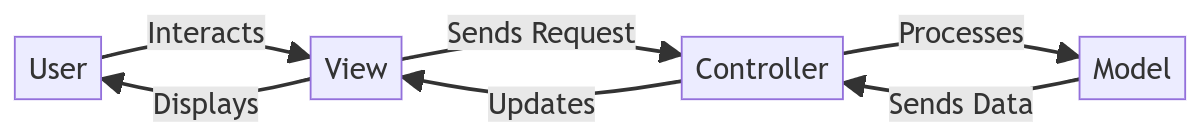
\includegraphics[width=\textwidth]{../figures/mvc-modern.png}
	\caption{Model View Controller Architecture}
	\label{fig:mvc_architecture}
\end{figure}

Pengguna berinteraksi dengan aplikasi melalui antarmuka pengguna yang dikenal sebagai View. View mencakup elemen-elemen seperti tombol, formulir, tabel, dan komponen visual lainnya yang memungkinkan pengguna memberikan input dan menerima output dari aplikasi. Sebagai contoh, dalam JavaFX, pengguna dapat mengklik tombol "Submit" pada sebuah formulir untuk memulai suatu aksi.

Ketika pengguna melakukan suatu aksi pada View, seperti mengklik tombol atau memasukkan teks, View akan mengirimkan permintaan tersebut ke Controller. View tidak menangani logika pemrosesan sendiri, melainkan menyerahkan tugas tersebut kepada Controller. Dalam JavaFX, View dapat memicu metode di Controller melalui event handler seperti \texttt{onAction} pada sebuah tombol.

Controller menerima permintaan dari View dan kemudian memprosesnya dengan berinteraksi dengan Model. Model adalah komponen yang bertanggung jawab atas logika bisnis dan operasi data, seperti mengakses database, melakukan perhitungan, atau memanipulasi data aplikasi. Sebagai contoh, Controller dapat memanggil metode di Model untuk mendapatkan daftar produk dari database.

Setelah Model selesai memproses permintaan, Model akan mengirimkan data kembali ke Controller. Data ini bisa berupa hasil query dari database, hasil perhitungan, atau data yang telah diproses sesuai logika bisnis. Dalam JavaFX, Model mungkin mengembalikan daftar objek yang kemudian dapat digunakan oleh Controller untuk memperbarui tampilan aplikasi.

Controller kemudian mengambil data dari Model dan memperbarui View sesuai dengan data tersebut. Pembaruan ini mungkin melibatkan pengisian tabel dengan data baru, memperbarui teks di label, atau menampilkan notifikasi kepada pengguna. Sebagai contoh, Controller di JavaFX dapat memperbarui elemen \texttt{TableView} dengan data terbaru yang diterima dari Model.

Terakhir, View akan menampilkan data yang telah diperbarui kepada pengguna. Pengguna kemudian dapat melihat hasil dari aksi yang mereka lakukan sebelumnya, seperti melihat tabel produk yang sudah terisi dengan data terbaru. Proses ini menciptakan siklus interaksi antara pengguna dan aplikasi, di mana setiap aksi pengguna dapat memicu pembaruan View melalui Controller dan Model.


\section{Prasyarat Java dan MySQL}
Sebelum memulai pengembangan aplikasi JavaFX, pastikan bahwa perangkat lunak berikut telah terinstal:

\begin{itemize}
	\item Java Development Kit (JDK) minimal versi 11 atau lebih baru.
	\item MySQL sebagai basis data untuk penyimpanan data aplikasi.
	\item Driver JDBC MySQL agar Java dapat berkomunikasi dengan database.
	\item Gradle sebagai build tool untuk mengelola dependensi dan otomasi proses pembangunan proyek.
\end{itemize}

\section{Mengunduh dan Menginstal Gradle serta Konfigurasi Proyek Java dengan Gradle}

Gradle adalah alat otomatisasi pembangunan proyek yang banyak digunakan dalam pengembangan perangkat lunak modern. Untuk menginstalnya, unduh versi terbaru dari situs resmi Gradle dan pastikan variabel lingkungan telah dikonfigurasi dengan benar agar dapat diakses melalui terminal. Untuk menginstal Gradle di sistem berbasis Linux, ikuti pentunjuk pada tautan berikut \url{https://gradle.org/install/}.


Langkah-langkah untuk menginisialisasi proyek Java dengan Gradle:

\begin{enumerate}
\item Pastikan Gradle telah terinstal dengan menjalankan perintah berikut:
\begin{lstlisting}[language=bash]
gradle -v
\end{lstlisting}

\item Buat direktori proyek baru dan masuk ke dalamnya:
\begin{lstlisting}[language=bash]
mkdir my-java-project
cd my-java-project
\end{lstlisting}

\item Jalankan perintah berikut untuk menginisialisasi proyek Java dengan Gradle:
\begin{lstlisting}[language=bash]
gradle init --type java-application
\end{lstlisting}
\end{enumerate}

Dengan perintah di atas, Gradle akan langsung menginisialisasi proyek Java sebagai aplikasi, tanpa perlu memilih opsi secara manual. Proyek Java dengan Gradle telah berhasil dikonfigurasi dan siap digunakan untuk pengembangan aplikasi berbasis Java.

\section{Struktur Direktori Proyek}
Setelah Gradle dikonfigurasi, target \texttt{folder} dan \texttt{files} yang akan dibuat dalam proyek ini adalah sebagai berikut.

\begin{lstlisting}[language=bash]
	my-javafx-project/
	|-- app/
	|   |-- build.gradle
	|   |-- src/
	|   |   |-- main/
	|   |   |   |-- java/
	|   |   |   |   |-- org/example/controllers/
	|   |   |   |   |   |-- ItemController.java
	|   |   |   |   |   |-- MainController.java
	|   |   |   |   |   |-- SalesOrderController.java
	|   |   |   |   |   |-- SelectFormController.java
	|   |   |   |   |-- org/example/helpers/
	|   |   |   |   |   |-- IForm.java
	|   |   |   |   |-- org/example/models/
	|   |   |   |   |   |-- Item.java
	|   |   |   |   |   |-- Order.java
	|   |   |   |   |   |-- OrderDetail.java
	|   |   |   |   |   |-- OrderDetailPK.java
	|   |   |   |-- resources/
	|   |   |   |   |-- hibernate.cfg.xml
	|   |   |   |   |-- Item.fxml
	|   |   |   |   |-- Main.fxml
	|   |   |   |   |-- SalesOrder.fxml
	|   |   |   |   |-- SelectForm.fxml
	|   |   |   |   |-- test.rptdesign
	|-- settings.gradle
	|-- gradle.properties
	|-- gradlew
	|-- gradlew.bat
\end{lstlisting}


Struktur proyek JavaFX ini terdiri dari beberapa direktori dan file utama yang dikelompokkan berdasarkan fungsinya. Berikut adalah target direktori dan file yang digunakan dalam proyek ini:

\begin{enumerate}
	\item \textbf{Root Direktori}:
	\begin{itemize}
		\item \texttt{settings.gradle} - File konfigurasi Gradle yang mengatur pengelolaan proyek multi-modul.
		\item \texttt{gradle.properties} - File properti Gradle yang menyimpan konfigurasi global proyek.
		\item \texttt{gradlew} dan \texttt{gradlew.bat} - Skrip untuk menjalankan Gradle Wrapper di sistem Unix dan Windows.
	\end{itemize}
	
	\item \textbf{Direktori Aplikasi (app/)}:
	\begin{itemize}
		\item \texttt{build.gradle} - File konfigurasi Gradle yang mengelola dependensi dan pengaturan proyek aplikasi.
		\item \texttt{src/} - Direktori utama yang berisi kode sumber proyek.
	\end{itemize}
	
	\item \textbf{Direktori Kode Sumber (src/main/)}:
	\begin{itemize}
		\item \texttt{java/org/example/controllers/} - Berisi kelas \textbf{Controller} yang menangani logika aplikasi, seperti \texttt{ItemController.java}, \texttt{MainController.java}, dan lainnya.
		\item \texttt{java/org/example/helpers/} - Berisi kelas bantuan yang mendukung operasi aplikasi, seperti \texttt{IForm.java}.
		\item \texttt{java/org/example/models/} - Berisi \textbf{Model} data yang merepresentasikan entitas bisnis, seperti \texttt{Item.java}, \texttt{Order.java}, dan \texttt{OrderDetail.java}.
	\end{itemize}
	
	\item \textbf{Direktori Resource (src/main/resources/)}:
	\begin{itemize}
		\item \texttt{hibernate.cfg.xml} - Konfigurasi Hibernate untuk menghubungkan aplikasi dengan database.
		\item Berkas \textbf{View} JavaFX dalam format \texttt{FXML}, seperti \texttt{Item.fxml}, \texttt{Main.fxml}, \texttt{SalesOrder.fxml}, dan \texttt{SelectForm.fxml}.
		\item \texttt{test.rptdesign} - Template laporan yang digunakan dalam aplikasi.
	\end{itemize}
\end{enumerate}


\section{Konfigurasi Gradle}

File \texttt{build.gradle} dalam proyek ini mengatur konfigurasi build menggunakan Gradle. Berikut adalah kode lengkap yang digunakan dalam file tersebut:

\begin{lstlisting}[style=JavaStyle]
	plugins {
		id 'application'
		id 'org.openjfx.javafxplugin' version '0.1.0'
	}
	
	repositories {
		mavenCentral()
	}
	
	dependencies {
		implementation 'mysql:mysql-connector-java:8.0.33'
		implementation 'org.hibernate:hibernate-core:6.2.12.Final'
		implementation 'jakarta.persistence:jakarta.persistence-api:3.1.0'
		implementation "org.openjfx:javafx-controls:20.0.1"
		implementation "org.openjfx:javafx-fxml:20.0.1"
		implementation 'com.innoventsolutions.birt.runtime:org.eclipse.birt.runtime_4.8.0-20180626:4.8.0'
		
		testImplementation libs.junit.jupiter
		testRuntimeOnly 'org.junit.platform:junit-platform-launcher'
		implementation libs.guava
	}
	
	java {
		toolchain {
			languageVersion = JavaLanguageVersion.of(21)
		}
	}
	
	application {
		mainClass = 'org.example.Main'
	}
	
	tasks.named('test') {
		useJUnitPlatform()
	}
	
	javafx {
		version = "21.0.1"
		modules = [ 'javafx.controls', 'javafx.fxml' ]
	}
\end{lstlisting}

Bagian \texttt{plugins} mendefinisikan plugin yang digunakan dalam proyek. Plugin \texttt{application} digunakan untuk aplikasi Java biasa, sedangkan \texttt{org.openjfx.javafxplugin} digunakan untuk mendukung JavaFX.

Bagian \texttt{repositories} menentukan lokasi tempat dependensi akan diunduh. Dalam konfigurasi ini, proyek menggunakan \texttt{mavenCentral()} sebagai repositori utama.

Bagian \texttt{dependencies} mendefinisikan pustaka eksternal yang digunakan dalam proyek. MySQL Connector digunakan untuk koneksi ke database MySQL. Hibernate Core digunakan untuk Object-Relational Mapping (ORM) dan manajemen database. Jakarta Persistence API merupakan API standar untuk ORM berbasis Java. JavaFX Controls dan JavaFX FXML menyediakan komponen antarmuka pengguna untuk JavaFX. BIRT Runtime digunakan untuk rendering laporan dalam aplikasi. JUnit dan Guava digunakan untuk pengujian unit dan utilitas tambahan dalam Java.

Bagian \texttt{java.toolchain} memastikan bahwa proyek menggunakan Java 21 sebagai versi bahasa pemrograman yang dikompilasi. Bagian \texttt{application} mendefinisikan kelas utama yang akan dijalankan dalam aplikasi, dalam hal ini \texttt{org.example.Main}. Bagian \texttt{tasks.named('test')} mengonfigurasi Gradle untuk menggunakan JUnit Platform sebagai framework pengujian. Bagian \texttt{javafx} menentukan versi JavaFX yang digunakan serta modul yang diperlukan dalam aplikasi.

\section{Konfigurasi Hibernate}

File \texttt{hibernate.cfg.xml} digunakan untuk mengonfigurasi Hibernate sebagai ORM (Object-Relational Mapping) yang menghubungkan aplikasi Java dengan database MySQL. Berikut adalah kode konfigurasi yang digunakan:

\begin{lstlisting}[style=XmlStyle]
	<?xml version="1.0" encoding="utf-8"?>
	<!DOCTYPE hibernate-configuration PUBLIC 
	"-//Hibernate/Hibernate Configuration DTD 3.0//EN"
	"http://www.hibernate.org/dtd/hibernate-configuration-3.0.dtd">
	<hibernate-configuration>
	<session-factory>
	<!-- Database Configuration -->
	<property name="hibernate.connection.driver_class">com.mysql.cj.jdbc.Driver</property>
	<property name="hibernate.connection.url">jdbc:mysql://localhost:3306/pradita?useSSL=false&amp;serverTimezone=UTC</property>
	<property name="hibernate.connection.username">alfa</property>
	<property name="hibernate.connection.password">1234</property>
	
	<!-- Hibernate Settings -->
	<property name="hibernate.dialect">org.hibernate.dialect.MySQLDialect</property>
	<property name="hibernate.show_sql">true</property>
	<property name="hibernate.format_sql">true</property>
	<property name="hibernate.hbm2ddl.auto">update</property>
	
	<!-- Entity Mappings -->
	<mapping class="org.example.models.Order"/>
	<mapping class="org.example.models.OrderDetail"/>
	<mapping class="org.example.models.Item"/>
	</session-factory>
	</hibernate-configuration>
\end{lstlisting}

Konfigurasi ini terdiri dari beberapa bagian utama yang mengatur koneksi database, konfigurasi Hibernate, dan pemetaan entitas.

Bagian pertama adalah pengaturan koneksi ke database MySQL, termasuk driver yang digunakan, URL koneksi, username, dan password. Database yang digunakan dalam konfigurasi ini adalah \texttt{pradita} yang berada di \texttt{localhost} dengan timezone UTC dan tanpa SSL. Parameter \texttt{hibernate.connection.driver\_class} menentukan driver JDBC untuk MySQL. \texttt{hibernate.connection.url} berisi alamat database, sedangkan \texttt{hibernate.connection.username} dan \texttt{hibernate.connection.password} digunakan untuk autentikasi koneksi.

Bagian berikutnya adalah pengaturan Hibernate yang mencakup beberapa properti utama. \texttt{hibernate.dialect} menentukan dialect SQL yang digunakan, dalam hal ini \texttt{MySQLDialect}, agar Hibernate dapat menghasilkan query yang sesuai dengan MySQL. \texttt{hibernate.show\_sql} diatur ke \texttt{true} agar semua query SQL yang dieksekusi dapat dilihat di log, sedangkan \texttt{hibernate.format\_sql} digunakan untuk menampilkan query dalam format yang lebih rapi. Opsi \texttt{hibernate.hbm2ddl.auto} diset ke \texttt{update}, yang memungkinkan Hibernate secara otomatis menyesuaikan struktur tabel database dengan entitas Java.

Bagian terakhir adalah pemetaan entitas yang menentukan kelas-kelas model dalam paket \texttt{org.example.models} yang akan dikelola oleh Hibernate. Konfigurasi ini mencakup tiga kelas utama, yaitu \texttt{Order}, \texttt{OrderDetail}, dan \texttt{Item}. Dengan pengaturan ini, Hibernate dapat menghubungkan kelas-kelas model dengan tabel dalam database secara otomatis dan melakukan operasi CRUD tanpa perlu menulis query SQL manual.

\section{Models}
Dalam arsitektur perangkat lunak berbasis Model-View-Controller (MVC), \textbf{Model} berperan sebagai representasi data dan logika bisnis yang berinteraksi langsung dengan database. Model bertanggung jawab untuk menyimpan, mengelola, dan memanipulasi data yang digunakan dalam aplikasi. Dengan menggunakan Hibernate sebagai ORM (Object-Relational Mapping), setiap entitas dalam model dipetakan ke dalam tabel database, memungkinkan operasi \textbf{CRUD (Create, Read, Update, Delete)} dilakukan secara efisien tanpa perlu menulis query SQL secara manual. Setiap model dalam aplikasi didefinisikan sebagai kelas Java dengan anotasi \texttt{jakarta.persistence} untuk mendeklarasikan hubungan antara atribut dalam kode dengan kolom dalam tabel database. Bagian ini akan membahas berbagai entitas dalam aplikasi, termasuk \texttt{Item}, \texttt{Order}, dan \texttt{OrderDetail}, serta bagaimana masing-masing kelas diimplementasikan dalam Hibernate.

\subsection{Item.java}

File \texttt{Item.java} merupakan kelas entitas yang dipetakan ke tabel \texttt{item} dalam database menggunakan Hibernate. Berikut adalah kode sumbernya:

\begin{lstlisting}[style=JavaStyle]
	package org.example.models;
	
	import jakarta.persistence.Column;
	import jakarta.persistence.Entity;
	import jakarta.persistence.Id;
	import jakarta.persistence.Table;
	
	@Entity
	@Table(name = "item")
	public class Item {
		@Id
		@Column(name = "code", length = 5, nullable = false)
		private String code;
		
		@Column(name = "name", length = 50)
		private String name;
		
		@Column(name = "price", nullable = false)
		private Double price;
		
		@Column(name = "quantity", nullable = false)
		private Double quantity;
		
		// Getters and setters
		public String getCode() { return code; }
		public void setCode(String code) { this.code = code; }
		
		public String getName() { return name; }
		public void setName(String name) { this.name = name; }
		
		public Double getPrice() { return price; }
		public void setPrice(Double price) { this.price = price; }
		
		public Double getQuantity() { return quantity; }
		public void setQuantity(Double quantity) { this.quantity = quantity; }
	}
\end{lstlisting}

Kelas \texttt{Item} menggunakan beberapa anotasi dari \texttt{jakarta.persistence} yang memungkinkan Hibernate untuk memetakan objek Java ke tabel database. \textbf{Setiap anotasi memiliki fungsi spesifik} dalam proses ORM (Object-Relational Mapping) yang dilakukan oleh Hibernate.

\begin{enumerate}
	\item \textbf{Anotasi \texttt{@Entity}}. 
	Anotasi \texttt{@Entity} menandakan bahwa kelas ini merupakan entitas yang akan dipetakan ke dalam tabel database. Hibernate akan mengelola objek dari kelas ini dan menyimpannya dalam database.
	
	\item \textbf{Anotasi \texttt{@Table(name = \"item\")}}. 
	Anotasi \texttt{@Table(name = "item")} mengaitkan kelas \texttt{Item} dengan tabel \texttt{item} dalam database. Jika anotasi ini tidak diberikan, secara default Hibernate akan menggunakan nama kelas sebagai nama tabel.
	
	\item \textbf{Anotasi \texttt{@Id}}. 
	Atribut \texttt{code} digunakan sebagai primary key dari tabel \texttt{item}. Anotasi \texttt{@Id} menandakan bahwa atribut ini adalah kolom unik yang digunakan oleh Hibernate untuk mengidentifikasi setiap entitas dalam database.
	
	\item \textbf{Anotasi \texttt{@Column}}.
	Anotasi \texttt{@Column} digunakan untuk mendefinisikan properti yang akan dipetakan ke dalam kolom tabel database:
	\begin{enumerate}
		\item \texttt{@Column(name = "code", length = 5, nullable = false)} - Kolom \texttt{code} memiliki panjang maksimum 5 karakter dan tidak boleh kosong (\texttt{nullable = false}). Properti ini berfungsi sebagai primary key.
		\item \texttt{@Column(name = "name", length = 50)} - Kolom \texttt{name} memiliki panjang maksimum 50 karakter. Tidak ada batasan \texttt{nullable}, sehingga dapat diisi atau dibiarkan kosong.
		\item \texttt{@Column(name = "price", nullable = false)} - Kolom \texttt{price} menggunakan tipe data \texttt{Double} dan wajib diisi (\texttt{nullable = false}).
		\item \texttt{@Column(name = "quantity", nullable = false)} - Kolom \texttt{quantity} juga menggunakan tipe data \texttt{Double} dan wajib diisi (\texttt{nullable = false}).
	\end{enumerate}
	
	\item \textbf{Penggunaan Getter dan Setter}.
	Setiap atribut memiliki metode getter dan setter. Hibernate membutuhkan metode ini untuk membaca dan memperbarui nilai dari setiap atribut saat melakukan operasi database.

\end{enumerate}

Dengan konfigurasi ini, Hibernate akan melakukan pemetaan tabel \texttt{item} sebagai berikut:
\begin{enumerate}
	\item Setiap objek \texttt{Item} akan diperlakukan sebagai satu baris data dalam tabel \texttt{item}.
	\item Jika sebuah objek \texttt{Item} disimpan menggunakan Hibernate, maka Hibernate akan mengeksekusi query \texttt{INSERT} ke dalam database.
	\item Jika sebuah objek \texttt{Item} diubah, Hibernate akan secara otomatis menjalankan query \texttt{UPDATE} untuk menyimpan perubahan tersebut.
	\item Jika sebuah objek \texttt{Item} dihapus, Hibernate akan menjalankan query \texttt{DELETE}.
\end{enumerate}

Sebagai contoh, ketika kita menyimpan objek baru menggunakan Hibernate:

\begin{lstlisting}[style=JavaStyle]
	Session session = HibernateUtil.getSessionFactory().openSession();
	Transaction transaction = session.beginTransaction();
	
	Item item = new Item();
	item.setCode("A123");
	item.setName("Laptop");
	item.setPrice(15000000.0);
	item.setQuantity(10.0);
	
	session.save(item);
	transaction.commit();
	session.close();
\end{lstlisting}

Kode di atas akan menyebabkan Hibernate mengeksekusi query berikut dalam database:

\begin{lstlisting}[style=sql]
	INSERT INTO item (code, name, price, quantity) 
	VALUES ('A123', 'Laptop', 15000000.0, 10.0);
\end{lstlisting}

Jika kita ingin mengambil data berdasarkan kode barang:

\begin{lstlisting}[style=JavaStyle]
	Session session = HibernateUtil.getSessionFactory().openSession();
	Item item = session.get(Item.class, "A123");
	System.out.println("Nama Barang: " + item.getName());
	session.close();
\end{lstlisting}

Hibernate akan menerjemahkannya ke dalam query SQL berikut:

\begin{lstlisting}[style=sql]
	SELECT * FROM item WHERE code = 'A123';
\end{lstlisting}

Dengan pemetaan ini, Hibernate dapat menangani interaksi dengan database secara otomatis tanpa perlu menulis query SQL secara manual. Hal ini membuat pengelolaan database lebih efisien dan mengurangi ketergantungan pada query SQL yang eksplisit.


\subsection{Order.java}

File \texttt{Order.java} merupakan kelas entitas yang dipetakan ke tabel \texttt{order} dalam database menggunakan Hibernate. Kelas ini berfungsi sebagai model yang merepresentasikan pesanan dalam aplikasi. Berikut adalah kode sumbernya:

\begin{lstlisting}[style=JavaStyle]
	package org.example.models;
	
	import java.time.LocalDateTime;
	import java.util.List;
	
	import jakarta.persistence.CascadeType;
	import jakarta.persistence.Column;
	import jakarta.persistence.Entity;
	import jakarta.persistence.Id;
	import jakarta.persistence.OneToMany;
	import jakarta.persistence.Table;
	
	@Entity
	@Table(name = "order")
	public class Order {
		@Id
		@Column(name = "code", length = 5, nullable = false)
		private String code;
		
		@Column(name = "note", columnDefinition = "TEXT")
		private String note;
		
		@Column(name = "date", columnDefinition = "DATETIME DEFAULT CURRENT_TIMESTAMP")
		private LocalDateTime date;
		
		@OneToMany(mappedBy = "order", cascade = CascadeType.ALL, orphanRemoval = true)
		private List<OrderDetail> orderDetails;
		
		// Getters and setters
		public String getCode() { return code; }
		public void setCode(String code) { this.code = code; }
		
		public String getNote() { return note; }
		public void setNote(String note) { this.note = note; }
		
		public LocalDateTime getDate() { return date; }
		public void setDate(LocalDateTime date) { this.date = date; }
		
		public List<OrderDetail> getOrderDetails() { return orderDetails; }
		public void setOrderDetails(List<OrderDetail> orderDetails) { this.orderDetails = orderDetails; }
	}
\end{lstlisting}

Kelas \texttt{Order} menggunakan beberapa anotasi dari \texttt{jakarta.persistence} yang memungkinkan Hibernate untuk memetakan objek Java ke tabel database.

\begin{enumerate}
	\item \textbf{Anotasi \texttt{@Entity}}. 
	Anotasi \texttt{@Entity} menandakan bahwa kelas ini merupakan entitas yang akan dipetakan ke dalam tabel database. Hibernate akan mengelola objek dari kelas ini dan menyimpannya dalam database.
	
	\item \textbf{Anotasi \texttt{@Table(name = "order")}}. 
	Anotasi \texttt{@Table(name = "order")} mengaitkan kelas \texttt{Order} dengan tabel \texttt{order} dalam database. Jika anotasi ini tidak diberikan, secara default Hibernate akan menggunakan nama kelas sebagai nama tabel.
	
	\item \textbf{Anotasi \texttt{@Id}}. 
	Atribut \texttt{code} digunakan sebagai primary key dari tabel \texttt{order}. Anotasi \texttt{@Id} menandakan bahwa atribut ini adalah kolom unik yang digunakan oleh Hibernate untuk mengidentifikasi setiap entitas dalam database.
	
	\item \textbf{Anotasi \texttt{@Column}}.
	Anotasi \texttt{@Column} digunakan untuk mendefinisikan properti yang akan dipetakan ke dalam kolom tabel database:
	\begin{enumerate}
		\item \texttt{@Column(name = "code", length = 5, nullable = false)} - Kolom \texttt{code} memiliki panjang maksimum 5 karakter dan tidak boleh kosong (\texttt{nullable = false}). Properti ini berfungsi sebagai primary key.
		\item \texttt{@Column(name = "note", columnDefinition = "TEXT")} - Kolom \texttt{note} digunakan untuk menyimpan catatan pesanan dalam format teks panjang.
		\item \texttt{@Column(name = "date", columnDefinition = "DATETIME DEFAULT CURRENT\_TIMESTAMP")} - Kolom \texttt{date} menyimpan waktu pembuatan pesanan dengan nilai default \texttt{CURRENT\_TIMESTAMP}.
	\end{enumerate}
	
	\item \textbf{Anotasi \texttt{@OneToMany}}.
	Atribut \texttt{orderDetails} direpresentasikan sebagai daftar (\texttt{List}) yang berisi \texttt{OrderDetail}. 
	\begin{enumerate}
		\item \texttt{@OneToMany(mappedBy = "order", cascade = CascadeType.ALL, orphanRemoval = true)} \\
		Anotasi ini menunjukkan bahwa hubungan antara \texttt{Order} dan \texttt{OrderDetail} adalah **one-to-many**.
		\begin{itemize}
			\item \texttt{mappedBy = "order"} - Menunjukkan bahwa hubungan ini dikendalikan oleh atribut \texttt{order} dalam kelas \texttt{OrderDetail}.
			\item \texttt{cascade = CascadeType.ALL} - Jika entitas \texttt{Order} dibuat, diperbarui, atau dihapus, maka semua \texttt{OrderDetail} yang terkait akan ikut diperbarui atau dihapus.
			\item \texttt{orphanRemoval = true} - Jika sebuah \texttt{OrderDetail} tidak lagi terkait dengan entitas \texttt{Order}, maka entitas tersebut akan dihapus dari database.
		\end{itemize}
	\end{enumerate}
	
	\item \textbf{Penggunaan Getter dan Setter}.
	Setiap atribut memiliki metode getter dan setter. Hibernate membutuhkan metode ini untuk membaca dan memperbarui nilai dari setiap atribut saat melakukan operasi database.
	
\end{enumerate}

Dengan konfigurasi ini, Hibernate akan melakukan pemetaan tabel \texttt{order} sebagai berikut:
\begin{enumerate}
	\item Setiap objek \texttt{Order} akan diperlakukan sebagai satu baris data dalam tabel \texttt{order}.
	\item Jika sebuah objek \texttt{Order} disimpan menggunakan Hibernate, maka Hibernate akan mengeksekusi query \texttt{INSERT} ke dalam database.
	\item Jika sebuah objek \texttt{Order} diubah, Hibernate akan secara otomatis menjalankan query \texttt{UPDATE} untuk menyimpan perubahan tersebut.
	\item Jika sebuah objek \texttt{Order} dihapus, Hibernate akan menjalankan query \texttt{DELETE}.
\end{enumerate}

Sebagai contoh, ketika kita menyimpan objek baru menggunakan Hibernate:

\begin{lstlisting}[style=JavaStyle]
	Session session = HibernateUtil.getSessionFactory().openSession();
	Transaction transaction = session.beginTransaction();
	
	Order order = new Order();
	order.setCode("O123");
	order.setNote("Pesanan pertama");
	order.setDate(LocalDateTime.now());
	
	session.save(order);
	transaction.commit();
	session.close();
\end{lstlisting}

Kode di atas akan menyebabkan Hibernate mengeksekusi query berikut dalam database:

\begin{lstlisting}[style=sql]
	INSERT INTO `order` (code, note, date) 
	VALUES ('O123', 'Pesanan pertama', CURRENT_TIMESTAMP);
\end{lstlisting}

Jika kita ingin mengambil data berdasarkan kode pesanan:

\begin{lstlisting}[style=JavaStyle]
	Session session = HibernateUtil.getSessionFactory().openSession();
	Order order = session.get(Order.class, "O123");
	System.out.println("Catatan Pesanan: " + order.getNote());
	session.close();
\end{lstlisting}

Hibernate akan menerjemahkannya ke dalam query SQL berikut:

\begin{lstlisting}[style=sql]
	SELECT * FROM `order` WHERE code = 'O123';
\end{lstlisting}

Dengan pemetaan ini, Hibernate dapat menangani interaksi dengan database secara otomatis tanpa perlu menulis query SQL secara manual. Konfigurasi ini memastikan bahwa hubungan antara pesanan dan detail pesanan dapat dikelola dengan baik oleh Hibernate.


\subsection{OrderDetail.java}

File \texttt{OrderDetail.java} merupakan kelas entitas yang dipetakan ke tabel \texttt{order\_detail} dalam database menggunakan Hibernate. Kelas ini menyimpan detail pesanan yang terkait dengan pesanan utama dalam aplikasi. Berikut adalah kode sumbernya:

\begin{lstlisting}[style=JavaStyle]
	package org.example.models;
	
	import jakarta.persistence.Column;
	import jakarta.persistence.EmbeddedId;
	import jakarta.persistence.Entity;
	import jakarta.persistence.JoinColumn;
	import jakarta.persistence.ManyToOne;
	import jakarta.persistence.MapsId;
	import jakarta.persistence.Table;
	
	@Entity
	@Table(name = "order_detail")
	public class OrderDetail {
		@EmbeddedId
		private OrderDetailPK id;
		
		@ManyToOne
		@MapsId("orderCode")
		@JoinColumn(name = "code", nullable = false)
		private Order order;
		
		@Column(name = "itemcode", length = 5, nullable = false)
		private String itemCode;
		
		@Column(name = "name", length = 50)
		private String name;
		
		@Column(name = "price", nullable = false)
		private Double price;
		
		@Column(name = "quantity", nullable = false)
		private Double quantity;
		
		public OrderDetail(OrderDetailPK id, Order order, String itemCode, String name, double price, double quantity) {
			this.id = id;
			this.order = order;
			this.itemCode = itemCode;
			this.name = name;
			this.price = price;
			this.quantity = quantity;
		}
		
		// Getters and setters
		public OrderDetailPK getId() { return id; }
		public void setId(OrderDetailPK id) { this.id = id; }
		
		public Order getOrder() { return order; }
		public void setOrder(Order order) { this.order = order; }
		
		public String getItemCode() { return itemCode; }
		public void setItemCode(String itemCode) { this.itemCode = itemCode; }
		
		public String getName() { return name; }
		public void setName(String name) { this.name = name; }
		
		public Double getPrice() { return price; }
		public void setPrice(Double price) { this.price = price; }
		
		public Double getQuantity() { return quantity; }
		public void setQuantity(Double quantity) { this.quantity = quantity; }
	}
\end{lstlisting}

Kelas \texttt{OrderDetail} menggunakan beberapa anotasi dari \texttt{jakarta.persistence} yang memungkinkan Hibernate untuk memetakan objek Java ke tabel database.

\begin{enumerate}
	\item \textbf{Anotasi \texttt{@Entity}}. 
	Anotasi \texttt{@Entity} menandakan bahwa kelas ini merupakan entitas yang akan dipetakan ke dalam tabel database. Hibernate akan mengelola objek dari kelas ini dan menyimpannya dalam database.
	
	\item \textbf{Anotasi \texttt{@Table(name = "order\_detail")}}. 
	Anotasi \texttt{@Table(name = "order\_detail")} mengaitkan kelas \texttt{OrderDetail} dengan tabel \texttt{order\_detail} dalam database.
	
	\item \textbf{Anotasi \texttt{@EmbeddedId}}. 
	Anotasi \texttt{@EmbeddedId} menunjukkan bahwa primary key dari entitas ini terdiri dari beberapa kolom yang dikelola dalam kelas \texttt{OrderDetailPK}.
	
	\item \textbf{Anotasi \texttt{@ManyToOne}}. 
	Anotasi \texttt{@ManyToOne} menunjukkan bahwa entitas ini memiliki relasi **many-to-one** dengan \texttt{Order}, di mana banyak \texttt{OrderDetail} dapat terkait dengan satu \texttt{Order}.
	
	\item \textbf{Anotasi \texttt{@MapsId}}. 
	Anotasi \texttt{@MapsId("orderCode")} menunjukkan bahwa nilai primary key dari \texttt{OrderDetail} akan menggunakan primary key dari \texttt{Order}.
	
	\item \textbf{Anotasi \texttt{@JoinColumn}}. 
	Anotasi \texttt{@JoinColumn(name = "code", nullable = false)} menentukan bahwa kolom \texttt{code} adalah foreign key yang menghubungkan entitas ini dengan tabel \texttt{order}.
	
	\item \textbf{Anotasi \texttt{@Column}}. 
	Anotasi \texttt{@Column} digunakan untuk mendefinisikan properti yang akan dipetakan ke dalam kolom tabel database:
	\begin{enumerate}
		\item \texttt{@Column(name = "itemcode", length = 5, nullable = false)} - Kolom \texttt{itemcode} menyimpan kode item dengan panjang maksimum 5 karakter dan tidak boleh kosong.
		\item \texttt{@Column(name = "name", length = 50)} - Kolom \texttt{name} menyimpan nama item dengan panjang maksimum 50 karakter.
		\item \texttt{@Column(name = "price", nullable = false)} - Kolom \texttt{price} menyimpan harga item dan wajib diisi.
		\item \texttt{@Column(name = "quantity", nullable = false)} - Kolom \texttt{quantity} menyimpan jumlah item dan wajib diisi.
	\end{enumerate}
	
	\item \textbf{Penggunaan Getter dan Setter}. 
	Setiap atribut memiliki metode getter dan setter. Hibernate membutuhkan metode ini untuk membaca dan memperbarui nilai dari setiap atribut saat melakukan operasi database.
\end{enumerate}

Dengan konfigurasi ini, Hibernate akan melakukan pemetaan tabel \texttt{order\_detail} sebagai berikut:
\begin{enumerate}
	\item Setiap objek \texttt{OrderDetail} akan diperlakukan sebagai satu baris data dalam tabel \texttt{order\_detail}.
	\item Jika sebuah objek \texttt{OrderDetail} disimpan menggunakan Hibernate, maka Hibernate akan mengeksekusi query \texttt{INSERT} ke dalam database.
	\item Jika sebuah objek \texttt{OrderDetail} diubah, Hibernate akan secara otomatis menjalankan query \texttt{UPDATE} untuk menyimpan perubahan tersebut.
	\item Jika sebuah objek \texttt{OrderDetail} dihapus, Hibernate akan menjalankan query \texttt{DELETE}.
\end{enumerate}

Sebagai contoh, ketika kita menyimpan objek baru menggunakan Hibernate:

\begin{lstlisting}[style=JavaStyle]
	Session session = HibernateUtil.getSessionFactory().openSession();
	Transaction transaction = session.beginTransaction();
	
	OrderDetailPK id = new OrderDetailPK("O123", "I567");
	Order order = session.get(Order.class, "O123");
	OrderDetail orderDetail = new OrderDetail(id, order, "I567", "Mouse", 50000.0, 2.0);
	
	session.save(orderDetail);
	transaction.commit();
	session.close();
\end{lstlisting}

Kode di atas akan menyebabkan Hibernate mengeksekusi query berikut dalam database:

\begin{lstlisting}[style=sql]
	INSERT INTO order_detail (code, itemcode, name, price, quantity) 
	VALUES ('O123', 'I567', 'Mouse', 50000.0, 2.0);
\end{lstlisting}

Dengan pemetaan ini, Hibernate dapat menangani interaksi dengan database secara otomatis tanpa perlu menulis query SQL secara manual. Konfigurasi ini memastikan bahwa hubungan antara detail pesanan dan pesanan utama dapat dikelola dengan baik oleh Hibernate.


\subsection{OrderDetailPK.java}

File \texttt{OrderDetailPK.java} merupakan kelas yang digunakan sebagai \textbf{primary key} komposit dalam entitas \texttt{OrderDetail}. Kelas ini berfungsi sebagai identifier unik yang terdiri dari beberapa kolom dalam tabel \texttt{order\_detail}. Berikut adalah kode sumbernya:

\begin{lstlisting}[style=JavaStyle]
	package org.example.models;
	
	import java.util.Objects;
	import jakarta.persistence.Column;
	import jakarta.persistence.Embeddable;
	
	@Embeddable
	public class OrderDetailPK implements java.io.Serializable {
		@Column(name = "code", length = 5, nullable = false)
		private String orderCode;
		
		@Column(name = "line", nullable = false)
		private Integer line;
		
		public OrderDetailPK(String newCode, int line) {
			this.orderCode = newCode;
			this.line = line;
		}
		
		// Getters, setters, equals, and hashCode
		public String getOrderCode() { return orderCode; }
		public void setOrderCode(String orderCode) { this.orderCode = orderCode; }
		
		public Integer getLine() { return line; }
		public void setLine(Integer line) { this.line = line; }
		
		@Override
		public boolean equals(Object o) {
			if (this == o)
			return true;
			if (o == null || getClass() != o.getClass())
			return false;
			OrderDetailPK that = (OrderDetailPK) o;
			return orderCode.equals(that.orderCode) && line.equals(that.line);
		}
		
		@Override
		public int hashCode() {
			return Objects.hash(orderCode, line);
		}
	}
\end{lstlisting}

Kelas \texttt{OrderDetailPK} menggunakan beberapa anotasi dari \texttt{jakarta.persistence} yang memungkinkan Hibernate untuk menangani primary key komposit.

\begin{enumerate}
	\item \textbf{Anotasi \texttt{@Embeddable}}. 
	Anotasi \texttt{@Embeddable} menandakan bahwa kelas ini digunakan untuk menjadi bagian dari primary key dalam kelas entitas lain, dalam hal ini \texttt{OrderDetail}.
	
	\item \textbf{Anotasi \texttt{@Column}}. 
	Anotasi \texttt{@Column} digunakan untuk mendefinisikan properti yang akan dipetakan ke dalam kolom tabel database:
	\begin{enumerate}
		\item \texttt{@Column(name = "code", length = 5, nullable = false)} - Kolom \texttt{code} berisi kode pesanan sebagai bagian dari primary key.
		\item \texttt{@Column(name = "line", nullable = false)} - Kolom \texttt{line} berfungsi sebagai nomor baris dalam pesanan.
	\end{enumerate}
	
	\item \textbf{Implementasi Interface \texttt{Serializable}}. 
	Kelas ini mengimplementasikan \texttt{java.io.Serializable} agar dapat digunakan sebagai primary key dalam Hibernate. Hibernate membutuhkan primary key komposit untuk dapat diubah menjadi representasi byte-stream.
	
	\item \textbf{Implementasi Metode \texttt{equals} dan \texttt{hashCode}}. 
	\begin{enumerate}
		\item Metode \texttt{equals()} digunakan untuk membandingkan dua objek \texttt{OrderDetailPK} berdasarkan \texttt{orderCode} dan \texttt{line}.
		\item Metode \texttt{hashCode()} digunakan untuk menghasilkan nilai hash berdasarkan atribut \texttt{orderCode} dan \texttt{line}, yang berguna untuk memastikan integritas data dalam koleksi seperti \texttt{HashSet} atau \texttt{HashMap}.
	\end{enumerate}
\end{enumerate}

Dengan konfigurasi ini, Hibernate akan melakukan pemetaan tabel \texttt{order\_detail} sebagai berikut:
\begin{enumerate}
	\item Setiap objek \texttt{OrderDetailPK} akan digunakan sebagai kunci unik dalam tabel \texttt{order\_detail}.
	\item Jika sebuah objek \texttt{OrderDetail} disimpan menggunakan Hibernate, maka kunci yang digunakan adalah gabungan dari \texttt{code} dan \texttt{line}.
	\item Jika sebuah objek \texttt{OrderDetail} dihapus, Hibernate akan mencari data berdasarkan primary key komposit ini sebelum menjalankan query \texttt{DELETE}.
\end{enumerate}

Sebagai contoh, ketika kita menyimpan objek baru menggunakan Hibernate:

\begin{lstlisting}[style=JavaStyle]
	Session session = HibernateUtil.getSessionFactory().openSession();
	Transaction transaction = session.beginTransaction();
	
	OrderDetailPK id = new OrderDetailPK("O123", 1);
	Order order = session.get(Order.class, "O123");
	OrderDetail orderDetail = new OrderDetail(id, order, "I567", "Mouse", 50000.0, 2.0);
	
	session.save(orderDetail);
	transaction.commit();
	session.close();
\end{lstlisting}

Kode di atas akan menyebabkan Hibernate mengeksekusi query berikut dalam database:

\begin{lstlisting}[style=sql]
	INSERT INTO order_detail (code, line, itemcode, name, price, quantity) 
	VALUES ('O123', 1, 'I567', 'Mouse', 50000.0, 2.0);
\end{lstlisting}

Dengan pemetaan ini, Hibernate dapat menangani interaksi dengan database secara otomatis tanpa perlu menulis query SQL secara manual. Konfigurasi ini memastikan bahwa setiap detail pesanan memiliki primary key unik yang terdiri dari kode pesanan dan nomor baris.

\section{Controllers}

\subsection{MainController.java}

Dalam aplikasi berbasis JavaFX, kelas \texttt{MainController} bertindak sebagai pengendali utama yang mengelola interaksi pengguna dengan antarmuka grafis dan menangani berbagai operasi bisnis. Kelas ini bertanggung jawab untuk membuka berbagai formulir, menangani koneksi ke database MySQL, serta menangani pembuatan dan pencetakan laporan menggunakan BIRT (Business Intelligence and Reporting Tools). Dengan memanfaatkan mekanisme \textbf{FXML}, JavaFX dapat memisahkan tampilan dan logika bisnis, sehingga pengelolaan antarmuka menjadi lebih modular dan mudah dikembangkan.

Berikut adalah kode sumber dari kelas \texttt{MainController}:

\begin{lstlisting}[style=JavaStyle]
package org.example.controllers;

import java.awt.Desktop;
import java.io.File;
import java.io.IOException;
import java.sql.Connection;
import java.sql.DriverManager;

import org.eclipse.birt.core.framework.Platform;
import org.eclipse.birt.report.engine.api.EngineConfig;
import org.eclipse.birt.report.engine.api.IReportEngine;
import org.eclipse.birt.report.engine.api.IReportEngineFactory;
import org.eclipse.birt.report.engine.api.IReportRunnable;
import org.eclipse.birt.report.engine.api.IRunAndRenderTask;
import org.eclipse.birt.report.engine.api.PDFRenderOption;
import org.example.helpers.IForm;

import javafx.fxml.FXML;
import javafx.fxml.FXMLLoader;
import javafx.scene.Parent;
import javafx.scene.control.Alert;
import javafx.scene.control.MenuItem;
import javafx.scene.layout.BorderPane;

public class MainController {

@FXML
private MenuItem menuItemPrint;
@FXML
private MenuItem menuItemClose;
@FXML
private MenuItem menuItemOpenItem;
@FXML
private MenuItem menuItemAbout;
@FXML
private MenuItem menuItemOpenSalesOrder;
@FXML
private BorderPane centerPane;
public static Connection CONNECTION;

private IForm currentForm;

public void initialize() {
try {
Class.forName("com.mysql.cj.jdbc.Driver");
CONNECTION = DriverManager.getConnection("jdbc:mysql://localhost:3306/pradita", "alfa", "1234");
} catch (Exception e) {
e.printStackTrace();
}
}

@FXML
private void openItem() {
try {
FXMLLoader loader = new FXMLLoader(getClass().getResource("/Item.fxml"));
Parent itemFormRoot = loader.load();
centerPane.setCenter(itemFormRoot);
currentForm = loader.getController();
} catch (IOException e) {
e.printStackTrace();
showAlert("Error", "Could not open Item Form.");
}
}

@FXML
private void openSalesOrder() {
try {
FXMLLoader loader = new FXMLLoader(getClass().getResource("/SalesOrder.fxml"));
Parent salesOrderRoot = loader.load();
centerPane.setCenter(salesOrderRoot);
currentForm = loader.getController();
} catch (IOException e) {
e.printStackTrace();
showAlert("Error", "Could not open Sales Order Form.");
}
}

@FXML
private void showAbout() {
Alert alert = new Alert(Alert.AlertType.INFORMATION);
alert.setTitle("About");
alert.setHeaderText("Order Form Application");
alert.setContentText("Developed with JavaFX and BIRT for report generation.");
alert.showAndWait();
}

@FXML
private void printReport() {
new Thread(() -> {
try {
EngineConfig config = new EngineConfig();
Platform.startup(config);
IReportEngineFactory factory = (IReportEngineFactory) Platform
.createFactoryObject(IReportEngineFactory.EXTENSION_REPORT_ENGINE_FACTORY);
IReportEngine engine = factory.createReportEngine(config);

IReportRunnable design = engine.openReportDesign("/data2/projects/pemrograman-berorientasi-objek/code/pertemuan_05/javafx/app/build/resources/main/test.rptdesign");
IRunAndRenderTask task = engine.createRunAndRenderTask(design);
task.setParameterValue("order_code", currentForm.getDocumentCode());
PDFRenderOption options = new PDFRenderOption();
options.setOutputFileName("document.pdf");
options.setOutputFormat("pdf");

task.setRenderOption(options);
task.run();
task.close();
engine.destroy();

if (Desktop.isDesktopSupported()) {
File myFile = new File("document.pdf");
Desktop.getDesktop().open(myFile);
}

} catch (Exception e) {
e.printStackTrace();
} finally {
Platform.shutdown();
}
}).start();
}

private void showAlert(String title, String message) {
Alert alert = new Alert(Alert.AlertType.ERROR);
alert.setTitle(title);
alert.setHeaderText(null);
alert.setContentText(message);
alert.showAndWait();
}
}
\end{lstlisting}

Kelas \texttt{MainController} memiliki beberapa fungsi utama:

\begin{enumerate}
\item \textbf{Inisialisasi Koneksi Database}.
Metode \texttt{initialize()} dipanggil saat aplikasi dijalankan untuk memulai koneksi ke database MySQL. Driver database dimuat menggunakan \texttt{Class.forName()}, lalu koneksi dibuat dengan \texttt{DriverManager.getConnection()}. Jika terjadi kesalahan, pengecualian ditangani dengan mencetak \texttt{stack trace}.

\item \textbf{Membuka Formulir Item dan Sales Order}.
Aplikasi ini memungkinkan pengguna untuk membuka formulir yang berbeda dengan menggunakan metode \texttt{openItem()} dan \texttt{openSalesOrder()}. Kedua metode ini menggunakan \texttt{FXMLLoader} untuk memuat file \texttt{.fxml} yang berisi tampilan dan menampilkannya dalam \texttt{centerPane}. Referensi controller dari tampilan yang dibuka disimpan dalam variabel \texttt{currentForm}.

\item \textbf{Menampilkan Dialog Informasi}.
Metode \texttt{showAbout()} menampilkan informasi tentang aplikasi menggunakan objek \texttt{Alert} dari JavaFX. Dialog ini menampilkan nama aplikasi dan informasi teknologi yang digunakan.

\item \textbf{Pencetakan Laporan dengan BIRT}.
Metode \texttt{printReport()} digunakan untuk menghasilkan laporan dalam format PDF. Laporan dibuka menggunakan BIRT dengan \texttt{IReportEngine}, kemudian parameter laporan ditetapkan menggunakan \texttt{setParameterValue()}. Laporan dijalankan dan diekspor dalam format PDF dengan \texttt{PDFRenderOption}. Setelah selesai, jika sistem mendukung fitur desktop, file PDF akan dibuka secara otomatis.

\item \textbf{Penanganan Kesalahan}.
Jika terjadi kesalahan dalam proses pemuatan tampilan atau pembuatan laporan, metode \texttt{showAlert()} digunakan untuk menampilkan pesan kesalahan kepada pengguna. Dialog kesalahan dibuat menggunakan objek \texttt{Alert} dari JavaFX.
\end{enumerate}

Dengan konfigurasi ini, \texttt{MainController} bertindak sebagai penghubung antara antarmuka pengguna dan logika bisnis dalam aplikasi. Kombinasi JavaFX dan BIRT memungkinkan aplikasi untuk menangani data dan menghasilkan laporan secara efektif. Dalam pengembangan lebih lanjut, pengelolaan koneksi database sebaiknya dilakukan melalui lapisan layanan (\textit{service layer}) untuk meningkatkan modularitas dan keamanan sistem.
\subsection{MainController.java}

Dalam aplikasi berbasis JavaFX, kelas \texttt{MainController} bertindak sebagai pengendali utama yang mengelola interaksi pengguna dengan antarmuka grafis dan menangani berbagai operasi bisnis. Kelas ini bertanggung jawab untuk membuka berbagai formulir, menangani koneksi ke database MySQL, serta menangani pembuatan dan pencetakan laporan menggunakan BIRT (Business Intelligence and Reporting Tools). Dengan memanfaatkan mekanisme \textbf{FXML}, JavaFX dapat memisahkan tampilan dan logika bisnis, sehingga pengelolaan antarmuka menjadi lebih modular dan mudah dikembangkan.

Berikut adalah kode sumber dari kelas \texttt{MainController}:

\begin{lstlisting}[style=JavaStyle]
	package org.example.controllers;
	
	import java.awt.Desktop;
	import java.io.File;
	import java.io.IOException;
	import java.sql.Connection;
	import java.sql.DriverManager;
	
	import org.eclipse.birt.core.framework.Platform;
	import org.eclipse.birt.report.engine.api.EngineConfig;
	import org.eclipse.birt.report.engine.api.IReportEngine;
	import org.eclipse.birt.report.engine.api.IReportEngineFactory;
	import org.eclipse.birt.report.engine.api.IReportRunnable;
	import org.eclipse.birt.report.engine.api.IRunAndRenderTask;
	import org.eclipse.birt.report.engine.api.PDFRenderOption;
	import org.example.helpers.IForm;
	
	import javafx.fxml.FXML;
	import javafx.fxml.FXMLLoader;
	import javafx.scene.Parent;
	import javafx.scene.control.Alert;
	import javafx.scene.control.MenuItem;
	import javafx.scene.layout.BorderPane;
	
	public class MainController {
		
		@FXML
		private MenuItem menuItemPrint;
		@FXML
		private MenuItem menuItemClose;
		@FXML
		private MenuItem menuItemOpenItem;
		@FXML
		private MenuItem menuItemAbout;
		@FXML
		private MenuItem menuItemOpenSalesOrder;
		@FXML
		private BorderPane centerPane;
		public static Connection CONNECTION;
		
		private IForm currentForm;
		
		public void initialize() {
			System.out.println("Main Controller Initialized");
		}
		
		@FXML
		private void openItem() {
			try {
				FXMLLoader loader = new FXMLLoader(getClass().getResource("/Item.fxml"));
				Parent itemFormRoot = loader.load();
				centerPane.setCenter(itemFormRoot);
				currentForm = loader.getController();
			} catch (IOException e) {
				e.printStackTrace();
				showAlert("Error", "Could not open Item Form.");
			}
		}
		
		@FXML
		private void openSalesOrder() {
			try {
				FXMLLoader loader = new FXMLLoader(getClass().getResource("/SalesOrder.fxml"));
				Parent salesOrderRoot = loader.load();
				centerPane.setCenter(salesOrderRoot);
				currentForm = loader.getController();
			} catch (IOException e) {
				e.printStackTrace();
				showAlert("Error", "Could not open Sales Order Form.");
			}
		}
		
		@FXML
		private void showAbout() {
			Alert alert = new Alert(Alert.AlertType.INFORMATION);
			alert.setTitle("About");
			alert.setHeaderText("Order Form Application");
			alert.setContentText("Developed with JavaFX and BIRT for report generation.");
			alert.showAndWait();
		}
		
		@FXML
		private void printReport() {
			new Thread(() -> {
				try {
					EngineConfig config = new EngineConfig();
					Platform.startup(config);
					IReportEngineFactory factory = (IReportEngineFactory) Platform
					.createFactoryObject(IReportEngineFactory.EXTENSION_REPORT_ENGINE_FACTORY);
					IReportEngine engine = factory.createReportEngine(config);
					
					IReportRunnable design = engine.openReportDesign("/data2/projects/pemrograman-berorientasi-objek/code/pertemuan_05/javafx/app/build/resources/main/test.rptdesign");
					IRunAndRenderTask task = engine.createRunAndRenderTask(design);
					task.setParameterValue("order_code", currentForm.getDocumentCode());
					PDFRenderOption options = new PDFRenderOption();
					options.setOutputFileName("document.pdf");
					options.setOutputFormat("pdf");
					
					task.setRenderOption(options);
					task.run();
					task.close();
					engine.destroy();
					
					if (Desktop.isDesktopSupported()) {
						File myFile = new File("document.pdf");
						Desktop.getDesktop().open(myFile);
					}
					
				} catch (Exception e) {
					e.printStackTrace();
				} finally {
					Platform.shutdown();
				}
			}).start();
		}
		
		private void showAlert(String title, String message) {
			Alert alert = new Alert(Alert.AlertType.ERROR);
			alert.setTitle(title);
			alert.setHeaderText(null);
			alert.setContentText(message);
			alert.showAndWait();
		}
	}
\end{lstlisting}

Kelas \texttt{MainController} memiliki beberapa fungsi utama:

\begin{enumerate}
	\item \textbf{Inisialisasi Koneksi Database}.  
	Metode \texttt{initialize()} dipanggil saat aplikasi dijalankan untuk memulai koneksi ke database MySQL. Driver database dimuat menggunakan \texttt{Class.forName()}, lalu koneksi dibuat dengan \texttt{DriverManager.getConnection()}. Jika terjadi kesalahan, pengecualian ditangani dengan mencetak \texttt{stack trace}.
	
	\item \textbf{Membuka Formulir Item dan Sales Order}.  
	Aplikasi ini memungkinkan pengguna untuk membuka formulir yang berbeda dengan menggunakan metode \texttt{openItem()} dan \texttt{openSalesOrder()}. Kedua metode ini menggunakan \texttt{FXMLLoader} untuk memuat file \texttt{.fxml} yang berisi tampilan dan menampilkannya dalam \texttt{centerPane}. Referensi controller dari tampilan yang dibuka disimpan dalam variabel \texttt{currentForm}.
	
	\item \textbf{Menampilkan Dialog Informasi}.  
	Metode \texttt{showAbout()} menampilkan informasi tentang aplikasi menggunakan objek \texttt{Alert} dari JavaFX. Dialog ini menampilkan nama aplikasi dan informasi teknologi yang digunakan.
	
	\item \textbf{Pencetakan Laporan dengan BIRT}.  
	Metode \texttt{printReport()} digunakan untuk menghasilkan laporan dalam format PDF. Laporan dibuka menggunakan BIRT dengan \texttt{IReportEngine}, kemudian parameter laporan ditetapkan menggunakan \texttt{setParameterValue()}. Laporan dijalankan dan diekspor dalam format PDF dengan \texttt{PDFRenderOption}. Setelah selesai, jika sistem mendukung fitur desktop, file PDF akan dibuka secara otomatis.
	
	\item \textbf{Penanganan Kesalahan}.  
	Jika terjadi kesalahan dalam proses pemuatan tampilan atau pembuatan laporan, metode \texttt{showAlert()} digunakan untuk menampilkan pesan kesalahan kepada pengguna. Dialog kesalahan dibuat menggunakan objek \texttt{Alert} dari JavaFX.
\end{enumerate}

Dengan konfigurasi ini, \texttt{MainController} bertindak sebagai penghubung antara antarmuka pengguna dan logika bisnis dalam aplikasi. Kombinasi JavaFX dan BIRT memungkinkan aplikasi untuk menangani data dan menghasilkan laporan secara efektif. Dalam pengembangan lebih lanjut, pengelolaan koneksi database sebaiknya dilakukan melalui lapisan layanan (\textit{service layer}) untuk meningkatkan modularitas dan keamanan sistem.



	\chapter{Unified Modeling Language (UML): Structural Diagram}

\section{Pendahuluan}
UML (Unified Modeling Language) adalah bahasa pemodelan yang digunakan untuk mendeskripsikan, merancang, dan mendokumentasikan sistem perangkat lunak. UML menyediakan berbagai jenis diagram yang dikategorikan menjadi diagram struktural dan diagram perilaku. Pada chapter ini, akan dibahas diagram struktural dalam UML.

Diagram struktural digunakan untuk menggambarkan bagian-bagian statis dari suatu sistem perangkat lunak. Diagram ini menunjukkan bagaimana kelas, objek, dan komponen lainnya disusun dalam sistem.


\section{Unified Modeling Language (UML) dan Sejarahnya}

Unified Modeling Language (UML) adalah standar pemodelan visual yang digunakan dalam rekayasa perangkat lunak untuk mendeskripsikan, merancang, dan mendokumentasikan sistem perangkat lunak. UML menyediakan sekumpulan diagram yang membantu pengembang dalam memahami struktur dan perilaku sistem sebelum implementasi.

\subsection{Sejarah UML}

UML dikembangkan pada pertengahan tahun 1990-an sebagai hasil dari penggabungan berbagai metode pemodelan perangkat lunak yang telah ada sebelumnya. Sebelum UML, terdapat beberapa metode pemodelan yang digunakan secara luas, seperti:
\begin{itemize}
	\item \textbf{Booch Method} – Dikembangkan oleh Grady Booch, metode ini digunakan untuk analisis dan desain sistem berbasis objek.
	\item \textbf{Object Modeling Technique (OMT)} – Dikembangkan oleh James Rumbaugh, metode ini berfokus pada pemodelan sistem berbasis objek dengan berbagai perspektif.
	\item \textbf{Object-Oriented Software Engineering (OOSE)} – Dikembangkan oleh Ivar Jacobson, metode ini memperkenalkan konsep \textit{use case} dalam pengembangan perangkat lunak.
\end{itemize}

Pada tahun 1994, Grady Booch, James Rumbaugh, dan Ivar Jacobson mulai bekerja sama untuk mengembangkan standar pemodelan terpadu. Mereka dikenal sebagai \textbf{Three Amigos} dalam dunia rekayasa perangkat lunak. Upaya mereka menghasilkan versi awal UML yang kemudian diserahkan kepada Object Management Group (OMG) pada tahun 1997 untuk standarisasi.

\subsection{Perkembangan UML}
Setelah disetujui oleh OMG, UML terus berkembang dengan berbagai revisi dan penyempurnaan. Beberapa tonggak penting dalam perkembangan UML meliputi:
\begin{itemize}
	\item \textbf{UML 1.0 (1997)} – Versi pertama yang distandarisasi oleh OMG.
	\item \textbf{UML 1.3 (1999)} – Peningkatan dalam elemen diagram dan dukungan lebih baik untuk pengembangan perangkat lunak berbasis objek.
	\item \textbf{UML 2.0 (2005)} – Pembaruan besar yang mencakup lebih banyak jenis diagram, seperti \textit{interaction overview diagram} dan peningkatan dalam ekspresi perilaku sistem.
	\item \textbf{UML versi terbaru} – UML terus diperbarui oleh OMG untuk mendukung perkembangan teknologi perangkat lunak.
\end{itemize}

\subsection{Penerapan UML dalam Rekayasa Perangkat Lunak}
Saat ini, UML digunakan secara luas dalam berbagai bidang rekayasa perangkat lunak, termasuk:
\begin{itemize}
	\item Pengembangan sistem berbasis objek.
	\item Pemodelan arsitektur perangkat lunak dan sistem berbasis layanan (\textit{service-oriented architecture}).
	\item Perancangan basis data dan sistem terdistribusi.
	\item Dokumentasi proyek perangkat lunak secara formal.
\end{itemize}

UML telah menjadi standar industri dalam pemodelan perangkat lunak dan digunakan oleh perusahaan besar serta komunitas akademik untuk meningkatkan pemahaman sistem sebelum diimplementasikan.


\section{Tools Pemodelan Perangkat Lunak}

Pemodelan perangkat lunak adalah proses penting dalam rekayasa perangkat lunak yang memungkinkan pengembang untuk mendokumentasikan, merancang, dan memahami sistem sebelum implementasi. Pemodelan ini biasanya dilakukan menggunakan berbagai alat bantu (\textit{tools}) yang mendukung pembuatan diagram UML (Unified Modeling Language). Beberapa tools yang umum digunakan dalam pemodelan perangkat lunak antara lain:

\begin{itemize}
	\item \textbf{Enterprise Architect} – Alat profesional yang mendukung pemodelan berbasis UML, digunakan untuk dokumentasi dan analisis arsitektur perangkat lunak.
	\item \textbf{StarUML} – Alat open-source untuk pemodelan berbasis UML dengan antarmuka grafis yang interaktif.
	\item \textbf{Visual Paradigm} – Mendukung pemodelan berbagai diagram UML dengan fitur analisis dan dokumentasi yang kuat.
	\item \textbf{Draw.io} – Alat berbasis web untuk membuat berbagai diagram, termasuk UML.
	\item \textbf{PlantUML} – Alat pemodelan berbasis teks yang memungkinkan pembuatan diagram UML menggunakan skrip sederhana.
\end{itemize}

\subsection{PlantUML sebagai Alat Pemodelan Berbasis Teks}

\textbf{PlantUML} adalah alat pemodelan yang memungkinkan pengguna untuk membuat diagram UML menggunakan sintaks berbasis teks. Berbeda dengan alat lain yang menggunakan antarmuka grafis, PlantUML menggunakan pendekatan deklaratif di mana diagram dibuat dengan menuliskan kode dalam format teks yang kemudian dirender menjadi diagram visual.

\subsubsection{Keunggulan PlantUML}
Beberapa keunggulan yang membuat PlantUML banyak digunakan dalam pemodelan perangkat lunak adalah:
\begin{itemize}
	\item \textbf{Berbasis Teks} – Diagram dapat dibuat dengan kode sederhana yang dapat dengan mudah diintegrasikan dalam sistem kontrol versi seperti Git.
	\item \textbf{Mendukung Berbagai Jenis Diagram} – PlantUML dapat digunakan untuk membuat diagram UML seperti \textit{class diagram}, \textit{sequence diagram}, \textit{component diagram}, \textit{object diagram}, dan lainnya.
	\item \textbf{Integrasi dengan Berbagai Platform} – PlantUML dapat digunakan di berbagai editor seperti VS Code, IntelliJ IDEA, Eclipse, serta dapat diintegrasikan dengan dokumen LaTeX dan Markdown.
	\item \textbf{Ringan dan Mudah Digunakan} – Tidak memerlukan antarmuka grafis, cukup menuliskan skrip dalam format teks.
\end{itemize}



\section{Class Diagram}

Class diagram merupakan salah satu diagram struktural dalam Unified Modeling Language (UML) yang digunakan untuk merepresentasikan struktur statis dari suatu sistem perangkat lunak. Diagram ini menggambarkan hubungan antar kelas serta atribut dan metode yang dimiliki oleh masing-masing kelas. Berikut adalah fitur-fitur utama dalam class diagram:

\begin{figure}[ht]
	\centering
	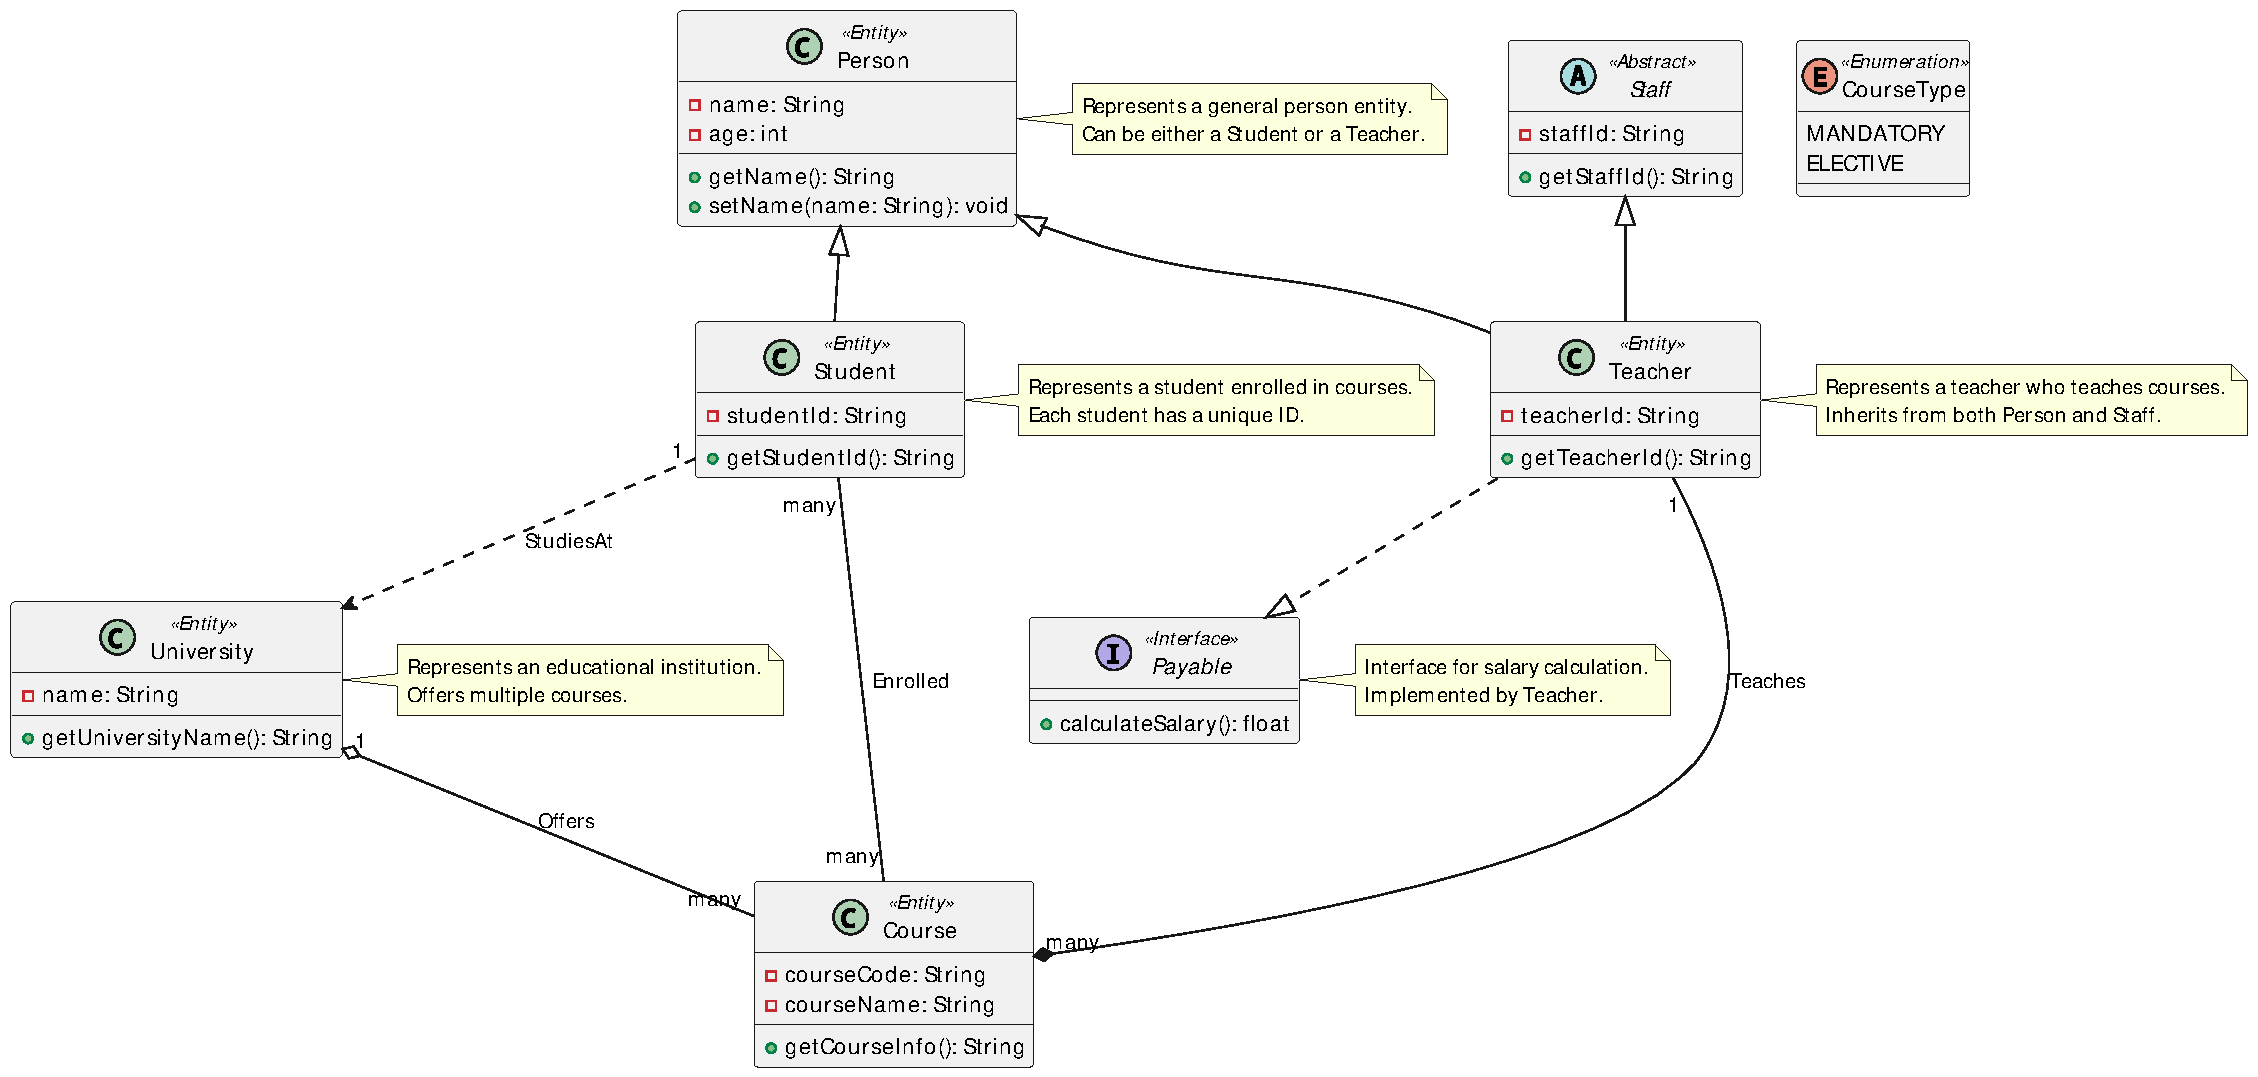
\includegraphics[width=\textwidth]{../figures/out/class_diagram}
	\caption{Class diagram and its features}
	\label{fig:class_diagram}
\end{figure}

\begin{lstlisting}[language=puml, caption={UML class diagram menggunakan PlantUML}]
@startuml
'Define Classes with attributes and methods
class Person <<Entity>> {
	-name: String
	-age: int
	+getName(): String
	+setName(name: String): void
}

class Student <<Entity>> {
	-studentId: String
	+getStudentId(): String
}

class Teacher <<Entity>> {
	-teacherId: String
	+getTeacherId(): String
}

class Course <<Entity>> {
	-courseCode: String
	-courseName: String
	+getCourseInfo(): String
}

class University <<Entity>> {
	-name: String
	+getUniversityName(): String
}

' Abstract Class
abstract class Staff <<Abstract>> {
	-staffId: String
	+getStaffId(): String
}

' Interface
interface Payable <<Interface>> {
	+calculateSalary(): float
}

' Enumeration
enum CourseType <<Enumeration>> {
	MANDATORY
	ELECTIVE
}

' Relationships
Person <|-- Student  
Person <|-- Teacher  
Staff <|-- Teacher   
Teacher ..|> Payable 

University "1" o-- "many" Course  : Offers  
Student "many" -- "many" Course   : Enrolled  
Teacher "1" --* "many" Course    : Teaches  
Student "1" ..> University       : StudiesAt  

' Adding Notes
note right of Person
Represents a general person entity.
Can be either a Student or a Teacher.
end note

note right of Student
Represents a student enrolled in courses.
Each student has a unique ID.
end note

note right of Teacher
Represents a teacher who teaches courses.
Inherits from both Person and Staff.
end note

note right of University
Represents an educational institution.
Offers multiple courses.
end note

note right of Payable
Interface for salary calculation.
Implemented by Teacher.
end note

@enduml
\end{lstlisting}

\subsection{Kelas dan Atribut}
Setiap kelas dalam class diagram direpresentasikan sebagai sebuah kotak yang terdiri dari tiga bagian, yaitu nama kelas, atribut, dan metode. Contoh kelas dalam diagram yang diberikan adalah \texttt{Person}, \texttt{Student}, \texttt{Teacher}, \texttt{Course}, dan \texttt{University}. Atribut dalam kelas ditulis dalam format \texttt{name: type}, seperti berikut:
\begin{lstlisting}[language=puml]
	class Person {
		-name: String
		-age: int
	}
\end{lstlisting}
Simbol \texttt{-} menunjukkan bahwa atribut bersifat \textit{private}, sehingga tidak dapat diakses secara langsung dari luar kelas.

\subsection{Metode dalam Kelas}
Selain atribut, kelas juga memiliki metode yang menunjukkan perilaku atau operasi yang dapat dilakukan oleh objek dari kelas tersebut. Metode dalam UML ditulis dalam format:
\begin{lstlisting}[language=puml]
	+getName(): String
	+setName(name: String): void
\end{lstlisting}
Simbol \texttt{+} menunjukkan bahwa metode bersifat \textit{public}, sehingga dapat diakses dari luar kelas.

\subsection{Hubungan Antar Kelas}
Dalam class diagram, terdapat beberapa jenis hubungan yang menunjukkan keterkaitan antar kelas, yaitu:

\begin{enumerate}
	\item \textbf{Inheritance (Pewarisan)} \\
	Pewarisan dalam UML direpresentasikan dengan panah kosong (\texttt{<|--}) yang menunjukkan bahwa suatu kelas merupakan subclass dari kelas lain. Misalnya, kelas \texttt{Student} dan \texttt{Teacher} mewarisi atribut dan metode dari kelas \texttt{Person}:
	\begin{lstlisting}[language=puml]
		Person <|-- Student  
		Person <|-- Teacher
	\end{lstlisting}
	
	\item \textbf{Association (Asosiasi)} \\
	Asosiasi menunjukkan hubungan antar kelas dalam sistem. Misalnya, hubungan antara \texttt{Student} dan \texttt{Course} dalam diagram menunjukkan bahwa banyak mahasiswa dapat mendaftar ke banyak mata kuliah:
	\begin{lstlisting}[language=puml]
		Student "many" -- "many" Course   : Enrolled
	\end{lstlisting}
	
	\item \textbf{Aggregation (Agregasi)} \\
	Agregasi menunjukkan hubungan "bagian dari" tetapi objek yang dimiliki dapat berdiri sendiri tanpa pemiliknya. Dalam contoh diagram, \texttt{University} memiliki banyak \texttt{Course}, tetapi kursus tetap ada meskipun universitas dihapus:
	\begin{lstlisting}[language=puml]
		University "1" o-- "many" Course  : Offers
	\end{lstlisting}
	
	\item \textbf{Composition (Komposisi)} \\
	Komposisi mirip dengan agregasi, tetapi bagian yang dimiliki tidak dapat berdiri sendiri tanpa pemiliknya. Dalam contoh diagram, \texttt{Teacher} memiliki banyak \texttt{Course}, dan kursus tidak akan ada tanpa pengajar:
	\begin{lstlisting}[language=puml]
		Teacher "1" --* "many" Course    : Teaches
	\end{lstlisting}
	
	\item \textbf{Dependency (Ketergantungan)} \\
	Dependency menunjukkan bahwa suatu kelas bergantung pada kelas lain tetapi tidak memiliki hubungan yang kuat. Misalnya, \texttt{Student} bergantung pada \texttt{University}:
	\begin{lstlisting}[language=puml]
		Student "1" ..> University       : StudiesAt
	\end{lstlisting}
\end{enumerate}

\subsection{Kelas Abstrak dan Interface}
Class diagram juga dapat mencakup kelas abstrak dan antarmuka (\textit{interface}). 

\begin{itemize}
	\item \textbf{Kelas Abstrak} \\
	Kelas abstrak tidak dapat diinstansiasi dan biasanya digunakan sebagai dasar bagi kelas lain. Dalam contoh diagram, \texttt{Staff} merupakan kelas abstrak yang diwarisi oleh \texttt{Teacher}:
	\begin{lstlisting}[language=puml]
		abstract class Staff {
			-staffId: String
			+getStaffId(): String
		}
	\end{lstlisting}
	
	\item \textbf{Interface} \\
	Interface mendefinisikan metode yang harus diimplementasikan oleh kelas yang menggunakannya. Dalam contoh diagram, \texttt{Payable} merupakan interface yang diimplementasikan oleh \texttt{Teacher}:
	\begin{lstlisting}[language=puml]
		interface Payable {
			+calculateSalary(): float
		}
		
		Teacher ..|> Payable
	\end{lstlisting}
\end{itemize}

\subsection{Enumerasi}
Enumerasi (\textit{Enumeration}) adalah tipe data khusus yang berisi sekumpulan nilai tetap. Dalam diagram ini, \texttt{CourseType} adalah enumerasi dengan dua nilai:
\begin{lstlisting}[language=puml]
	enum CourseType {
		MANDATORY
		ELECTIVE
	}
\end{lstlisting}

\subsection{Stereotip}
Stereotip dalam UML digunakan untuk mengklasifikasikan elemen dalam diagram. Dalam contoh diagram, digunakan stereotip seperti berikut:
\begin{itemize}
	\item \texttt{<<Entity>>} untuk kelas seperti \texttt{Person}, \texttt{Student}, dan \texttt{Course}.
	\item \texttt{<<Abstract>>} untuk kelas abstrak \texttt{Staff}.
	\item \texttt{<<Interface>>} untuk antarmuka \texttt{Payable}.
	\item \texttt{<<Enumeration>>} untuk enumerasi \texttt{CourseType}.
\end{itemize}

\subsection{Catatan (Notes)}
Dalam UML, catatan digunakan untuk memberikan informasi tambahan tentang elemen dalam diagram. Misalnya, pada diagram terdapat catatan yang menjelaskan fungsi dari kelas \texttt{Person}:
\begin{lstlisting}[language=puml]
	note right of Person
	Represents a general person entity.
	Can be either a Student or a Teacher.
	end note
\end{lstlisting}

Class diagram adalah alat yang sangat berguna dalam pemodelan perangkat lunak karena memungkinkan pengembang untuk memahami struktur sistem sebelum implementasi. Diagram ini mencakup berbagai elemen seperti kelas, atribut, metode, hubungan antar kelas, serta konsep seperti kelas abstrak, interface, enumerasi, dan catatan untuk dokumentasi tambahan.

\section{Object Diagram}

Object diagram merupakan salah satu diagram struktural dalam Unified Modeling Language (UML) yang digunakan untuk merepresentasikan instance dari kelas pada suatu waktu tertentu. Diagram ini memberikan gambaran bagaimana objek-objek dalam sistem saling berinteraksi dan berhubungan dalam keadaan tertentu.

\begin{figure}[ht]
	\centering
	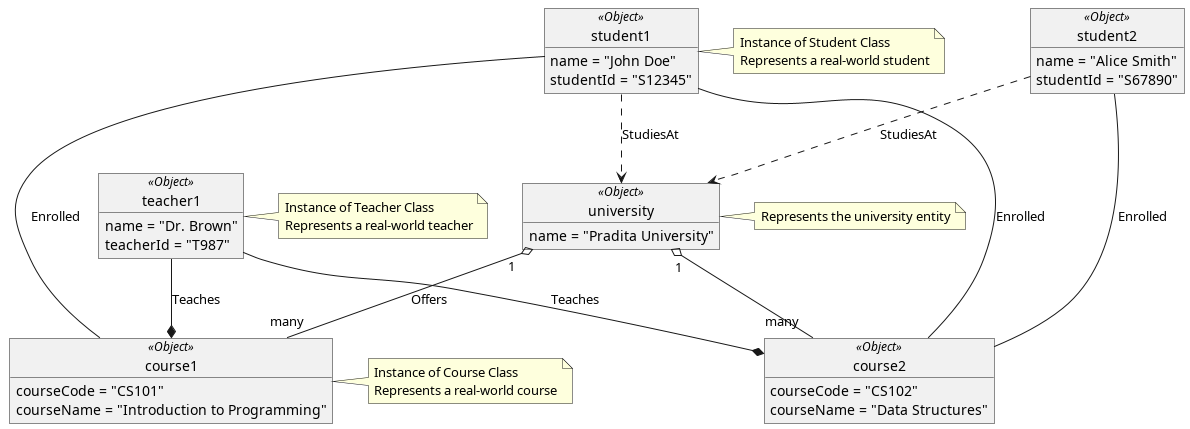
\includegraphics[width=\textwidth]{../figures/out/object_diagram}
	\caption{Object Diagram dan Fitur-fiturnya}
	\label{fig:object_diagram}
\end{figure}

\begin{lstlisting}[language=puml,caption={PlantUML Object Diagram Code}]
	@startuml
	
	' Defining Objects
	object student1 <<Object>> {
		name = "John Doe"
		studentId = "S12345"
	}
	
	object student2 <<Object>> {
		name = "Alice Smith"
		studentId = "S67890"
	}
	
	object course1 <<Object>> {
		courseCode = "CS101"
		courseName = "Introduction to Programming"
	}
	
	object course2 <<Object>> {
		courseCode = "CS102"
		courseName = "Data Structures"
	}
	
	object teacher1 <<Object>> {
		name = "Dr. Brown"
		teacherId = "T987"
	}
	
	object university <<Object>> {
		name = "Pradita University"
	}
	
	' Relationships
	student1 -- course1 : Enrolled
	student1 -- course2 : Enrolled
	student2 -- course2 : Enrolled
	teacher1 --* course1 : Teaches
	teacher1 --* course2 : Teaches
	university "1" o-- "many" course1 : Offers
	university "1" o-- "many" course2
	
	' Dependency Relationship
	student1 ..> university : StudiesAt
	student2 ..> university : StudiesAt
	
	' Notes for explanation
	note right of student1
	Instance of Student Class
	Represents a real-world student
	end note
	
	note right of course1
	Instance of Course Class
	Represents a real-world course
	end note
	
	note right of teacher1
	Instance of Teacher Class
	Represents a real-world teacher
	end note
	
	note right of university
	Represents the university entity
	end note
	
	@enduml
\end{lstlisting}


\subsection{Objek dan Atributnya}
Objek dalam object diagram merepresentasikan instance spesifik dari suatu kelas dalam sistem. Objek dalam UML ditulis dengan format:
\begin{lstlisting}[language=puml]
	object student1 <<Object>> {
		name = "John Doe"
		studentId = "S12345"
	}


\end{lstlisting}
Objek \texttt{student1} adalah instance dari kelas \texttt{Student} dengan nilai atribut spesifik. Setiap objek memiliki nama yang menunjukkan bahwa objek tersebut merupakan realisasi dari suatu kelas.

\subsection{Hubungan Antar Objek}
Seperti dalam class diagram, object diagram juga menggambarkan hubungan antar objek dalam sistem. Beberapa hubungan yang dapat muncul dalam diagram objek antara lain:

\begin{enumerate}
	\item \textbf{Association (Asosiasi)} \\
	Asosiasi menunjukkan hubungan antara dua objek tanpa menunjukkan kepemilikan. Contoh pada diagram adalah hubungan antara \texttt{student1} dan \texttt{course1} yang menunjukkan bahwa mahasiswa terdaftar pada suatu kursus:
	\begin{lstlisting}[language=puml]
		student1 -- course1 : Enrolled
	\end{lstlisting}
	
	\item \textbf{Aggregation (Agregasi)} \\
	Agregasi menunjukkan bahwa satu objek merupakan bagian dari objek lain, tetapi masih dapat berdiri sendiri. Contohnya adalah \texttt{university} yang memiliki banyak \texttt{course}, tetapi kursus tetap bisa ada meskipun universitas tidak ada:
	\begin{lstlisting}[language=puml]
		university "1" o-- "many" course1 : Offers
	\end{lstlisting}
	
	\item \textbf{Composition (Komposisi)} \\
	Komposisi menunjukkan bahwa satu objek tidak dapat berdiri sendiri tanpa objek pemiliknya. Contohnya adalah hubungan antara \texttt{teacher1} dan \texttt{course1}, yang menunjukkan bahwa kursus tidak bisa ada tanpa seorang pengajar:
	\begin{lstlisting}[language=puml]
		teacher1 --* course1 : Teaches
	\end{lstlisting}
	
	\item \textbf{Dependency (Ketergantungan)} \\
	Dependency menunjukkan bahwa satu objek bergantung pada objek lain, tetapi tidak memiliki hubungan yang kuat. Contohnya adalah hubungan antara \texttt{student1} dan \texttt{university}:
	\begin{lstlisting}[language=puml]
		student1 ..> university : StudiesAt
	\end{lstlisting}
\end{enumerate}

\subsection{Stereotip dalam Object Diagram}
Stereotip digunakan untuk memberikan klasifikasi tambahan pada objek dalam diagram UML. Dalam object diagram, digunakan stereotip \texttt{<<Object>>} untuk menandai bahwa elemen tersebut merupakan instance dari suatu kelas:
\begin{lstlisting}[language=puml]
	object student1 <<Object>> {
		name = "John Doe"
		studentId = "S12345"
	}
\end{lstlisting}

\subsection{Catatan (Notes)}
Catatan digunakan untuk memberikan informasi tambahan mengenai suatu elemen dalam object diagram. Contohnya adalah catatan yang menjelaskan objek \texttt{student1}:
\begin{lstlisting}[language=puml]
	note right of student1
	Instance of Student Class
	Represents a real-world student
	end note
\end{lstlisting}
Catatan ini menjelaskan bahwa objek \texttt{student1} adalah instance dari kelas \texttt{Student} dan mewakili seorang mahasiswa nyata dalam sistem.

Object diagram adalah alat yang berguna dalam pemodelan perangkat lunak karena memberikan gambaran bagaimana objek dalam sistem berinteraksi pada suatu titik waktu tertentu. Diagram ini mencakup berbagai elemen seperti objek, atribut, hubungan antar objek, serta konsep seperti asosiasi, agregasi, komposisi, dependency, stereotip, dan catatan untuk dokumentasi tambahan.


\section{Component Diagram}

Component diagram merupakan salah satu diagram struktural dalam Unified Modeling Language (UML) yang digunakan untuk merepresentasikan komponen-komponen dalam suatu sistem perangkat lunak beserta hubungan antar komponen tersebut. Diagram ini berguna untuk memahami bagaimana komponen dalam sistem berinteraksi satu sama lain dan bagaimana layanan-layanan tertentu disediakan dan digunakan.

\begin{figure}[ht]
	\centering
	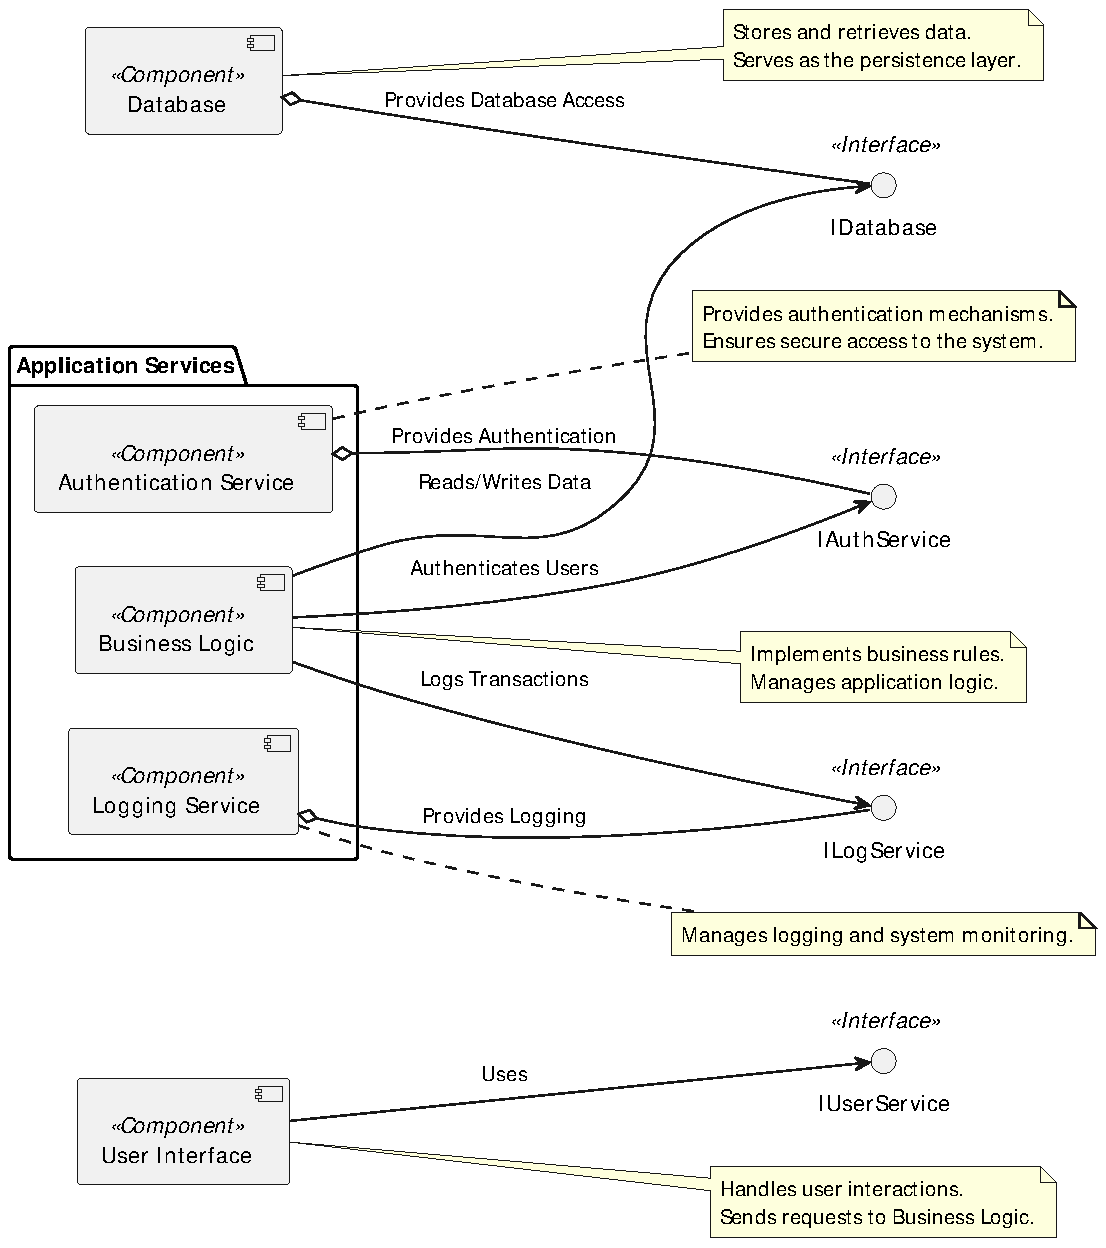
\includegraphics[width=.9\textwidth]{../figures/out/component_diagram}
	\caption{Component Diagram dan Fitur-fiturnya}
	\label{fig:component_diagram}
\end{figure}

\begin{lstlisting}[language=puml,caption={PlantUML Component Diagram Code}]
	@startuml
	
	' Force vertical layout
	left to right direction
	
	' Define components inside the package
	package "Application Services" {
		component "Business Logic" <<Component>> as BL
		component "Authentication Service" <<Component>> as Auth
		component "Logging Service" <<Component>> as Log
	}
	
	' Define other components
	component "User Interface" <<Component>> as UI
	component "Database" <<Component>> as DB
	
	' Define interfaces
	interface "IUserService" <<Interface>> as IUserService
	interface "IDatabase" <<Interface>> as IDatabase
	interface "IAuthService" <<Interface>> as IAuthService
	interface "ILogService" <<Interface>> as ILogService
	
	' Component dependencies
	UI --> IUserService : Uses
	BL --> IDatabase : Reads/Writes Data
	BL --> IAuthService : Authenticates Users
	BL --> ILogService : Logs Transactions
	Auth o-- IAuthService : Provides Authentication
	DB o-- IDatabase : Provides Database Access
	Log o-- ILogService : Provides Logging
	
	' Notes explaining components
	note right of UI
	Handles user interactions.
	Sends requests to Business Logic.
	end note
	
	note right of BL
	Implements business rules.
	Manages application logic.
	end note
	
	note right of DB
	Stores and retrieves data.
	Serves as the persistence layer.
	end note
	
	note right of Auth
	Provides authentication mechanisms.
	Ensures secure access to the system.
	end note
	
	note right of Log
	Manages logging and system monitoring.
	end note
	
	@enduml
\end{lstlisting}


\subsection{Komponen dalam Diagram Komponen}
Komponen dalam UML direpresentasikan sebagai unit mandiri yang memiliki antarmuka dan dapat digunakan kembali. Setiap komponen dalam diagram ini dideklarasikan menggunakan stereotip \texttt{<<Component>>}. Contohnya:
\begin{lstlisting}[language=puml]
	component "User Interface" <<Component>> as UI
	component "Business Logic" <<Component>> as BL
	component "Database" <<Component>> as DB
\end{lstlisting}
Komponen \texttt{User Interface} berfungsi sebagai lapisan interaksi dengan pengguna, sementara \texttt{Business Logic} menangani aturan bisnis, dan \texttt{Database} bertindak sebagai penyimpanan data.

\subsection{Antarmuka dalam Diagram Komponen}
Antarmuka (\textit{interface}) digunakan untuk menentukan layanan yang disediakan atau diperlukan oleh suatu komponen. Antarmuka dalam UML dinyatakan menggunakan stereotip \texttt{<<Interface>>}. Contoh definisi antarmuka:
\begin{lstlisting}[language=puml]
	interface "IUserService" <<Interface>> as IUserService
	interface "IDatabase" <<Interface>> as IDatabase
\end{lstlisting}
Antarmuka ini digunakan untuk mendeklarasikan kontrak layanan yang harus dipenuhi oleh komponen.

\subsection{Hubungan Antar Komponen}
Diagram komponen menunjukkan berbagai hubungan antara komponen dalam sistem. Beberapa jenis hubungan yang umum digunakan dalam diagram ini meliputi:

\begin{enumerate}
	\item \textbf{Dependency (Ketergantungan)} \\
	Ketergantungan menunjukkan bahwa satu komponen menggunakan layanan dari komponen lain. Dalam contoh berikut, \texttt{User Interface} bergantung pada layanan \texttt{IUserService}:
	\begin{lstlisting}[language=puml]
		UI --> IUserService : Uses
	\end{lstlisting}
	
	\item \textbf{Provided Interface (Antarmuka yang Disediakan)} \\
	Komponen yang menyediakan layanan akan menunjukkan antarmuka yang disediakannya menggunakan simbol \texttt{o--}. Contohnya, komponen \texttt{Database} menyediakan layanan \texttt{IDatabase}:
	\begin{lstlisting}[language=puml]
		DB o-- IDatabase : Provides Database Access
	\end{lstlisting}
	
	\item \textbf{Required Interface (Antarmuka yang Dibutuhkan)} \\
	Komponen yang membutuhkan layanan dari komponen lain akan menggunakan simbol \texttt{-->}. Contoh berikut menunjukkan bahwa komponen \texttt{Business Logic} memerlukan layanan dari \texttt{IDatabase}:
	\begin{lstlisting}[language=puml]
		BL --> IDatabase : Reads/Writes Data
	\end{lstlisting}
\end{enumerate}

\subsection{Pengelompokan Komponen dengan Paket}
Dalam sistem besar, komponen dapat dikelompokkan ke dalam paket untuk menunjukkan bagian-bagian modular dari sistem. Dalam diagram ini, beberapa komponen dikelompokkan ke dalam paket \texttt{Application Services}:
\begin{lstlisting}[language=puml]
	package "Application Services" {
		component "Business Logic" <<Component>> as BL
		component "Authentication Service" <<Component>> as Auth
		component "Logging Service" <<Component>> as Log
	}
\end{lstlisting}
Pengelompokan ini membantu dalam memahami arsitektur sistem secara lebih terstruktur.

\subsection{Catatan (Notes) dalam Diagram Komponen}
Catatan digunakan untuk memberikan informasi tambahan mengenai suatu komponen atau hubungan antar komponen dalam diagram. Misalnya, berikut adalah catatan yang menjelaskan fungsi dari komponen \texttt{User Interface}:
\begin{lstlisting}[language=puml]
	note right of UI
	Handles user interactions.
	Sends requests to Business Logic.
	end note
\end{lstlisting}
Catatan ini membantu menjelaskan peran setiap komponen dalam sistem secara lebih rinci.


Component diagram adalah alat yang sangat berguna dalam pemodelan perangkat lunak karena memungkinkan desainer untuk memahami bagaimana komponen dalam sistem berinteraksi satu sama lain. Diagram ini mencakup berbagai elemen seperti komponen, antarmuka, hubungan antar komponen, pengelompokan dalam paket, serta catatan untuk dokumentasi tambahan.


\section{Deployment Diagram dan Fitur-fiturnya}

Deployment Diagram merupakan salah satu diagram dalam Unified Modeling Language (UML) yang digunakan untuk memodelkan arsitektur fisik dari sistem perangkat lunak. Diagram ini menunjukkan bagaimana komponen perangkat lunak dipetakan ke perangkat keras serta bagaimana komunikasi antara berbagai elemen dilakukan.

\begin{figure}[ht]
	\centering
	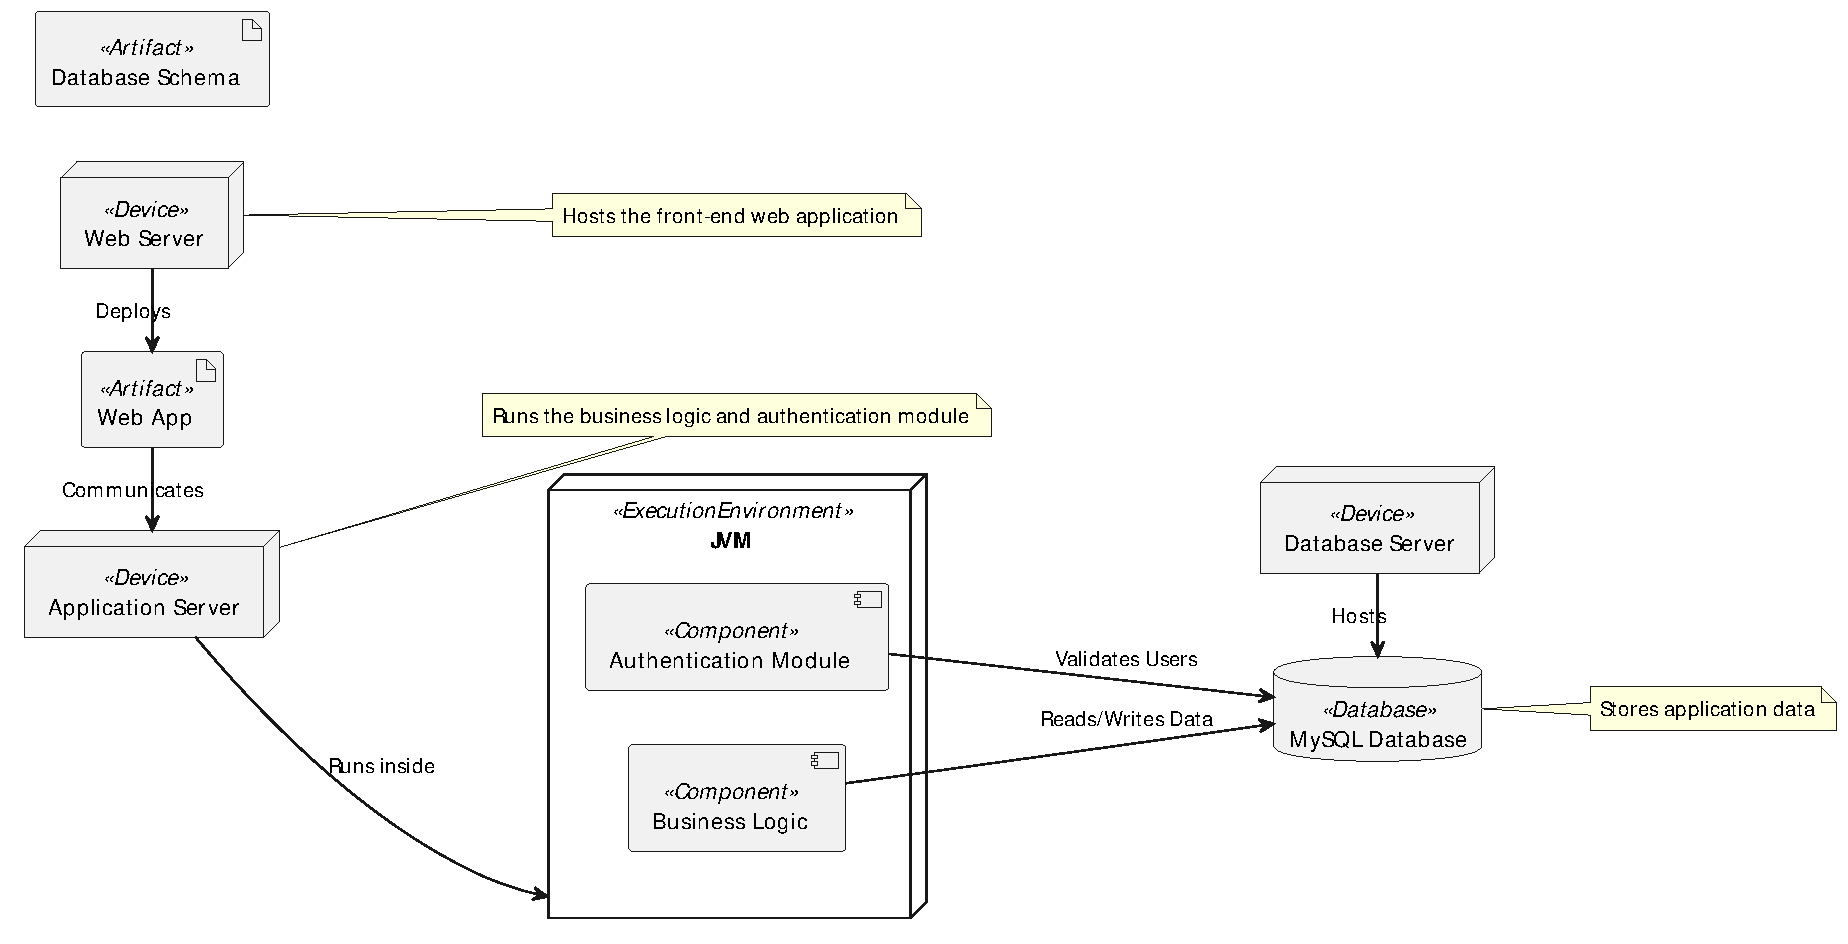
\includegraphics[width=\textwidth]{../figures/out/deployment_diagram}
	\caption{Deployment Diagram dan Fitur-fiturnya}
	\label{fig:deployment_diagram}
\end{figure}



\subsection{Node dalam Deployment Diagram}
Node (\textit{simpul}) adalah elemen utama dalam deployment diagram yang merepresentasikan perangkat keras atau lingkungan eksekusi yang digunakan untuk menjalankan komponen perangkat lunak. Node dalam UML dapat memiliki stereotip seperti \texttt{<<Device>>} dan \texttt{<<ExecutionEnvironment>>}.

\begin{lstlisting}[language=puml,caption={Contoh Definisi Node dalam Deployment Diagram}]
	node "Web Server" <<Device>> as WebServer
	node "Application Server" <<Device>> as AppServer
	node "Database Server" <<Device>> as DBServer
\end{lstlisting}
Dalam contoh di atas, terdapat tiga node utama yang mewakili server tempat sistem dijalankan, yaitu Web Server, Application Server, dan Database Server.

\subsection{Lingkungan Eksekusi (Execution Environment)}
Lingkungan eksekusi (\textit{Execution Environment}) digunakan untuk merepresentasikan platform perangkat lunak tempat komponen dijalankan, seperti JVM (Java Virtual Machine), container Docker, atau runtime lainnya.

\begin{lstlisting}[language=puml,caption={Contoh Execution Environment dalam Deployment Diagram}]
	node "JVM" <<ExecutionEnvironment>> as JVM {
		component "Business Logic" <<Component>> as BL
		component "Authentication Module" <<Component>> as Auth
	}
\end{lstlisting}
Dalam contoh di atas, lingkungan eksekusi \texttt{JVM} berada di dalam \texttt{Application Server} dan digunakan untuk menjalankan komponen seperti \texttt{Business Logic} dan \texttt{Authentication Module}.

\subsection{Artefak dalam Deployment Diagram}
Artefak (\textit{Artifact}) dalam deployment diagram merepresentasikan entitas fisik dari perangkat lunak, seperti file aplikasi web, database schema, atau pustaka perangkat lunak yang di-deploy.

\begin{lstlisting}[language=puml,caption={Contoh Artefak dalam Deployment Diagram}]
	artifact "Web App" <<Artifact>> as WebApp
	artifact "Database Schema" <<Artifact>> as DBSchema
\end{lstlisting}
Pada contoh di atas, terdapat dua artefak: \texttt{Web App}, yang merepresentasikan aplikasi web yang dijalankan di server, dan \texttt{Database Schema}, yang merepresentasikan skema database.

\subsection{Database dalam Deployment Diagram}
Deployment diagram juga dapat menyertakan elemen \texttt{<<Database>>} untuk menunjukkan sistem penyimpanan data yang digunakan dalam arsitektur perangkat lunak.

\begin{lstlisting}[language=puml,caption={Contoh Database dalam Deployment Diagram}]
	database "MySQL Database" <<Database>> as MySQLDB
\end{lstlisting}
Dalam diagram ini, \texttt{MySQL Database} berfungsi sebagai penyimpanan utama untuk aplikasi.

\subsection{Hubungan Antar Komponen dalam Deployment Diagram}
Deployment diagram mendukung beberapa jenis hubungan antar elemen, termasuk:

\begin{itemize}
	\item \textbf{Deployment (Pendeployan)} \\
	Menunjukkan bahwa suatu artefak dideploy ke dalam suatu node.
	\begin{lstlisting}[language=puml]
		WebServer -right-> WebApp : Deploys
	\end{lstlisting}
	
	\item \textbf{Communication (Komunikasi)} \\
	Menunjukkan bagaimana komponen berkomunikasi satu sama lain.
	\begin{lstlisting}[language=puml]
		WebApp -right-> AppServer : Communicates
	\end{lstlisting}
	
	\item \textbf{Hosting (Hosting)} \\
	Menunjukkan bahwa suatu komponen berjalan di dalam suatu lingkungan eksekusi.
	\begin{lstlisting}[language=puml]
		AppServer -down-> JVM : Runs inside
	\end{lstlisting}
\end{itemize}

\subsection{Catatan (Notes) dalam Deployment Diagram}
Deployment diagram sering menyertakan catatan untuk memberikan penjelasan tambahan mengenai elemen diagram.

\begin{lstlisting}[language=puml,caption={Contoh Catatan dalam Deployment Diagram}]
	note right of WebServer
	Hosts the front-end web application
	end note
\end{lstlisting}

Catatan ini membantu dalam memberikan deskripsi yang lebih jelas mengenai peran masing-masing komponen dalam diagram.

Deployment diagram adalah alat penting dalam rekayasa perangkat lunak yang memungkinkan pengembang untuk memahami bagaimana sistem diimplementasikan pada infrastruktur fisik. Diagram ini mencakup elemen-elemen seperti node (\textit{device, execution environment}), artefak, database, serta berbagai jenis hubungan seperti \textit{deployment}, \textit{communication}, dan \textit{hosting}. 

\section{Referensi}
Untuk pembelajaran lebih mendalam mengenai UML, silahkan kunjungi tautan berikut: \url{https://www.uml-diagrams.org/}.



	\chapter{Unified Modeling Language: Behavioral Diagram}

\section{Pendahuluan}


\section{Behavioral Diagram}

Behavioral diagram merupakan jenis diagram dalam Unified Modeling Language (UML) yang digunakan untuk merepresentasikan dinamika dan interaksi dalam suatu sistem perangkat lunak. Diagram ini menggambarkan bagaimana komponen dalam sistem beroperasi, bagaimana aliran data atau informasi terjadi, serta bagaimana objek berinteraksi satu sama lain selama eksekusi. Behavioral diagram sangat berguna dalam memahami alur kerja sistem sebelum implementasi, terutama dalam konteks analisis kebutuhan dan desain perangkat lunak.

Terdapat beberapa jenis behavioral diagram dalam UML, termasuk sequence diagram, activity diagram, state machine diagram, dan use case diagram. Masing-masing diagram memiliki peran yang berbeda dalam mendokumentasikan perilaku sistem.


\section{Activity Diagram}

Activity diagram merupakan salah satu diagram perilaku dalam Unified Modeling Language (UML) yang digunakan untuk merepresentasikan aliran proses dalam suatu sistem perangkat lunak. Diagram ini menggambarkan langkah-langkah yang dilakukan dalam sistem, termasuk percabangan, perulangan, eksekusi paralel, serta penanganan kesalahan. Berikut adalah fitur-fitur utama dalam activity diagram:


\begin{figure}
		\centering
		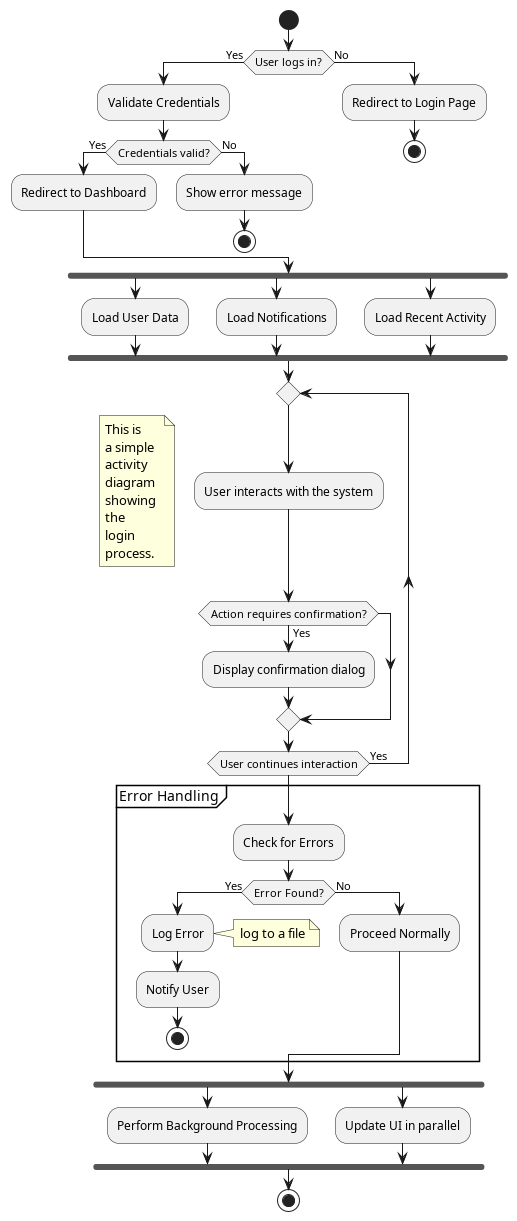
\includegraphics[width=\textwidth,height=\textheight,keepaspectratio]{../figures/out/activity_diagram}
		\caption{Activity diagram and its features}
		\label{fig:activity_diagram}
\end{figure}

\begin{lstlisting}[language=puml, caption=PlantUML code for the activity diagram.]
@startuml

start

' Decision Node
if (User logs in?) then (Yes)
:Validate Credentials;
if (Credentials valid?) then (Yes)
:Redirect to Dashboard;
else (No)
:Show error message;
stop
endif
else (No)
:Redirect to Login Page;
stop
endif

' Fork Node - Parallel Execution
fork
:Load User Data;
fork again
:Load Notifications;
fork again
:Load Recent Activity;
end fork

' Looping Construct
repeat
:User interacts with the system;
floating note left
This is 
a simple 
activity 
diagram
showing 
the 
login 
process.
end note
if (Action requires confirmation?) then (Yes)
:Display confirmation dialog;
endif
repeat while (User continues interaction) is (Yes)

' Exception Handling
partition "Error Handling" {
	:Check for Errors;
	if (Error Found?) then (Yes)
	:Log Error;
	' Notes explaining components
	note right
	log to a file
	end note
	:Notify User;
	stop
	else (No)
	:Proceed Normally;
	endif
}

' Synchronization and Merging Flows
fork
:Perform Background Processing;
fork again
:Update UI in parallel;
end fork

' Final Node
stop

@enduml
\end{lstlisting}


\subsection{Alur Masuk dan Keputusan}
Activity diagram dimulai dengan \textit{start node} yang merepresentasikan awal proses sistem. Langkah pertama dalam diagram ini adalah memeriksa apakah pengguna sudah masuk (\texttt{User logs in?}). Jika ya, sistem akan memvalidasi kredensial pengguna:

\begin{lstlisting}[language=puml]
	if (User logs in?) then (Yes)
	:Validate Credentials;
	if (Credentials valid?) then (Yes)
	:Redirect to Dashboard;
	else (No)
	:Show error message;
	stop
	endif
	else (No)
	:Redirect to Login Page;
	stop
	endif
\end{lstlisting}

Jika kredensial valid, pengguna akan diarahkan ke halaman dashboard. Jika tidak valid, sistem menampilkan pesan kesalahan dan menghentikan eksekusi. Jika pengguna tidak masuk, sistem akan mengarahkannya ke halaman login.

\subsection{Eksekusi Paralel}
Activity diagram mendukung eksekusi paralel menggunakan \textit{fork node}. Hal ini memungkinkan beberapa aktivitas dijalankan bersamaan sebelum akhirnya disinkronisasi kembali. Dalam diagram ini, setelah pengguna berhasil masuk, sistem akan memuat data pengguna, notifikasi, dan aktivitas terbaru secara paralel:

\begin{lstlisting}[language=puml]
	fork
	:Load User Data;
	fork again
	:Load Notifications;
	fork again
	:Load Recent Activity;
	end fork
\end{lstlisting}

Proses ini meningkatkan efisiensi karena sistem dapat menangani beberapa tugas sekaligus.

\subsection{Perulangan}
Perulangan dalam activity diagram direpresentasikan menggunakan struktur \texttt{repeat}, yang memungkinkan sistem untuk mengulang suatu aktivitas hingga kondisi tertentu tidak lagi terpenuhi. Contoh dalam diagram adalah interaksi pengguna dengan sistem yang dapat berulang selama pengguna masih aktif:

\begin{lstlisting}[language=puml]
	repeat
	:User interacts with the system;
	floating note left
	This is 
	a simple 
	activity 
	diagram
	showing 
	the 
	login 
	process.
	end note
	if (Action requires confirmation?) then (Yes)
	:Display confirmation dialog;
	endif
	repeat while (User continues interaction) is (Yes)
\end{lstlisting}

Pengguna dapat terus berinteraksi dengan sistem hingga mereka berhenti menggunakan aplikasi.

\subsection{Penanganan Kesalahan}
Activity diagram juga dapat merepresentasikan mekanisme penanganan kesalahan (\textit{error handling}). Dalam contoh diagram, jika terjadi kesalahan, sistem akan mencatat log kesalahan dan memberi tahu pengguna:

\begin{lstlisting}[language=puml]
	partition "Error Handling" {
		:Check for Errors;
		if (Error Found?) then (Yes)
		:Log Error;
		note right
		log to a file
		end note
		:Notify User;
		stop
		else (No)
		:Proceed Normally;
		endif
	}
\end{lstlisting}

Sistem memeriksa apakah ada kesalahan. Jika ada, sistem mencatatnya dalam log dan memberi tahu pengguna sebelum menghentikan proses.

\subsection{Sinkronisasi dan Penggabungan Aliran}
Selain eksekusi paralel, activity diagram mendukung \textit{join node} untuk menyinkronisasi aktivitas yang berjalan bersamaan. Dalam contoh diagram, setelah proses latar belakang selesai, sistem memperbarui UI:

\begin{lstlisting}[language=puml]
	fork
	:Perform Background Processing;
	fork again
	:Update UI in parallel;
	end fork
\end{lstlisting}

Hal ini memastikan bahwa pemrosesan berjalan secara efisien tanpa mengganggu tampilan antarmuka pengguna.

\subsection{Node Awal dan Akhir}
Activity diagram selalu memiliki titik awal (\textit{start node}) dan titik akhir (\textit{stop node}) untuk menandai awal dan akhir dari proses. Pada diagram ini, alur dimulai dengan:

\begin{lstlisting}[language=puml]
	start
\end{lstlisting}

Dan berakhir dengan:

\begin{lstlisting}[language=puml]
	stop
\end{lstlisting}

\subsection{Catatan dalam Diagram}
Dalam UML, catatan (\textit{notes}) digunakan untuk memberikan informasi tambahan tentang elemen dalam diagram. Contoh catatan dalam diagram adalah:

\begin{lstlisting}[language=puml]
	floating note left
	This is 
	a simple 
	activity 
	diagram
	showing 
	the 
	login 
	process.
	end note
\end{lstlisting}

Catatan ini memberikan konteks bagi pembaca untuk memahami bagaimana proses login bekerja dalam sistem.

Activity diagram sangat berguna dalam pemodelan perangkat lunak karena memungkinkan pengembang memahami alur eksekusi sistem sebelum implementasi. Diagram ini mencakup berbagai elemen seperti aktivitas, keputusan, eksekusi paralel, perulangan, penanganan kesalahan, serta catatan tambahan untuk dokumentasi yang lebih jelas.


\section{Sequence Diagram}

Sequence diagram merupakan salah satu diagram perilaku dalam Unified Modeling Language (UML) yang digunakan untuk memodelkan interaksi antar objek dalam suatu sistem secara berurutan. Diagram ini menggambarkan bagaimana pesan dikirim dan diterima antar partisipan dalam suatu skenario tertentu. Sequence diagram sangat berguna dalam memahami bagaimana suatu fitur atau proses bekerja secara detail dengan memperlihatkan alur komunikasi antar komponen dalam sistem. Berikut adalah fitur-fitur utama dalam sequence diagram.

\begin{figure}
	\centering
	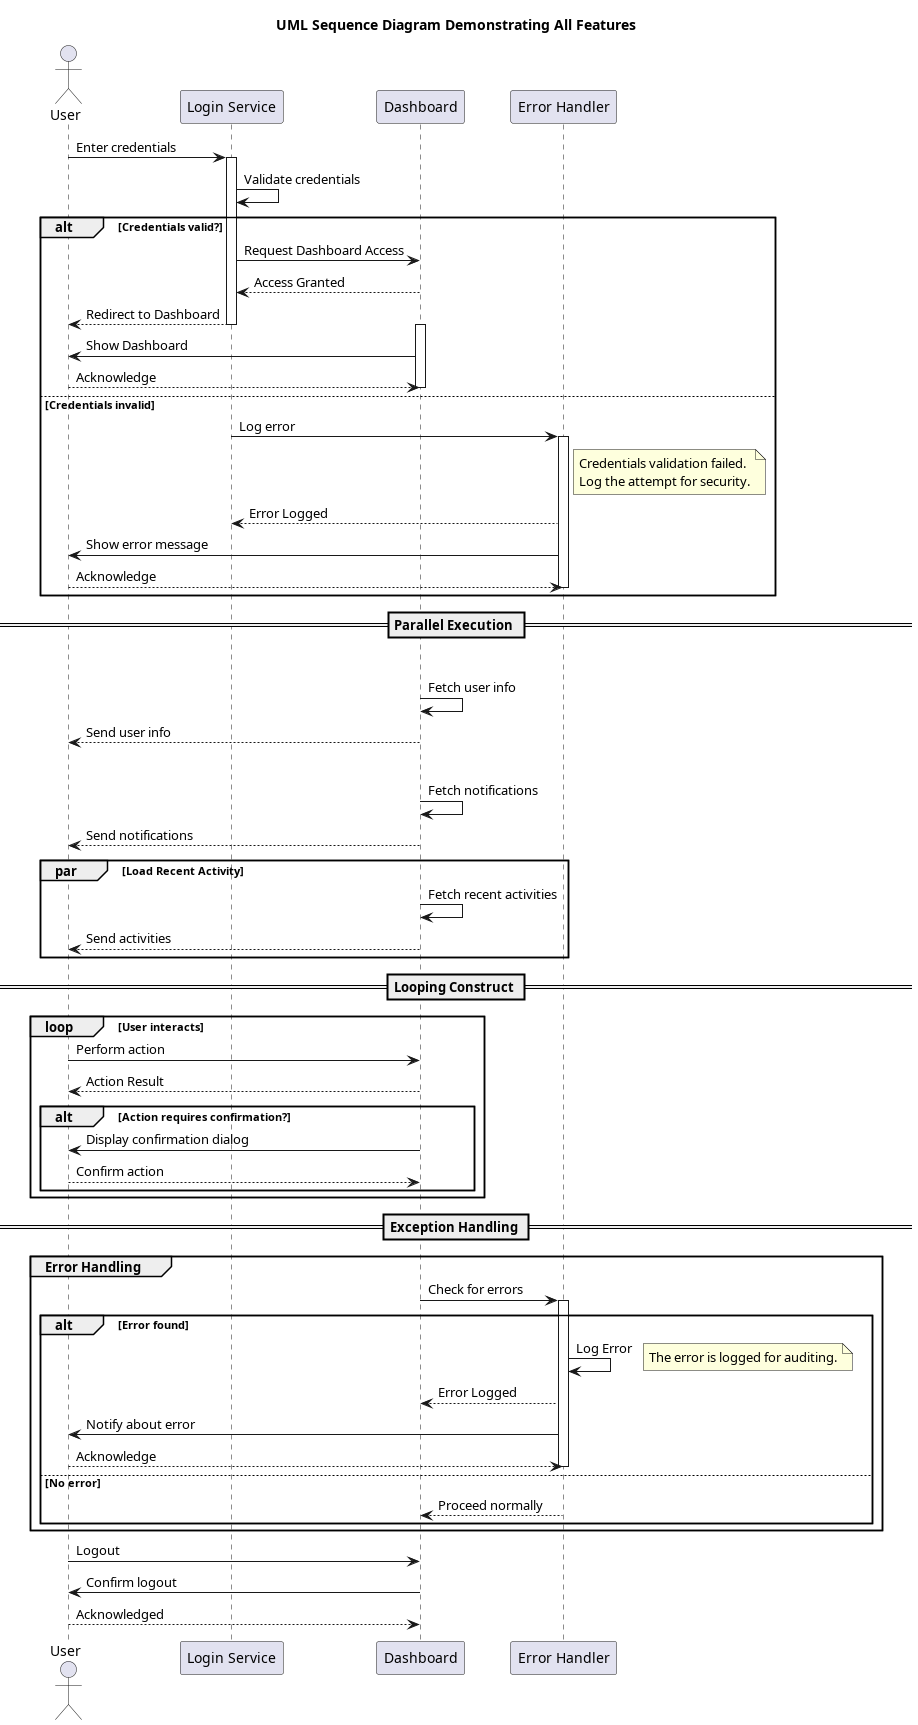
\includegraphics[width=\textwidth,height=\textheight,keepaspectratio]{../figures/out/sequence_diagram}
	\caption{Sequence diagram and its features}
	\label{fig:sequence_diagram}
\end{figure}

\begin{lstlisting}[language=puml, caption=PlantUML code for the sequence diagram.]
@startuml
title UML Sequence Diagram Demonstrating All Features

actor User
participant "Login Service" as LS
participant "Dashboard" as DB
participant "Error Handler" as EH

User -> LS: Enter credentials
activate LS
LS -> LS: Validate credentials

alt Credentials valid?
LS -> DB: Request Dashboard Access
DB --> LS: Access Granted
LS --> User: Redirect to Dashboard
deactivate LS
else Credentials invalid
LS -> EH: Log error
activate EH
note right of EH
Credentials validation failed.
Log the attempt for security.
end note
EH --> LS: Error Logged
EH -> User: Show error message
User --> EH: Acknowledge
deactivate EH
deactivate LS
end alt

== Parallel Execution ==
par Load User Data
DB -> DB: Fetch user info
DB --> User: Send user info
par Load Notifications
DB -> DB: Fetch notifications
DB --> User: Send notifications
par Load Recent Activity
DB -> DB: Fetch recent activities
DB --> User: Send activities
end par

== Looping Construct ==
loop User interacts
User -> DB: Perform action
DB --> User: Action Result
alt Action requires confirmation?
DB -> User: Display confirmation dialog
User --> DB: Confirm action
end alt
end loop

== Exception Handling ==
group Error Handling
DB -> EH: Check for errors
activate EH
alt Error found
EH -> EH: Log Error
note right
The error is logged for auditing.
end note
EH --> DB: Error Logged
EH -> User: Notify about error
User --> EH: Acknowledge
deactivate EH
else No error
EH --> DB: Proceed normally
end alt
end group

User -> DB: Logout
DB -> User: Confirm logout
User --> DB: Acknowledged
deactivate DB

@enduml
\end{lstlisting}

\subsection{Aktor dan Partisipan}
Aktor dan partisipan dalam sequence diagram merepresentasikan entitas yang terlibat dalam interaksi sistem. Aktor biasanya merupakan pengguna atau sistem eksternal, sedangkan partisipan adalah komponen internal yang menerima dan mengirim pesan. Dalam contoh diagram ini, terdapat aktor \texttt{User} yang berinteraksi dengan beberapa partisipan, yaitu \texttt{Login Service}, \texttt{Dashboard}, dan \texttt{Error Handler}.

Deklarasi aktor dan partisipan dalam PlantUML dilakukan menggunakan sintaks berikut:
\begin{lstlisting}[language=puml]
	actor User
	participant "Login Service" as LS
	participant "Dashboard" as DB
	participant "Error Handler" as EH
\end{lstlisting}
Aktor dan partisipan ini menentukan siapa yang akan mengirim dan menerima pesan dalam diagram.

\subsection{Pengiriman Pesan}
Pesan dalam sequence diagram merepresentasikan komunikasi antara partisipan. Terdapat dua jenis pesan yang digunakan dalam diagram ini. Pesan sinkron menggunakan panah solid (\texttt{->}) yang menunjukkan bahwa pemanggil harus menunggu respons sebelum melanjutkan eksekusi. Pesan balik direpresentasikan dengan panah putus-putus (\texttt{-->}), menandakan bahwa suatu partisipan mengembalikan hasil pemrosesan kepada pemanggil.

Pada awal interaksi, pengguna mengirimkan kredensial login ke \texttt{Login Service} untuk divalidasi. Jika kredensial valid, layanan ini akan mengirim permintaan akses ke \texttt{Dashboard}, dan setelah menerima respons, pengguna akan diarahkan ke tampilan utama. Jika kredensial tidak valid, sistem akan mencatat kesalahan dan menampilkan pesan peringatan kepada pengguna.

\begin{lstlisting}[language=puml]
	User -> LS: Enter credentials
	LS -> LS: Validate credentials
	LS -> DB: Request Dashboard Access
	DB --> LS: Access Granted
	LS --> User: Redirect to Dashboard
\end{lstlisting}

\subsection{Aktivasi dan Deaktivasi}
Aktivasi dalam sequence diagram menunjukkan bahwa suatu objek sedang menjalankan suatu proses. Aktivasi terjadi setelah objek menerima pesan dan akan bertahan hingga objek menyelesaikan tugasnya. Aktivasi ditandai dengan perintah \texttt{activate} untuk menunjukkan bahwa suatu partisipan sedang aktif menjalankan suatu proses, dan \texttt{deactivate} untuk menandakan bahwa partisipan telah menyelesaikan tugasnya.

Dalam contoh diagram ini, \texttt{Login Service} diaktifkan ketika menerima permintaan login dan tetap aktif selama memvalidasi kredensial. Setelah proses selesai, partisipan ini dinonaktifkan.

\begin{lstlisting}[language=puml]
	activate LS
	LS -> LS: Validate credentials
	deactivate LS
\end{lstlisting}

\subsection{Percabangan (\texttt{alt})}
PlantUML menyediakan blok \texttt{alt} untuk menangani percabangan dalam suatu alur proses. Percabangan ini digunakan untuk merepresentasikan keputusan dalam sistem, seperti validasi kredensial pengguna.

Dalam contoh diagram ini, jika kredensial valid, sistem akan mengarahkan pengguna ke \texttt{Dashboard}. Sebaliknya, jika kredensial tidak valid, sistem akan mencatat kesalahan dan menampilkan pesan kesalahan.

\begin{lstlisting}[language=puml]
	alt Credentials valid?
	LS -> DB: Request Dashboard Access
	DB --> LS: Access Granted
	LS --> User: Redirect to Dashboard
	else Credentials invalid
	LS -> EH: Log error
	EH --> LS: Error Logged
	EH -> User: Show error message
	User --> EH: Acknowledge
	end alt
\end{lstlisting}

\subsection{Eksekusi Paralel (\texttt{par})}
Sequence diagram juga mendukung eksekusi paralel dengan menggunakan blok \texttt{par}. Dalam contoh diagram ini, setelah pengguna berhasil login, sistem memuat beberapa informasi secara bersamaan, termasuk data pengguna, notifikasi, dan aktivitas terbaru. Masing-masing tugas ini berjalan secara independen tanpa saling menunggu.

\begin{lstlisting}[language=puml]
	par Load User Data
	DB -> DB: Fetch user info
	DB --> User: Send user info
	par Load Notifications
	DB -> DB: Fetch notifications
	DB --> User: Send notifications
	par Load Recent Activity
	DB -> DB: Fetch recent activities
	DB --> User: Send activities
	end par
\end{lstlisting}

\subsection{Perulangan (\texttt{loop})}
PlantUML menyediakan blok \texttt{loop} untuk merepresentasikan aktivitas yang berulang. Dalam contoh diagram ini, pengguna dapat terus berinteraksi dengan sistem selama sesi masih aktif. Jika suatu aksi memerlukan konfirmasi, sistem akan meminta pengguna untuk mengonfirmasi tindakan tersebut sebelum melanjutkan.

\begin{lstlisting}[language=puml]
	loop User interacts
	User -> DB: Perform action
	DB --> User: Action Result
	alt Action requires confirmation?
	DB -> User: Display confirmation dialog
	User --> DB: Confirm action
	end alt
	end loop
\end{lstlisting}

\subsection{Penanganan Kesalahan (\texttt{group})}
PlantUML mendukung mekanisme penanganan kesalahan menggunakan blok \texttt{group}. Dalam contoh ini, jika terjadi kesalahan selama interaksi dengan sistem, layanan akan mencatat kesalahan dan memberikan notifikasi kepada pengguna.

\begin{lstlisting}[language=puml]
	group Error Handling
	DB -> EH: Check for errors
	activate EH
	alt Error found
	EH -> EH: Log Error
	EH --> DB: Error Logged
	EH -> User: Notify about error
	User --> EH: Acknowledge
	deactivate EH
	else No error
	EH --> DB: Proceed normally
	end alt
	end group
\end{lstlisting}

\subsection{Akhir Interaksi dan Logout}
Sequence diagram juga mencakup proses logout, yang menunjukkan bagaimana pengguna mengakhiri sesi. Setelah logout, sistem akan mengonfirmasi bahwa pengguna telah keluar sebelum mengakhiri interaksi.

\begin{lstlisting}[language=puml]
	User -> DB: Logout
	DB -> User: Confirm logout
	User --> DB: Acknowledged
\end{lstlisting}

Sequence diagram dalam UML sangat berguna untuk memodelkan interaksi antara komponen dalam sistem perangkat lunak. Diagram ini merepresentasikan bagaimana pesan dikirim dan diterima dalam suatu alur proses dengan menampilkan aktor, partisipan, pesan sinkron dan balik, aktivasi, percabangan, eksekusi paralel, perulangan, serta penanganan kesalahan. Dengan menggunakan sequence diagram, pengembang dapat memahami bagaimana sistem bekerja sebelum implementasi dilakukan.



\section{Statechart Diagram}

Statechart diagram merupakan salah satu diagram perilaku dalam Unified Modeling Language (UML) yang digunakan untuk merepresentasikan transisi antara berbagai keadaan (state) dalam suatu sistem. Diagram ini menggambarkan bagaimana sistem berubah dari satu keadaan ke keadaan lain sebagai respons terhadap suatu peristiwa (event) atau kondisi tertentu. Statechart diagram sangat berguna dalam model sistem yang memiliki banyak perubahan status, seperti proses pemesanan dalam e-commerce.

\begin{figure}
	\centering
	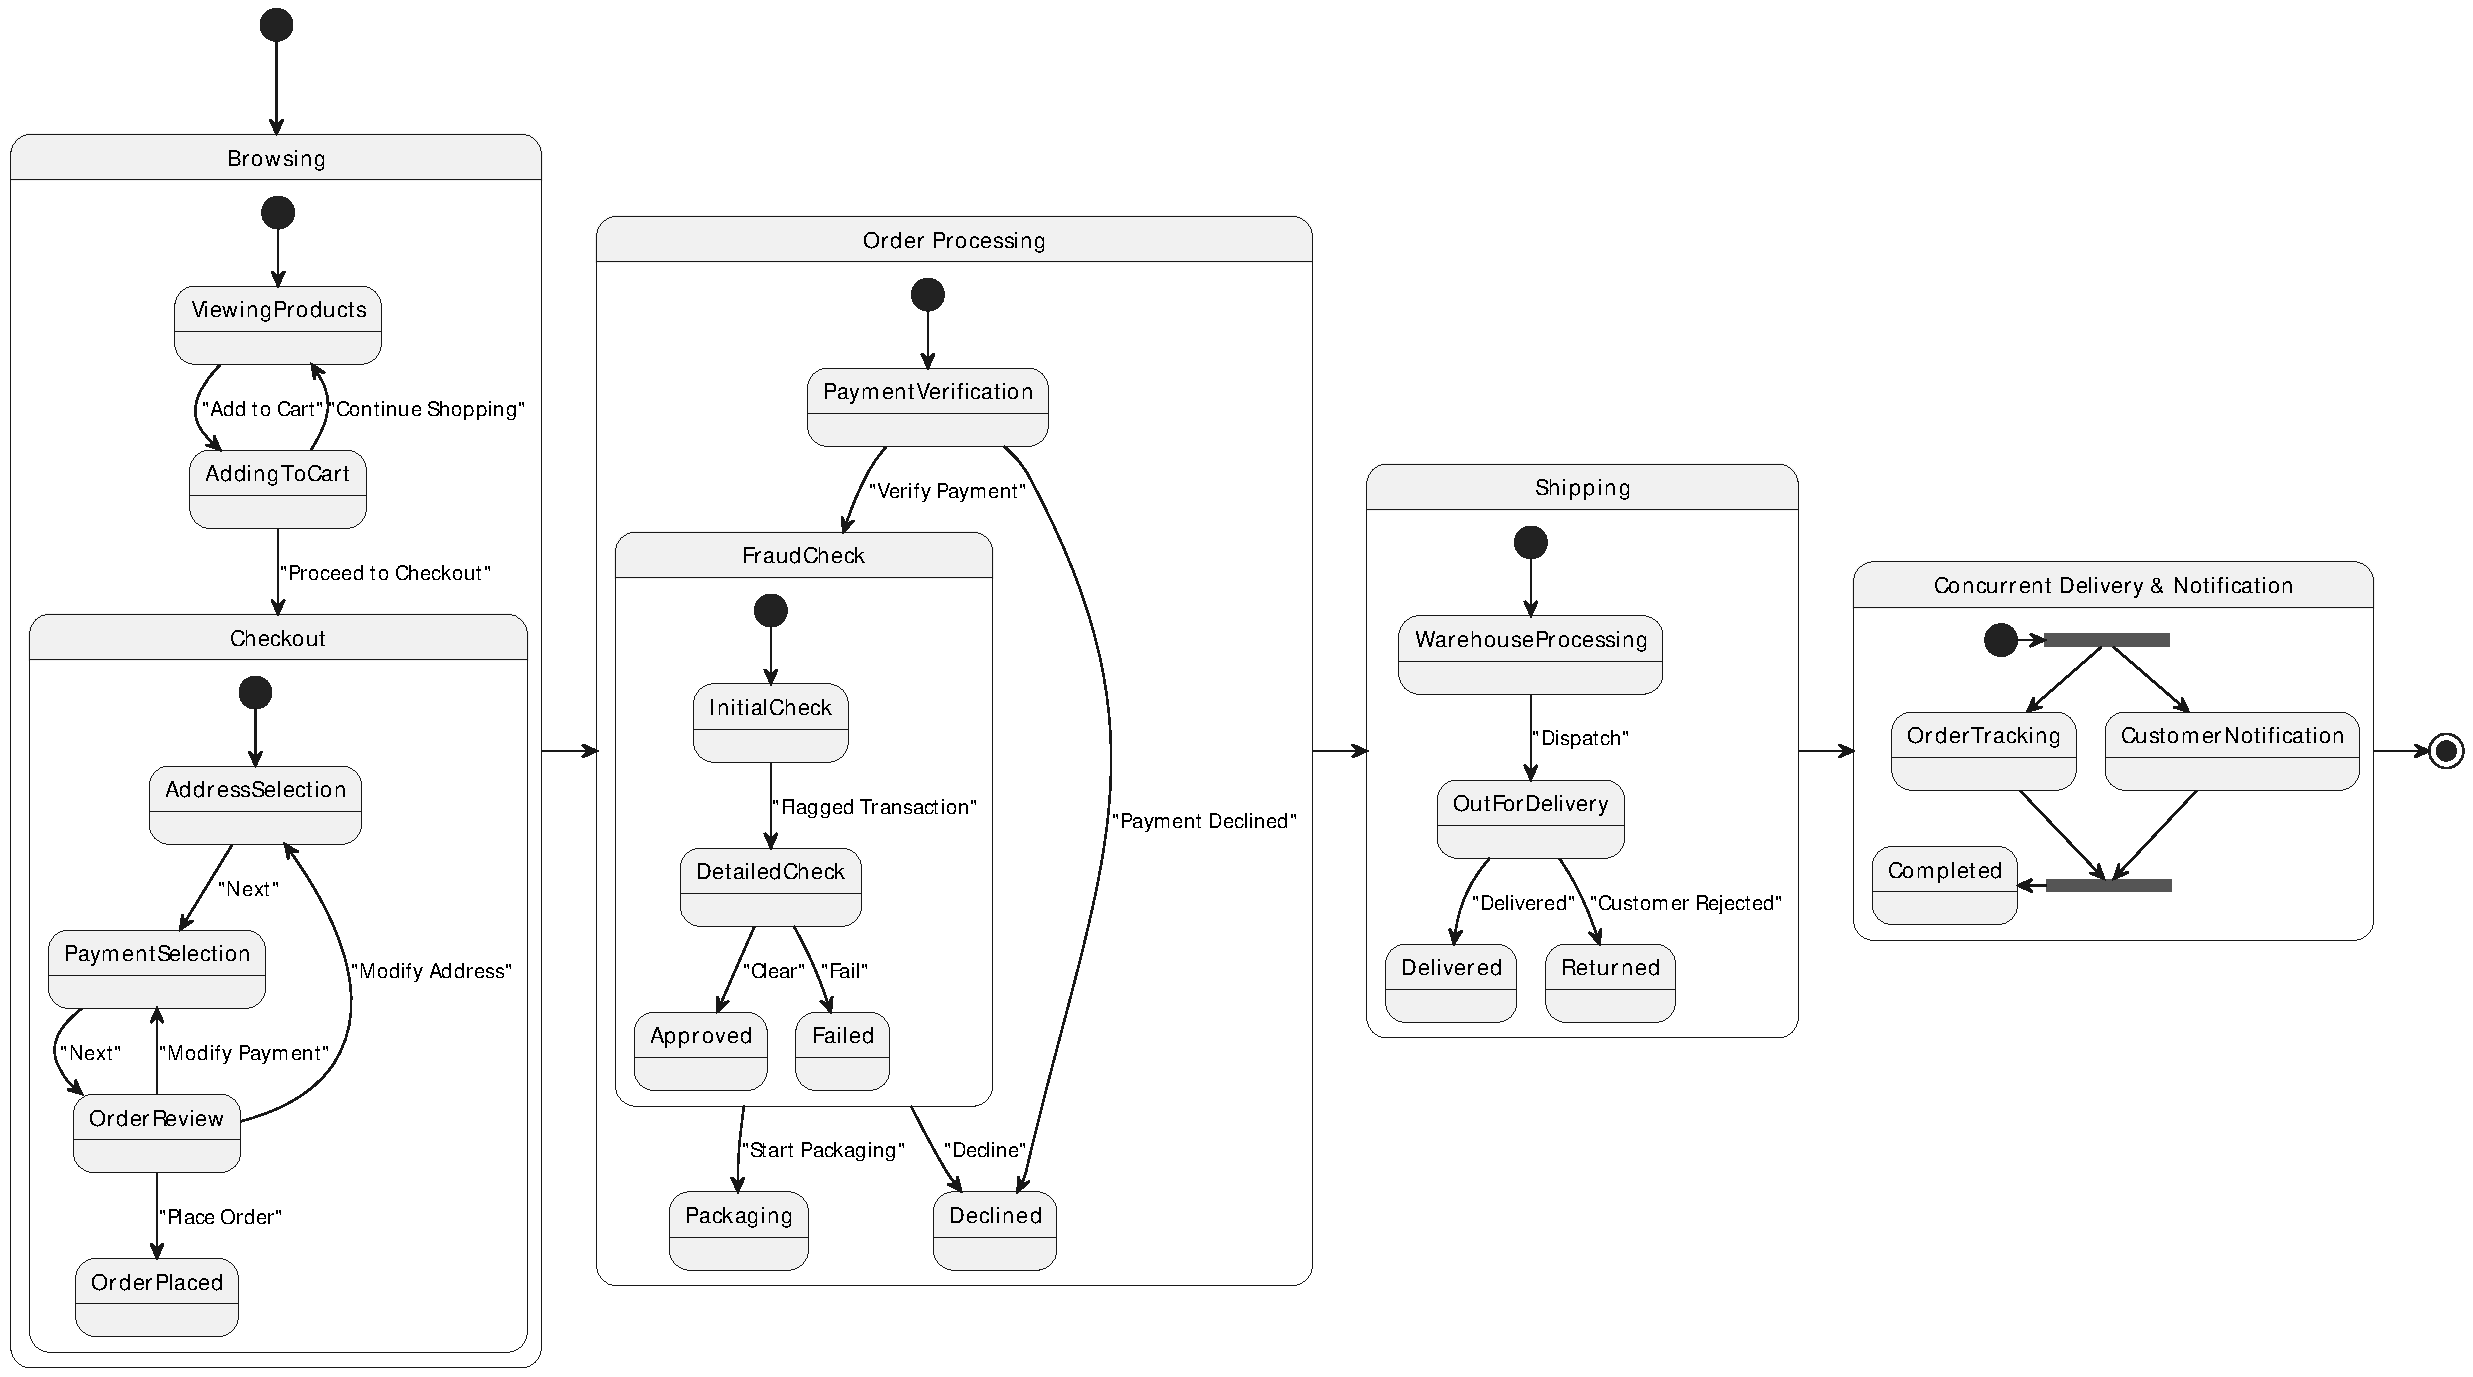
\includegraphics[width=\textwidth]{../figures/out/statechart_diagram}
	\caption{Statechart diagram and its features}
	\label{fig:statechart_diagram}
\end{figure}

\begin{lstlisting}[language=puml, caption={Statechart Diagram for E-Commerce Order Processing}]
	@startuml
	
	[*] --> Browsing
	
	state Browsing {
		[*] --> ViewingProducts
		ViewingProducts --> AddingToCart : "Add to Cart"
		AddingToCart --> ViewingProducts : "Continue Shopping"
		AddingToCart --> Checkout : "Proceed to Checkout"
	}
	
	state Checkout {
		[*] --> AddressSelection
		AddressSelection --> PaymentSelection : "Next"
		PaymentSelection --> OrderReview : "Next"
		OrderReview --> OrderPlaced : "Place Order"
		OrderReview --> AddressSelection : "Modify Address"
		OrderReview --> PaymentSelection : "Modify Payment"
	}
	
	Browsing -r-> OrderProcessing
	
	state "Order Processing" as OrderProcessing {
		[*] --> PaymentVerification
		PaymentVerification --> FraudCheck : "Verify Payment"
		PaymentVerification --> Declined : "Payment Declined"
		
		state FraudCheck {
			[*] --> InitialCheck
			InitialCheck --> DetailedCheck : "Flagged Transaction"
			DetailedCheck --> Approved : "Clear"
			DetailedCheck --> Failed : "Fail"
		}
		
		FraudCheck --> Declined: "Decline"
		FraudCheck --> Packaging : "Start Packaging"
	}
	
	OrderProcessing -r-> Shipping
	
	state "Shipping" as Shipping {
		[*] --> WarehouseProcessing
		WarehouseProcessing --> OutForDelivery : "Dispatch"
		OutForDelivery --> Delivered : "Delivered"
		OutForDelivery --> Returned : "Customer Rejected"
	}
	
	Shipping -r-> DeliveryProcess
	
	state "Concurrent Delivery & Notification" as DeliveryProcess {
		
		state fork_state <<fork>>
		[*] -r-> fork_state 
		fork_state --> OrderTracking
		fork_state --> CustomerNotification
		
		state join_state <<join>>
		OrderTracking --> join_state
		CustomerNotification --> join_state
		Completed <-- join_state
		
	}
	
	DeliveryProcess -r-> [*]
	
	@enduml
\end{lstlisting}


\subsection{Keadaan dan Transisi}
Dalam statechart diagram, sistem direpresentasikan sebagai kumpulan keadaan (state) yang berubah berdasarkan transisi. Setiap keadaan merepresentasikan kondisi tertentu yang dapat ditempati oleh suatu entitas dalam sistem. Transisi antar keadaan ditentukan oleh suatu peristiwa atau aksi. 

Dalam contoh diagram ini, sistem pemesanan e-commerce dimulai dari keadaan \texttt{Browsing}, di mana pengguna dapat menjelajahi produk, menambahkan produk ke dalam keranjang, dan melanjutkan ke proses checkout. Transisi dari \texttt{Browsing} ke \texttt{Checkout} terjadi ketika pengguna memilih untuk melakukan pembelian.

\begin{lstlisting}[language=puml]
	[*] --> Browsing
	Browsing {
		[*] --> ViewingProducts
		ViewingProducts --> AddingToCart : "Add to Cart"
		AddingToCart --> ViewingProducts : "Continue Shopping"
		AddingToCart --> Checkout : "Proceed to Checkout"
	}
\end{lstlisting}

\subsection{Keadaan Tersusun (Composite State)}
Statechart diagram mendukung keadaan tersusun (composite state) yang memungkinkan representasi keadaan yang lebih kompleks. Dalam contoh ini, \texttt{Order Processing} dan \texttt{FraudCheck} adalah contoh composite state, yang masing-masing memiliki sub-state di dalamnya. Composite state memungkinkan sistem untuk menggambarkan proses yang lebih terstruktur, seperti verifikasi pembayaran sebelum pesanan dapat diproses lebih lanjut.

\begin{lstlisting}[language=puml]
	state "Order Processing" as OrderProcessing {
		[*] --> PaymentVerification
		PaymentVerification --> FraudCheck : "Verify Payment"
		
		state FraudCheck {
			[*] --> InitialCheck
			InitialCheck --> DetailedCheck : "Flagged Transaction"
			DetailedCheck --> Approved : "Clear"
			DetailedCheck --> Failed : "Fail"
		}
		
		FraudCheck --> Packaging : "Start Packaging"
	}
\end{lstlisting}

\subsection{Transisi Bersyarat dan Penanganan Kesalahan}
Statechart diagram memungkinkan penggunaan transisi bersyarat untuk menangani keputusan logis dalam suatu sistem. Dalam proses pemesanan ini, setelah pembayaran diverifikasi, sistem melakukan pemeriksaan keamanan melalui \texttt{FraudCheck}. Jika transaksi ditandai sebagai mencurigakan, sistem melakukan pemeriksaan lebih lanjut. Jika transaksi tidak valid, sistem akan menolak pembayaran dan mengembalikan pengguna ke status \texttt{Declined}. Sebaliknya, jika transaksi valid, sistem akan melanjutkan ke proses pengemasan.

\begin{lstlisting}[language=puml]
	PaymentVerification --> FraudCheck : "Verify Payment"
	FraudCheck --> Declined : "Decline"
	FraudCheck --> Packaging : "Start Packaging"
\end{lstlisting}

\subsection{Fork dan Join untuk Eksekusi Paralel}
Dalam beberapa proses, terdapat aktivitas yang dapat berjalan secara paralel. Statechart diagram memungkinkan penggunaan \texttt{fork} dan \texttt{join} untuk merepresentasikan eksekusi bersamaan. Dalam contoh ini, setelah pesanan dikirim, sistem menjalankan dua proses paralel, yaitu pelacakan pesanan (\texttt{OrderTracking}) dan pemberitahuan pelanggan (\texttt{CustomerNotification}). Kedua proses ini berjalan secara independen dan akan digabung kembali dalam \texttt{join\_state} sebelum sistem menyelesaikan proses pengiriman.

\begin{lstlisting}[language=puml]
	state "Concurrent Delivery & Notification" as DeliveryProcess {
		
		state fork_state <<fork>>
		[*] -r-> fork_state 
		fork_state --> OrderTracking
		fork_state --> CustomerNotification
		
		state join_state <<join>>
		OrderTracking --> join_state
		CustomerNotification --> join_state
		Completed <-- join_state
	}
\end{lstlisting}

\subsection{Keadaan Awal dan Akhir}
Statechart diagram memiliki simbol keadaan awal dan akhir yang ditandai dengan \texttt{[*]}. Keadaan awal menunjukkan titik masuk sistem, sedangkan keadaan akhir menunjukkan titik keluarnya sistem. Dalam contoh diagram ini, keadaan awal dimulai dari \texttt{Browsing}, dan sistem berakhir setelah pesanan selesai diproses di keadaan \texttt{Completed}.

\begin{lstlisting}[language=puml]
	[*] --> Browsing
	Completed --> [*]
\end{lstlisting}

Statechart diagram sangat berguna untuk merepresentasikan perubahan keadaan dalam sistem yang memiliki alur kerja kompleks, seperti proses pemesanan dalam e-commerce. Dengan menggunakan elemen-elemen seperti \textbf{keadaan tersusun (composite state)}, \textbf{transisi bersyarat}, \textbf{fork dan join untuk eksekusi paralel}, serta \textbf{eadaan awal dan akhir}, diagram ini memberikan gambaran yang jelas mengenai bagaimana suatu sistem merespons berbagai kejadian selama siklus hidupnya. Dengan pemodelan ini, pengembang dapat lebih mudah memahami bagaimana sistem bekerja, mendeteksi potensi masalah, dan mengoptimalkan proses bisnis sebelum implementasi dilakukan.


\section{Use Case Diagram}

Use case diagram merupakan salah satu diagram perilaku dalam Unified Modeling Language (UML) yang digunakan untuk merepresentasikan interaksi antara pengguna (aktor) dan sistem. Diagram ini menunjukkan berbagai fungsi yang tersedia dalam sistem dan bagaimana aktor berinteraksi dengan masing-masing fungsi tersebut. 

Pada contoh ini, digunakan use case diagram untuk menggambarkan proses utama dalam sistem e-commerce, mencakup aktivitas pelanggan dalam mencari produk, menambahkan ke keranjang, melakukan checkout, hingga pelacakan pesanan. Selain itu, diagram ini juga mencakup peran admin dalam mengelola pesanan, menghasilkan laporan, serta peran sistem eksternal seperti gateway pembayaran.

\begin{figure}
	\centering
	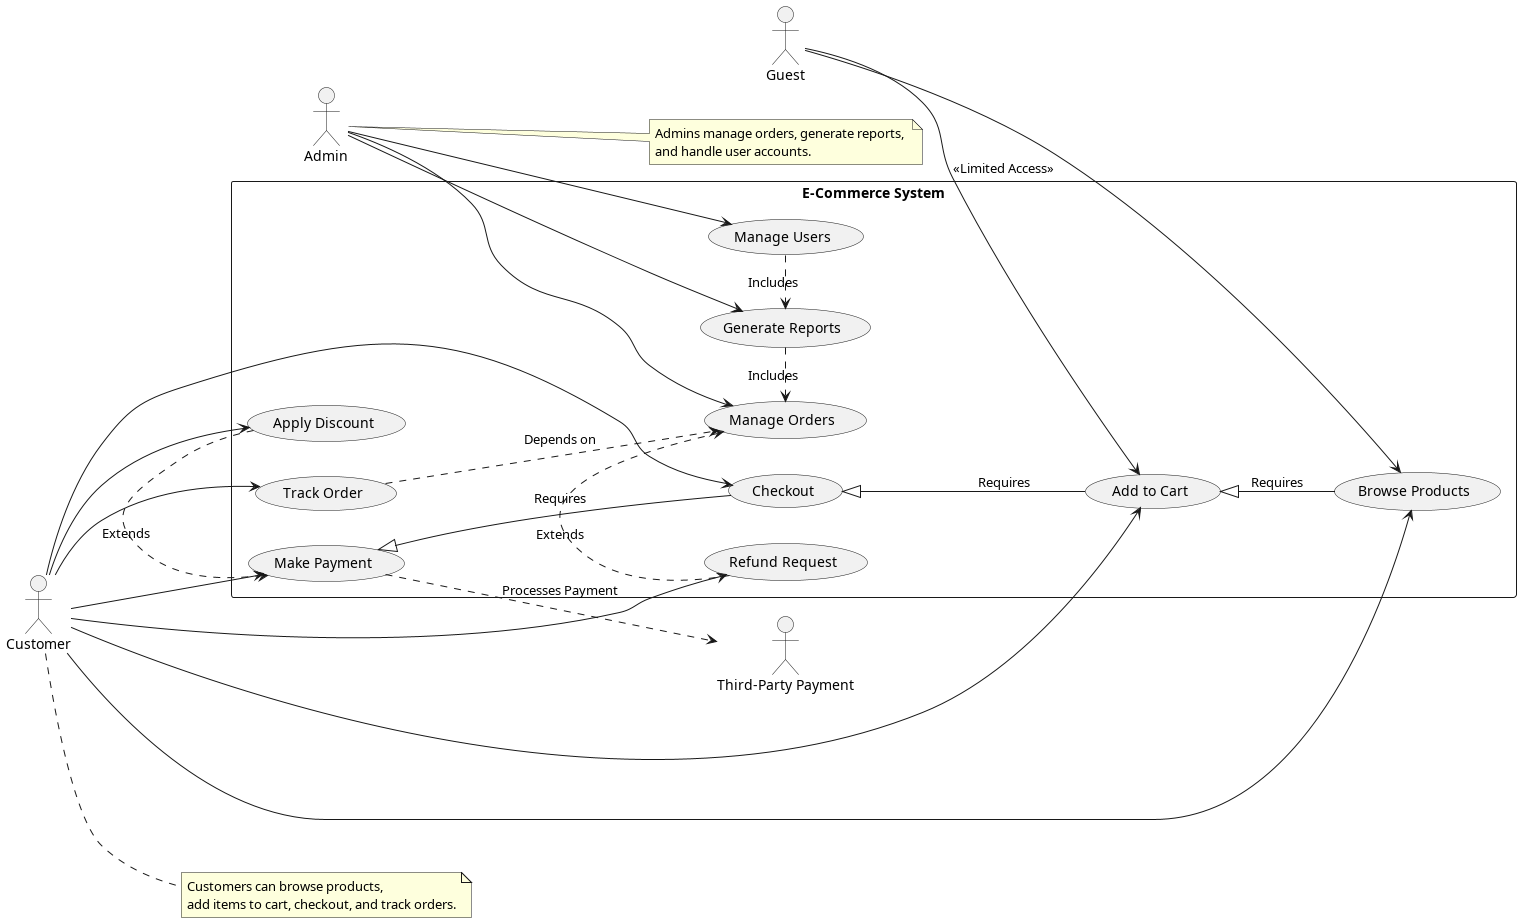
\includegraphics[width=\textwidth]{../figures/out/usecase_diagram}
	\caption{Use Case Diagram for E-Commerce System}
	\label{fig:usecase_diagram}
\end{figure}

\begin{lstlisting}[language=puml, caption={Use Case Diagram for E-Commerce System}]
	@startuml
	
	' skinparam linetype polyline
	' skinparam linetype ortho
	left to right direction
	' Define actors
	actor Customer
	actor Guest
	actor Admin
	actor "Third-Party Payment" as PaymentGateway
	
	' Define system boundary
	rectangle "E-Commerce System" {
		
		' Primary use cases
		usecase "Browse Products" as UC1
		usecase "Add to Cart" as UC2
		usecase "Checkout" as UC3
		usecase "Make Payment" as UC4
		usecase "Track Order" as UC5
		usecase "Manage Orders" as UC6
		usecase "Refund Request" as UC7
		usecase "Apply Discount" as UC8
		usecase "Generate Reports" as UC9
		usecase "Manage Users" as UC10
		
		' Relationships
		UC2 <|-- UC1 : "Requires"
		UC3 <|-- UC2 : "Requires"
		UC4 <|-- UC3 : "Requires"
		
		UC4 ..> PaymentGateway : "Processes Payment"
		UC5 ..> UC6 : "Depends on"
		UC7 .> UC6 : "Extends"
		UC8 .> UC4 : "Extends"
		
		' Admin-specific use cases
		UC9 .> UC6 : "Includes"
		UC10 .> UC9 : "Includes"
	}
	
	' Assign actors to use cases
	Customer --> UC1
	Customer --> UC2
	Customer --> UC3
	Customer --> UC4
	Customer --> UC5
	Customer --> UC7
	Customer --> UC8
	
	Guest --> UC1
	Guest --> UC2 : "<<Limited Access>>"
	
	Admin --> UC6
	Admin --> UC9
	Admin --> UC10
	
	' Notes
	note right of Customer
	Customers can browse products,
	add items to cart, checkout, and track orders.
	end note
	
	note right of Admin
	Admins manage orders, generate reports, 
	and handle user accounts.
	end note
	
	@enduml
\end{lstlisting}


\subsection{Aktor dalam Use Case Diagram}
Aktor merupakan entitas eksternal yang berinteraksi dengan sistem untuk mencapai tujuan tertentu. Dalam contoh ini, terdapat empat aktor utama:
\begin{enumerate}
	\item \textbf{Customer}, yaitu pengguna utama yang melakukan pembelian produk.
	\item \textbf{Guest}, yaitu pengguna yang dapat menjelajahi produk tetapi memiliki akses terbatas.
	\item \textbf{Admin}, yang bertanggung jawab untuk mengelola pesanan, pelanggan, dan laporan.
	\item \textbf{Third-Party Payment}, yaitu sistem eksternal yang menangani transaksi pembayaran.
\end{enumerate}

Aktor-aktor ini direpresentasikan dengan simbol stick figure dan memiliki garis koneksi ke berbagai use case dalam sistem.

\begin{lstlisting}[language=puml]
	actor Customer
	actor Guest
	actor Admin
	actor "Third-Party Payment" as PaymentGateway
\end{lstlisting}

\subsection{Use Case dan Relasi}
Use case merepresentasikan fungsi atau layanan yang tersedia dalam sistem. Dalam sistem e-commerce ini, beberapa use case utama yang tersedia meliputi:
\begin{enumerate}
	\item \textbf{Browse Products}: Pelanggan atau tamu dapat melihat daftar produk yang tersedia.
	\item \textbf{Add to Cart}: Pelanggan dapat menambahkan produk ke keranjang belanja.
	\item \textbf{Checkout}: Pelanggan melakukan proses pembayaran.
	\item \textbf{Make Payment}: Transaksi pembayaran diproses melalui gateway pembayaran eksternal.
	\item \textbf{Track Order}: Pelanggan dapat melacak status pengiriman pesanan mereka.
	\item \textbf{Manage Orders}: Admin dapat mengelola pesanan pelanggan.
	\item \textbf{Refund Request}: Pelanggan dapat mengajukan permintaan pengembalian dana jika diperlukan.
	\item \textbf{Apply Discount}: Sistem dapat menerapkan diskon saat pembayaran dilakukan.
	\item \textbf{Generate Reports}: Admin dapat menghasilkan laporan terkait transaksi dan aktivitas pengguna.
	\item \textbf{Manage Users}: Admin dapat mengelola informasi pengguna dalam sistem.
\end{enumerate}

Setiap use case direpresentasikan dengan elips dalam diagram, dan aktor yang terkait memiliki koneksi ke use case yang mereka gunakan.

\begin{lstlisting}[language=puml]
	rectangle "E-Commerce System" {
		usecase "Browse Products" as UC1
		usecase "Add to Cart" as UC2
		usecase "Checkout" as UC3
		usecase "Make Payment" as UC4
		usecase "Track Order" as UC5
		usecase "Manage Orders" as UC6
		usecase "Refund Request" as UC7
		usecase "Apply Discount" as UC8
		usecase "Generate Reports" as UC9
		usecase "Manage Users" as UC10
	}
\end{lstlisting}

\subsection{Relasi dalam Use Case Diagram}
Dalam use case diagram, terdapat beberapa jenis hubungan yang menghubungkan use case satu dengan lainnya:
\begin{enumerate}
	\item \textbf{Generalization (\texttt{<|--})}: Digunakan untuk menunjukkan bahwa satu use case merupakan bentuk spesifik dari use case lainnya. Contohnya, \texttt{Add to Cart} adalah bagian dari \texttt{Browse Products}, sedangkan \texttt{Checkout} bergantung pada \texttt{Add to Cart}.
	\begin{lstlisting}[language=puml]
		UC2 <|-- UC1 : "Requires"
		UC3 <|-- UC2 : "Requires"
		UC4 <|-- UC3 : "Requires"
	\end{lstlisting}
	
	\item \textbf{Include (\texttt{.>})}: Digunakan untuk menunjukkan bahwa satu use case selalu memanggil use case lainnya sebagai bagian dari prosesnya. Misalnya, \texttt{Generate Reports} mengandung bagian dari \texttt{Manage Orders} dan \texttt{Manage Users}.
	\begin{lstlisting}[language=puml]
		UC9 .> UC6 : "Includes"
		UC10 .> UC9 : "Includes"
	\end{lstlisting}
	
	\item \textbf{Extend (\texttt{..>})}: Menunjukkan bahwa use case dapat memperluas fungsi use case lain dalam kondisi tertentu. Sebagai contoh, \texttt{Refund Request} memperpanjang \texttt{Manage Orders} karena tidak semua pesanan akan mengalami pengembalian dana.
	\begin{lstlisting}[language=puml]
		UC7 ..> UC6 : "Extends"
		UC8 ..> UC4 : "Extends"
	\end{lstlisting}
\end{enumerate}

\subsection{Hubungan Aktor dengan Use Case}
Setiap aktor dalam sistem memiliki hubungan dengan satu atau lebih use case. Pelanggan memiliki akses ke hampir semua fitur utama, sementara tamu hanya memiliki akses terbatas. Admin memiliki akses ke fitur manajemen sistem.

\begin{lstlisting}[language=puml]
	Customer --> UC1
	Customer --> UC2
	Customer --> UC3
	Customer --> UC4
	Customer --> UC5
	Customer --> UC7
	Customer --> UC8
	
	Guest --> UC1
	Guest --> UC2 : "<<Limited Access>>"
	
	Admin --> UC6
	Admin --> UC9
	Admin --> UC10
\end{lstlisting}

\subsection{Pemberian Catatan pada Diagram}
PlantUML memungkinkan penambahan catatan untuk memberikan informasi tambahan dalam diagram. Dalam contoh ini, terdapat catatan yang menjelaskan peran masing-masing aktor dalam sistem.

\begin{lstlisting}[language=puml]
	note right of Customer
	Customers can browse products,
	add items to cart, checkout, and track orders.
	end note
	
	note right of Admin
	Admins manage orders, generate reports, 
	and handle user accounts.
	end note
\end{lstlisting}

Use case diagram memberikan gambaran bagaimana aktor berinteraksi dengan sistem melalui berbagai fungsi yang tersedia. Dalam contoh ini, sistem e-commerce memiliki berbagai aktor seperti pelanggan, tamu, admin, dan sistem pembayaran eksternal yang berinteraksi dengan beberapa use case. Dengan menggunakan hubungan seperti \textbf{generalization, include, dan extend}, diagram ini memberikan representasi yang jelas mengenai bagaimana fitur dalam sistem saling berkaitan.

Use case diagram sangat berguna dalam tahap perancangan perangkat lunak karena dapat membantu pemangku kepentingan dalam memahami bagaimana pengguna berinteraksi dengan sistem sebelum implementasi dilakukan.

\section{Referensi}
Untuk pembelajaran lebih mendalam mengenai UML, silahkan kunjungi tautan berikut: \url{https://www.uml-diagrams.org/}.

	\chapter{Prinsip Desain Berorientasi Objek (SOLID)}

\section{Pendahuluan}

Desain perangkat lunak berorientasi objek yang baik tidak hanya ditentukan oleh kemampuan untuk menyelesaikan masalah, tetapi juga oleh kemampuannya dalam menangani perubahan, mempertahankan kualitas kode, dan memudahkan kolaborasi tim pengembang. Seiring bertambahnya kompleksitas sistem, desain yang tidak terstruktur dapat menyebabkan kode sulit dipelihara, rentan terhadap bug saat mengalami perubahan, dan sulit diuji secara terpisah.

Untuk mengatasi permasalahan tersebut, Robert C. Martin memperkenalkan lima prinsip desain berorientasi objek yang dikenal dengan akronim SOLID: \textit{Single Responsibility Principle}, \textit{Open/Closed Principle}, \textit{Liskov Substitution Principle}, \textit{Interface Segregation Principle}, dan \textit{Dependency Inversion Principle}. Prinsip-prinsip ini bertujuan untuk menghasilkan sistem yang modular, fleksibel terhadap perubahan, dan memiliki dependensi yang minimal antar komponen.

Masing-masing prinsip memiliki fokus yang spesifik. SRP menekankan pentingnya memisahkan tanggung jawab dalam kelas, OCP mendorong ekstensi tanpa modifikasi, LSP memastikan substitusi subclass tanpa melanggar kontrak perilaku, ISP menghindari antarmuka gemuk yang membebani klien, dan DIP membalik ketergantungan dari detail implementasi ke arah abstraksi. Secara keseluruhan, SOLID membantu membentuk fondasi yang kuat untuk pengembangan perangkat lunak jangka panjang.

Bab ini akan membahas kelima prinsip SOLID secara terstruktur, dimulai dari pengertian dasar, manfaat dan kekurangannya, serta contoh implementasi dan pelanggarannya dalam praktik. Pemahaman terhadap prinsip-prinsip ini tidak hanya membantu menghasilkan desain yang elegan, tetapi juga meningkatkan kualitas perangkat lunak dari segi keterkelolaan, skalabilitas, pengujian, serta efisiensi sumber daya dalam jangka panjang.


\section{Single Responsibility Principle (SRP)}

\subsection{Pengertian dan Konsep Dasar}
Single Responsibility Principle (SRP) menyatakan bahwa sebuah kelas sebaiknya hanya memiliki satu alasan untuk berubah, yaitu hanya menangani satu tanggung jawab utama. Prinsip ini bertujuan untuk memisahkan fungsionalitas yang berbeda ke dalam kelas-kelas yang berbeda, sehingga setiap kelas hanya fokus pada satu aspek dari sistem. Dengan mengikuti SRP, struktur kode menjadi lebih modular, mudah dipahami, dan lebih mudah diuji secara unit.

\subsection{Manfaat dan Kekurangan}
Manfaat utama dari penerapan SRP adalah peningkatan keterbacaan dan pemeliharaan kode. Perubahan dalam satu tanggung jawab tidak akan berdampak pada bagian kode lain yang tidak terkait. Selain itu, pengujian unit dapat dilakukan lebih spesifik karena setiap kelas memiliki satu peran jelas. Namun, kekurangannya adalah potensi bertambahnya jumlah kelas dalam proyek, yang dapat meningkatkan kompleksitas manajemen struktur proyek.

\subsection{Contoh Kasus 1}
Salah satu contoh pelanggaran prinsip ini adalah ketika sebuah kelas tidak hanya bertanggung jawab untuk mengelola data tetapi juga menangani logika bisnis dan penyimpanan ke basis data. Sebagai contoh, sebuah kelas \texttt{Invoice} yang bertanggung jawab menghitung total belanja, mencetak faktur, dan menyimpan data ke file. Kelas ini memiliki lebih dari satu alasan untuk berubah: perubahan pada logika bisnis, format cetak, dan format penyimpanan akan mempengaruhi kelas yang sama.

\begin{lstlisting}[style=JavaStyle, caption={Contoh pelanggaran SRP}]
	public class Invoice {
		private List<Item> items;
		
		public double calculateTotal() {
			// Hitung total harga
		}
		
		public void printInvoice() {
			// Cetak faktur ke printer
		}
		
		public void saveToFile() {
			// Simpan data faktur ke file
		}
	}
\end{lstlisting}

\begin{lstlisting}[style=JavaStyle, caption={Refaktor menggunakan SRP}]
	public class Invoice {
		private List<Item> items;
		
		public double calculateTotal() {
			// Hitung total harga
		}
	}
	
	public class InvoicePrinter {
		public void print(Invoice invoice) {
			// Cetak faktur ke printer
		}
	}
	
	public class InvoiceSaver {
		public void saveToFile(Invoice invoice) {
			// Simpan data faktur ke file
		}
	}
\end{lstlisting}

Dengan memisahkan tanggung jawab ke dalam kelas-kelas khusus seperti \texttt{InvoicePrinter} dan \texttt{InvoiceSaver}, kode menjadi lebih terorganisir dan sesuai dengan prinsip SRP.

\subsection{Contoh Kasus 2}
Contoh lain dari pelanggaran SRP adalah pada kelas \texttt{User}. Dalam beberapa implementasi, kelas ini tidak hanya menyimpan data pengguna, tetapi juga menangani validasi data dan pengiriman email. Ketiga tanggung jawab tersebut seharusnya dipisahkan agar perubahan pada satu aspek (misalnya format email) tidak memengaruhi logika validasi atau struktur data pengguna.

\begin{lstlisting}[style=JavaStyle, caption={Contoh pelanggaran SRP}]
	public class User {
		private String name;
		private String email;
		
		public boolean isValidEmail() {
			// Validasi format email
		}
		
		public void sendWelcomeEmail() {
			// Kirim email sambutan
		}
	}
\end{lstlisting}

\begin{lstlisting}[style=JavaStyle, caption={Refaktor menggunakan SRP}]
	public class User {
		private String name;
		private String email;
		
		public String getEmail() {
			return email;
		}
	}
	
	public class EmailValidator {
		public boolean isValid(String email) {
			// Validasi format email
		}
	}
	
	public class EmailSender {
		public void sendWelcomeEmail(String email) {
			// Kirim email sambutan
		}
	}
\end{lstlisting}

Dengan memisahkan validasi dan pengiriman email ke dalam kelas \texttt{EmailValidator} dan \texttt{EmailSender}, maka setiap kelas memiliki satu tanggung jawab yang jelas. Hal ini membuat kode lebih modular, mudah diuji, dan tidak rentan terhadap perubahan yang tidak terkait langsung.

\section{Open/Closed Principle (OCP)}

\subsection{Pengertian dan Konsep Dasar}
Open/Closed Principle (OCP) menyatakan bahwa entitas perangkat lunak seperti kelas, modul, atau fungsi harus terbuka untuk ekstensi tetapi tertutup untuk modifikasi. Prinsip ini pertama kali diperkenalkan oleh Bertrand Meyer dan kemudian menjadi bagian penting dalam prinsip SOLID. "Terbuka untuk ekstensi" berarti bahwa perilaku suatu entitas dapat ditingkatkan atau diperluas tanpa harus mengubah struktur atau kode yang sudah ada. "Tertutup untuk modifikasi" berarti bahwa kode sumber asli tidak perlu diubah untuk memenuhi kebutuhan baru.

Penerapan OCP sangat erat kaitannya dengan penggunaan abstraksi, seperti antarmuka dan kelas abstrak, serta pola desain seperti *Strategy*, *Decorator*, dan *Factory Method*. Dengan menggunakan mekanisme tersebut, pengembang dapat menambahkan fungsionalitas baru dengan cara mewarisi atau mengimplementasikan abstraksi yang sudah ada tanpa menyentuh kode lama.

\subsection{Manfaat dan Kekurangan}
Penerapan Open/Closed Principle memberikan sejumlah manfaat signifikan. Pertama, prinsip ini meningkatkan stabilitas sistem karena perubahan kebutuhan baru tidak memerlukan perubahan terhadap bagian sistem yang sudah berjalan dengan baik. Kedua, kode menjadi lebih fleksibel dan mudah dikembangkan karena fungsionalitas dapat ditambahkan melalui ekstensi. Selain itu, OCP mendukung reuse dan modularitas dengan memisahkan perilaku ke dalam komponen-komponen yang dapat dikembangkan secara independen.

Namun, kekurangan dari prinsip ini adalah adanya kompleksitas tambahan yang muncul akibat penggunaan abstraksi yang berlebihan. Dalam beberapa kasus, penerapan OCP dapat menghasilkan struktur kode yang terlalu banyak kelas atau antarmuka, terutama bila digunakan secara berlebihan pada sistem yang belum memerlukan fleksibilitas tinggi. Oleh karena itu, penerapan prinsip ini perlu dilakukan secara bertahap dan berdasarkan kebutuhan sistem yang berkembang.

\subsection{Contoh Kasus 1}
Sebuah contoh pelanggaran prinsip Open/Closed terjadi ketika logika program harus dimodifikasi setiap kali ada jenis baru dari sebuah entitas. Misalnya, pada sistem pembayaran, terdapat kelas \texttt{PaymentProcessor} yang menangani berbagai metode pembayaran seperti \texttt{CreditCard} dan \texttt{BankTransfer}. Jika ditambahkan metode baru seperti \texttt{EWallet}, maka kode di dalam \texttt{PaymentProcessor} harus diubah. Hal ini menunjukkan bahwa kelas tidak tertutup untuk modifikasi dan tidak mengikuti prinsip OCP.

\begin{lstlisting}[style=JavaStyle, caption={Contoh pelanggaran OCP}]
	public class PaymentProcessor {
		public void process(String paymentType) {
			if (paymentType.equals("CreditCard")) {
				// Proses pembayaran dengan kartu kredit
			} else if (paymentType.equals("BankTransfer")) {
				// Proses pembayaran dengan transfer bank
			}
		}
	}
\end{lstlisting}

Jika sistem diperluas untuk mendukung metode baru seperti \texttt{EWallet}, maka kode \texttt{PaymentProcessor} harus dimodifikasi, yang bertentangan dengan prinsip OCP.

Refaktorisasi dapat dilakukan dengan menggunakan abstraksi berupa antarmuka \texttt{PaymentMethod}. Dengan pendekatan ini, kelas \texttt{PaymentProcessor} tidak perlu diubah ketika metode pembayaran baru ditambahkan.

\begin{lstlisting}[style=JavaStyle, caption={Refaktor menggunakan OCP}]
	public interface PaymentMethod {
		void process();
	}
	
	public class CreditCardPayment implements PaymentMethod {
		public void process() {
			// Proses pembayaran dengan kartu kredit
		}
	}
	
	public class BankTransferPayment implements PaymentMethod {
		public void process() {
			// Proses pembayaran dengan transfer bank
		}
	}
	
	public class PaymentProcessor {
		public void process(PaymentMethod method) {
			method.process();
		}
	}
\end{lstlisting}

Dengan pendekatan ini, penambahan metode baru seperti \texttt{EWalletPayment} cukup dilakukan dengan membuat kelas baru yang mengimplementasikan antarmuka \texttt{PaymentMethod}, tanpa perlu menyentuh kelas \texttt{PaymentProcessor}. Hal ini menunjukkan penerapan prinsip Open/Closed dengan baik.

\subsection{Contoh Kasus 2}
Contoh pelanggaran prinsip Open/Closed juga dapat ditemukan pada sistem notifikasi. Misalnya, sebuah kelas \texttt{NotificationService} mengirimkan pesan kepada pengguna melalui beberapa saluran seperti email dan SMS. Jika suatu saat dibutuhkan saluran baru seperti \texttt{PushNotification}, maka kode pada \texttt{NotificationService} harus dimodifikasi. Ini berarti kelas tidak tertutup untuk modifikasi dan melanggar prinsip OCP.

\begin{lstlisting}[style=JavaStyle, caption={Contoh pelanggaran OCP}]
	public class NotificationService {
		public void send(String channel, String message) {
			if (channel.equals("email")) {
				// Kirim email
			} else if (channel.equals("sms")) {
				// Kirim SMS
			}
		}
	}
\end{lstlisting}

Untuk menambahkan saluran baru, seperti notifikasi melalui aplikasi, pengembang harus menambahkan blok kode baru dalam metode \texttt{send}, sehingga kode lama harus diubah.

Refaktorisasi dapat dilakukan dengan membuat antarmuka \texttt{Notifier} dan mengimplementasikannya untuk setiap jenis saluran. Dengan pendekatan ini, \texttt{NotificationService} cukup memanggil metode \texttt{send} dari objek yang sesuai, tanpa mengetahui detail dari saluran yang digunakan.

\begin{lstlisting}[style=JavaStyle, caption={Refaktor menggunakan OCP}]
	public interface Notifier {
		void send(String message);
	}
	
	public class EmailNotifier implements Notifier {
		public void send(String message) {
			// Kirim email
		}
	}
	
	public class SMSNotifier implements Notifier {
		public void send(String message) {
			// Kirim SMS
		}
	}
	
	public class NotificationService {
		public void sendNotification(Notifier notifier, String message) {
			notifier.send(message);
		}
	}
\end{lstlisting}

Dengan struktur ini, penambahan jenis notifikasi baru cukup dilakukan dengan membuat kelas baru seperti \texttt{PushNotifier} yang mengimplementasikan \texttt{Notifier}, tanpa perlu mengubah kode pada \texttt{NotificationService}. Ini menunjukkan bahwa sistem telah dirancang sesuai dengan prinsip Open/Closed.


\section{Liskov Substitution Principle (LSP)}

\subsection{Pengertian dan Konsep Dasar}
Liskov Substitution Principle (LSP) adalah prinsip ketiga dari SOLID yang diperkenalkan oleh Barbara Liskov pada tahun 1987. Prinsip ini menyatakan bahwa objek dari subclass harus dapat menggantikan objek dari superclass tanpa mengubah kebenaran atau perilaku yang diharapkan dari program. Dalam konteks pemrograman berorientasi objek, ini berarti bahwa subclass harus mempertahankan kontrak yang ditetapkan oleh superclass, baik dari segi antarmuka maupun perilaku.

Inti dari LSP adalah memastikan bahwa pewarisan tidak merusak fungsi program. Meskipun secara sintaksis subclass dapat digunakan di tempat superclass, tetapi jika perilaku yang dihasilkan tidak sesuai dengan harapan, maka pewarisan tersebut dianggap melanggar prinsip ini. LSP mendorong desain kelas yang bersifat substitutable secara logis, bukan hanya struktural.

\subsection{Manfaat dan Kekurangan}
Penerapan Liskov Substitution Principle membawa sejumlah manfaat penting. Pertama, prinsip ini meningkatkan keandalan sistem melalui jaminan bahwa substitusi antar kelas tidak akan menyebabkan perilaku yang tidak diinginkan. Hal ini mendukung pewarisan yang aman dan mendorong penggunaan polimorfisme secara efektif. Kedua, prinsip ini memperkuat kontrak antarkelas, sehingga dokumentasi, pengujian, dan pemeliharaan kode menjadi lebih konsisten dan dapat diprediksi.

Namun, tantangan dalam menerapkan LSP adalah kebutuhan untuk menjaga kesesuaian perilaku antara superclass dan subclass, yang seringkali tidak hanya bersifat teknis tetapi juga konseptual. Jika subclass memperkenalkan perilaku yang menyimpang, maka ia bisa merusak sistem secara diam-diam. Selain itu, dalam upaya memaksakan substitusi, pengembang dapat terjebak dalam desain yang terlalu umum atau tidak realistis, terutama jika abstraksi awal tidak dirancang dengan matang.

\subsection{Contoh Kasus 1}
Salah satu contoh klasik dari pelanggaran prinsip Liskov Substitution adalah dalam pewarisan antara \texttt{Rectangle} dan \texttt{Square}. Secara logika, persegi (\texttt{Square}) adalah bentuk khusus dari persegi panjang (\texttt{Rectangle}), tetapi dari sudut pandang perilaku kelas, pewarisan ini dapat menyebabkan pelanggaran LSP.

Jika kelas \texttt{Square} mewarisi dari \texttt{Rectangle} dan mengubah perilaku metode \texttt{setWidth} atau \texttt{setHeight}, maka objek \texttt{Square} tidak lagi bisa menggantikan objek \texttt{Rectangle} tanpa memengaruhi hasil program.

\begin{lstlisting}[style=JavaStyle, caption={Contoh pelanggaran LSP}]
	public class Rectangle {
		protected int width;
		protected int height;
		
		public void setWidth(int width) {
			this.width = width;
		}
		
		public void setHeight(int height) {
			this.height = height;
		}
		
		public int getArea() {
			return width * height;
		}
	}
	
	public class Square extends Rectangle {
		@Override
		public void setWidth(int width) {
			this.width = width;
			this.height = width;
		}
		
		@Override
		public void setHeight(int height) {
			this.width = height;
			this.height = height;
		}
	}
\end{lstlisting}

Jika sebuah fungsi mengharapkan objek \texttt{Rectangle} dan mengubah lebar dan tinggi secara terpisah, maka perilaku objek \texttt{Square} akan menyimpang dari yang diharapkan, sehingga terjadi pelanggaran terhadap prinsip LSP.

\begin{lstlisting}[style=JavaStyle, caption={Fungsi yang melanggar substitusi LSP}]
	public void resizeRectangle(Rectangle r) {
		r.setWidth(5);
		r.setHeight(10);
		System.out.println("Expected area: 50, Actual area: " + r.getArea());
	}
\end{lstlisting}

Jika objek \texttt{Square} digunakan sebagai parameter fungsi tersebut, maka hasil area tidak akan sesuai dengan ekspektasi.

Solusi untuk masalah ini adalah dengan tidak menggunakan pewarisan langsung antara \texttt{Square} dan \texttt{Rectangle}, melainkan memisahkan keduanya dan mengandalkan abstraksi seperti antarmuka atau kelas dasar yang lebih umum.

\begin{lstlisting}[style=JavaStyle, caption={Refaktor: hindari pewarisan langsung}]
	public interface Shape {
		int getArea();
	}
	
	public class Rectangle implements Shape {
		private int width;
		private int height;
		
		public Rectangle(int width, int height) {
			this.width = width;
			this.height = height;
		}
		
		public int getArea() {
			return width * height;
		}
	}
	
	public class Square implements Shape {
		private int side;
		
		public Square(int side) {
			this.side = side;
		}
		
		public int getArea() {
			return side * side;
		}
	}
\end{lstlisting}

Dengan pemisahan ini, substitusi dapat dilakukan melalui antarmuka \texttt{Shape}, dan perilaku masing-masing bentuk tetap sesuai dengan ekspektasi, sehingga prinsip LSP dipenuhi.


\subsection{Contoh Kasus 2}
Contoh pelanggaran LSP juga dapat terjadi dalam desain sistem akun bank. Misalnya, kita memiliki kelas \texttt{BankAccount} yang mendukung operasi penarikan dana, dan kemudian kita membuat subclass \texttt{FixedDepositAccount} yang tidak mengizinkan penarikan dana sebelum jatuh tempo. Jika \texttt{FixedDepositAccount} mewarisi \texttt{BankAccount} tetapi perilaku \texttt{withdraw} berbeda atau menimbulkan error, maka substitusi objek tidak dapat dilakukan tanpa efek samping.

\begin{lstlisting}[style=JavaStyle, caption={Contoh pelanggaran LSP}]
	public class BankAccount {
		protected double balance;
		
		public void deposit(double amount) {
			balance += amount;
		}
		
		public void withdraw(double amount) {
			balance -= amount;
		}
		
		public double getBalance() {
			return balance;
		}
	}
	
	public class FixedDepositAccount extends BankAccount {
		@Override
		public void withdraw(double amount) {
			throw new UnsupportedOperationException("Withdrawals not allowed before maturity");
		}
	}
\end{lstlisting}

Jika program menerima objek \texttt{BankAccount} dan mencoba melakukan penarikan, maka objek \texttt{FixedDepositAccount} tidak dapat disubstitusikan tanpa menyebabkan perilaku tak terduga (dalam hal ini, pengecualian).

\begin{lstlisting}[style=JavaStyle, caption={Pemanggilan yang melanggar LSP}]
	public void processWithdrawal(BankAccount account, double amount) {
		account.withdraw(amount); // Dapat menyebabkan error jika objek adalah FixedDepositAccount
	}
\end{lstlisting}

Untuk memperbaiki pelanggaran ini, kita dapat mendesain ulang hierarki dengan membuat antarmuka yang lebih spesifik, lalu hanya mengizinkan akun-akun yang mendukung penarikan untuk mengimplementasikannya.

\begin{lstlisting}[style=JavaStyle, caption={Refaktor: gunakan abstraksi yang tepat}]
	public interface WithdrawableAccount {
		void withdraw(double amount);
		double getBalance();
	}
	
	public class SavingsAccount implements WithdrawableAccount {
		private double balance;
		
		public void deposit(double amount) {
			balance += amount;
		}
		
		public void withdraw(double amount) {
			balance -= amount;
		}
		
		public double getBalance() {
			return balance;
		}
	}
	
	public class FixedDepositAccount {
		private double balance;
		
		public void deposit(double amount) {
			balance += amount;
		}
		
		public double getBalance() {
			return balance;
		}
		
		// Tidak memiliki metode withdraw
	}
\end{lstlisting}

Dengan pendekatan ini, hanya akun yang benar-benar mendukung penarikan yang akan mengimplementasikan \texttt{WithdrawableAccount}, sehingga prinsip LSP tetap terjaga. Penggunaan antarmuka memisahkan perilaku dan memastikan substitusi yang aman sesuai kontrak perilaku.


\section{Interface Segregation Principle (ISP)}

\subsection{Pengertian dan Konsep Dasar}
Interface Segregation Principle (ISP) adalah prinsip keempat dalam SOLID yang menyatakan bahwa sebuah antarmuka sebaiknya tidak memaksakan klien untuk bergantung pada metode-metode yang tidak mereka gunakan. Prinsip ini menekankan bahwa antarmuka yang besar dan serbaguna perlu dipecah menjadi antarmuka-antarmuka yang lebih kecil dan spesifik sesuai kebutuhan klien.

ISP mendorong desain yang lebih modular dan fleksibel dengan meminimalkan ketergantungan yang tidak diperlukan. Ketika suatu antarmuka memiliki terlalu banyak metode, kelas yang mengimplementasikannya berisiko terpaksa menyediakan implementasi yang tidak relevan atau bahkan kosong, yang bertentangan dengan prinsip tanggung jawab tunggal dan prinsip substitusi.

Prinsip ini biasanya diterapkan dengan cara memecah antarmuka besar menjadi beberapa antarmuka kecil yang masing-masing mendefinisikan perilaku spesifik. Klien hanya perlu mengetahui dan bergantung pada antarmuka yang benar-benar mereka butuhkan.

\subsection{Manfaat dan Kekurangan}
Penerapan Interface Segregation Principle membawa beberapa manfaat penting. Pertama, ia meningkatkan keterpisahan kekhawatiran (\textit{separation of concerns}) karena kelas hanya bergantung pada antarmuka yang relevan dengan perannya. Kedua, hal ini mengurangi dampak perubahan—modifikasi pada satu antarmuka kecil tidak akan memengaruhi kelas-kelas lain yang tidak menggunakannya. Selain itu, ISP mendukung desain yang lebih mudah diuji karena antarmuka menjadi lebih sederhana dan terfokus.

Namun, kelemahan dari penerapan ISP dapat muncul jika pemecahan antarmuka dilakukan secara berlebihan. Hal ini dapat mengarah pada terlalu banyak antarmuka kecil yang tersebar, menyulitkan navigasi dan pemeliharaan kode. Selain itu, jika antarmuka terlalu sempit atau terlalu terfragmentasi, pengembang mungkin mengalami kesulitan dalam mengintegrasikan fungsionalitas yang seharusnya saling berkaitan.

Oleh karena itu, penerapan ISP perlu dilakukan dengan pertimbangan terhadap keseimbangan antara keterpisahan dan keterpaduan antarmuka, serta konteks penggunaan dari setiap antarmuka tersebut.

\subsection{Contoh Kasus 1}
Salah satu contoh umum pelanggaran Interface Segregation Principle terjadi ketika antarmuka didefinisikan terlalu besar dan mencakup terlalu banyak tanggung jawab. Misalnya, dalam sistem manajemen perangkat multifungsi, dibuat sebuah antarmuka \texttt{Machine} yang mencakup metode untuk mencetak, memindai, dan mengirim faks. Masalah muncul ketika perangkat tertentu, seperti printer sederhana, hanya dapat mencetak dan tidak mendukung pemindaian atau faks.

\begin{lstlisting}[style=JavaStyle, caption={Contoh pelanggaran ISP}]
	public interface Machine {
		void print(Document d);
		void scan(Document d);
		void fax(Document d);
	}
	
	public class OldPrinter implements Machine {
		public void print(Document d) {
			// Melakukan pencetakan
		}
		
		public void scan(Document d) {
			throw new UnsupportedOperationException("Scan not supported");
		}
		
		public void fax(Document d) {
			throw new UnsupportedOperationException("Fax not supported");
		}
	}
\end{lstlisting}

Kelas \texttt{OldPrinter} terpaksa mengimplementasikan metode \texttt{scan()} dan \texttt{fax()}, padahal tidak memiliki kemampuan tersebut. Ini merupakan pelanggaran terhadap ISP karena klien dipaksa bergantung pada metode yang tidak digunakan.

Untuk memperbaikinya, antarmuka \texttt{Machine} dapat dipecah menjadi beberapa antarmuka kecil yang merepresentasikan kemampuan spesifik, seperti \texttt{Printable}, \texttt{Scannable}, dan \texttt{Faxable}.

\begin{lstlisting}[style=JavaStyle, caption={Refaktor menggunakan ISP}]
	public interface Printable {
		void print(Document d);
	}
	
	public interface Scannable {
		void scan(Document d);
	}
	
	public interface Faxable {
		void fax(Document d);
	}
	
	public class OldPrinter implements Printable {
		public void print(Document d) {
			// Melakukan pencetakan
		}
	}
\end{lstlisting}

Dengan cara ini, kelas hanya bergantung pada antarmuka yang relevan. \texttt{OldPrinter} tidak lagi dipaksa untuk mengimplementasikan metode yang tidak didukung, sehingga prinsip ISP dipenuhi. Refaktorisasi ini juga membuat sistem lebih fleksibel jika di masa depan ingin menambahkan perangkat baru dengan kombinasi kapabilitas yang berbeda.

\subsection{Contoh Kasus 2}
Dalam sistem e-learning, kita bisa menemukan pelanggaran ISP ketika antarmuka \texttt{User} didefinisikan secara umum untuk mencakup semua jenis pengguna, seperti mahasiswa, dosen, dan administrator. Misalnya, antarmuka berikut memuat metode-metode untuk mengakses materi, mengajar kelas, dan mengelola sistem.

\begin{lstlisting}[style=JavaStyle, caption={Contoh pelanggaran ISP}]
	public interface User {
		void viewCourse();
		void teachCourse();
		void manageSystem();
	}
	
	public class Student implements User {
		public void viewCourse() {
			// Mahasiswa melihat materi
		}
		
		public void teachCourse() {
			throw new UnsupportedOperationException("Mahasiswa tidak mengajar");
		}
		
		public void manageSystem() {
			throw new UnsupportedOperationException("Mahasiswa tidak mengelola sistem");
		}
	}
\end{lstlisting}

Kelas \texttt{Student} terpaksa mengimplementasikan metode \texttt{teachCourse()} dan \texttt{manageSystem()}, meskipun tidak relevan dengan perannya. Ini menyebabkan ketergantungan yang tidak perlu dan melanggar prinsip ISP.

Solusi yang sesuai adalah dengan memecah antarmuka \texttt{User} menjadi beberapa antarmuka yang lebih spesifik, misalnya \texttt{CourseViewer}, \texttt{CourseInstructor}, dan \texttt{SystemManager}.

\begin{lstlisting}[style=JavaStyle, caption={Refaktor menggunakan ISP}]
	public interface CourseViewer {
		void viewCourse();
	}
	
	public interface CourseInstructor {
		void teachCourse();
	}
	
	public interface SystemManager {
		void manageSystem();
	}
	
	public class Student implements CourseViewer {
		public void viewCourse() {
			// Mahasiswa melihat materi
		}
	}
	
	public class Lecturer implements CourseViewer, CourseInstructor {
		public void viewCourse() {
			// Dosen melihat materi
		}
		
		public void teachCourse() {
			// Dosen mengajar kelas
		}
	}
	
	public class Admin implements CourseViewer, SystemManager {
		public void viewCourse() {
			// Admin melihat materi
		}
		
		public void manageSystem() {
			// Admin mengelola sistem
		}
	}
\end{lstlisting}

Dengan desain ini, setiap kelas hanya bergantung pada antarmuka yang sesuai dengan tanggung jawabnya. Prinsip ISP dipenuhi, kode menjadi lebih modular, dan setiap jenis pengguna hanya mengetahui metode yang relevan untuknya.

\section{Dependency Inversion Principle (DIP)}

\subsection{Pengertian dan Konsep Dasar}
Dependency Inversion Principle (DIP) adalah prinsip kelima dalam SOLID yang menekankan pentingnya membalik arah ketergantungan dalam desain perangkat lunak. Prinsip ini menyatakan dua hal utama:

\begin{enumerate}
	\item Modul tingkat tinggi tidak boleh bergantung pada modul tingkat rendah. Keduanya harus bergantung pada abstraksi.
	\item Abstraksi tidak boleh bergantung pada detail. Detail harus bergantung pada abstraksi.
\end{enumerate}

Secara sederhana, prinsip ini mendorong agar kode tidak secara langsung bergantung pada implementasi konkret, tetapi pada antarmuka atau kelas abstrak. Modul tingkat tinggi (misalnya, logika bisnis) sebaiknya tidak langsung terikat pada modul tingkat rendah (misalnya, cara data disimpan atau dikirim). Sebaliknya, keduanya harus dikaitkan melalui kontrak (abstraksi) yang stabil dan fleksibel.

DIP umumnya diwujudkan melalui penggunaan antarmuka atau kelas abstrak, serta mekanisme *dependency injection* untuk menyuntikkan dependensi saat runtime, bukan dengan membuat objek secara langsung di dalam kelas.

\subsection{Manfaat dan Kekurangan}
Penerapan Dependency Inversion Principle membawa banyak keuntungan dalam pengembangan perangkat lunak. Pertama, DIP meningkatkan fleksibilitas dan keterpisahan antar komponen karena modul tidak lagi saling bergantung secara langsung. Kedua, DIP mempermudah proses pengujian karena dependensi dapat digantikan dengan objek tiruan (mock) atau implementasi alternatif. Ketiga, kode menjadi lebih mudah dipelihara dan diperluas karena perubahan pada detail implementasi tidak akan memengaruhi modul tingkat tinggi.

Namun, penerapan DIP juga memiliki tantangan. Salah satu kekurangannya adalah meningkatnya kompleksitas arsitektur akibat bertambahnya jumlah antarmuka atau abstraksi yang harus dikelola. Selain itu, dalam sistem kecil atau sederhana, penerapan DIP dapat dianggap berlebihan dan justru menyulitkan pengembangan karena menambah lapisan yang tidak dibutuhkan.

Dengan demikian, prinsip ini sebaiknya diterapkan secara kontekstual sesuai dengan kebutuhan skala dan kompleksitas sistem, dan bukan semata-mata karena mengikuti pola desain.

\subsection{Contoh Kasus 1}
Pelanggaran prinsip Dependency Inversion terjadi ketika kelas tingkat tinggi bergantung langsung pada implementasi konkret kelas tingkat rendah. Sebagai contoh, dalam sistem pengiriman notifikasi, kelas \texttt{NotificationService} bertanggung jawab untuk mengirim pesan ke pengguna. Jika kelas ini secara langsung membuat instance dari \texttt{EmailSender}, maka ia bergantung pada detail implementasi, bukan pada abstraksi.

\begin{lstlisting}[style=JavaStyle, caption={Contoh pelanggaran DIP}]
	public class EmailSender {
		public void send(String message) {
			// Kirim email
		}
	}
	
	public class NotificationService {
		private EmailSender sender = new EmailSender();
		
		public void notifyUser(String message) {
			sender.send(message);
		}
	}
\end{lstlisting}

Kelas \texttt{NotificationService} adalah modul tingkat tinggi, sedangkan \texttt{EmailSender} adalah modul tingkat rendah. Ketergantungan langsung ini menyebabkan sistem menjadi sulit diuji, sulit diperluas (misalnya jika ingin menambahkan \texttt{SMSNotification}), dan melanggar prinsip DIP.

Solusi yang sesuai adalah dengan memperkenalkan abstraksi, misalnya antarmuka \texttt{MessageSender}, yang kemudian diimplementasikan oleh \texttt{EmailSender}. Dependensi disuntikkan dari luar (dependency injection), sehingga \texttt{NotificationService} hanya bergantung pada abstraksi, bukan implementasi.

\begin{lstlisting}[style=JavaStyle, caption={Refaktor menggunakan DIP}]
	public interface MessageSender {
		void send(String message);
	}
	
	public class EmailSender implements MessageSender {
		public void send(String message) {
			// Kirim email
		}
	}
	
	public class NotificationService {
		private MessageSender sender;
		
		public NotificationService(MessageSender sender) {
			this.sender = sender;
		}
		
		public void notifyUser(String message) {
			sender.send(message);
		}
	}
\end{lstlisting}

Dengan desain ini, \texttt{NotificationService} dapat menggunakan implementasi lain dari \texttt{MessageSender}, seperti \texttt{SmsSender} atau \texttt{PushNotificationSender}, tanpa perlu mengubah kode di dalamnya. Ini membuat sistem lebih fleksibel, mudah diuji, dan sesuai dengan prinsip Dependency Inversion.

\subsection{Contoh Kasus 2}
Pelanggaran DIP juga umum terjadi dalam aplikasi yang mengakses database secara langsung dari kelas layanan (service). Misalnya, kelas \texttt{UserService} secara langsung membuat dan menggunakan instance \texttt{UserRepositoryImpl}, yang berisi logika akses data. Ketika \texttt{UserService} tergantung langsung pada implementasi ini, maka setiap perubahan dalam detail penyimpanan data akan memengaruhi logika bisnis.

\begin{lstlisting}[style=JavaStyle, caption={Contoh pelanggaran DIP}]
	public class UserRepositoryImpl {
		public User findById(int id) {
			// Ambil data dari database
		}
	}
	
	public class UserService {
		private UserRepositoryImpl repository = new UserRepositoryImpl();
		
		public User getUser(int id) {
			return repository.findById(id);
		}
	}
\end{lstlisting}

Dalam contoh ini, \texttt{UserService} adalah modul tingkat tinggi yang bergantung langsung pada modul tingkat rendah \texttt{UserRepositoryImpl}. Hal ini melanggar DIP dan menyulitkan pengujian atau penggantian implementasi (misalnya, mengganti dengan in-memory database untuk testing).

Solusinya adalah dengan memperkenalkan antarmuka \texttt{UserRepository} dan menyuntikkan dependensi melalui konstruktor. Dengan begitu, \texttt{UserService} bergantung pada abstraksi, bukan pada implementasi konkret.

\begin{lstlisting}[style=JavaStyle, caption={Refaktor menggunakan DIP}]
	public interface UserRepository {
		User findById(int id);
	}
	
	public class UserRepositoryImpl implements UserRepository {
		public User findById(int id) {
			// Ambil data dari database
		}
	}
	
	public class UserService {
		private UserRepository repository;
		
		public UserService(UserRepository repository) {
			this.repository = repository;
		}
		
		public User getUser(int id) {
			return repository.findById(id);
		}
	}
\end{lstlisting}

Dengan pendekatan ini, \texttt{UserService} dapat bekerja dengan berbagai implementasi \texttt{UserRepository}, termasuk versi tiruan untuk pengujian unit. Hal ini mencerminkan penerapan Dependency Inversion Principle yang baik: ketergantungan dibalik dari implementasi ke abstraksi.



\section{Kesimpulan}

Penerapan prinsip SOLID dalam desain perangkat lunak berorientasi objek memberikan arah yang jelas dalam membangun sistem yang modular, fleksibel, dan mudah dikembangkan. Kelima prinsip—Single Responsibility, Open/Closed, Liskov Substitution, Interface Segregation, dan Dependency Inversion—mendorong pemisahan tanggung jawab, pemanfaatan abstraksi, serta pengurangan ketergantungan antar komponen.

\textbf{Kekuatan utama} dari SOLID terletak pada kontribusinya terhadap berbagai aspek \textit{non-functional requirements} atau *.illities*, antara lain:
\begin{itemize}
	\item \textit{Maintainability}: Dengan kelas yang memiliki tanggung jawab tunggal (SRP) dan antarmuka yang terfokus (ISP), perubahan lokal tidak menyebabkan efek samping global.
	\item \textit{Scalability}: Prinsip OCP memungkinkan pengembangan fungsionalitas baru tanpa mengubah kode yang sudah ada, sehingga sistem dapat tumbuh secara stabil.
	\item \textit{Testability}: DIP dan LSP mendukung penyusunan kode yang mudah diuji melalui dependency injection dan kontrak perilaku yang konsisten.
	\item \textit{Reusability dan Flexibility}: Dengan kode yang berbasis pada abstraksi, komponen lebih mudah digunakan kembali dalam konteks yang berbeda.
\end{itemize}

Namun, \textbf{kelemahan utama} dari SOLID adalah meningkatnya kompleksitas struktural, terutama ketika prinsip-prinsip ini diterapkan secara berlebihan dalam sistem yang masih sederhana. Abstraksi yang berlebihan dapat menghasilkan banyak kelas dan antarmuka tambahan, yang pada akhirnya mengganggu keterbacaan (\textit{readability}) dan kesederhanaan desain (\textit{simplicity}).

\textbf{Dari sisi performa}, penerapan SOLID juga memiliki implikasi terhadap penggunaan sumber daya:
\begin{itemize}
	\item \textit{Memori}: Banyaknya kelas kecil dan abstraksi dapat meningkatkan jumlah objek di memori dan memperbesar \textit{memory footprint}, terutama pada sistem dengan alokasi dinamis yang intensif.
	\item \textit{Kecepatan Proses}: Pemanggilan metode melalui antarmuka (interface dispatch) atau penggunaan dependency injection pada runtime dapat memperkenalkan latensi kecil dibandingkan pendekatan langsung. Ini dapat berdampak pada \textit{startup time} atau performa jalur kritis.
	\item \textit{Overhead Arsitektural}: Framework atau kontainer injeksi yang kompleks (seperti Spring atau Dagger) dapat memperkenalkan overhead tambahan untuk pemetaan dan penyusunan dependensi saat runtime.
\end{itemize}

Meskipun demikian, dampak performa ini umumnya dapat ditoleransi dan bahkan tidak signifikan dalam konteks sistem bisnis skala menengah hingga besar. Dalam praktiknya, manfaat jangka panjang dari desain yang bersih dan mudah diuji sering kali lebih besar daripada biaya minor dalam hal performa.

\textbf{Kesimpulannya}, prinsip SOLID adalah panduan yang sangat berguna dalam membangun sistem perangkat lunak yang siap untuk berubah. Namun, penerapannya harus dilakukan secara pragmatis, dengan mempertimbangkan kebutuhan fungsional, beban sistem, dan konteks penggunaan. SOLID bukan tujuan akhir, melainkan alat bantu untuk mencapai desain perangkat lunak yang seimbang antara fleksibilitas, keterkelolaan, dan efisiensi.



	
	
\end{document}
